% REV00 Tue 04 May 2021 13:55:16 WIB
% START Tue 04 May 2021 13:55:16 WIB

\chapter{XXX}

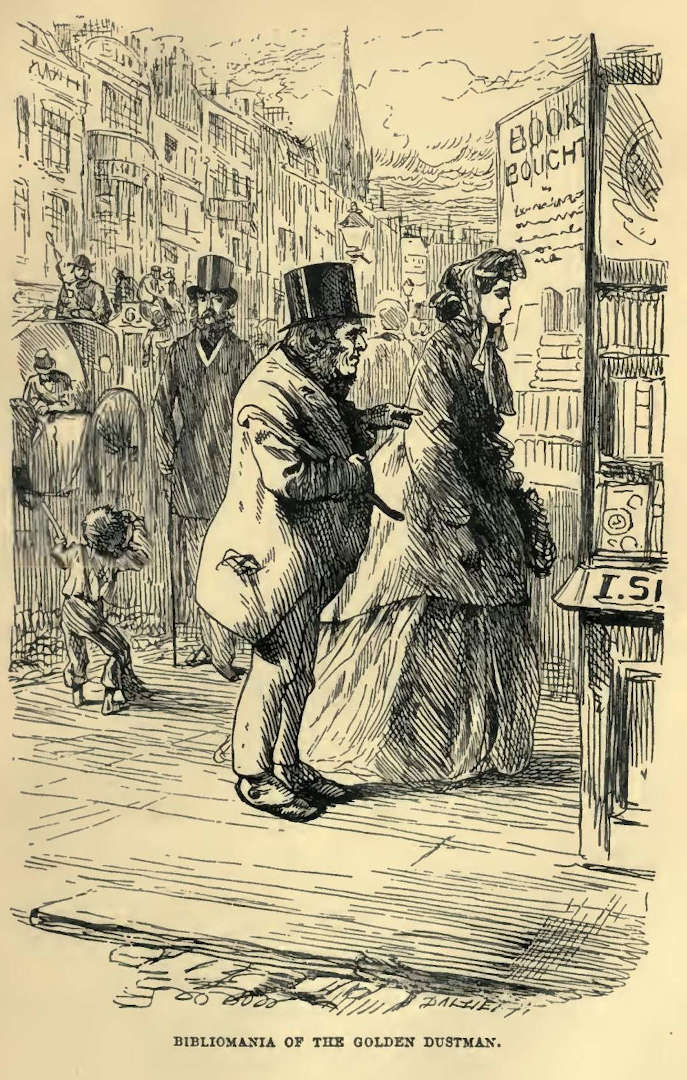
\includegraphics[scale=2.3]{03-05-01}

Chapter 7

THE FRIENDLY MOVE TAKES UP A STRONG POSITION


The friendly movers sat upright on the floor, panting and eyeing one
another, after Mr Boffin had slammed the gate and gone away. In the weak
eyes of Venus, and in every reddish dust-coloured hair in his shock of
hair, there was a marked distrust of Wegg and an alertness to fly at him
on perceiving the smallest occasion. In the hard-grained face of Wegg,
and in his stiff knotty figure (he looked like a German wooden toy),
there was expressed a politic conciliation, which had no spontaneity in
it. Both were flushed, flustered, and rumpled, by the late scuffle; and
Wegg, in coming to the ground, had received a humming knock on the back
of his devoted head, which caused him still to rub it with an air of
having been highly--but disagreeably--astonished. Each was silent for
some time, leaving it to the other to begin.

‘Brother,’ said Wegg, at length breaking the silence, ‘you were right,
and I was wrong. I forgot myself.’

Mr Venus knowingly cocked his shock of hair, as rather thinking Mr Wegg
had remembered himself, in respect of appearing without any disguise.

‘But comrade,’ pursued Wegg, ‘it was never your lot to know Miss
Elizabeth, Master George, Aunt Jane, nor Uncle Parker.’

Mr Venus admitted that he had never known those distinguished persons,
and added, in effect, that he had never so much as desired the honour of
their acquaintance.

‘Don’t say that, comrade!’ retorted Wegg: ‘No, don’t say that! Because,
without having known them, you never can fully know what it is to be
stimilated to frenzy by the sight of the Usurper.’

Offering these excusatory words as if they reflected great credit on
himself, Mr Wegg impelled himself with his hands towards a chair in
a corner of the room, and there, after a variety of awkward gambols,
attained a perpendicular position. Mr Venus also rose.

‘Comrade,’ said Wegg, ‘take a seat. Comrade, what a speaking countenance
is yours!’

Mr Venus involuntarily smoothed his countenance, and looked at his hand,
as if to see whether any of its speaking properties came off.

‘For clearly do I know, mark you,’ pursued Wegg, pointing his words
with his forefinger, ‘clearly do I know what question your expressive
features puts to me.’

‘What question?’ said Venus.

‘The question,’ returned Wegg, with a sort of joyful affability, ‘why
I didn’t mention sooner, that I had found something. Says your speaking
countenance to me: “Why didn’t you communicate that, when I first come
in this evening? Why did you keep it back till you thought Mr Boffin had
come to look for the article?” Your speaking countenance,’ said Wegg,
‘puts it plainer than language. Now, you can’t read in my face what
answer I give?’

‘No, I can’t,’ said Venus.

‘I knew it! And why not?’ returned Wegg, with the same joyful candour.
‘Because I lay no claims to a speaking countenance. Because I am well
aware of my deficiencies. All men are not gifted alike. But I can answer
in words. And in what words? These. I wanted to give you a delightful
sap--pur--IZE!’

Having thus elongated and emphasized the word Surprise, Mr Wegg shook
his friend and brother by both hands, and then clapped him on both
knees, like an affectionate patron who entreated him not to mention so
small a service as that which it had been his happy privilege to render.

‘Your speaking countenance,’ said Wegg, ‘being answered to its
satisfaction, only asks then, “What have you found?” Why, I hear it say
the words!’

‘Well?’ retorted Venus snappishly, after waiting in vain. ‘If you hear
it say the words, why don’t you answer it?’

‘Hear me out!’ said Wegg. ‘I’m a-going to. Hear me out! Man and brother,
partner in feelings equally with undertakings and actions, I have found
a cash-box.’

‘Where?’

‘--Hear me out!’ said Wegg. (He tried to reserve whatever he could, and,
whenever disclosure was forced upon him, broke into a radiant gush of
Hear me out.) ‘On a certain day, sir--’

‘When?’ said Venus bluntly.

‘N--no,’ returned Wegg, shaking his head at once observantly,
thoughtfully, and playfully. ‘No, sir! That’s not your expressive
countenance which asks that question. That’s your voice; merely your
voice. To proceed. On a certain day, sir, I happened to be walking in
the yard--taking my lonely round--for in the words of a friend of my own
family, the author of All’s Well arranged as a duett:

     “Deserted, as you will remember Mr Venus, by the waning
     moon,
     When stars, it will occur to you before I mention it, proclaim
     night’s cheerless noon,
     On tower, fort, or tented ground,
     The sentry walks his lonely round,
     The sentry walks:”

--under those circumstances, sir, I happened to be walking in the yard
early one afternoon, and happened to have an iron rod in my hand, with
which I have been sometimes accustomed to beguile the monotony of a
literary life, when I struck it against an object not necessary to
trouble you by naming--’

‘It is necessary. What object?’ demanded Venus, in a wrathful tone.

‘--Hear me out!’ said Wegg. ‘The Pump.--When I struck it against the
Pump, and found, not only that the top was loose and opened with a lid,
but that something in it rattled. That something, comrade, I discovered
to be a small flat oblong cash-box. Shall I say it was disappointingly
light?’

‘There were papers in it,’ said Venus.

‘There your expressive countenance speaks indeed!’ cried Wegg. ‘A
paper. The box was locked, tied up, and sealed, and on the outside was
a parchment label, with the writing, “MY WILL, JOHN HARMON, TEMPORARILY
DEPOSITED HERE.”’

‘We must know its contents,’ said Venus.

‘--Hear me out!’ cried Wegg. ‘I said so, and I broke the box open.’

‘Without coming to me!’ exclaimed Venus.

‘Exactly so, sir!’ returned Wegg, blandly and buoyantly. ‘I see I take
you with me! Hear, hear, hear! Resolved, as your discriminating good
sense perceives, that if you was to have a sap--pur--IZE, it should be
a complete one! Well, sir. And so, as you have honoured me by
anticipating, I examined the document. Regularly executed, regularly
witnessed, very short. Inasmuch as he has never made friends, and has
ever had a rebellious family, he, John Harmon, gives to Nicodemus Boffin
the Little Mound, which is quite enough for him, and gives the whole
rest and residue of his property to the Crown.’

‘The date of the will that has been proved, must be looked to,’ remarked
Venus. ‘It may be later than this one.’

‘--Hear me out!’ cried Wegg. ‘I said so. I paid a shilling (never mind
your sixpence of it) to look up that will. Brother, that will is dated
months before this will. And now, as a fellow-man, and as a partner in a
friendly move,’ added Wegg, benignantly taking him by both hands again,
and clapping him on both knees again, ‘say have I completed my labour of
love to your perfect satisfaction, and are you sap--pur--IZED?’

Mr Venus contemplated his fellow-man and partner with doubting eyes, and
then rejoined stiffly:

‘This is great news indeed, Mr Wegg. There’s no denying it. But I could
have wished you had told it me before you got your fright to-night, and
I could have wished you had ever asked me as your partner what we were
to do, before you thought you were dividing a responsibility.’

‘--Hear me out!’ cried Wegg. ‘I knew you was a-going to say so. But
alone I bore the anxiety, and alone I’ll bear the blame!’ This with an
air of great magnanimity.

‘No,’ said Venus. ‘Let’s see this will and this box.’

‘Do I understand, brother,’ returned Wegg with considerable reluctance,
‘that it is your wish to see this will and this--?’

Mr Venus smote the table with his hand.

‘--Hear me out!’ said Wegg. ‘Hear me out! I’ll go and fetch ‘em.’

After being some time absent, as if in his covetousness he could hardly
make up his mind to produce the treasure to his partner, he returned
with an old leathern hat-box, into which he had put the other box,
for the better preservation of commonplace appearances, and for the
disarming of suspicion. ‘But I don’t half like opening it here,’ said
Silas in a low voice, looking around: ‘he might come back, he may not be
gone; we don’t know what he may be up to, after what we’ve seen.’

‘There’s something in that,’ assented Venus. ‘Come to my place.’

Jealous of the custody of the box, and yet fearful of opening it under
the existing circumstances, Wegg hesitated. ‘Come, I tell you,’ repeated
Venus, chafing, ‘to my place.’ Not very well seeing his way to a
refusal, Mr Wegg then rejoined in a gush, ‘--Hear me out!--Certainly.’
So he locked up the Bower and they set forth: Mr Venus taking his arm,
and keeping it with remarkable tenacity.

They found the usual dim light burning in the window of Mr Venus’s
establishment, imperfectly disclosing to the public the usual pair
of preserved frogs, sword in hand, with their point of honour still
unsettled. Mr Venus had closed his shop door on coming out, and now
opened it with the key and shut it again as soon as they were within;
but not before he had put up and barred the shutters of the shop window.
‘No one can get in without being let in,’ said he then, ‘and we couldn’t
be more snug than here.’ So he raked together the yet warm cinders in
the rusty grate, and made a fire, and trimmed the candle on the little
counter. As the fire cast its flickering gleams here and there upon the
dark greasy walls; the Hindoo baby, the African baby, the articulated
English baby, the assortment of skulls, and the rest of the collection,
came starting to their various stations as if they had all been out,
like their master and were punctual in a general rendezvous to assist
at the secret. The French gentleman had grown considerably since Mr Wegg
last saw him, being now accommodated with a pair of legs and a head,
though his arms were yet in abeyance. To whomsoever the head had
originally belonged, Silas Wegg would have regarded it as a personal
favour if he had not cut quite so many teeth.

Silas took his seat in silence on the wooden box before the fire, and
Venus dropping into his low chair produced from among his skeleton
hands, his tea-tray and tea-cups, and put the kettle on. Silas inwardly
approved of these preparations, trusting they might end in Mr Venus’s
diluting his intellect.

‘Now, sir,’ said Venus, ‘all is safe and quiet. Let us see this
discovery.’

With still reluctant hands, and not without several glances towards the
skeleton hands, as if he mistrusted that a couple of them might spring
forth and clutch the document, Wegg opened the hat-box and revealed the
cash-box, opened the cash-box and revealed the will. He held a corner
of it tight, while Venus, taking hold of another corner, searchingly and
attentively read it.

‘Was I correct in my account of it, partner?’ said Mr Wegg at length.

‘Partner, you were,’ said Mr Venus.

Mr Wegg thereupon made an easy, graceful movement, as though he would
fold it up; but Mr Venus held on by his corner.

‘No, sir,’ said Mr Venus, winking his weak eyes and shaking his head.
‘No, partner. The question is now brought up, who is going to take care
of this. Do you know who is going to take care of this, partner?’

‘I am,’ said Wegg.

‘Oh dear no, partner,’ retorted Venus. ‘That’s a mistake. I am. Now look
here, Mr Wegg. I don’t want to have any words with you, and still less
do I want to have any anatomical pursuits with you.’

‘What do you mean?’ said Wegg, quickly.

‘I mean, partner,’ replied Venus, slowly, ‘that it’s hardly possible
for a man to feel in a more amiable state towards another man than I
do towards you at this present moment. But I am on my own ground, I am
surrounded by the trophies of my art, and my tools is very handy.’

‘What do you mean, Mr Venus?’ asked Wegg again.

‘I am surrounded, as I have observed,’ said Mr Venus, placidly, ‘by
the trophies of my art. They are numerous, my stock of human warious is
large, the shop is pretty well crammed, and I don’t just now want any
more trophies of my art. But I like my art, and I know how to exercise
my art.’

‘No man better,’ assented Mr Wegg, with a somewhat staggered air.

‘There’s the Miscellanies of several human specimens,’ said Venus,
‘(though you mightn’t think it) in the box on which you’re sitting.
There’s the Miscellanies of several human specimens, in the lovely
compo-one behind the door’; with a nod towards the French gentleman. ‘It
still wants a pair of arms. I DON’T say that I’m in any hurry for ‘em.’

‘You must be wandering in your mind, partner,’ Silas remonstrated.

‘You’ll excuse me if I wander,’ returned Venus; ‘I am sometimes rather
subject to it. I like my art, and I know how to exercise my art, and I
mean to have the keeping of this document.’

‘But what has that got to do with your art, partner?’ asked Wegg, in an
insinuating tone.

Mr Venus winked his chronically-fatigued eyes both at once, and
adjusting the kettle on the fire, remarked to himself, in a hollow
voice, ‘She’ll bile in a couple of minutes.’

Silas Wegg glanced at the kettle, glanced at the shelves, glanced at the
French gentleman behind the door, and shrank a little as he glanced at
Mr Venus winking his red eyes, and feeling in his waistcoat pocket--as
for a lancet, say--with his unoccupied hand. He and Venus were
necessarily seated close together, as each held a corner of the
document, which was but a common sheet of paper.

‘Partner,’ said Wegg, even more insinuatingly than before, ‘I propose
that we cut it in half, and each keep a half.’

Venus shook his shock of hair, as he replied, ‘It wouldn’t do to
mutilate it, partner. It might seem to be cancelled.’

‘Partner,’ said Wegg, after a silence, during which they had
contemplated one another, ‘don’t your speaking countenance say that
you’re a-going to suggest a middle course?’

Venus shook his shock of hair as he replied, ‘Partner, you have kept
this paper from me once. You shall never keep it from me again. I offer
you the box and the label to take care of, but I’ll take care of the
paper.’

Silas hesitated a little longer, and then suddenly releasing his corner,
and resuming his buoyant and benignant tone, exclaimed, ‘What’s life
without trustfulness! What’s a fellow-man without honour! You’re welcome
to it, partner, in a spirit of trust and confidence.’

Continuing to wink his red eyes both together--but in a self-communing
way, and without any show of triumph--Mr Venus folded the paper now left
in his hand, and locked it in a drawer behind him, and pocketed the key.
He then proposed ‘A cup of tea, partner?’ To which Mr Wegg returned,
‘Thank’ee, partner,’ and the tea was made and poured out.

‘Next,’ said Venus, blowing at his tea in his saucer, and looking over
it at his confidential friend, ‘comes the question, What’s the course to
be pursued?’

On this head, Silas Wegg had much to say. Silas had to say That, he
would beg to remind his comrade, brother, and partner, of the impressive
passages they had read that evening; of the evident parallel in Mr
Boffin’s mind between them and the late owner of the Bower, and the
present circumstances of the Bower; of the bottle; and of the box. That,
the fortunes of his brother and comrade, and of himself were evidently
made, inasmuch as they had but to put their price upon this document,
and get that price from the minion of fortune and the worm of the hour:
who now appeared to be less of a minion and more of a worm than had been
previously supposed. That, he considered it plain that such price was
stateable in a single expressive word, and that the word was, ‘Halves!’
That, the question then arose when ‘Halves!’ should be called. That,
here he had a plan of action to recommend, with a conditional clause.
That, the plan of action was that they should lie by with patience;
that, they should allow the Mounds to be gradually levelled and cleared
away, while retaining to themselves their present opportunity of
watching the process--which would be, he conceived, to put the trouble
and cost of daily digging and delving upon somebody else, while they
might nightly turn such complete disturbance of the dust to the account
of their own private investigations--and that, when the Mounds were
gone, and they had worked those chances for their own joint benefit
solely, they should then, and not before, explode on the minion and
worm. But here came the conditional clause, and to this he entreated the
special attention of his comrade, brother, and partner. It was not to
be borne that the minion and worm should carry off any of that property
which was now to be regarded as their own property. When he, Mr Wegg,
had seen the minion surreptitiously making off with that bottle, and its
precious contents unknown, he had looked upon him in the light of a mere
robber, and, as such, would have despoiled him of his ill-gotten gain,
but for the judicious interference of his comrade, brother, and partner.
Therefore, the conditional clause he proposed was, that, if the minion
should return in his late sneaking manner, and if, being closely
watched, he should be found to possess himself of anything, no matter
what, the sharp sword impending over his head should be instantly shown
him, he should be strictly examined as to what he knew or suspected,
should be severely handled by them his masters, and should be kept in
a state of abject moral bondage and slavery until the time when they
should see fit to permit him to purchase his freedom at the price of
half his possessions. If, said Mr Wegg by way of peroration, he had
erred in saying only ‘Halves!’ he trusted to his comrade, brother, and
partner not to hesitate to set him right, and to reprove his weakness.
It might be more according to the rights of things, to say
Two-thirds; it might be more according to the rights of things, to say
Three-fourths. On those points he was ever open to correction.

Mr Venus, having wafted his attention to this discourse over three
successive saucers of tea, signified his concurrence in the views
advanced. Inspirited hereby, Mr Wegg extended his right hand, and
declared it to be a hand which never yet. Without entering into more
minute particulars. Mr Venus, sticking to his tea, briefly professed his
belief as polite forms required of him, that it WAS a hand which never
yet. But contented himself with looking at it, and did not take it to
his bosom.

‘Brother,’ said Wegg, when this happy understanding was established, ‘I
should like to ask you something. You remember the night when I first
looked in here, and found you floating your powerful mind in tea?’

Still swilling tea, Mr Venus nodded assent.

‘And there you sit, sir,’ pursued Wegg with an air of thoughtful
admiration, ‘as if you had never left off! There you sit, sir, as if you
had an unlimited capacity of assimilating the flagrant article! There
you sit, sir, in the midst of your works, looking as if you’d been
called upon for Home, Sweet Home, and was obleeging the company!

     “A exile from home splendour dazzles in vain,
     O give you your lowly Preparations again,
     The birds stuffed so sweetly that can’t be expected to come at
     your call,
     Give you these with the peace of mind dearer than all.
     Home, Home, Home, sweet Home!”

--Be it ever,’ added Mr Wegg in prose as he glanced about the shop,
‘ever so ghastly, all things considered there’s no place like it.’

‘You said you’d like to ask something; but you haven’t asked it,’
remarked Venus, very unsympathetic in manner.

‘Your peace of mind,’ said Wegg, offering condolence, ‘your peace of
mind was in a poor way that night. HOW’S it going on? IS it looking up
at all?’

‘She does not wish,’ replied Mr Venus with a comical mixture of
indignant obstinacy and tender melancholy, ‘to regard herself, nor yet
to be regarded, in that particular light. There’s no more to be said.’

‘Ah, dear me, dear me!’ exclaimed Wegg with a sigh, but eyeing him while
pretending to keep him company in eyeing the fire, ‘such is Woman! And
I remember you said that night, sitting there as I sat here--said that
night when your peace of mind was first laid low, that you had taken an
interest in these very affairs. Such is coincidence!’

‘Her father,’ rejoined Venus, and then stopped to swallow more tea, ‘her
father was mixed up in them.’

‘You didn’t mention her name, sir, I think?’ observed Wegg, pensively.
‘No, you didn’t mention her name that night.’

‘Pleasant Riderhood.’

‘In--deed!’ cried Wegg. ‘Pleasant Riderhood. There’s something moving in
the name. Pleasant. Dear me! Seems to express what she might have
been, if she hadn’t made that unpleasant remark--and what she ain’t,
in consequence of having made it. Would it at all pour balm into your
wounds, Mr Venus, to inquire how you came acquainted with her?’

‘I was down at the water-side,’ said Venus, taking another gulp of
tea and mournfully winking at the fire--‘looking for parrots’--taking
another gulp and stopping.

Mr Wegg hinted, to jog his attention: ‘You could hardly have been out
parrot-shooting, in the British climate, sir?’

‘No, no, no,’ said Venus fretfully. ‘I was down at the water-side,
looking for parrots brought home by sailors, to buy for stuffing.’

‘Ay, ay, ay, sir!’

‘--And looking for a nice pair of rattlesnakes, to articulate for a
Museum--when I was doomed to fall in with her and deal with her. It was
just at the time of that discovery in the river. Her father had seen the
discovery being towed in the river. I made the popularity of the subject
a reason for going back to improve the acquaintance, and I have never
since been the man I was. My very bones is rendered flabby by brooding
over it. If they could be brought to me loose, to sort, I should hardly
have the face to claim ‘em as mine. To such an extent have I fallen off
under it.’

Mr Wegg, less interested than he had been, glanced at one particular
shelf in the dark.

‘Why I remember, Mr Venus,’ he said in a tone of friendly commiseration
‘(for I remember every word that falls from you, sir), I remember that
you said that night, you had got up there--and then your words was,
“Never mind.”’

‘--The parrot that I bought of her,’ said Venus, with a despondent rise
and fall of his eyes. ‘Yes; there it lies on its side, dried up; except
for its plumage, very like myself. I’ve never had the heart to prepare
it, and I never shall have now.’

With a disappointed face, Silas mentally consigned this parrot to
regions more than tropical, and, seeming for the time to have lost
his power of assuming an interest in the woes of Mr Venus, fell to
tightening his wooden leg as a preparation for departure: its gymnastic
performances of that evening having severely tried its constitution.

After Silas had left the shop, hat-box in hand, and had left Mr Venus
to lower himself to oblivion-point with the requisite weight of tea, it
greatly preyed on his ingenuous mind that he had taken this artist into
partnership at all. He bitterly felt that he had overreached himself in
the beginning, by grasping at Mr Venus’s mere straws of hints, now shown
to be worthless for his purpose. Casting about for ways and means of
dissolving the connexion without loss of money, reproaching himself for
having been betrayed into an avowal of his secret, and complimenting
himself beyond measure on his purely accidental good luck, he beguiled
the distance between Clerkenwell and the mansion of the Golden Dustman.

For, Silas Wegg felt it to be quite out of the question that he could
lay his head upon his pillow in peace, without first hovering over
Mr Boffin’s house in the superior character of its Evil Genius. Power
(unless it be the power of intellect or virtue) has ever the greatest
attraction for the lowest natures; and the mere defiance of the
unconscious house-front, with his power to strip the roof off the
inhabiting family like the roof of a house of cards, was a treat which
had a charm for Silas Wegg.

As he hovered on the opposite side of the street, exulting, the carriage
drove up.

‘There’ll shortly be an end of YOU,’ said Wegg, threatening it with the
hat-box. ‘YOUR varnish is fading.’

Mrs Boffin descended and went in.

‘Look out for a fall, my Lady Dustwoman,’ said Wegg.

Bella lightly descended, and ran in after her.

‘How brisk we are!’ said Wegg. ‘You won’t run so gaily to your old
shabby home, my girl. You’ll have to go there, though.’

A little while, and the Secretary came out.

‘I was passed over for you,’ said Wegg. ‘But you had better provide
yourself with another situation, young man.’

Mr Boffin’s shadow passed upon the blinds of three large windows as he
trotted down the room, and passed again as he went back.

‘Yoop!’ cried Wegg. ‘You’re there, are you? Where’s the bottle? You
would give your bottle for my box, Dustman!’

Having now composed his mind for slumber, he turned homeward. Such
was the greed of the fellow, that his mind had shot beyond halves,
two-thirds, three-fourths, and gone straight to spoliation of the whole.
‘Though that wouldn’t quite do,’ he considered, growing cooler as he got
away. ‘That’s what would happen to him if he didn’t buy us up. We should
get nothing by that.’

We so judge others by ourselves, that it had never come into his head
before, that he might not buy us up, and might prove honest, and prefer
to be poor. It caused him a slight tremor as it passed; but a very
slight one, for the idle thought was gone directly.

‘He’s grown too fond of money for that,’ said Wegg; ‘he’s grown too fond
of money.’ The burden fell into a strain or tune as he stumped along the
pavements. All the way home he stumped it out of the rattling streets,
PIANO with his own foot, and FORTE with his wooden leg, ‘He’s GROWN too
FOND of MONEY for THAT, he’s GROWN too FOND of MONEY.’

Even next day Silas soothed himself with this melodious strain, when he
was called out of bed at daybreak, to set open the yard-gate and admit
the train of carts and horses that came to carry off the little Mound.
And all day long, as he kept unwinking watch on the slow process which
promised to protract itself through many days and weeks, whenever
(to save himself from being choked with dust) he patrolled a little
cinderous beat he established for the purpose, without taking his eyes
from the diggers, he still stumped to the tune: He’s GROWN too FOND of
MONEY for THAT, he’s GROWN too FOND of MONEY.’



Chapter 8

THE END OF A LONG JOURNEY


The train of carts and horses came and went all day from dawn to
nightfall, making little or no daily impression on the heap of ashes,
though, as the days passed on, the heap was seen to be slowly melting.
My lords and gentlemen and honourable boards, when you in the course
of your dust-shovelling and cinder-raking have piled up a mountain of
pretentious failure, you must off with your honourable coats for the
removal of it, and fall to the work with the power of all the queen’s
horses and all the queen’s men, or it will come rushing down and bury us
alive.

Yes, verily, my lords and gentlemen and honourable boards, adapting your
Catechism to the occasion, and by God’s help so you must. For when we
have got things to the pass that with an enormous treasure at disposal
to relieve the poor, the best of the poor detest our mercies, hide their
heads from us, and shame us by starving to death in the midst of us, it
is a pass impossible of prosperity, impossible of continuance. It may
not be so written in the Gospel according to Podsnappery; you may not
‘find these words’ for the text of a sermon, in the Returns of the Board
of Trade; but they have been the truth since the foundations of the
universe were laid, and they will be the truth until the foundations of
the universe are shaken by the Builder. This boastful handiwork of
ours, which fails in its terrors for the professional pauper, the sturdy
breaker of windows and the rampant tearer of clothes, strikes with a
cruel and a wicked stab at the stricken sufferer, and is a horror to
the deserving and unfortunate. We must mend it, lords and gentlemen and
honourable boards, or in its own evil hour it will mar every one of us.

Old Betty Higden fared upon her pilgrimage as many ruggedly honest
creatures, women and men, fare on their toiling way along the roads
of life. Patiently to earn a spare bare living, and quietly to die,
untouched by workhouse hands--this was her highest sublunary hope.

Nothing had been heard of her at Mr Boffin’s house since she trudged
off. The weather had been hard and the roads had been bad, and her
spirit was up. A less stanch spirit might have been subdued by such
adverse influences; but the loan for her little outfit was in no part
repaid, and it had gone worse with her than she had foreseen, and she
was put upon proving her case and maintaining her independence.

Faithful soul! When she had spoken to the Secretary of that ‘deadness
that steals over me at times’, her fortitude had made too little of it.
Oftener and ever oftener, it came stealing over her; darker and ever
darker, like the shadow of advancing Death. That the shadow should
be deep as it came on, like the shadow of an actual presence, was in
accordance with the laws of the physical world, for all the Light that
shone on Betty Higden lay beyond Death.

The poor old creature had taken the upward course of the river Thames as
her general track; it was the track in which her last home lay, and of
which she had last had local love and knowledge. She had hovered for a
little while in the near neighbourhood of her abandoned dwelling, and
had sold, and knitted and sold, and gone on. In the pleasant towns of
Chertsey, Walton, Kingston, and Staines, her figure came to be quite
well known for some short weeks, and then again passed on.

She would take her stand in market-places, where there were such things,
on market days; at other times, in the busiest (that was seldom very
busy) portion of the little quiet High Street; at still other times she
would explore the outlying roads for great houses, and would ask leave
at the Lodge to pass in with her basket, and would not often get it. But
ladies in carriages would frequently make purchases from her trifling
stock, and were usually pleased with her bright eyes and her hopeful
speech. In these and her clean dress originated a fable that she was
well to do in the world: one might say, for her station, rich. As making
a comfortable provision for its subject which costs nobody anything,
this class of fable has long been popular.

In those pleasant little towns on Thames, you may hear the fall of
the water over the weirs, or even, in still weather, the rustle of the
rushes; and from the bridge you may see the young river, dimpled like a
young child, playfully gliding away among the trees, unpolluted by the
defilements that lie in wait for it on its course, and as yet out of
hearing of the deep summons of the sea. It were too much to pretend that
Betty Higden made out such thoughts; no; but she heard the tender river
whispering to many like herself, ‘Come to me, come to me! When the cruel
shame and terror you have so long fled from, most beset you, come to me!
I am the Relieving Officer appointed by eternal ordinance to do my work;
I am not held in estimation according as I shirk it. My breast is softer
than the pauper-nurse’s; death in my arms is peacefuller than among the
pauper-wards. Come to me!’

There was abundant place for gentler fancies too, in her untutored mind.
Those gentlefolks and their children inside those fine houses, could
they think, as they looked out at her, what it was to be really hungry,
really cold? Did they feel any of the wonder about her, that she felt
about them? Bless the dear laughing children! If they could have seen
sick Johnny in her arms, would they have cried for pity? If they could
have seen dead Johnny on that little bed, would they have understood it?
Bless the dear children for his sake, anyhow! So with the humbler houses
in the little street, the inner firelight shining on the panes as the
outer twilight darkened. When the families gathered in-doors there, for
the night, it was only a foolish fancy to feel as if it were a little
hard in them to close the shutter and blacken the flame. So with the
lighted shops, and speculations whether their masters and mistresses
taking tea in a perspective of back-parlour--not so far within but that
the flavour of tea and toast came out, mingled with the glow of light,
into the street--ate or drank or wore what they sold, with the greater
relish because they dealt in it. So with the churchyard on a branch of
the solitary way to the night’s sleeping-place. ‘Ah me! The dead and
I seem to have it pretty much to ourselves in the dark and in this
weather! But so much the better for all who are warmly housed at home.’
The poor soul envied no one in bitterness, and grudged no one anything.

But, the old abhorrence grew stronger on her as she grew weaker, and
it found more sustaining food than she did in her wanderings. Now, she
would light upon the shameful spectacle of some desolate creature--or
some wretched ragged groups of either sex, or of both sexes, with
children among them, huddled together like the smaller vermin for
a little warmth--lingering and lingering on a doorstep, while the
appointed evader of the public trust did his dirty office of trying to
weary them out and so get rid of them. Now, she would light upon some
poor decent person, like herself, going afoot on a pilgrimage of
many weary miles to see some worn-out relative or friend who had been
charitably clutched off to a great blank barren Union House, as far from
old home as the County Jail (the remoteness of which is always its worst
punishment for small rural offenders), and in its dietary, and in
its lodging, and in its tending of the sick, a much more penal
establishment. Sometimes she would hear a newspaper read out, and would
learn how the Registrar General cast up the units that had within the
last week died of want and of exposure to the weather: for which that
Recording Angel seemed to have a regular fixed place in his sum, as if
they were its halfpence. All such things she would hear discussed, as
we, my lords and gentlemen and honourable boards, in our unapproachable
magnificence never hear them, and from all such things she would fly
with the wings of raging Despair.

This is not to be received as a figure of speech. Old Betty Higden
however tired, however footsore, would start up and be driven away
by her awakened horror of falling into the hands of Charity. It is a
remarkable Christian improvement, to have made a pursuing Fury of the
Good Samaritan; but it was so in this case, and it is a type of many,
many, many.

Two incidents united to intensify the old unreasoning
abhorrence--granted in a previous place to be unreasoning, because the
people always are unreasoning, and invariably make a point of producing
all their smoke without fire.

One day she was sitting in a market-place on a bench outside an inn,
with her little wares for sale, when the deadness that she strove
against came over her so heavily that the scene departed from before
her eyes; when it returned, she found herself on the ground, her head
supported by some good-natured market-women, and a little crowd about
her.

‘Are you better now, mother?’ asked one of the women. ‘Do you think you
can do nicely now?’

‘Have I been ill then?’ asked old Betty.

‘You have had a faint like,’ was the answer, ‘or a fit. It ain’t that
you’ve been a-struggling, mother, but you’ve been stiff and numbed.’

‘Ah!’ said Betty, recovering her memory. ‘It’s the numbness. Yes. It
comes over me at times.’

Was it gone? the women asked her.

‘It’s gone now,’ said Betty. ‘I shall be stronger than I was afore.
Many thanks to ye, my dears, and when you come to be as old as I am, may
others do as much for you!’

They assisted her to rise, but she could not stand yet, and they
supported her when she sat down again upon the bench.

‘My head’s a bit light, and my feet are a bit heavy,’ said old Betty,
leaning her face drowsily on the breast of the woman who had spoken
before. ‘They’ll both come nat’ral in a minute. There’s nothing more the
matter.’

‘Ask her,’ said some farmers standing by, who had come out from their
market-dinner, ‘who belongs to her.’

‘Are there any folks belonging to you, mother?’ said the woman.

‘Yes sure,’ answered Betty. ‘I heerd the gentleman say it, but I
couldn’t answer quick enough. There’s plenty belonging to me. Don’t ye
fear for me, my dear.’

‘But are any of ‘em near here?’ said the men’s voices; the women’s
voices chiming in when it was said, and prolonging the strain.

‘Quite near enough,’ said Betty, rousing herself. ‘Don’t ye be afeard
for me, neighbours.’

‘But you are not fit to travel. Where are you going?’ was the next
compassionate chorus she heard.

‘I’m a going to London when I’ve sold out all,’ said Betty, rising with
difficulty. ‘I’ve right good friends in London. I want for nothing. I
shall come to no harm. Thankye. Don’t ye be afeard for me.’

A well-meaning bystander, yellow-legginged and purple-faced, said
hoarsely over his red comforter, as she rose to her feet, that she
‘oughtn’t to be let to go’.

‘For the Lord’s love don’t meddle with me!’ cried old Betty, all her
fears crowding on her. ‘I am quite well now, and I must go this minute.’

She caught up her basket as she spoke and was making an unsteady rush
away from them, when the same bystander checked her with his hand on
her sleeve, and urged her to come with him and see the parish-doctor.
Strengthening herself by the utmost exercise of her resolution, the poor
trembling creature shook him off, almost fiercely, and took to flight.
Nor did she feel safe until she had set a mile or two of by-road between
herself and the marketplace, and had crept into a copse, like a hunted
animal, to hide and recover breath. Not until then for the first time
did she venture to recall how she had looked over her shoulder before
turning out of the town, and had seen the sign of the White Lion hanging
across the road, and the fluttering market booths, and the old grey
church, and the little crowd gazing after her but not attempting to
follow her.

The second frightening incident was this. She had been again as bad, and
had been for some days better, and was travelling along by a part of
the road where it touched the river, and in wet seasons was so often
overflowed by it that there were tall white posts set up to mark the
way. A barge was being towed towards her, and she sat down on the bank
to rest and watch it. As the tow-rope was slackened by a turn of the
stream and dipped into the water, such a confusion stole into her
mind that she thought she saw the forms of her dead children and dead
grandchildren peopling the barge, and waving their hands to her in
solemn measure; then, as the rope tightened and came up, dropping
diamonds, it seemed to vibrate into two parallel ropes and strike her,
with a twang, though it was far off. When she looked again, there was no
barge, no river, no daylight, and a man whom she had never before seen
held a candle close to her face.

‘Now, Missis,’ said he; ‘where did you come from and where are you going
to?’

The poor soul confusedly asked the counter-question where she was?

‘I am the Lock,’ said the man.

‘The Lock?’

‘I am the Deputy Lock, on job, and this is the Lock-house. (Lock or
Deputy Lock, it’s all one, while the t’other man’s in the hospital.)
What’s your Parish?’

‘Parish!’ She was up from the truckle-bed directly, wildly feeling about
her for her basket, and gazing at him in affright.

‘You’ll be asked the question down town,’ said the man. ‘They won’t let
you be more than a Casual there. They’ll pass you on to your settlement,
Missis, with all speed. You’re not in a state to be let come upon
strange parishes ‘ceptin as a Casual.’

‘’Twas the deadness again!’ murmured Betty Higden, with her hand to her
head.

‘It was the deadness, there’s not a doubt about it,’ returned the man.
‘I should have thought the deadness was a mild word for it, if it had
been named to me when we brought you in. Have you got any friends,
Missis?’

‘The best of friends, Master.’

‘I should recommend your looking ‘em up if you consider ‘em game to do
anything for you,’ said the Deputy Lock. ‘Have you got any money?’

‘Just a morsel of money, sir.’

‘Do you want to keep it?’

‘Sure I do!’

‘Well, you know,’ said the Deputy Lock, shrugging his shoulders with his
hands in his pockets, and shaking his head in a sulkily ominous manner,
‘the parish authorities down town will have it out of you, if you go on,
you may take your Alfred David.’

‘Then I’ll not go on.’

‘They’ll make you pay, as fur as your money will go,’ pursued the
Deputy, ‘for your relief as a Casual and for your being passed to your
Parish.’

‘Thank ye kindly, Master, for your warning, thank ye for your shelter,
and good night.’

‘Stop a bit,’ said the Deputy, striking in between her and the door.
‘Why are you all of a shake, and what’s your hurry, Missis?’

‘Oh, Master, Master,’ returned Betty Higden, ‘I’ve fought against the
Parish and fled from it, all my life, and I want to die free of it!’

‘I don’t know,’ said the Deputy, with deliberation, ‘as I ought to let
you go. I’m a honest man as gets my living by the sweat of my brow, and
I may fall into trouble by letting you go. I’ve fell into trouble afore
now, by George, and I know what it is, and it’s made me careful. You
might be took with your deadness again, half a mile off--or half of half
a quarter, for the matter of that--and then it would be asked, Why did
that there honest Deputy Lock, let her go, instead of putting her safe
with the Parish? That’s what a man of his character ought to have done,
it would be argueyfied,’ said the Deputy Lock, cunningly harping on the
strong string of her terror; ‘he ought to have handed her over safe to
the Parish. That was to be expected of a man of his merits.’

As he stood in the doorway, the poor old careworn wayworn woman burst
into tears, and clasped her hands, as if in a very agony she prayed to
him.

‘As I’ve told you, Master, I’ve the best of friends. This letter will
show how true I spoke, and they will be thankful for me.’

The Deputy Lock opened the letter with a grave face, which underwent no
change as he eyed its contents. But it might have done, if he could have
read them.

‘What amount of small change, Missis,’ he said, with an abstracted air,
after a little meditation, ‘might you call a morsel of money?’

Hurriedly emptying her pocket, old Betty laid down on the table, a
shilling, and two sixpenny pieces, and a few pence.

‘If I was to let you go instead of handing you over safe to the Parish,’
said the Deputy, counting the money with his eyes, ‘might it be your own
free wish to leave that there behind you?’

‘Take it, Master, take it, and welcome and thankful!’

‘I’m a man,’ said the Deputy, giving her back the letter, and pocketing
the coins, one by one, ‘as earns his living by the sweat of his brow;’
here he drew his sleeve across his forehead, as if this particular
portion of his humble gains were the result of sheer hard labour and
virtuous industry; ‘and I won’t stand in your way. Go where you like.’

She was gone out of the Lock-house as soon as he gave her this
permission, and her tottering steps were on the road again. But, afraid
to go back and afraid to go forward; seeing what she fled from, in the
sky-glare of the lights of the little town before her, and leaving a
confused horror of it everywhere behind her, as if she had escaped it
in every stone of every market-place; she struck off by side ways, among
which she got bewildered and lost. That night she took refuge from the
Samaritan in his latest accredited form, under a farmer’s rick; and
if--worth thinking of, perhaps, my fellow-Christians--the Samaritan had
in the lonely night, ‘passed by on the other side’, she would have most
devoutly thanked High Heaven for her escape from him.

The morning found her afoot again, but fast declining as to the
clearness of her thoughts, though not as to the steadiness of her
purpose. Comprehending that her strength was quitting her, and that the
struggle of her life was almost ended, she could neither reason out the
means of getting back to her protectors, nor even form the idea. The
overmastering dread, and the proud stubborn resolution it engendered
in her to die undegraded, were the two distinct impressions left in her
failing mind. Supported only by a sense that she was bent on conquering
in her life-long fight, she went on.

The time was come, now, when the wants of this little life were passing
away from her. She could not have swallowed food, though a table had
been spread for her in the next field. The day was cold and wet, but
she scarcely knew it. She crept on, poor soul, like a criminal afraid of
being taken, and felt little beyond the terror of falling down while it
was yet daylight, and being found alive. She had no fear that she would
live through another night.

Sewn in the breast of her gown, the money to pay for her burial was
still intact. If she could wear through the day, and then lie down to
die under cover of the darkness, she would die independent. If she were
captured previously, the money would be taken from her as a pauper who
had no right to it, and she would be carried to the accursed workhouse.
Gaining her end, the letter would be found in her breast, along with
the money, and the gentlefolks would say when it was given back to them,
‘She prized it, did old Betty Higden; she was true to it; and while she
lived, she would never let it be disgraced by falling into the hands
of those that she held in horror.’ Most illogical, inconsequential, and
light-headed, this; but travellers in the valley of the shadow of death
are apt to be light-headed; and worn-out old people of low estate have
a trick of reasoning as indifferently as they live, and doubtless
would appreciate our Poor Law more philosophically on an income of ten
thousand a year.

So, keeping to byways, and shunning human approach, this troublesome
old woman hid herself, and fared on all through the dreary day. Yet so
unlike was she to vagrant hiders in general, that sometimes, as the day
advanced, there was a bright fire in her eyes, and a quicker beating at
her feeble heart, as though she said exultingly, ‘The Lord will see me
through it!’

By what visionary hands she was led along upon that journey of escape
from the Samaritan; by what voices, hushed in the grave, she seemed
to be addressed; how she fancied the dead child in her arms again, and
times innumerable adjusted her shawl to keep it warm; what infinite
variety of forms of tower and roof and steeple the trees took; how many
furious horsemen rode at her, crying, ‘There she goes! Stop! Stop,
Betty Higden!’ and melted away as they came close; be these things left
untold. Faring on and hiding, hiding and faring on, the poor harmless
creature, as though she were a Murderess and the whole country were up
after her, wore out the day, and gained the night.

‘Water-meadows, or such like,’ she had sometimes murmured, on the day’s
pilgrimage, when she had raised her head and taken any note of the real
objects about her. There now arose in the darkness, a great building,
full of lighted windows. Smoke was issuing from a high chimney in
the rear of it, and there was the sound of a water-wheel at the side.
Between her and the building, lay a piece of water, in which the lighted
windows were reflected, and on its nearest margin was a plantation of
trees. ‘I humbly thank the Power and the Glory,’ said Betty Higden,
holding up her withered hands, ‘that I have come to my journey’s end!’

She crept among the trees to the trunk of a tree whence she could see,
beyond some intervening trees and branches, the lighted windows, both in
their reality and their reflection in the water. She placed her orderly
little basket at her side, and sank upon the ground, supporting herself
against the tree. It brought to her mind the foot of the Cross, and
she committed herself to Him who died upon it. Her strength held out to
enable her to arrange the letter in her breast, so as that it could
be seen that she had a paper there. It had held out for this, and it
departed when this was done.

‘I am safe here,’ was her last benumbed thought. ‘When I am found dead
at the foot of the Cross, it will be by some of my own sort; some of
the working people who work among the lights yonder. I cannot see the
lighted windows now, but they are there. I am thankful for all!’


The darkness gone, and a face bending down.

‘It cannot be the boofer lady?’

‘I don’t understand what you say. Let me wet your lips again with this
brandy. I have been away to fetch it. Did you think that I was long
gone?’

It is as the face of a woman, shaded by a quantity of rich dark hair.
It is the earnest face of a woman who is young and handsome. But all is
over with me on earth, and this must be an Angel.

‘Have I been long dead?’

‘I don’t understand what you say. Let me wet your lips again. I hurried
all I could, and brought no one back with me, lest you should die of the
shock of strangers.’

‘Am I not dead?’

‘I cannot understand what you say. Your voice is so low and broken that
I cannot hear you. Do you hear me?’

‘Yes.’

‘Do you mean Yes?’

‘Yes.’

‘I was coming from my work just now, along the path outside (I was up
with the night-hands last night), and I heard a groan, and found you
lying here.’

‘What work, deary?’

‘Did you ask what work? At the paper-mill.’

‘Where is it?’

‘Your face is turned up to the sky, and you can’t see it. It is close
by. You can see my face, here, between you and the sky?’

‘Yes.’

‘Dare I lift you?’

‘Not yet.’

‘Not even lift your head to get it on my arm? I will do it by very
gentle degrees. You shall hardly feel it.’

‘Not yet. Paper. Letter.’

‘This paper in your breast?’

‘Bless ye!’

‘Let me wet your lips again. Am I to open it? To read it?’

‘Bless ye!’

She reads it with surprise, and looks down with a new expression and an
added interest on the motionless face she kneels beside.

‘I know these names. I have heard them often.’

‘Will you send it, my dear?’

‘I cannot understand you. Let me wet your lips again, and your forehead.
There. O poor thing, poor thing!’ These words through her fast-dropping
tears. ‘What was it that you asked me? Wait till I bring my ear quite
close.’

‘Will you send it, my dear?’

‘Will I send it to the writers? Is that your wish? Yes, certainly.’

‘You’ll not give it up to any one but them?’

‘No.’

‘As you must grow old in time, and come to your dying hour, my dear,
you’ll not give it up to any one but them?’

‘No. Most solemnly.’

‘Never to the Parish!’ with a convulsed struggle.

‘No. Most solemnly.’

‘Nor let the Parish touch me, not yet so much as look at me!’ with
another struggle.

‘No. Faithfully.’

A look of thankfulness and triumph lights the worn old face.

The eyes, which have been darkly fixed upon the sky, turn with meaning
in them towards the compassionate face from which the tears are
dropping, and a smile is on the aged lips as they ask:

‘What is your name, my dear?’

‘My name is Lizzie Hexam.’

‘I must be sore disfigured. Are you afraid to kiss me?’

The answer is, the ready pressure of her lips upon the cold but smiling
mouth.

‘Bless ye! NOW lift me, my love.’

Lizzie Hexam very softly raised the weather-stained grey head, and
lifted her as high as Heaven.



Chapter 9

SOMEBODY BECOMES THE SUBJECT OF A PREDICTION


‘“We give thee hearty thanks for that it hath pleased thee to deliver
this our sister out of the miseries of this sinful world.”’ So read the
Reverend Frank Milvey in a not untroubled voice, for his heart misgave
him that all was not quite right between us and our sister--or say our
sister in Law--Poor Law--and that we sometimes read these words in an
awful manner, over our Sister and our Brother too.

And Sloppy--on whom the brave deceased had never turned her back until
she ran away from him, knowing that otherwise he would not be separated
from her--Sloppy could not in his conscience as yet find the hearty
thanks required of it. Selfish in Sloppy, and yet excusable, it may be
humbly hoped, because our sister had been more than his mother.

The words were read above the ashes of Betty Higden, in a corner of a
churchyard near the river; in a churchyard so obscure that there was
nothing in it but grass-mounds, not so much as one single tombstone.
It might not be to do an unreasonably great deal for the diggers and
hewers, in a registering age, if we ticketed their graves at the common
charge; so that a new generation might know which was which: so that the
soldier, sailor, emigrant, coming home, should be able to identify the
resting-place of father, mother, playmate, or betrothed. For, we turn up
our eyes and say that we are all alike in death, and we might turn
them down and work the saying out in this world, so far. It would
be sentimental, perhaps? But how say ye, my lords and gentleman and
honourable boards, shall we not find good standing-room left for a
little sentiment, if we look into our crowds?

Near unto the Reverend Frank Milvey as he read, stood his little wife,
John Rokesmith the Secretary, and Bella Wilfer. These, over and above
Sloppy, were the mourners at the lowly grave. Not a penny had been
added to the money sewn in her dress: what her honest spirit had so long
projected, was fulfilled.

‘I’ve took it in my head,’ said Sloppy, laying it, inconsolable, against
the church door, when all was done: ‘I’ve took it in my wretched head
that I might have sometimes turned a little harder for her, and it cuts
me deep to think so now.’

The Reverend Frank Milvey, comforting Sloppy, expounded to him how the
best of us were more or less remiss in our turnings at our respective
Mangles--some of us very much so--and how we were all a halting,
failing, feeble, and inconstant crew.

‘SHE warn’t, sir,’ said Sloppy, taking this ghostly counsel rather ill,
in behalf of his late benefactress. ‘Let us speak for ourselves, sir.
She went through with whatever duty she had to do. She went through with
me, she went through with the Minders, she went through with herself,
she went through with everythink. O Mrs Higden, Mrs Higden, you was a
woman and a mother and a mangler in a million million!’

With those heartfelt words, Sloppy removed his dejected head from the
church door, and took it back to the grave in the corner, and laid it
down there, and wept alone. ‘Not a very poor grave,’ said the Reverend
Frank Milvey, brushing his hand across his eyes, ‘when it has that
homely figure on it. Richer, I think, than it could be made by most of
the sculpture in Westminster Abbey!’

They left him undisturbed, and passed out at the wicket-gate. The
water-wheel of the paper-mill was audible there, and seemed to have a
softening influence on the bright wintry scene. They had arrived but a
little while before, and Lizzie Hexam now told them the little she could
add to the letter in which she had enclosed Mr Rokesmith’s letter and
had asked for their instructions. This was merely how she had heard the
groan, and what had afterwards passed, and how she had obtained leave
for the remains to be placed in that sweet, fresh, empty store-room of
the mill from which they had just accompanied them to the churchyard,
and how the last requests had been religiously observed.

‘I could not have done it all, or nearly all, of myself,’ said Lizzie.
‘I should not have wanted the will; but I should not have had the power,
without our managing partner.’

‘Surely not the Jew who received us?’ said Mrs Milvey.

[‘My dear,’ observed her husband in parenthesis, ‘why not?’)

‘The gentleman certainly is a Jew,’ said Lizzie, ‘and the lady, his
wife, is a Jewess, and I was first brought to their notice by a Jew. But
I think there cannot be kinder people in the world.’

‘But suppose they try to convert you!’ suggested Mrs Milvey, bristling
in her good little way, as a clergyman’s wife.

‘To do what, ma’am?’ asked Lizzie, with a modest smile.

‘To make you change your religion,’ said Mrs Milvey.

Lizzie shook her head, still smiling. ‘They have never asked me what
my religion is. They asked me what my story was, and I told them. They
asked me to be industrious and faithful, and I promised to be so.
They most willingly and cheerfully do their duty to all of us who are
employed here, and we try to do ours to them. Indeed they do much more
than their duty to us, for they are wonderfully mindful of us in many
ways.’

‘It is easy to see you’re a favourite, my dear,’ said little Mrs Milvey,
not quite pleased.

‘It would be very ungrateful in me to say I am not,’ returned Lizzie,
‘for I have been already raised to a place of confidence here. But that
makes no difference in their following their own religion and leaving
all of us to ours. They never talk of theirs to us, and they never talk
of ours to us. If I was the last in the mill, it would be just the same.
They never asked me what religion that poor thing had followed.’

‘My dear,’ said Mrs Milvey, aside to the Reverend Frank, ‘I wish you
would talk to her.’

‘My dear,’ said the Reverend Frank aside to his good little wife, ‘I
think I will leave it to somebody else. The circumstances are hardly
favourable. There are plenty of talkers going about, my love, and she
will soon find one.’

While this discourse was interchanging, both Bella and the Secretary
observed Lizzie Hexam with great attention. Brought face to face for the
first time with the daughter of his supposed murderer, it was natural
that John Harmon should have his own secret reasons for a careful
scrutiny of her countenance and manner. Bella knew that Lizzie’s
father had been falsely accused of the crime which had had so great an
influence on her own life and fortunes; and her interest, though it had
no secret springs, like that of the Secretary, was equally natural. Both
had expected to see something very different from the real Lizzie Hexam,
and thus it fell out that she became the unconscious means of bringing
them together.

For, when they had walked on with her to the little house in the clean
village by the paper-mill, where Lizzie had a lodging with an elderly
couple employed in the establishment, and when Mrs Milvey and Bella
had been up to see her room and had come down, the mill bell rang.
This called Lizzie away for the time, and left the Secretary and Bella
standing rather awkwardly in the small street; Mrs Milvey being engaged
in pursuing the village children, and her investigations whether they
were in danger of becoming children of Israel; and the Reverend Frank
being engaged--to say the truth--in evading that branch of his spiritual
functions, and getting out of sight surreptitiously.

Bella at length said:

‘Hadn’t we better talk about the commission we have undertaken, Mr
Rokesmith?’

‘By all means,’ said the Secretary.

‘I suppose,’ faltered Bella, ‘that we ARE both commissioned, or we
shouldn’t both be here?’

‘I suppose so,’ was the Secretary’s answer.

‘When I proposed to come with Mr and Mrs Milvey,’ said Bella, ‘Mrs
Boffin urged me to do so, in order that I might give her my small
report--it’s not worth anything, Mr Rokesmith, except for it’s being
a woman’s--which indeed with you may be a fresh reason for it’s being
worth nothing--of Lizzie Hexam.’

‘Mr Boffin,’ said the Secretary, ‘directed me to come for the same
purpose.’

As they spoke they were leaving the little street and emerging on the
wooded landscape by the river.

‘You think well of her, Mr Rokesmith?’ pursued Bella, conscious of
making all the advances.

‘I think highly of her.’

‘I am so glad of that! Something quite refined in her beauty, is there
not?’

‘Her appearance is very striking.’

‘There is a shade of sadness upon her that is quite touching. At least
I--I am not setting up my own poor opinion, you know, Mr Rokesmith,’
said Bella, excusing and explaining herself in a pretty shy way; ‘I am
consulting you.’

‘I noticed that sadness. I hope it may not,’ said the Secretary in
a lower voice, ‘be the result of the false accusation which has been
retracted.’

When they had passed on a little further without speaking, Bella, after
stealing a glance or two at the Secretary, suddenly said:

‘Oh, Mr Rokesmith, don’t be hard with me, don’t be stern with me; be
magnanimous! I want to talk with you on equal terms.’

The Secretary as suddenly brightened, and returned: ‘Upon my honour I
had no thought but for you. I forced myself to be constrained, lest you
might misinterpret my being more natural. There. It’s gone.’

‘Thank you,’ said Bella, holding out her little hand. ‘Forgive me.’

‘No!’ cried the Secretary, eagerly. ‘Forgive ME!’ For there were tears
in her eyes, and they were prettier in his sight (though they smote him
on the heart rather reproachfully too) than any other glitter in the
world.

When they had walked a little further:

‘You were going to speak to me,’ said the Secretary, with the shadow so
long on him quite thrown off and cast away, ‘about Lizzie Hexam. So was
I going to speak to you, if I could have begun.’

‘Now that you CAN begin, sir,’ returned Bella, with a look as if she
italicized the word by putting one of her dimples under it, ‘what were
you going to say?’

‘You remember, of course, that in her short letter to Mrs Boffin--short,
but containing everything to the purpose--she stipulated that either
her name, or else her place of residence, must be kept strictly a secret
among us.’

Bella nodded Yes.

‘It is my duty to find out why she made that stipulation. I have it in
charge from Mr Boffin to discover, and I am very desirous for myself to
discover, whether that retracted accusation still leaves any stain upon
her. I mean whether it places her at any disadvantage towards any one,
even towards herself.’

‘Yes,’ said Bella, nodding thoughtfully; ‘I understand. That seems wise,
and considerate.’

‘You may not have noticed, Miss Wilfer, that she has the same kind of
interest in you, that you have in her. Just as you are attracted by her
beaut--by her appearance and manner, she is attracted by yours.’

‘I certainly have NOT noticed it,’ returned Bella, again italicizing
with the dimple, ‘and I should have given her credit for--’

The Secretary with a smile held up his hand, so plainly interposing ‘not
for better taste’, that Bella’s colour deepened over the little piece of
coquetry she was checked in.

‘And so,’ resumed the Secretary, ‘if you would speak with her alone
before we go away from here, I feel quite sure that a natural and easy
confidence would arise between you. Of course you would not be asked to
betray it; and of course you would not, if you were. But if you do not
object to put this question to her--to ascertain for us her own feeling
in this one matter--you can do so at a far greater advantage than I or
any else could. Mr Boffin is anxious on the subject. And I am,’ added
the Secretary after a moment, ‘for a special reason, very anxious.’

‘I shall be happy, Mr Rokesmith,’ returned Bella, ‘to be of the least
use; for I feel, after the serious scene of to-day, that I am useless
enough in this world.’

‘Don’t say that,’ urged the Secretary.

‘Oh, but I mean that,’ said Bella, raising her eyebrows.

‘No one is useless in this world,’ retorted the Secretary, ‘who lightens
the burden of it for any one else.’

‘But I assure you I DON’T, Mr Rokesmith,’ said Bella, half-crying.

‘Not for your father?’

‘Dear, loving, self-forgetting, easily-satisfied Pa! Oh, yes! He thinks
so.’

‘It is enough if he only thinks so,’ said the Secretary. ‘Excuse the
interruption: I don’t like to hear you depreciate yourself.’

‘But YOU once depreciated ME, sir,’ thought Bella, pouting, ‘and I hope
you may be satisfied with the consequences you brought upon your head!’
However, she said nothing to that purpose; she even said something to a
different purpose.

‘Mr Rokesmith, it seems so long since we spoke together naturally, that
I am embarrassed in approaching another subject. Mr Boffin. You know I
am very grateful to him; don’t you? You know I feel a true respect for
him, and am bound to him by the strong ties of his own generosity; now
don’t you?’

‘Unquestionably. And also that you are his favourite companion.’

‘That makes it,’ said Bella, ‘so very difficult to speak of him. But--.
Does he treat you well?’

‘You see how he treats me,’ the Secretary answered, with a patient and
yet proud air.

‘Yes, and I see it with pain,’ said Bella, very energetically.

The Secretary gave her such a radiant look, that if he had thanked her a
hundred times, he could not have said as much as the look said.

‘I see it with pain,’ repeated Bella, ‘and it often makes me miserable.
Miserable, because I cannot bear to be supposed to approve of it, or
have any indirect share in it. Miserable, because I cannot bear to be
forced to admit to myself that Fortune is spoiling Mr Boffin.’

‘Miss Wilfer,’ said the Secretary, with a beaming face, ‘if you could
know with what delight I make the discovery that Fortune isn’t spoiling
YOU, you would know that it more than compensates me for any slight at
any other hands.’

‘Oh, don’t speak of ME,’ said Bella, giving herself an impatient little
slap with her glove. ‘You don’t know me as well as--’

‘As you know yourself?’ suggested the Secretary, finding that she
stopped. ‘DO you know yourself?’

‘I know quite enough of myself,’ said Bella, with a charming air of
being inclined to give herself up as a bad job, ‘and I don’t improve
upon acquaintance. But Mr Boffin.’

‘That Mr Boffin’s manner to me, or consideration for me, is not what it
used to be,’ observed the Secretary, ‘must be admitted. It is too plain
to be denied.’

‘Are you disposed to deny it, Mr Rokesmith?’ asked Bella, with a look of
wonder.

‘Ought I not to be glad to do so, if I could: though it were only for my
own sake?’

‘Truly,’ returned Bella, ‘it must try you very much, and--you must
please promise me that you won’t take ill what I am going to add, Mr
Rokesmith?’

‘I promise it with all my heart.’

‘--And it must sometimes, I should think,’ said Bella, hesitating, ‘a
little lower you in your own estimation?’

Assenting with a movement of his head, though not at all looking as if
it did, the Secretary replied:

‘I have very strong reasons, Miss Wilfer, for bearing with the drawbacks
of my position in the house we both inhabit. Believe that they are not
all mercenary, although I have, through a series of strange fatalities,
faded out of my place in life. If what you see with such a gracious
and good sympathy is calculated to rouse my pride, there are other
considerations (and those you do not see) urging me to quiet endurance.
The latter are by far the stronger.’

‘I think I have noticed, Mr Rokesmith,’ said Bella, looking at him with
curiosity, as not quite making him out, ‘that you repress yourself, and
force yourself, to act a passive part.’

‘You are right. I repress myself and force myself to act a part. It is
not in tameness of spirit that I submit. I have a settled purpose.’

‘And a good one, I hope,’ said Bella.

‘And a good one, I hope,’ he answered, looking steadily at her.

‘Sometimes I have fancied, sir,’ said Bella, turning away her eyes,
‘that your great regard for Mrs Boffin is a very powerful motive with
you.’

‘You are right again; it is. I would do anything for her, bear anything
for her. There are no words to express how I esteem that good, good
woman.’

‘As I do too! May I ask you one thing more, Mr Rokesmith?’

‘Anything more.’

‘Of course you see that she really suffers, when Mr Boffin shows how he
is changing?’

‘I see it, every day, as you see it, and am grieved to give her pain.’

‘To give her pain?’ said Bella, repeating the phrase quickly, with her
eyebrows raised.

‘I am generally the unfortunate cause of it.’

‘Perhaps she says to you, as she often says to me, that he is the best
of men, in spite of all.’

‘I often overhear her, in her honest and beautiful devotion to him,
saying so to you,’ returned the Secretary, with the same steady look,
‘but I cannot assert that she ever says so to me.’

Bella met the steady look for a moment with a wistful, musing little
look of her own, and then, nodding her pretty head several times, like
a dimpled philosopher (of the very best school) who was moralizing on
Life, heaved a little sigh, and gave up things in general for a bad job,
as she had previously been inclined to give up herself.

But, for all that, they had a very pleasant walk. The trees were bare of
leaves, and the river was bare of water-lilies; but the sky was not bare
of its beautiful blue, and the water reflected it, and a delicious
wind ran with the stream, touching the surface crisply. Perhaps the old
mirror was never yet made by human hands, which, if all the images it
has in its time reflected could pass across its surface again, would
fail to reveal some scene of horror or distress. But the great serene
mirror of the river seemed as if it might have reproduced all it had
ever reflected between those placid banks, and brought nothing to the
light save what was peaceful, pastoral, and blooming.

So, they walked, speaking of the newly filled-up grave, and of Johnny,
and of many things. So, on their return, they met brisk Mrs Milvey
coming to seek them, with the agreeable intelligence that there was no
fear for the village children, there being a Christian school in the
village, and no worse Judaical interference with it than to plant its
garden. So, they got back to the village as Lizzie Hexam was coming from
the paper-mill, and Bella detached herself to speak with her in her own
home.

‘I am afraid it is a poor room for you,’ said Lizzie, with a smile of
welcome, as she offered the post of honour by the fireside.

‘Not so poor as you think, my dear,’ returned Bella, ‘if you knew all.’
Indeed, though attained by some wonderful winding narrow stairs, which
seemed to have been erected in a pure white chimney, and though very low
in the ceiling, and very rugged in the floor, and rather blinking as
to the proportions of its lattice window, it was a pleasanter room than
that despised chamber once at home, in which Bella had first bemoaned
the miseries of taking lodgers.

The day was closing as the two girls looked at one another by the
fireside. The dusky room was lighted by the fire. The grate might have
been the old brazier, and the glow might have been the old hollow down
by the flare.

‘It’s quite new to me,’ said Lizzie, ‘to be visited by a lady so nearly
of my own age, and so pretty, as you. It’s a pleasure to me to look at
you.’

‘I have nothing left to begin with,’ returned Bella, blushing, ‘because
I was going to say that it was a pleasure to me to look at you, Lizzie.
But we can begin without a beginning, can’t we?’

Lizzie took the pretty little hand that was held out in as pretty a
little frankness.

‘Now, dear,’ said Bella, drawing her chair a little nearer, and taking
Lizzie’s arm as if they were going out for a walk, ‘I am commissioned
with something to say, and I dare say I shall say it wrong, but I
won’t if I can help it. It is in reference to your letter to Mr and Mrs
Boffin, and this is what it is. Let me see. Oh yes! This is what it is.’

With this exordium, Bella set forth that request of Lizzie’s touching
secrecy, and delicately spoke of that false accusation and its
retraction, and asked might she beg to be informed whether it had any
bearing, near or remote, on such request. ‘I feel, my dear,’ said Bella,
quite amazing herself by the business-like manner in which she was
getting on, ‘that the subject must be a painful one to you, but I
am mixed up in it also; for--I don’t know whether you may know it or
suspect it--I am the willed-away girl who was to have been married to
the unfortunate gentleman, if he had been pleased to approve of me. So
I was dragged into the subject without my consent, and you were dragged
into it without your consent, and there is very little to choose between
us.’

‘I had no doubt,’ said Lizzie, ‘that you were the Miss Wilfer I have
often heard named. Can you tell me who my unknown friend is?’

‘Unknown friend, my dear?’ said Bella.

‘Who caused the charge against poor father to be contradicted, and sent
me the written paper.’

Bella had never heard of him. Had no notion who he was.

‘I should have been glad to thank him,’ returned Lizzie. ‘He has done a
great deal for me. I must hope that he will let me thank him some day.
You asked me has it anything to do--’

‘It or the accusation itself,’ Bella put in.

‘Yes. Has either anything to do with my wishing to live quite secret and
retired here? No.’

As Lizzie Hexam shook her head in giving this reply and as her glance
sought the fire, there was a quiet resolution in her folded hands, not
lost on Bella’s bright eyes.

‘Have you lived much alone?’ asked Bella.

‘Yes. It’s nothing new to me. I used to be always alone many hours
together, in the day and in the night, when poor father was alive.’

‘You have a brother, I have been told?’

‘I have a brother, but he is not friendly with me. He is a very good
boy though, and has raised himself by his industry. I don’t complain of
him.’

As she said it, with her eyes upon the fire-glow, there was an
instantaneous escape of distress into her face. Bella seized the moment
to touch her hand.

‘Lizzie, I wish you would tell me whether you have any friend of your
own sex and age.’

‘I have lived that lonely kind of life, that I have never had one,’ was
the answer.

‘Nor I neither,’ said Bella. ‘Not that my life has been lonely, for I
could have sometimes wished it lonelier, instead of having Ma going on
like the Tragic Muse with a face-ache in majestic corners, and Lavvy
being spiteful--though of course I am very fond of them both. I wish
you could make a friend of me, Lizzie. Do you think you could? I have
no more of what they call character, my dear, than a canary-bird, but I
know I am trustworthy.’

The wayward, playful, affectionate nature, giddy for want of the
weight of some sustaining purpose, and capricious because it was always
fluttering among little things, was yet a captivating one. To Lizzie it
was so new, so pretty, at once so womanly and so childish, that it won
her completely. And when Bella said again, ‘Do you think you could,
Lizzie?’ with her eyebrows raised, her head inquiringly on one side,
and an odd doubt about it in her own bosom, Lizzie showed beyond all
question that she thought she could.

‘Tell me, my dear,’ said Bella, ‘what is the matter, and why you live
like this.’

Lizzie presently began, by way of prelude, ‘You must have many lovers--’
when Bella checked her with a little scream of astonishment.

‘My dear, I haven’t one!’

‘Not one?’

‘Well! Perhaps one,’ said Bella. ‘I am sure I don’t know. I HAD one, but
what he may think about it at the present time I can’t say. Perhaps I
have half a one (of course I don’t count that Idiot, George Sampson).
However, never mind me. I want to hear about you.’

‘There is a certain man,’ said Lizzie, ‘a passionate and angry man, who
says he loves me, and who I must believe does love me. He is the friend
of my brother. I shrank from him within myself when my brother first
brought him to me; but the last time I saw him he terrified me more than
I can say.’ There she stopped.

‘Did you come here to escape from him, Lizzie?’

‘I came here immediately after he so alarmed me.’

‘Are you afraid of him here?’

‘I am not timid generally, but I am always afraid of him. I am afraid
to see a newspaper, or to hear a word spoken of what is done in London,
lest he should have done some violence.’

‘Then you are not afraid of him for yourself, dear?’ said Bella, after
pondering on the words.

‘I should be even that, if I met him about here. I look round for him
always, as I pass to and fro at night.’

‘Are you afraid of anything he may do to himself in London, my dear?’

‘No. He might be fierce enough even to do some violence to himself, but
I don’t think of that.’

‘Then it would almost seem, dear,’ said Bella quaintly, ‘as if there
must be somebody else?’

Lizzie put her hands before her face for a moment before replying: ‘The
words are always in my ears, and the blow he struck upon a stone wall as
he said them is always before my eyes. I have tried hard to think it
not worth remembering, but I cannot make so little of it. His hand was
trickling down with blood as he said to me, “Then I hope that I may
never kill him!’

Rather startled, Bella made and clasped a girdle of her arms round
Lizzie’s waist, and then asked quietly, in a soft voice, as they both
looked at the fire:

‘Kill him! Is this man so jealous, then?’

‘Of a gentleman,’ said Lizzie. ‘--I hardly know how to tell you--of a
gentleman far above me and my way of life, who broke father’s death to
me, and has shown an interest in me since.’

‘Does he love you?’

Lizzie shook her head.

‘Does he admire you?’

Lizzie ceased to shake her head, and pressed her hand upon her living
girdle.

‘Is it through his influence that you came here?’

‘O no! And of all the world I wouldn’t have him know that I am here, or
get the least clue where to find me.’

‘Lizzie, dear! Why?’ asked Bella, in amazement at this burst. But then
quickly added, reading Lizzie’s face: ‘No. Don’t say why. That was a
foolish question of mine. I see, I see.’

There was silence between them. Lizzie, with a drooping head, glanced
down at the glow in the fire where her first fancies had been nursed,
and her first escape made from the grim life out of which she had
plucked her brother, foreseeing her reward.

‘You know all now,’ she said, raising her eyes to Bella’s. ‘There is
nothing left out. This is my reason for living secret here, with the aid
of a good old man who is my true friend. For a short part of my life
at home with father, I knew of things--don’t ask me what--that I set my
face against, and tried to better. I don’t think I could have done more,
then, without letting my hold on father go; but they sometimes lie heavy
on my mind. By doing all for the best, I hope I may wear them out.’

‘And wear out too,’ said Bella soothingly, ‘this weakness, Lizzie, in
favour of one who is not worthy of it.’

‘No. I don’t want to wear that out,’ was the flushed reply, ‘nor do I
want to believe, nor do I believe, that he is not worthy of it. What
should I gain by that, and how much should I lose!’

Bella’s expressive little eyebrows remonstrated with the fire for some
short time before she rejoined:

‘Don’t think that I press you, Lizzie; but wouldn’t you gain in peace,
and hope, and even in freedom? Wouldn’t it be better not to live a
secret life in hiding, and not to be shut out from your natural and
wholesome prospects? Forgive my asking you, would that be no gain?’

‘Does a woman’s heart that--that has that weakness in it which you have
spoken of,’ returned Lizzie, ‘seek to gain anything?’

The question was so directly at variance with Bella’s views in life, as
set forth to her father, that she said internally, ‘There, you little
mercenary wretch! Do you hear that? Ain’t you ashamed of your self?’
and unclasped the girdle of her arms, expressly to give herself a
penitential poke in the side.

‘But you said, Lizzie,’ observed Bella, returning to her subject when
she had administered this chastisement, ‘that you would lose, besides.
Would you mind telling me what you would lose, Lizzie?’

‘I should lose some of the best recollections, best encouragements,
and best objects, that I carry through my daily life. I should lose my
belief that if I had been his equal, and he had loved me, I should have
tried with all my might to make him better and happier, as he would have
made me. I should lose almost all the value that I put upon the little
learning I have, which is all owing to him, and which I conquered the
difficulties of, that he might not think it thrown away upon me. I
should lose a kind of picture of him--or of what he might have been,
if I had been a lady, and he had loved me--which is always with me, and
which I somehow feel that I could not do a mean or a wrong thing before.
I should leave off prizing the remembrance that he has done me nothing
but good since I have known him, and that he has made a change within
me, like--like the change in the grain of these hands, which were
coarse, and cracked, and hard, and brown when I rowed on the river with
father, and are softened and made supple by this new work as you see
them now.’

They trembled, but with no weakness, as she showed them.

‘Understand me, my dear;’ thus she went on. ‘I have never dreamed of
the possibility of his being anything to me on this earth but the
kind picture that I know I could not make you understand, if the
understanding was not in your own breast already. I have no more dreamed
of the possibility of MY being his wife, than he ever has--and words
could not be stronger than that. And yet I love him. I love him so much,
and so dearly, that when I sometimes think my life may be but a weary
one, I am proud of it and glad of it. I am proud and glad to suffer
something for him, even though it is of no service to him, and he will
never know of it or care for it.’

Bella sat enchained by the deep, unselfish passion of this girl or woman
of her own age, courageously revealing itself in the confidence of her
sympathetic perception of its truth. And yet she had never experienced
anything like it, or thought of the existence of anything like it.

‘It was late upon a wretched night,’ said Lizzie, ‘when his eyes first
looked at me in my old river-side home, very different from this. His
eyes may never look at me again. I would rather that they never did; I
hope that they never may. But I would not have the light of them taken
out of my life, for anything my life can give me. I have told you
everything now, my dear. If it comes a little strange to me to have
parted with it, I am not sorry. I had no thought of ever parting with a
single word of it, a moment before you came in; but you came in, and my
mind changed.’

Bella kissed her on the cheek, and thanked her warmly for her
confidence. ‘I only wish,’ said Bella, ‘I was more deserving of it.’

‘More deserving of it?’ repeated Lizzie, with an incredulous smile.

‘I don’t mean in respect of keeping it,’ said Bella, ‘because any
one should tear me to bits before getting at a syllable of it--though
there’s no merit in that, for I am naturally as obstinate as a Pig. What
I mean is, Lizzie, that I am a mere impertinent piece of conceit, and
you shame me.’

Lizzie put up the pretty brown hair that came tumbling down, owing to
the energy with which Bella shook her head; and she remonstrated while
thus engaged, ‘My dear!’

‘Oh, it’s all very well to call me your dear,’ said Bella, with a
pettish whimper, ‘and I am glad to be called so, though I have slight
enough claim to be. But I AM such a nasty little thing!’

‘My dear!’ urged Lizzie again.

‘Such a shallow, cold, worldly, Limited little brute!’ said Bella,
bringing out her last adjective with culminating force.

‘Do you think,’ inquired Lizzie with her quiet smile, the hair being now
secured, ‘that I don’t know better?’

‘DO you know better though?’ said Bella. ‘Do you really believe you know
better? Oh, I should be so glad if you did know better, but I am so very
much afraid that I must know best!’

Lizzie asked her, laughing outright, whether she ever saw her own face
or heard her own voice?

‘I suppose so,’ returned Bella; ‘I look in the glass often enough, and I
chatter like a Magpie.’

‘I have seen your face, and heard your voice, at any rate,’ said Lizzie,
‘and they have tempted me to say to you--with a certainty of not going
wrong--what I thought I should never say to any one. Does that look
ill?’

‘No, I hope it doesn’t,’ pouted Bella, stopping herself in something
between a humoured laugh and a humoured sob.

‘I used once to see pictures in the fire,’ said Lizzie playfully, ‘to
please my brother. Shall I tell you what I see down there where the fire
is glowing?’

They had risen, and were standing on the hearth, the time being come for
separating; each had drawn an arm around the other to take leave.

‘Shall I tell you,’ asked Lizzie, ‘what I see down there?’

‘Limited little b?’ suggested Bella with her eyebrows raised.

‘A heart well worth winning, and well won. A heart that, once won, goes
through fire and water for the winner, and never changes, and is never
daunted.’

‘Girl’s heart?’ asked Bella, with accompanying eyebrows.

Lizzie nodded. ‘And the figure to which it belongs--’

‘Is yours,’ suggested Bella.

‘No. Most clearly and distinctly yours.’

So the interview terminated with pleasant words on both sides, and with
many reminders on the part of Bella that they were friends, and pledges
that she would soon come down into that part of the country again. There
with Lizzie returned to her occupation, and Bella ran over to the little
inn to rejoin her company.

‘You look rather serious, Miss Wilfer,’ was the Secretary’s first
remark.

‘I feel rather serious,’ returned Miss Wilfer.

She had nothing else to tell him but that Lizzie Hexam’s secret had
no reference whatever to the cruel charge, or its withdrawal. Oh yes
though! said Bella; she might as well mention one other thing; Lizzie
was very desirous to thank her unknown friend who had sent her the
written retractation. Was she, indeed? observed the Secretary. Ah! Bella
asked him, had he any notion who that unknown friend might be? He had no
notion whatever.

They were on the borders of Oxfordshire, so far had poor old Betty
Higden strayed. They were to return by the train presently, and, the
station being near at hand, the Reverend Frank and Mrs Frank, and Sloppy
and Bella and the Secretary, set out to walk to it. Few rustic paths are
wide enough for five, and Bella and the Secretary dropped behind.

‘Can you believe, Mr Rokesmith,’ said Bella, ‘that I feel as if whole
years had passed since I went into Lizzie Hexam’s cottage?’

‘We have crowded a good deal into the day,’ he returned, ‘and you were
much affected in the churchyard. You are over-tired.’

‘No, I am not at all tired. I have not quite expressed what I mean. I
don’t mean that I feel as if a great space of time had gone by, but that
I feel as if much had happened--to myself, you know.’

‘For good, I hope?’

‘I hope so,’ said Bella.

‘You are cold; I felt you tremble. Pray let me put this wrapper of mine
about you. May I fold it over this shoulder without injuring your dress?
Now, it will be too heavy and too long. Let me carry this end over my
arm, as you have no arm to give me.’

Yes she had though. How she got it out, in her muffled state, Heaven
knows; but she got it out somehow--there it was--and slipped it through
the Secretary’s.

‘I have had a long and interesting talk with Lizzie, Mr Rokesmith, and
she gave me her full confidence.’

‘She could not withhold it,’ said the Secretary.

‘I wonder how you come,’ said Bella, stopping short as she glanced at
him, ‘to say to me just what she said about it!’

‘I infer that it must be because I feel just as she felt about it.’

‘And how was that, do you mean to say, sir?’ asked Bella, moving again.

‘That if you were inclined to win her confidence--anybody’s
confidence--you were sure to do it.’

The railway, at this point, knowingly shutting a green eye and opening
a red one, they had to run for it. As Bella could not run easily so
wrapped up, the Secretary had to help her. When she took her opposite
place in the carriage corner, the brightness in her face was so charming
to behold, that on her exclaiming, ‘What beautiful stars and what a
glorious night!’ the Secretary said ‘Yes,’ but seemed to prefer to see
the night and the stars in the light of her lovely little countenance,
to looking out of window.

O boofer lady, fascinating boofer lady! If I were but legally executor
of Johnny’s will! If I had but the right to pay your legacy and to take
your receipt!--Something to this purpose surely mingled with the blast
of the train as it cleared the stations, all knowingly shutting up their
green eyes and opening their red ones when they prepared to let the
boofer lady pass.



Chapter 10

SCOUTS OUT


‘And so, Miss Wren,’ said Mr Eugene Wrayburn, ‘I cannot persuade you to
dress me a doll?’

‘No,’ replied Miss Wren snappishly; ‘if you want one, go and buy one at
the shop.’

‘And my charming young goddaughter,’ said Mr Wrayburn plaintively, ‘down
in Hertfordshire--’

[‘Humbugshire you mean, I think,’ interposed Miss Wren.)

‘--is to be put upon the cold footing of the general public, and is
to derive no advantage from my private acquaintance with the Court
Dressmaker?’

‘If it’s any advantage to your charming godchild--and oh, a precious
godfather she has got!’--replied Miss Wren, pricking at him in the air
with her needle, ‘to be informed that the Court Dressmaker knows
your tricks and your manners, you may tell her so by post, with my
compliments.’

Miss Wren was busy at her work by candle-light, and Mr Wrayburn, half
amused and half vexed, and all idle and shiftless, stood by her bench
looking on. Miss Wren’s troublesome child was in the corner in deep
disgrace, and exhibiting great wretchedness in the shivering stage of
prostration from drink.

‘Ugh, you disgraceful boy!’ exclaimed Miss Wren, attracted by the sound
of his chattering teeth, ‘I wish they’d all drop down your throat and
play at dice in your stomach! Boh, wicked child! Bee-baa, black sheep!’

On her accompanying each of these reproaches with a threatening stamp of
the foot, the wretched creature protested with a whine.

‘Pay five shillings for you indeed!’ Miss Wren proceeded; ‘how many
hours do you suppose it costs me to earn five shillings, you infamous
boy?--Don’t cry like that, or I’ll throw a doll at you. Pay five
shillings fine for you indeed. Fine in more ways than one, I think! I’d
give the dustman five shillings, to carry you off in the dust cart.’

‘No, no,’ pleaded the absurd creature. ‘Please!’

‘He’s enough to break his mother’s heart, is this boy,’ said Miss Wren,
half appealing to Eugene. ‘I wish I had never brought him up. He’d be
sharper than a serpent’s tooth, if he wasn’t as dull as ditch water.
Look at him. There’s a pretty object for a parent’s eyes!’

Assuredly, in his worse than swinish state (for swine at least fatten on
their guzzling, and make themselves good to eat), he was a pretty object
for any eyes.

‘A muddling and a swipey old child,’ said Miss Wren, rating him with
great severity, ‘fit for nothing but to be preserved in the liquor
that destroys him, and put in a great glass bottle as a sight for other
swipey children of his own pattern,--if he has no consideration for his
liver, has he none for his mother?’

‘Yes. Deration, oh don’t!’ cried the subject of these angry remarks.

‘Oh don’t and oh don’t,’ pursued Miss Wren. ‘It’s oh do and oh do. And
why do you?’

‘Won’t do so any more. Won’t indeed. Pray!’

‘There!’ said Miss Wren, covering her eyes with her hand. ‘I can’t
bear to look at you. Go up stairs and get me my bonnet and shawl. Make
yourself useful in some way, bad boy, and let me have your room instead
of your company, for one half minute.’

Obeying her, he shambled out, and Eugene Wrayburn saw the tears exude
from between the little creature’s fingers as she kept her hand before
her eyes. He was sorry, but his sympathy did not move his carelessness
to do anything but feel sorry.

‘I’m going to the Italian Opera to try on,’ said Miss Wren, taking away
her hand after a little while, and laughing satirically to hide that she
had been crying; ‘I must see your back before I go, Mr Wrayburn. Let me
first tell you, once for all, that it’s of no use your paying visits
to me. You wouldn’t get what you want, of me, no, not if you brought
pincers with you to tear it out.’

‘Are you so obstinate on the subject of a doll’s dress for my godchild?’

‘Ah!’ returned Miss Wren with a hitch of her chin, ‘I am so
obstinate. And of course it’s on the subject of a doll’s dress--or
ADdress--whichever you like. Get along and give it up!’

Her degraded charge had come back, and was standing behind her with the
bonnet and shawl.

‘Give ‘em to me and get back into your corner, you naughty old thing!’
said Miss Wren, as she turned and espied him. ‘No, no, I won’t have your
help. Go into your corner, this minute!’

The miserable man, feebly rubbing the back of his faltering hands
downward from the wrists, shuffled on to his post of disgrace; but not
without a curious glance at Eugene in passing him, accompanied with what
seemed as if it might have been an action of his elbow, if any action of
any limb or joint he had, would have answered truly to his will. Taking
no more particular notice of him than instinctively falling away from
the disagreeable contact, Eugene, with a lazy compliment or so to Miss
Wren, begged leave to light his cigar, and departed.

‘Now you prodigal old son,’ said Jenny, shaking her head and her
emphatic little forefinger at her burden, ‘you sit there till I come
back. You dare to move out of your corner for a single instant while I’m
gone, and I’ll know the reason why.’

With this admonition, she blew her work candles out, leaving him to the
light of the fire, and, taking her big door-key in her pocket and her
crutch-stick in her hand, marched off.

Eugene lounged slowly towards the Temple, smoking his cigar, but saw
no more of the dolls’ dressmaker, through the accident of their taking
opposite sides of the street. He lounged along moodily, and stopped at
Charing Cross to look about him, with as little interest in the crowd
as any man might take, and was lounging on again, when a most unexpected
object caught his eyes. No less an object than Jenny Wren’s bad boy
trying to make up his mind to cross the road.

A more ridiculous and feeble spectacle than this tottering wretch making
unsteady sallies into the roadway, and as often staggering back again,
oppressed by terrors of vehicles that were a long way off or were
nowhere, the streets could not have shown. Over and over again, when the
course was perfectly clear, he set out, got half way, described a loop,
turned, and went back again; when he might have crossed and re-crossed
half a dozen times. Then, he would stand shivering on the edge of the
pavement, looking up the street and looking down, while scores of people
jostled him, and crossed, and went on. Stimulated in course of time
by the sight of so many successes, he would make another sally, make
another loop, would all but have his foot on the opposite pavement,
would see or imagine something coming, and would stagger back again.
There, he would stand making spasmodic preparations as if for a great
leap, and at last would decide on a start at precisely the wrong moment,
and would be roared at by drivers, and would shrink back once more, and
stand in the old spot shivering, with the whole of the proceedings to go
through again.

‘It strikes me,’ remarked Eugene coolly, after watching him for some
minutes, ‘that my friend is likely to be rather behind time if he has
any appointment on hand.’ With which remark he strolled on, and took no
further thought of him.

Lightwood was at home when he got to the Chambers, and had dined alone
there. Eugene drew a chair to the fire by which he was having his wine
and reading the evening paper, and brought a glass, and filled it for
good fellowship’s sake.

‘My dear Mortimer, you are the express picture of contented industry,
reposing (on credit) after the virtuous labours of the day.’

‘My dear Eugene, you are the express picture of discontented idleness
not reposing at all. Where have you been?’

‘I have been,’ replied Wrayburn, ‘--about town. I have turned up at the
present juncture, with the intention of consulting my highly intelligent
and respected solicitor on the position of my affairs.’

‘Your highly intelligent and respect solicitor is of opinion that your
affairs are in a bad way, Eugene.’

‘Though whether,’ said Eugene thoughtfully, ‘that can be intelligently
said, now, of the affairs of a client who has nothing to lose and who
cannot possibly be made to pay, may be open to question.’

‘You have fallen into the hands of the Jews, Eugene.’

‘My dear boy,’ returned the debtor, very composedly taking up his glass,
‘having previously fallen into the hands of some of the Christians, I
can bear it with philosophy.’

‘I have had an interview to-day, Eugene, with a Jew, who seems
determined to press us hard. Quite a Shylock, and quite a Patriarch. A
picturesque grey-headed and grey-bearded old Jew, in a shovel-hat and
gaberdine.’

‘Not,’ said Eugene, pausing in setting down his glass, ‘surely not my
worthy friend Mr Aaron?’

‘He calls himself Mr Riah.’

‘By-the-by,’ said Eugene, ‘it comes into my mind that--no doubt with an
instinctive desire to receive him into the bosom of our Church--I gave
him the name of Aaron!’

‘Eugene, Eugene,’ returned Lightwood, ‘you are more ridiculous than
usual. Say what you mean.’

‘Merely, my dear fellow, that I have the honour and pleasure of a
speaking acquaintance with such a Patriarch as you describe, and that I
address him as Mr Aaron, because it appears to me Hebraic, expressive,
appropriate, and complimentary. Notwithstanding which strong reasons for
its being his name, it may not be his name.’

‘I believe you are the absurdest man on the face of the earth,’ said
Lightwood, laughing.

‘Not at all, I assure you. Did he mention that he knew me?’

‘He did not. He only said of you that he expected to be paid by you.’

‘Which looks,’ remarked Eugene with much gravity, ‘like NOT knowing me.
I hope it may not be my worthy friend Mr Aaron, for, to tell you the
truth, Mortimer, I doubt he may have a prepossession against me. I
strongly suspect him of having had a hand in spiriting away Lizzie.’

‘Everything,’ returned Lightwood impatiently, ‘seems, by a fatality,
to bring us round to Lizzie. “About town” meant about Lizzie, just now,
Eugene.’

‘My solicitor, do you know,’ observed Eugene, turning round to the
furniture, ‘is a man of infinite discernment!’

‘Did it not, Eugene?’

‘Yes it did, Mortimer.’

‘And yet, Eugene, you know you do not really care for her.’

Eugene Wrayburn rose, and put his hands in his pockets, and stood with a
foot on the fender, indolently rocking his body and looking at the fire.
After a prolonged pause, he replied: ‘I don’t know that. I must ask you
not to say that, as if we took it for granted.’

‘But if you do care for her, so much the more should you leave her to
herself.’

Having again paused as before, Eugene said: ‘I don’t know that, either.
But tell me. Did you ever see me take so much trouble about anything, as
about this disappearance of hers? I ask, for information.’

‘My dear Eugene, I wish I ever had!’

‘Then you have not? Just so. You confirm my own impression. Does that
look as if I cared for her? I ask, for information.’

‘I asked YOU for information, Eugene,’ said Mortimer reproachfully.

‘Dear boy, I know it, but I can’t give it. I thirst for information.
What do I mean? If my taking so much trouble to recover her does not
mean that I care for her, what does it mean? “If Peter Piper picked a
peck of pickled pepper, where’s the peck,” \& c.?’

Though he said this gaily, he said it with a perplexed and inquisitive
face, as if he actually did not know what to make of himself. ‘Look on
to the end--’ Lightwood was beginning to remonstrate, when he caught at
the words:

‘Ah! See now! That’s exactly what I am incapable of doing. How very
acute you are, Mortimer, in finding my weak place! When we were at
school together, I got up my lessons at the last moment, day by day and
bit by bit; now we are out in life together, I get up my lessons in the
same way. In the present task I have not got beyond this:--I am bent
on finding Lizzie, and I mean to find her, and I will take any means
of finding her that offer themselves. Fair means or foul means, are all
alike to me. I ask you--for information--what does that mean? When I
have found her I may ask you--also for information--what do I mean now?
But it would be premature in this stage, and it’s not the character of
my mind.’

Lightwood was shaking his head over the air with which his friend held
forth thus--an air so whimsically open and argumentative as almost to
deprive what he said of the appearance of evasion--when a shuffling was
heard at the outer door, and then an undecided knock, as though
some hand were groping for the knocker. ‘The frolicsome youth of the
neighbourhood,’ said Eugene, ‘whom I should be delighted to pitch from
this elevation into the churchyard below, without any intermediate
ceremonies, have probably turned the lamp out. I am on duty to-night,
and will see to the door.’

His friend had barely had time to recall the unprecedented gleam of
determination with which he had spoken of finding this girl, and which
had faded out of him with the breath of the spoken words, when Eugene
came back, ushering in a most disgraceful shadow of a man, shaking from
head to foot, and clothed in shabby grease and smear.

‘This interesting gentleman,’ said Eugene, ‘is the son--the
occasionally rather trying son, for he has his failings--of a lady of my
acquaintance. My dear Mortimer--Mr Dolls.’ Eugene had no idea what his
name was, knowing the little dressmaker’s to be assumed, but presented
him with easy confidence under the first appellation that his
associations suggested.

‘I gather, my dear Mortimer,’ pursued Eugene, as Lightwood stared at
the obscene visitor, ‘from the manner of Mr Dolls--which is occasionally
complicated--that he desires to make some communication to me. I have
mentioned to Mr Dolls that you and I are on terms of confidence, and
have requested Mr Dolls to develop his views here.’

The wretched object being much embarrassed by holding what remained
of his hat, Eugene airily tossed it to the door, and put him down in a
chair.

‘It will be necessary, I think,’ he observed, ‘to wind up Mr Dolls,
before anything to any mortal purpose can be got out of him. Brandy, Mr
Dolls, or--?’

‘Threepenn’orth Rum,’ said Mr Dolls.

A judiciously small quantity of the spirit was given him in a
wine-glass, and he began to convey it to his mouth, with all kinds of
falterings and gyrations on the road.

‘The nerves of Mr Dolls,’ remarked Eugene to Lightwood, ‘are
considerably unstrung. And I deem it on the whole expedient to fumigate
Mr Dolls.’

He took the shovel from the grate, sprinkled a few live ashes on it, and
from a box on the chimney-piece took a few pastiles, which he set upon
them; then, with great composure began placidly waving the shovel in
front of Mr Dolls, to cut him off from his company.

‘Lord bless my soul, Eugene!’ cried Lightwood, laughing again, ‘what a
mad fellow you are! Why does this creature come to see you?’

‘We shall hear,’ said Wrayburn, very observant of his face withal. ‘Now
then. Speak out. Don’t be afraid. State your business, Dolls.’

‘Mist Wrayburn!’ said the visitor, thickly and huskily. ‘--‘TIS Mist
Wrayburn, ain’t?’ With a stupid stare.

‘Of course it is. Look at me. What do you want?’

Mr Dolls collapsed in his chair, and faintly said ‘Threepenn’orth Rum.’

‘Will you do me the favour, my dear Mortimer, to wind up Mr Dolls
again?’ said Eugene. ‘I am occupied with the fumigation.’

A similar quantity was poured into his glass, and he got it to his lips
by similar circuitous ways. Having drunk it, Mr Dolls, with an evident
fear of running down again unless he made haste, proceeded to business.

‘Mist Wrayburn. Tried to nudge you, but you wouldn’t. You want that
drection. You want t’know where she lives. DO you Mist Wrayburn?’

With a glance at his friend, Eugene replied to the question sternly, ‘I
do.’

‘I am er man,’ said Mr Dolls, trying to smite himself on the breast, but
bringing his hand to bear upon the vicinity of his eye, ‘er do it. I am
er man er do it.’

‘What are you the man to do?’ demanded Eugene, still sternly.

‘Er give up that drection.’

‘Have you got it?’

With a most laborious attempt at pride and dignity, Mr Dolls rolled
his head for some time, awakening the highest expectations, and then
answered, as if it were the happiest point that could possibly be
expected of him: ‘No.’

‘What do you mean then?’

Mr Dolls, collapsing in the drowsiest manner after his late intellectual
triumph, replied: ‘Threepenn’orth Rum.’

‘Wind him up again, my dear Mortimer,’ said Wrayburn; ‘wind him up
again.’

‘Eugene, Eugene,’ urged Lightwood in a low voice, as he complied, ‘can
you stoop to the use of such an instrument as this?’

‘I said,’ was the reply, made with that former gleam of determination,
‘that I would find her out by any means, fair or foul. These are foul,
and I’ll take them--if I am not first tempted to break the head of Mr
Dolls with the fumigator. Can you get the direction? Do you mean that?
Speak! If that’s what you have come for, say how much you want.’

‘Ten shillings--Threepenn’orths Rum,’ said Mr Dolls.

‘You shall have it.’

‘Fifteen shillings--Threepenn’orths Rum,’ said Mr Dolls, making an
attempt to stiffen himself.

‘You shall have it. Stop at that. How will you get the direction you
talk of?’

‘I am er man,’ said Mr Dolls, with majesty, ‘er get it, sir.’

‘How will you get it, I ask you?’

‘I am ill-used vidual,’ said Mr Dolls. ‘Blown up morning t’night. Called
names. She makes Mint money, sir, and never stands Threepenn’orth Rum.’

‘Get on,’ rejoined Eugene, tapping his palsied head with the
fire-shovel, as it sank on his breast. ‘What comes next?’

Making a dignified attempt to gather himself together, but, as it were,
dropping half a dozen pieces of himself while he tried in vain to pick
up one, Mr Dolls, swaying his head from side to side, regarded his
questioner with what he supposed to be a haughty smile and a scornful
glance.

‘She looks upon me as mere child, sir. I am NOT mere child, sir. Man.
Man talent. Lerrers pass betwixt ‘em. Postman lerrers. Easy for man
talent er get drection, as get his own drection.’

‘Get it then,’ said Eugene; adding very heartily under his breath,
‘--You Brute! Get it, and bring it here to me, and earn the money for
sixty threepenn’orths of rum, and drink them all, one a top of another,
and drink yourself dead with all possible expedition.’ The latter
clauses of these special instructions he addressed to the fire, as he
gave it back the ashes he had taken from it, and replaced the shovel.

Mr Dolls now struck out the highly unexpected discovery that he had been
insulted by Lightwood, and stated his desire to ‘have it out with him’
on the spot, and defied him to come on, upon the liberal terms of
a sovereign to a halfpenny. Mr Dolls then fell a crying, and then
exhibited a tendency to fall asleep. This last manifestation as by far
the most alarming, by reason of its threatening his prolonged stay
on the premises, necessitated vigorous measures. Eugene picked up his
worn-out hat with the tongs, clapped it on his head, and, taking him by
the collar--all this at arm’s length--conducted him down stairs and out
of the precincts into Fleet Street. There, he turned his face westward,
and left him.

When he got back, Lightwood was standing over the fire, brooding in a
sufficiently low-spirited manner.

‘I’ll wash my hands of Mr Dolls physically--’ said Eugene, ‘and be with
you again directly, Mortimer.’

‘I would much prefer,’ retorted Mortimer, ‘your washing your hands of Mr
Dolls, morally, Eugene.’

‘So would I,’ said Eugene; ‘but you see, dear boy, I can’t do without
him.’

In a minute or two he resumed his chair, as perfectly unconcerned as
usual, and rallied his friend on having so narrowly escaped the prowess
of their muscular visitor.

‘I can’t be amused on this theme,’ said Mortimer, restlessly. ‘You can
make almost any theme amusing to me, Eugene, but not this.’

‘Well!’ cried Eugene, ‘I am a little ashamed of it myself, and therefore
let us change the subject.’

‘It is so deplorably underhanded,’ said Mortimer. ‘It is so unworthy of
you, this setting on of such a shameful scout.’

‘We have changed the subject!’ exclaimed Eugene, airily. ‘We have found
a new one in that word, scout. Don’t be like Patience on a mantelpiece
frowning at Dolls, but sit down, and I’ll tell you something that you
really will find amusing. Take a cigar. Look at this of mine. I
light it--draw one puff--breathe the smoke out--there it goes--it’s
Dolls!--it’s gone--and being gone you are a man again.’

‘Your subject,’ said Mortimer, after lighting a cigar, and comforting
himself with a whiff or two, ‘was scouts, Eugene.’

‘Exactly. Isn’t it droll that I never go out after dark, but I find
myself attended, always by one scout, and often by two?’

Lightwood took his cigar from his lips in surprise, and looked at his
friend, as if with a latent suspicion that there must be a jest or
hidden meaning in his words.

‘On my honour, no,’ said Wrayburn, answering the look and smiling
carelessly; ‘I don’t wonder at your supposing so, but on my honour, no.
I say what I mean. I never go out after dark, but I find myself in the
ludicrous situation of being followed and observed at a distance, always
by one scout, and often by two.’

‘Are you sure, Eugene?’

‘Sure? My dear boy, they are always the same.’

‘But there’s no process out against you. The Jews only threaten. They
have done nothing. Besides, they know where to find you, and I represent
you. Why take the trouble?’

‘Observe the legal mind!’ remarked Eugene, turning round to the
furniture again, with an air of indolent rapture. ‘Observe the dyer’s
hand, assimilating itself to what it works in,--or would work in, if
anybody would give it anything to do. Respected solicitor, it’s not
that. The schoolmaster’s abroad.’

‘The schoolmaster?’

‘Ay! Sometimes the schoolmaster and the pupil are both abroad. Why, how
soon you rust in my absence! You don’t understand yet? Those fellows
who were here one night. They are the scouts I speak of, as doing me the
honour to attend me after dark.’

‘How long has this been going on?’ asked Lightwood, opposing a serious
face to the laugh of his friend.

‘I apprehend it has been going on, ever since a certain person went off.
Probably, it had been going on some little time before I noticed it:
which would bring it to about that time.’

‘Do you think they suppose you to have inveigled her away?’

‘My dear Mortimer, you know the absorbing nature of my professional
occupations; I really have not had leisure to think about it.’

‘Have you asked them what they want? Have you objected?’

‘Why should I ask them what they want, dear fellow, when I am
indifferent what they want? Why should I express objection, when I don’t
object?’

‘You are in your most reckless mood. But you called the situation just
now, a ludicrous one; and most men object to that, even those who are
utterly indifferent to everything else.’

‘You charm me, Mortimer, with your reading of my weaknesses. (By-the-by,
that very word, Reading, in its critical use, always charms me. An
actress’s Reading of a chambermaid, a dancer’s Reading of a hornpipe, a
singer’s Reading of a song, a marine painter’s Reading of the sea,
the kettle-drum’s Reading of an instrumental passage, are phrases
ever youthful and delightful.) I was mentioning your perception of my
weaknesses. I own to the weakness of objecting to occupy a ludicrous
position, and therefore I transfer the position to the scouts.’

‘I wish, Eugene, you would speak a little more soberly and plainly, if
it were only out of consideration for my feeling less at ease than you
do.’

‘Then soberly and plainly, Mortimer, I goad the schoolmaster to madness.
I make the schoolmaster so ridiculous, and so aware of being made
ridiculous, that I see him chafe and fret at every pore when we cross
one another. The amiable occupation has been the solace of my life,
since I was baulked in the manner unnecessary to recall. I have derived
inexpressible comfort from it. I do it thus: I stroll out after dark,
stroll a little way, look in at a window and furtively look out for the
schoolmaster. Sooner or later, I perceive the schoolmaster on the watch;
sometimes accompanied by his hopeful pupil; oftener, pupil-less. Having
made sure of his watching me, I tempt him on, all over London. One
night I go east, another night north, in a few nights I go all round the
compass. Sometimes, I walk; sometimes, I proceed in cabs, draining the
pocket of the schoolmaster who then follows in cabs. I study and get
up abstruse No Thoroughfares in the course of the day. With Venetian
mystery I seek those No Thoroughfares at night, glide into them by means
of dark courts, tempt the schoolmaster to follow, turn suddenly, and
catch him before he can retreat. Then we face one another, and I pass
him as unaware of his existence, and he undergoes grinding torments.
Similarly, I walk at a great pace down a short street, rapidly turn the
corner, and, getting out of his view, as rapidly turn back. I catch him
coming on post, again pass him as unaware of his existence, and again
he undergoes grinding torments. Night after night his disappointment is
acute, but hope springs eternal in the scholastic breast, and he follows
me again to-morrow. Thus I enjoy the pleasures of the chase, and derive
great benefit from the healthful exercise. When I do not enjoy the
pleasures of the chase, for anything I know he watches at the Temple
Gate all night.’

‘This is an extraordinary story,’ observed Lightwood, who had heard it
out with serious attention. ‘I don’t like it.’

‘You are a little hipped, dear fellow,’ said Eugene; ‘you have been too
sedentary. Come and enjoy the pleasures of the chase.’

‘Do you mean that you believe he is watching now?’

‘I have not the slightest doubt he is.’

‘Have you seen him to-night?’

‘I forgot to look for him when I was last out,’ returned Eugene with the
calmest indifference; ‘but I dare say he was there. Come! Be a British
sportsman and enjoy the pleasures of the chase. It will do you good.’

Lightwood hesitated; but, yielding to his curiosity, rose.

‘Bravo!’ cried Eugene, rising too. ‘Or, if Yoicks would be in better
keeping, consider that I said Yoicks. Look to your feet, Mortimer, for
we shall try your boots. When you are ready, I am--need I say with a Hey
Ho Chivey, and likewise with a Hark Forward, Hark Forward, Tantivy?’

‘Will nothing make you serious?’ said Mortimer, laughing through his
gravity.

‘I am always serious, but just now I am a little excited by the glorious
fact that a southerly wind and a cloudy sky proclaim a hunting evening.
Ready? So. We turn out the lamp and shut the door, and take the field.’

As the two friends passed out of the Temple into the public street,
Eugene demanded with a show of courteous patronage in which direction
Mortimer would you like the run to be? ‘There is a rather difficult
country about Bethnal Green,’ said Eugene, ‘and we have not taken in
that direction lately. What is your opinion of Bethnal Green?’ Mortimer
assented to Bethnal Green, and they turned eastward. ‘Now, when we come
to St Paul’s churchyard,’ pursued Eugene, ‘we’ll loiter artfully, and
I’ll show you the schoolmaster.’ But, they both saw him, before they got
there; alone, and stealing after them in the shadow of the houses, on
the opposite side of the way.

‘Get your wind,’ said Eugene, ‘for I am off directly. Does it occur
to you that the boys of Merry England will begin to deteriorate in an
educational light, if this lasts long? The schoolmaster can’t attend to
me and the boys too. Got your wind? I am off!’

At what a rate he went, to breathe the schoolmaster; and how he then
lounged and loitered, to put his patience to another kind of wear;
what preposterous ways he took, with no other object on earth than to
disappoint and punish him; and how he wore him out by every piece of
ingenuity that his eccentric humour could devise; all this Lightwood
noted, with a feeling of astonishment that so careless a man could be so
wary, and that so idle a man could take so much trouble. At last, far on
in the third hour of the pleasures of the chase, when he had brought the
poor dogging wretch round again into the City, he twisted Mortimer up
a few dark entries, twisted him into a little square court, twisted him
sharp round again, and they almost ran against Bradley Headstone.

‘And you see, as I was saying, Mortimer,’ remarked Eugene aloud with
the utmost coolness, as though there were no one within hearing
by themselves: ‘and you see, as I was saying--undergoing grinding
torments.’

It was not too strong a phrase for the occasion. Looking like the hunted
and not the hunter, baffled, worn, with the exhaustion of deferred
hope and consuming hate and anger in his face, white-lipped, wild-eyed,
draggle-haired, seamed with jealousy and anger, and torturing himself
with the conviction that he showed it all and they exulted in it, he
went by them in the dark, like a haggard head suspended in the air: so
completely did the force of his expression cancel his figure.

Mortimer Lightwood was not an extraordinarily impressible man, but this
face impressed him. He spoke of it more than once on the remainder of
the way home, and more than once when they got home.

They had been abed in their respective rooms two or three hours, when
Eugene was partly awakened by hearing a footstep going about, and was
fully awakened by seeing Lightwood standing at his bedside.

‘Nothing wrong, Mortimer?’

‘No.’

‘What fancy takes you, then, for walking about in the night?’

‘I am horribly wakeful.’

‘How comes that about, I wonder!’

‘Eugene, I cannot lose sight of that fellow’s face.’

‘Odd!’ said Eugene with a light laugh, ‘I can.’ And turned over, and
fell asleep again.



Chapter 11

IN THE DARK


There was no sleep for Bradley Headstone on that night when Eugene
Wrayburn turned so easily in his bed; there was no sleep for little
Miss Peecher. Bradley consumed the lonely hours, and consumed himself in
haunting the spot where his careless rival lay a dreaming; little Miss
Peecher wore them away in listening for the return home of the master
of her heart, and in sorrowfully presaging that much was amiss with him.
Yet more was amiss with him than Miss Peecher’s simply arranged little
work-box of thoughts, fitted with no gloomy and dark recesses, could
hold. For, the state of the man was murderous.

The state of the man was murderous, and he knew it. More; he irritated
it, with a kind of perverse pleasure akin to that which a sick man
sometimes has in irritating a wound upon his body. Tied up all day with
his disciplined show upon him, subdued to the performance of his routine
of educational tricks, encircled by a gabbling crowd, he broke loose at
night like an ill-tamed wild animal. Under his daily restraint, it was
his compensation, not his trouble, to give a glance towards his state at
night, and to the freedom of its being indulged. If great criminals told
the truth--which, being great criminals, they do not--they would very
rarely tell of their struggles against the crime. Their struggles are
towards it. They buffet with opposing waves, to gain the bloody shore,
not to recede from it. This man perfectly comprehended that he hated his
rival with his strongest and worst forces, and that if he tracked him to
Lizzie Hexam, his so doing would never serve himself with her, or serve
her. All his pains were taken, to the end that he might incense himself
with the sight of the detested figure in her company and favour, in her
place of concealment. And he knew as well what act of his would follow
if he did, as he knew that his mother had borne him. Granted, that he
may not have held it necessary to make express mention to himself of the
one familiar truth any more than of the other.

He knew equally well that he fed his wrath and hatred, and that he
accumulated provocation and self-justification, by being made the
nightly sport of the reckless and insolent Eugene. Knowing all
this,--and still always going on with infinite endurance, pains, and
perseverance, could his dark soul doubt whither he went?

Baffled, exasperated, and weary, he lingered opposite the Temple gate
when it closed on Wrayburn and Lightwood, debating with himself should
he go home for that time or should he watch longer. Possessed in his
jealousy by the fixed idea that Wrayburn was in the secret, if it were
not altogether of his contriving, Bradley was as confident of getting
the better of him at last by sullenly sticking to him, as he would have
been--and often had been--of mastering any piece of study in the way
of his vocation, by the like slow persistent process. A man of rapid
passions and sluggish intelligence, it had served him often and should
serve him again.

The suspicion crossed him as he rested in a doorway with his eyes upon
the Temple gate, that perhaps she was even concealed in that set of
Chambers. It would furnish another reason for Wrayburn’s purposeless
walks, and it might be. He thought of it and thought of it, until
he resolved to steal up the stairs, if the gatekeeper would let him
through, and listen. So, the haggard head suspended in the air flitted
across the road, like the spectre of one of the many heads erst hoisted
upon neighbouring Temple Bar, and stopped before the watchman.

The watchman looked at it, and asked: ‘Who for?’

‘Mr Wrayburn.’

‘It’s very late.’

‘He came back with Mr Lightwood, I know, near upon two hours ago. But if
he has gone to bed, I’ll put a paper in his letter-box. I am expected.’

The watchman said no more, but opened the gate, though rather
doubtfully. Seeing, however, that the visitor went straight and fast in
the right direction, he seemed satisfied.

The haggard head floated up the dark staircase, and softly descended
nearer to the floor outside the outer door of the chambers. The doors
of the rooms within, appeared to be standing open. There were rays of
candlelight from one of them, and there was the sound of a footstep
going about. There were two voices. The words they uttered were not
distinguishable, but they were both the voices of men. In a few moments
the voices were silent, and there was no sound of footstep, and the
inner light went out. If Lightwood could have seen the face which kept
him awake, staring and listening in the darkness outside the door as
he spoke of it, he might have been less disposed to sleep, through the
remainder of the night.

‘Not there,’ said Bradley; ‘but she might have been.’ The head arose to
its former height from the ground, floated down the stair-case again,
and passed on to the gate. A man was standing there, in parley with the
watchman.

‘Oh!’ said the watchman. ‘Here he is!’

Perceiving himself to be the antecedent, Bradley looked from the
watchman to the man.

‘This man is leaving a letter for Mr Lightwood,’ the watchman explained,
showing it in his hand; ‘and I was mentioning that a person had just
gone up to Mr Lightwood’s chambers. It might be the same business
perhaps?’

‘No,’ said Bradley, glancing at the man, who was a stranger to him.

‘No,’ the man assented in a surly way; ‘my letter--it’s wrote by my
daughter, but it’s mine--is about my business, and my business ain’t
nobody else’s business.’

As Bradley passed out at the gate with an undecided foot, he heard it
shut behind him, and heard the footstep of the man coming after him.

‘’Scuse me,’ said the man, who appeared to have been drinking and rather
stumbled at him than touched him, to attract his attention: ‘but might
you be acquainted with the T’other Governor?’

‘With whom?’ asked Bradley.

‘With,’ returned the man, pointing backward over his right shoulder with
his right thumb, ‘the T’other Governor?’

‘I don’t know what you mean.’

‘Why look here,’ hooking his proposition on his left-hand fingers with
the forefinger of his right. ‘There’s two Governors, ain’t there? One
and one, two--Lawyer Lightwood, my first finger, he’s one, ain’t he?
Well; might you be acquainted with my middle finger, the T’other?’

‘I know quite as much of him,’ said Bradley, with a frown and a distant
look before him, ‘as I want to know.’

‘Hooroar!’ cried the man. ‘Hooroar T’other t’other Governor. Hooroar
T’otherest Governor! I am of your way of thinkin’.’

‘Don’t make such a noise at this dead hour of the night. What are you
talking about?’

‘Look here, T’otherest Governor,’ replied the man, becoming hoarsely
confidential. ‘The T’other Governor he’s always joked his jokes agin me,
owing, as I believe, to my being a honest man as gets my living by the
sweat of my brow. Which he ain’t, and he don’t.’

‘What is that to me?’

‘T’otherest Governor,’ returned the man in a tone of injured innocence,
‘if you don’t care to hear no more, don’t hear no more. You begun it.
You said, and likeways showed pretty plain, as you warn’t by no means
friendly to him. But I don’t seek to force my company nor yet my
opinions on no man. I am a honest man, that’s what I am. Put me in the
dock anywhere--I don’t care where--and I says, “My Lord, I am a honest
man.” Put me in the witness-box anywhere--I don’t care where--and I
says the same to his lordship, and I kisses the book. I don’t kiss my
coat-cuff; I kisses the book.’

It was not so much in deference to these strong testimonials to
character, as in his restless casting about for any way or help towards
the discovery on which he was concentrated, that Bradley Headstone
replied: ‘You needn’t take offence. I didn’t mean to stop you. You were
too--loud in the open street; that was all.’

‘’Totherest Governor,’ replied Mr Riderhood, mollified and mysterious,
‘I know wot it is to be loud, and I know wot it is to be soft. Nat’rally
I do. It would be a wonder if I did not, being by the Chris’en name of
Roger, which took it arter my own father, which took it from his own
father, though which of our fam’ly fust took it nat’ral I will not in
any ways mislead you by undertakin’ to say. And wishing that your elth
may be better than your looks, which your inside must be bad indeed if
it’s on the footing of your out.’

Startled by the implication that his face revealed too much of his mind,
Bradley made an effort to clear his brow. It might be worth knowing what
this strange man’s business was with Lightwood, or Wrayburn, or both, at
such an unseasonable hour. He set himself to find out, for the man might
prove to be a messenger between those two.

‘You call at the Temple late,’ he remarked, with a lumbering show of
ease.

‘Wish I may die,’ cried Mr Riderhood, with a hoarse laugh, ‘if I warn’t
a goin’ to say the self-same words to you, T’otherest Governor!’

‘It chanced so with me,’ said Bradley, looking disconcertedly about him.

‘And it chanced so with me,’ said Riderhood. ‘But I don’t mind telling
you how. Why should I mind telling you? I’m a Deputy Lock-keeper up the
river, and I was off duty yes’day, and I shall be on to-morrow.’

‘Yes?’

‘Yes, and I come to London to look arter my private affairs. My private
affairs is to get appinted to the Lock as reg’lar keeper at fust hand,
and to have the law of a busted B’low-Bridge steamer which drownded of
me. I ain’t a goin’ to be drownded and not paid for it!’

Bradley looked at him, as though he were claiming to be a Ghost.

‘The steamer,’ said Mr Riderhood, obstinately, ‘run me down and drownded
of me. Interference on the part of other parties brought me round; but
I never asked ‘em to bring me round, nor yet the steamer never asked ‘em
to it. I mean to be paid for the life as the steamer took.’

‘Was that your business at Mr Lightwood’s chambers in the middle of the
night?’ asked Bradley, eyeing him with distrust.

‘That and to get a writing to be fust-hand Lock Keeper. A recommendation
in writing being looked for, who else ought to give it to me? As I says
in the letter in my daughter’s hand, with my mark put to it to make it
good in law, Who but you, Lawyer Lightwood, ought to hand over this here
stifficate, and who but you ought to go in for damages on my account
agin the Steamer? For (as I says under my mark) I have had trouble
enough along of you and your friend. If you, Lawyer Lightwood, had
backed me good and true, and if the T’other Governor had took me down
correct (I says under my mark), I should have been worth money at the
present time, instead of having a barge-load of bad names chucked at me,
and being forced to eat my words, which is a unsatisfying sort of food
wotever a man’s appetite! And when you mention the middle of the night,
T’otherest Governor,’ growled Mr Riderhood, winding up his monotonous
summary of his wrongs, ‘throw your eye on this here bundle under my arm,
and bear in mind that I’m a walking back to my Lock, and that the Temple
laid upon my line of road.’

Bradley Headstone’s face had changed during this latter recital, and he
had observed the speaker with a more sustained attention.

‘Do you know,’ said he, after a pause, during which they walked on side
by side, ‘that I believe I could tell you your name, if I tried?’

‘Prove your opinion,’ was the answer, accompanied with a stop and a
stare. ‘Try.’

‘Your name is Riderhood.’

‘I’m blest if it ain’t,’ returned that gentleman. ‘But I don’t know
your’n.’

‘That’s quite another thing,’ said Bradley. ‘I never supposed you did.’

As Bradley walked on meditating, the Rogue walked on at his side
muttering. The purport of the muttering was: ‘that Rogue Riderhood, by
George! seemed to be made public property on, now, and that every man
seemed to think himself free to handle his name as if it was a Street
Pump.’ The purport of the meditating was: ‘Here is an instrument. Can I
use it?’

They had walked along the Strand, and into Pall Mall, and had turned
up-hill towards Hyde Park Corner; Bradley Headstone waiting on the pace
and lead of Riderhood, and leaving him to indicate the course. So slow
were the schoolmaster’s thoughts, and so indistinct his purposes when
they were but tributary to the one absorbing purpose or rather when,
like dark trees under a stormy sky, they only lined the long vista at
the end of which he saw those two figures of Wrayburn and Lizzie on
which his eyes were fixed--that at least a good half-mile was traversed
before he spoke again. Even then, it was only to ask:

‘Where is your Lock?’

‘Twenty mile and odd--call it five-and-twenty mile and odd, if you
like--up stream,’ was the sullen reply.

‘How is it called?’

‘Plashwater Weir Mill Lock.’

‘Suppose I was to offer you five shillings; what then?’

‘Why, then, I’d take it,’ said Mr Riderhood.

The schoolmaster put his hand in his pocket, and produced two
half-crowns, and placed them in Mr Riderhood’s palm: who stopped at
a convenient doorstep to ring them both, before acknowledging their
receipt.

‘There’s one thing about you, T’otherest Governor,’ said Riderhood,
faring on again, ‘as looks well and goes fur. You’re a ready money man.
Now;’ when he had carefully pocketed the coins on that side of himself
which was furthest from his new friend; ‘what’s this for?’

‘For you.’

‘Why, o’ course I know THAT,’ said Riderhood, as arguing something that
was self-evident. ‘O’ course I know very well as no man in his right
senses would suppose as anythink would make me give it up agin when I’d
once got it. But what do you want for it?’

‘I don’t know that I want anything for it. Or if I do want anything
for it, I don’t know what it is.’ Bradley gave this answer in a stolid,
vacant, and self-communing manner, which Mr Riderhood found very
extraordinary.

‘You have no goodwill towards this Wrayburn,’ said Bradley, coming to
the name in a reluctant and forced way, as if he were dragged to it.

‘No.’

‘Neither have I.’

Riderhood nodded, and asked: ‘Is it for that?’

‘It’s as much for that as anything else. It’s something to be agreed
with, on a subject that occupies so much of one’s thoughts.’

‘It don’t agree with YOU,’ returned Mr Riderhood, bluntly. ‘No! It
don’t, T’otherest Governor, and it’s no use a lookin’ as if you wanted
to make out that it did. I tell you it rankles in you. It rankles in
you, rusts in you, and pisons you.’

‘Say that it does so,’ returned Bradley with quivering lips; ‘is there
no cause for it?’

‘Cause enough, I’ll bet a pound!’ cried Mr Riderhood.

‘Haven’t you yourself declared that the fellow has heaped provocations,
insults, and affronts on you, or something to that effect? He has done
the same by me. He is made of venomous insults and affronts, from the
crown of his head to the sole of his foot. Are you so hopeful or so
stupid, as not to know that he and the other will treat your application
with contempt, and light their cigars with it?’

‘I shouldn’t wonder if they did, by George!’ said Riderhood, turning
angry.

‘If they did! They will. Let me ask you a question. I know something
more than your name about you; I knew something about Gaffer Hexam. When
did you last set eyes upon his daughter?’

‘When did I last set eyes upon his daughter, T’otherest Governor?’
repeated Mr Riderhood, growing intentionally slower of comprehension as
the other quickened in his speech.

‘Yes. Not to speak to her. To see her--anywhere?’

The Rogue had got the clue he wanted, though he held it with a clumsy
hand. Looking perplexedly at the passionate face, as if he were trying
to work out a sum in his mind, he slowly answered:

‘I ain’t set eyes upon her--never once--not since the day of Gaffer’s
death.’

‘You know her well, by sight?’

‘I should think I did! No one better.’

‘And you know him as well?’

‘Who’s him?’ asked Riderhood, taking off his hat and rubbing his
forehead, as he directed a dull look at his questioner.

‘Curse the name! Is it so agreeable to you that you want to hear it
again?’

‘Oh! HIM!’ said Riderhood, who had craftily worked the schoolmaster into
this corner, that he might again take note of his face under its evil
possession. ‘I’d know HIM among a thousand.’

‘Did you--’ Bradley tried to ask it quietly; but, do what he might
with his voice, he could not subdue his face;--‘did you ever see them
together?’

(The Rogue had got the clue in both hands now.)

‘I see ‘em together, T’otherest Governor, on the very day when Gaffer
was towed ashore.’

Bradley could have hidden a reserved piece of information from the sharp
eyes of a whole inquisitive class, but he could not veil from the eyes
of the ignorant Riderhood the withheld question next in his breast.
‘You shall put it plain if you want it answered,’ thought the Rogue,
doggedly; ‘I ain’t a-going a wolunteering.’

‘Well! was he insolent to her too?’ asked Bradley after a struggle. ‘Or
did he make a show of being kind to her?’

‘He made a show of being most uncommon kind to her,’ said Riderhood. ‘By
George! now I--’

His flying off at a tangent was indisputably natural. Bradley looked at
him for the reason.

‘Now I think of it,’ said Mr Riderhood, evasively, for he was
substituting those words for ‘Now I see you so jealous,’ which was the
phrase really in his mind; ‘P’r’aps he went and took me down wrong, a
purpose, on account o’ being sweet upon her!’

The baseness of confirming him in this suspicion or pretence of one (for
he could not have really entertained it), was a line’s breadth beyond
the mark the schoolmaster had reached. The baseness of communing and
intriguing with the fellow who would have set that stain upon her, and
upon her brother too, was attained. The line’s breadth further, lay
beyond. He made no reply, but walked on with a lowering face.

What he might gain by this acquaintance, he could not work out in his
slow and cumbrous thoughts. The man had an injury against the object of
his hatred, and that was something; though it was less than he supposed,
for there dwelt in the man no such deadly rage and resentment as burned
in his own breast. The man knew her, and might by a fortunate chance see
her, or hear of her; that was something, as enlisting one pair of eyes
and ears the more. The man was a bad man, and willing enough to be in
his pay. That was something, for his own state and purpose were as
bad as bad could be, and he seemed to derive a vague support from the
possession of a congenial instrument, though it might never be used.

Suddenly he stood still, and asked Riderhood point-blank if he knew
where she was? Clearly, he did not know. He asked Riderhood if he would
be willing, in case any intelligence of her, or of Wrayburn as seeking
her or associating with her, should fall in his way, to communicate it
if it were paid for? He would be very willing indeed. He was ‘agin ‘em
both,’ he said with an oath, and for why? ‘Cause they had both stood
betwixt him and his getting his living by the sweat of his brow.

‘It will not be long then,’ said Bradley Headstone, after some more
discourse to this effect, ‘before we see one another again. Here is the
country road, and here is the day. Both have come upon me by surprise.’

‘But, T’otherest Governor,’ urged Mr Riderhood, ‘I don’t know where to
find you.’

‘It is of no consequence. I know where to find you, and I’ll come to
your Lock.’

‘But, T’otherest Governor,’ urged Mr Riderhood again, ‘no luck never
come yet of a dry acquaintance. Let’s wet it, in a mouth-fill of rum and
milk, T’otherest Governor.’

Bradley assenting, went with him into an early public-house, haunted by
unsavoury smells of musty hay and stale straw, where returning carts,
farmers’ men, gaunt dogs, fowls of a beery breed, and certain human
nightbirds fluttering home to roost, were solacing themselves after
their several manners; and where not one of the nightbirds hovering
about the sloppy bar failed to discern at a glance in the passion-wasted
nightbird with respectable feathers, the worst nightbird of all.

An inspiration of affection for a half-drunken carter going his way led
to Mr Riderhood’s being elevated on a high heap of baskets on a waggon,
and pursuing his journey recumbent on his back with his head on his
bundle. Bradley then turned to retrace his steps, and by-and-by struck
off through little-traversed ways, and by-and-by reached school and
home. Up came the sun to find him washed and brushed, methodically
dressed in decent black coat and waistcoat, decent formal black tie, and
pepper-and-salt pantaloons, with his decent silver watch in its pocket,
and its decent hair-guard round his neck: a scholastic huntsman clad for
the field, with his fresh pack yelping and barking around him.

Yet more really bewitched than the miserable creatures of the
much-lamented times, who accused themselves of impossibilities under a
contagion of horror and the strongly suggestive influences of Torture,
he had been ridden hard by Evil Spirits in the night that was newly
gone. He had been spurred and whipped and heavily sweated. If a record
of the sport had usurped the places of the peaceful texts from Scripture
on the wall, the most advanced of the scholars might have taken fright
and run away from the master.



Chapter 12

MEANING MISCHIEF


Up came the sun, streaming all over London, and in its glorious
impartiality even condescending to make prismatic sparkles in the
whiskers of Mr Alfred Lammle as he sat at breakfast. In need of some
brightening from without, was Mr Alfred Lammle, for he had the air of
being dull enough within, and looked grievously discontented.

Mrs Alfred Lammle faced her lord. The happy pair of swindlers, with
the comfortable tie between them that each had swindled the other, sat
moodily observant of the tablecloth. Things looked so gloomy in the
breakfast-room, albeit on the sunny side of Sackville Street, that any
of the family tradespeople glancing through the blinds might have taken
the hint to send in his account and press for it. But this, indeed, most
of the family tradespeople had already done, without the hint.

‘It seems to me,’ said Mrs Lammle, ‘that you have had no money at all,
ever since we have been married.’

‘What seems to you,’ said Mr Lammle, ‘to have been the case, may
possibly have been the case. It doesn’t matter.’

Was it the speciality of Mr and Mrs Lammle, or does it ever obtain
with other loving couples? In these matrimonial dialogues they never
addressed each other, but always some invisible presence that appeared
to take a station about midway between them. Perhaps the skeleton in the
cupboard comes out to be talked to, on such domestic occasions?

‘I have never seen any money in the house,’ said Mrs Lammle to the
skeleton, ‘except my own annuity. That I swear.’

‘You needn’t take the trouble of swearing,’ said Mr Lammle to the
skeleton; ‘once more, it doesn’t matter. You never turned your annuity
to so good an account.’

‘Good an account! In what way?’ asked Mrs Lammle.

‘In the way of getting credit, and living well,’ said Mr Lammle. Perhaps
the skeleton laughed scornfully on being intrusted with this question
and this answer; certainly Mrs Lammle did, and Mr Lammle did.

‘And what is to happen next?’ asked Mrs Lammle of the skeleton.

‘Smash is to happen next,’ said Mr Lammle to the same authority.

After this, Mrs Lammle looked disdainfully at the skeleton--but without
carrying the look on to Mr Lammle--and drooped her eyes. After that, Mr
Lammle did exactly the same thing, and drooped HIS eyes. A servant then
entering with toast, the skeleton retired into the closet, and shut
itself up.

‘Sophronia,’ said Mr Lammle, when the servant had withdrawn. And then,
very much louder: ‘Sophronia!’

‘Well?’

‘Attend to me, if you please.’ He eyed her sternly until she did attend,
and then went on. ‘I want to take counsel with you. Come, come; no more
trifling. You know our league and covenant. We are to work together for
our joint interest, and you are as knowing a hand as I am. We shouldn’t
be together, if you were not. What’s to be done? We are hemmed into a
corner. What shall we do?’

‘Have you no scheme on foot that will bring in anything?’

Mr Lammle plunged into his whiskers for reflection, and came out
hopeless: ‘No; as adventurers we are obliged to play rash games for
chances of high winnings, and there has been a run of luck against us.’

She was resuming, ‘Have you nothing--’ when he stopped her.

‘We, Sophronia. We, we, we.’

‘Have we nothing to sell?’

‘Deuce a bit. I have given a Jew a bill of sale on this furniture, and
he could take it to-morrow, to-day, now. He would have taken it before
now, I believe, but for Fledgeby.’

‘What has Fledgeby to do with him?’

‘Knew him. Cautioned me against him before I got into his claws.
Couldn’t persuade him then, in behalf of somebody else.’

‘Do you mean that Fledgeby has at all softened him towards you?’

‘Us, Sophronia. Us, us, us.’

‘Towards us?’

‘I mean that the Jew has not yet done what he might have done, and that
Fledgeby takes the credit of having got him to hold his hand.’

‘Do you believe Fledgeby?’

‘Sophronia, I never believe anybody. I never have, my dear, since I
believed you. But it looks like it.’

Having given her this back-handed reminder of her mutinous observations
to the skeleton, Mr Lammle rose from table--perhaps, the better to
conceal a smile, and a white dint or two about his nose--and took a turn
on the carpet and came to the hearthrug.

‘If we could have packed the brute off with Georgiana;--but however;
that’s spilled milk.’

As Lammle, standing gathering up the skirts of his dressing-gown with
his back to the fire, said this, looking down at his wife, she turned
pale and looked down at the ground. With a sense of disloyalty upon
her, and perhaps with a sense of personal danger--for she was afraid of
him--even afraid of his hand and afraid of his foot, though he had never
done her violence--she hastened to put herself right in his eyes.

‘If we could borrow money, Alfred--’

‘Beg money, borrow money, or steal money. It would be all one to us,
Sophronia,’ her husband struck in.

‘--Then, we could weather this?’

‘No doubt. To offer another original and undeniable remark, Sophronia,
two and two make four.’

But, seeing that she was turning something in her mind, he gathered up
the skirts of his dressing-gown again, and, tucking them under one arm,
and collecting his ample whiskers in his other hand, kept his eye upon
her, silently.

‘It is natural, Alfred,’ she said, looking up with some timidity into
his face, ‘to think in such an emergency of the richest people we know,
and the simplest.’

‘Just so, Sophronia.’

‘The Boffins.’

‘Just so, Sophronia.’

‘Is there nothing to be done with them?’

‘What is there to be done with them, Sophronia?’

She cast about in her thoughts again, and he kept his eye upon her as
before.

‘Of course I have repeatedly thought of the Boffins, Sophronia,’ he
resumed, after a fruitless silence; ‘but I have seen my way to nothing.
They are well guarded. That infernal Secretary stands between them
and--people of merit.’

‘If he could be got rid of?’ said she, brightening a little, after more
casting about.

‘Take time, Sophronia,’ observed her watchful husband, in a patronizing
manner.

‘If working him out of the way could be presented in the light of a
service to Mr Boffin?’

‘Take time, Sophronia.’

‘We have remarked lately, Alfred, that the old man is turning very
suspicious and distrustful.’

‘Miserly too, my dear; which is far the most unpromising for us.
Nevertheless, take time, Sophronia, take time.’

She took time and then said:

‘Suppose we should address ourselves to that tendency in him of which we
have made ourselves quite sure. Suppose my conscience--’

‘And we know what a conscience it is, my soul. Yes?’

‘Suppose my conscience should not allow me to keep to myself any
longer what that upstart girl told me of the Secretary’s having made a
declaration to her. Suppose my conscience should oblige me to repeat it
to Mr Boffin.’

‘I rather like that,’ said Lammle.

‘Suppose I so repeated it to Mr Boffin, as to insinuate that my
sensitive delicacy and honour--’

‘Very good words, Sophronia.’

‘--As to insinuate that OUR sensitive delicacy and honour,’ she resumed,
with a bitter stress upon the phrase, ‘would not allow us to be silent
parties to so mercenary and designing a speculation on the Secretary’s
part, and so gross a breach of faith towards his confiding employer.
Suppose I had imparted my virtuous uneasiness to my excellent husband,
and he had said, in his integrity, “Sophronia, you must immediately
disclose this to Mr Boffin.”’

‘Once more, Sophronia,’ observed Lammle, changing the leg on which he
stood, ‘I rather like that.’

‘You remark that he is well guarded,’ she pursued. ‘I think so too. But
if this should lead to his discharging his Secretary, there would be a
weak place made.’

‘Go on expounding, Sophronia. I begin to like this very much.’

‘Having, in our unimpeachable rectitude, done him the service of opening
his eyes to the treachery of the person he trusted, we shall have
established a claim upon him and a confidence with him. Whether it
can be made much of, or little of, we must wait--because we can’t help
it--to see. Probably we shall make the most of it that is to be made.’

‘Probably,’ said Lammle.

‘Do you think it impossible,’ she asked, in the same cold plotting way,
‘that you might replace the Secretary?’

‘Not impossible, Sophronia. It might be brought about. At any rate it
might be skilfully led up to.’

She nodded her understanding of the hint, as she looked at the fire. ‘Mr
Lammle,’ she said, musingly: not without a slight ironical touch: ‘Mr
Lammle would be so delighted to do anything in his power. Mr Lammle,
himself a man of business as well as a capitalist. Mr Lammle, accustomed
to be intrusted with the most delicate affairs. Mr Lammle, who has
managed my own little fortune so admirably, but who, to be sure, began
to make his reputation with the advantage of being a man of property,
above temptation, and beyond suspicion.’

Mr Lammle smiled, and even patted her on the head. In his sinister
relish of the scheme, as he stood above her, making it the subject of
his cogitations, he seemed to have twice as much nose on his face as he
had ever had in his life.

He stood pondering, and she sat looking at the dusty fire without
moving, for some time. But, the moment he began to speak again she
looked up with a wince and attended to him, as if that double-dealing of
hers had been in her mind, and the fear were revived in her of his hand
or his foot.

‘It appears to me, Sophronia, that you have omitted one branch of the
subject. Perhaps not, for women understand women. We might oust the girl
herself?’

Mrs Lammle shook her head. ‘She has an immensely strong hold upon them
both, Alfred. Not to be compared with that of a paid secretary.’

‘But the dear child,’ said Lammle, with a crooked smile, ‘ought to have
been open with her benefactor and benefactress. The darling love
ought to have reposed unbounded confidence in her benefactor and
benefactress.’

Sophronia shook her head again.

‘Well! Women understand women,’ said her husband, rather disappointed.
‘I don’t press it. It might be the making of our fortune to make a
clean sweep of them both. With me to manage the property, and my wife to
manage the people--Whew!’

Again shaking her head, she returned: ‘They will never quarrel with the
girl. They will never punish the girl. We must accept the girl, rely
upon it.’

‘Well!’ cried Lammle, shrugging his shoulders, ‘so be it: only always
remember that we don’t want her.’

‘Now, the sole remaining question is,’ said Mrs Lammle, ‘when shall I
begin?’

‘You cannot begin too soon, Sophronia. As I have told you, the condition
of our affairs is desperate, and may be blown upon at any moment.’

‘I must secure Mr Boffin alone, Alfred. If his wife was present, she
would throw oil upon the waters. I know I should fail to move him to an
angry outburst, if his wife was there. And as to the girl herself--as I
am going to betray her confidence, she is equally out of the question.’

‘It wouldn’t do to write for an appointment?’ said Lammle.

‘No, certainly not. They would wonder among themselves why I wrote, and
I want to have him wholly unprepared.’

‘Call, and ask to see him alone?’ suggested Lammle.

‘I would rather not do that either. Leave it to me. Spare me the little
carriage for to-day, and for to-morrow (if I don’t succeed to-day), and
I’ll lie in wait for him.’

It was barely settled when a manly form was seen to pass the windows
and heard to knock and ring. ‘Here’s Fledgeby,’ said Lammle. ‘He admires
you, and has a high opinion of you. I’ll be out. Coax him to use his
influence with the Jew. His name is Riah, of the House of Pubsey and
Co.’ Adding these words under his breath, lest he should be audible
in the erect ears of Mr Fledgeby, through two keyholes and the hall,
Lammle, making signals of discretion to his servant, went softly up
stairs.

‘Mr Fledgeby,’ said Mrs Lammle, giving him a very gracious reception,
‘so glad to see you! My poor dear Alfred, who is greatly worried just
now about his affairs, went out rather early. Dear Mr Fledgeby, do sit
down.’

Dear Mr Fledgeby did sit down, and satisfied himself (or, judging from
the expression of his countenance, DISsatisfied himself) that nothing
new had occurred in the way of whisker-sprout since he came round the
corner from the Albany.

‘Dear Mr Fledgeby, it was needless to mention to you that my poor dear
Alfred is much worried about his affairs at present, for he has told me
what a comfort you are to him in his temporary difficulties, and what a
great service you have rendered him.’

‘Oh!’ said Mr Fledgeby.

‘Yes,’ said Mrs Lammle.

‘I didn’t know,’ remarked Mr Fledgeby, trying a new part of his chair,
‘but that Lammle might be reserved about his affairs.’

‘Not to me,’ said Mrs Lammle, with deep feeling.

‘Oh, indeed?’ said Fledgeby.

‘Not to me, dear Mr Fledgeby. I am his wife.’

‘Yes. I--I always understood so,’ said Mr Fledgeby.

‘And as the wife of Alfred, may I, dear Mr Fledgeby, wholly without his
authority or knowledge, as I am sure your discernment will perceive,
entreat you to continue that great service, and once more use your
well-earned influence with Mr Riah for a little more indulgence? The
name I have heard Alfred mention, tossing in his dreams, IS Riah; is it
not?’

‘The name of the Creditor is Riah,’ said Mr Fledgeby, with a rather
uncompromising accent on his noun-substantive. ‘Saint Mary Axe. Pubsey
and Co.’

‘Oh yes!’ exclaimed Mrs Lammle, clasping her hands with a certain
gushing wildness. ‘Pubsey and Co.!’

‘The pleading of the feminine--’ Mr Fledgeby began, and there stuck so
long for a word to get on with, that Mrs Lammle offered him sweetly,
‘Heart?’

‘No,’ said Mr Fledgeby, ‘Gender--is ever what a man is bound to listen
to, and I wish it rested with myself. But this Riah is a nasty one, Mrs
Lammle; he really is.’

‘Not if YOU speak to him, dear Mr Fledgeby.’

‘Upon my soul and body he is!’ said Fledgeby.

‘Try. Try once more, dearest Mr Fledgeby. What is there you cannot do,
if you will!’

‘Thank you,’ said Fledgeby, ‘you’re very complimentary to say so. I
don’t mind trying him again, at your request. But of course I can’t
answer for the consequences. Riah is a tough subject, and when he says
he’ll do a thing, he’ll do it.’

‘Exactly so,’ cried Mrs Lammle, ‘and when he says to you he’ll wait,
he’ll wait.’

[‘She is a devilish clever woman,’ thought Fledgeby. ‘I didn’t see that
opening, but she spies it out and cuts into it as soon as it’s made.’)

‘In point of fact, dear Mr Fledgeby,’ Mrs Lammle went on in a very
interesting manner, ‘not to affect concealment of Alfred’s hopes, to you
who are so much his friend, there is a distant break in his horizon.’

This figure of speech seemed rather mysterious to Fascination Fledgeby,
who said, ‘There’s a what in his--eh?’

‘Alfred, dear Mr Fledgeby, discussed with me this very morning before he
went out, some prospects he has, which might entirely change the aspect
of his present troubles.’

‘Really?’ said Fledgeby.

‘O yes!’ Here Mrs Lammle brought her handkerchief into play. ‘And you
know, dear Mr Fledgeby--you who study the human heart, and study the
world--what an affliction it would be to lose position and to lose
credit, when ability to tide over a very short time might save all
appearances.’

‘Oh!’ said Fledgeby. ‘Then you think, Mrs Lammle, that if Lammle
got time, he wouldn’t burst up?--To use an expression,’ Mr Fledgeby
apologetically explained, ‘which is adopted in the Money Market.’

‘Indeed yes. Truly, truly, yes!’

‘That makes all the difference,’ said Fledgeby. ‘I’ll make a point of
seeing Riah at once.’

‘Blessings on you, dearest Mr Fledgeby!’

‘Not at all,’ said Fledgeby. She gave him her hand. ‘The hand,’ said Mr
Fledgeby, ‘of a lovely and superior-minded female is ever the repayment
of a--’

‘Noble action!’ said Mrs Lammle, extremely anxious to get rid of him.

‘It wasn’t what I was going to say,’ returned Fledgeby, who never would,
under any circumstances, accept a suggested expression, ‘but you’re very
complimentary. May I imprint a--a one--upon it? Good morning!’

‘I may depend upon your promptitude, dearest Mr Fledgeby?’

Said Fledgeby, looking back at the door and respectfully kissing his
hand, ‘You may depend upon it.’

In fact, Mr Fledgeby sped on his errand of mercy through the streets,
at so brisk a rate that his feet might have been winged by all the good
spirits that wait on Generosity. They might have taken up their station
in his breast, too, for he was blithe and merry. There was quite a fresh
trill in his voice, when, arriving at the counting-house in St Mary Axe,
and finding it for the moment empty, he trolled forth at the foot of the
staircase: ‘Now, Judah, what are you up to there?’

The old man appeared, with his accustomed deference.

‘Halloa!’ said Fledgeby, falling back, with a wink. ‘You mean mischief,
Jerusalem!’

The old man raised his eyes inquiringly.

‘Yes you do,’ said Fledgeby. ‘Oh, you sinner! Oh, you dodger! What!
You’re going to act upon that bill of sale at Lammle’s, are you? Nothing
will turn you, won’t it? You won’t be put off for another single minute,
won’t you?’

Ordered to immediate action by the master’s tone and look, the old man
took up his hat from the little counter where it lay.

‘You have been told that he might pull through it, if you didn’t go in
to win, Wide-Awake; have you?’ said Fledgeby. ‘And it’s not your game
that he should pull through it; ain’t it? You having got security, and
there being enough to pay you? Oh, you Jew!’

The old man stood irresolute and uncertain for a moment, as if there
might be further instructions for him in reserve.

‘Do I go, sir?’ he at length asked in a low voice.

‘Asks me if he is going!’ exclaimed Fledgeby. ‘Asks me, as if he didn’t
know his own purpose! Asks me, as if he hadn’t got his hat on ready!
Asks me, as if his sharp old eye--why, it cuts like a knife--wasn’t
looking at his walking-stick by the door!’

‘Do I go, sir?’

‘Do you go?’ sneered Fledgeby. ‘Yes, you do go. Toddle, Judah!’



Chapter 13

GIVE A DOG A BAD NAME, AND HANG HIM


Fascination Fledgeby, left alone in the counting-house, strolled about
with his hat on one side, whistling, and investigating the drawers, and
prying here and there for any small evidences of his being cheated,
but could find none. ‘Not his merit that he don’t cheat me,’ was Mr
Fledgeby’s commentary delivered with a wink, ‘but my precaution.’ He
then with a lazy grandeur asserted his rights as lord of Pubsey and
Co. by poking his cane at the stools and boxes, and spitting in the
fireplace, and so loitered royally to the window and looked out into the
narrow street, with his small eyes just peering over the top of Pubsey
and Co.’s blind. As a blind in more senses than one, it reminded him
that he was alone in the counting-house with the front door open. He was
moving away to shut it, lest he should be injudiciously identified with
the establishment, when he was stopped by some one coming to the door.

This some one was the dolls’ dressmaker, with a little basket on her
arm, and her crutch stick in her hand. Her keen eyes had espied Mr
Fledgeby before Mr Fledgeby had espied her, and he was paralysed in his
purpose of shutting her out, not so much by her approaching the door, as
by her favouring him with a shower of nods, the instant he saw her. This
advantage she improved by hobbling up the steps with such despatch that
before Mr Fledgeby could take measures for her finding nobody at home,
she was face to face with him in the counting-house.

‘Hope I see you well, sir,’ said Miss Wren. ‘Mr Riah in?’

Fledgeby had dropped into a chair, in the attitude of one waiting
wearily. ‘I suppose he will be back soon,’ he replied; ‘he has cut
out and left me expecting him back, in an odd way. Haven’t I seen you
before?’

‘Once before--if you had your eyesight,’ replied Miss Wren; the
conditional clause in an under-tone.

‘When you were carrying on some games up at the top of the house. I
remember. How’s your friend?’

‘I have more friends than one, sir, I hope,’ replied Miss Wren. ‘Which
friend?’

‘Never mind,’ said Mr Fledgeby, shutting up one eye, ‘any of your
friends, all your friends. Are they pretty tolerable?’

Somewhat confounded, Miss Wren parried the pleasantry, and sat down in a
corner behind the door, with her basket in her lap. By-and-by, she said,
breaking a long and patient silence:

‘I beg your pardon, sir, but I am used to find Mr Riah at this time, and
so I generally come at this time. I only want to buy my poor little two
shillings’ worth of waste. Perhaps you’ll kindly let me have it, and
I’ll trot off to my work.’

‘I let you have it?’ said Fledgeby, turning his head towards her; for he
had been sitting blinking at the light, and feeling his cheek. ‘Why, you
don’t really suppose that I have anything to do with the place, or the
business; do you?’

‘Suppose?’ exclaimed Miss Wren. ‘He said, that day, you were the
master!’

‘The old cock in black said? Riah said? Why, he’d say anything.’

‘Well; but you said so too,’ returned Miss Wren. ‘Or at least you took
on like the master, and didn’t contradict him.’

‘One of his dodges,’ said Mr Fledgeby, with a cool and contemptuous
shrug. ‘He’s made of dodges. He said to me, “Come up to the top of the
house, sir, and I’ll show you a handsome girl. But I shall call you
the master.” So I went up to the top of the house and he showed me the
handsome girl (very well worth looking at she was), and I was called the
master. I don’t know why. I dare say he don’t. He loves a dodge for
its own sake; being,’ added Mr Fledgeby, after casting about for an
expressive phrase, ‘the dodgerest of all the dodgers.’

‘Oh my head!’ cried the dolls’ dressmaker, holding it with both her
hands, as if it were cracking. ‘You can’t mean what you say.’

‘I can, my little woman, retorted Fledgeby, ‘and I do, I assure you.’

This repudiation was not only an act of deliberate policy on Fledgeby’s
part, in case of his being surprised by any other caller, but was also a
retort upon Miss Wren for her over-sharpness, and a pleasant instance
of his humour as regarded the old Jew. ‘He has got a bad name as an old
Jew, and he is paid for the use of it, and I’ll have my money’s worth
out of him.’ This was Fledgeby’s habitual reflection in the way of
business, and it was sharpened just now by the old man’s presuming
to have a secret from him: though of the secret itself, as annoying
somebody else whom he disliked, he by no means disapproved.

Miss Wren with a fallen countenance sat behind the door looking
thoughtfully at the ground, and the long and patient silence had
again set in for some time, when the expression of Mr Fledgeby’s face
betokened that through the upper portion of the door, which was of
glass, he saw some one faltering on the brink of the counting-house.
Presently there was a rustle and a tap, and then some more rustling and
another tap. Fledgeby taking no notice, the door was at length softly
opened, and the dried face of a mild little elderly gentleman looked in.

‘Mr Riah?’ said this visitor, very politely.

‘I am waiting for him, sir,’ returned Mr Fledgeby. ‘He went out and left
me here. I expect him back every minute. Perhaps you had better take a
chair.’

The gentleman took a chair, and put his hand to his forehead, as if
he were in a melancholy frame of mind. Mr Fledgeby eyed him aside, and
seemed to relish his attitude.

‘A fine day, sir,’ remarked Fledgeby.

The little dried gentleman was so occupied with his own depressed
reflections that he did not notice the remark until the sound of Mr
Fledgeby’s voice had died out of the counting-house. Then he started,
and said: ‘I beg your pardon, sir. I fear you spoke to me?’

‘I said,’ remarked Fledgeby, a little louder than before, ‘it was a fine
day.’

‘I beg your pardon. I beg your pardon. Yes.’

Again the little dried gentleman put his hand to his forehead, and again
Mr Fledgeby seemed to enjoy his doing it. When the gentleman changed his
attitude with a sigh, Fledgeby spake with a grin.

‘Mr Twemlow, I think?’

The dried gentleman seemed much surprised.

‘Had the pleasure of dining with you at Lammle’s,’ said Fledgeby. ‘Even
have the honour of being a connexion of yours. An unexpected sort of
place this to meet in; but one never knows, when one gets into the City,
what people one may knock up against. I hope you have your health, and
are enjoying yourself.’

There might have been a touch of impertinence in the last words; on the
other hand, it might have been but the native grace of Mr Fledgeby’s
manner. Mr Fledgeby sat on a stool with a foot on the rail of another
stool, and his hat on. Mr Twemlow had uncovered on looking in at the
door, and remained so. Now the conscientious Twemlow, knowing what he
had done to thwart the gracious Fledgeby, was particularly disconcerted
by this encounter. He was as ill at ease as a gentleman well could be.
He felt himself bound to conduct himself stiffly towards Fledgeby,
and he made him a distant bow. Fledgeby made his small eyes smaller
in taking special note of his manner. The dolls’ dressmaker sat in her
corner behind the door, with her eyes on the ground and her hands folded
on her basket, holding her crutch-stick between them, and appearing to
take no heed of anything.

‘He’s a long time,’ muttered Mr Fledgeby, looking at his watch. ‘What
time may you make it, Mr Twemlow?’

Mr Twemlow made it ten minutes past twelve, sir.

‘As near as a toucher,’ assented Fledgeby. ‘I hope, Mr Twemlow, your
business here may be of a more agreeable character than mine.’

‘Thank you, sir,’ said Mr Twemlow.

Fledgeby again made his small eyes smaller, as he glanced with great
complacency at Twemlow, who was timorously tapping the table with a
folded letter.

‘What I know of Mr Riah,’ said Fledgeby, with a very disparaging
utterance of his name, ‘leads me to believe that this is about the shop
for disagreeable business. I have always found him the bitingest and
tightest screw in London.’

Mr Twemlow acknowledged the remark with a little distant bow. It
evidently made him nervous.

‘So much so,’ pursued Fledgeby, ‘that if it wasn’t to be true to a
friend, nobody should catch me waiting here a single minute. But if you
have friends in adversity, stand by them. That’s what I say and act up
to.’

The equitable Twemlow felt that this sentiment, irrespective of the
utterer, demanded his cordial assent. ‘You are very right, sir,’ he
rejoined with spirit. ‘You indicate the generous and manly course.’

‘Glad to have your approbation,’ returned Fledgeby. ‘It’s a coincidence,
Mr Twemlow;’ here he descended from his perch, and sauntered towards
him; ‘that the friends I am standing by to-day are the friends at whose
house I met you! The Lammles. She’s a very taking and agreeable woman?’

Conscience smote the gentle Twemlow pale. ‘Yes,’ he said. ‘She is.’

‘And when she appealed to me this morning, to come and try what I could
do to pacify their creditor, this Mr Riah--that I certainly have gained
some little influence with in transacting business for another friend,
but nothing like so much as she supposes--and when a woman like that
spoke to me as her dearest Mr Fledgeby, and shed tears--why what could I
do, you know?’

Twemlow gasped ‘Nothing but come.’

‘Nothing but come. And so I came. But why,’ said Fledgeby, putting
his hands in his pockets and counterfeiting deep meditation, ‘why Riah
should have started up, when I told him that the Lammles entreated him
to hold over a Bill of Sale he has on all their effects; and why he
should have cut out, saying he would be back directly; and why he should
have left me here alone so long; I cannot understand.’

The chivalrous Twemlow, Knight of the Simple Heart, was not in a
condition to offer any suggestion. He was too penitent, too remorseful.
For the first time in his life he had done an underhanded action, and he
had done wrong. He had secretly interposed against this confiding young
man, for no better real reason than because the young man’s ways were
not his ways.

But, the confiding young man proceeded to heap coals of fire on his
sensitive head.

‘I beg your pardon, Mr Twemlow; you see I am acquainted with the nature
of the affairs that are transacted here. Is there anything I can do for
you here? You have always been brought up as a gentleman, and never as a
man of business;’ another touch of possible impertinence in this place;
‘and perhaps you are but a poor man of business. What else is to be
expected!’

‘I am even a poorer man of business than I am a man, sir,’ returned
Twemlow, ‘and I could hardly express my deficiency in a stronger way. I
really do not so much as clearly understand my position in the matter
on which I am brought here. But there are reasons which make me
very delicate of accepting your assistance. I am greatly, greatly,
disinclined to profit by it. I don’t deserve it.’

Good childish creature! Condemned to a passage through the world by such
narrow little dimly-lighted ways, and picking up so few specks or spots
on the road!

‘Perhaps,’ said Fledgeby, ‘you may be a little proud of entering on the
topic,--having been brought up as a gentleman.’

‘It’s not that, sir,’ returned Twemlow, ‘it’s not that. I hope I
distinguish between true pride and false pride.’

‘I have no pride at all, myself,’ said Fledgeby, ‘and perhaps I don’t
cut things so fine as to know one from t’other. But I know this is a
place where even a man of business needs his wits about him; and if mine
can be of any use to you here, you’re welcome to them.’

‘You are very good,’ said Twemlow, faltering. ‘But I am most
unwilling--’

‘I don’t, you know,’ proceeded Fledgeby with an ill-favoured glance,
‘entertain the vanity of supposing that my wits could be of any use
to you in society, but they might be here. You cultivate society and
society cultivates you, but Mr Riah’s not society. In society, Mr Riah
is kept dark; eh, Mr Twemlow?’

Twemlow, much disturbed, and with his hand fluttering about his
forehead, replied: ‘Quite true.’

The confiding young man besought him to state his case. The innocent
Twemlow, expecting Fledgeby to be astounded by what he should unfold,
and not for an instant conceiving the possibility of its happening every
day, but treating of it as a terrible phenomenon occurring in the course
of ages, related how that he had had a deceased friend, a married civil
officer with a family, who had wanted money for change of place or
change of post, and how he, Twemlow, had ‘given him his name,’ with the
usual, but in the eyes of Twemlow almost incredible result that he had
been left to repay what he had never had. How, in the course of years,
he had reduced the principal by trifling sums, ‘having,’ said Twemlow,
‘always to observe great economy, being in the enjoyment of a fixed
income limited in extent, and that depending on the munificence of
a certain nobleman,’ and had always pinched the full interest out of
himself with punctual pinches. How he had come, in course of time,
to look upon this one only debt of his life as a regular quarterly
drawback, and no worse, when ‘his name’ had some way fallen into the
possession of Mr Riah, who had sent him notice to redeem it by paying up
in full, in one plump sum, or take tremendous consequences. This, with
hazy remembrances of how he had been carried to some office to ‘confess
judgment’ (as he recollected the phrase), and how he had been carried
to another office where his life was assured for somebody not wholly
unconnected with the sherry trade whom he remembered by the remarkable
circumstance that he had a Straduarius violin to dispose of, and also a
Madonna, formed the sum and substance of Mr Twemlow’s narrative. Through
which stalked the shadow of the awful Snigsworth, eyed afar off by
money-lenders as Security in the Mist, and menacing Twemlow with his
baronial truncheon.

To all, Mr Fledgeby listened with the modest gravity becoming a
confiding young man who knew it all beforehand, and, when it was
finished, seriously shook his head. ‘I don’t like, Mr Twemlow,’ said
Fledgeby, ‘I don’t like Riah’s calling in the principal. If he’s
determined to call it in, it must come.’

‘But supposing, sir,’ said Twemlow, downcast, ‘that it can’t come?’

‘Then,’ retorted Fledgeby, ‘you must go, you know.’

‘Where?’ asked Twemlow, faintly.

‘To prison,’ returned Fledgeby. Whereat Mr Twemlow leaned his innocent
head upon his hand, and moaned a little moan of distress and disgrace.

‘However,’ said Fledgeby, appearing to pluck up his spirits, ‘we’ll hope
it’s not so bad as that comes to. If you’ll allow me, I’ll mention to Mr
Riah when he comes in, who you are, and I’ll tell him you’re my friend,
and I’ll say my say for you, instead of your saying it for yourself; I
may be able to do it in a more business-like way. You won’t consider it
a liberty?’

‘I thank you again and again, sir,’ said Twemlow. ‘I am strong,
strongly, disinclined to avail myself of your generosity, though my
helplessness yields. For I cannot but feel that I--to put it in the
mildest form of speech--that I have done nothing to deserve it.’

‘Where CAN he be?’ muttered Fledgeby, referring to his watch again.
‘What CAN he have gone out for? Did you ever see him, Mr Twemlow?’

‘Never.’

‘He is a thorough Jew to look at, but he is a more thorough Jew to deal
with. He’s worst when he’s quiet. If he’s quiet, I shall take it as a
very bad sign. Keep your eye upon him when he comes in, and, if he’s
quiet, don’t be hopeful. Here he is!--He looks quiet.’

With these words, which had the effect of causing the harmless Twemlow
painful agitation, Mr Fledgeby withdrew to his former post, and the old
man entered the counting-house.

‘Why, Mr Riah,’ said Fledgeby, ‘I thought you were lost!’

The old man, glancing at the stranger, stood stock-still. He perceived
that his master was leading up to the orders he was to take, and he
waited to understand them.

‘I really thought,’ repeated Fledgeby slowly, ‘that you were lost, Mr
Riah. Why, now I look at you--but no, you can’t have done it; no, you
can’t have done it!’

Hat in hand, the old man lifted his head, and looked distressfully at
Fledgeby as seeking to know what new moral burden he was to bear.

‘You can’t have rushed out to get the start of everybody else, and put
in that bill of sale at Lammle’s?’ said Fledgeby. ‘Say you haven’t, Mr
Riah.’

‘Sir, I have,’ replied the old man in a low voice.

‘Oh my eye!’ cried Fledgeby. ‘Tut, tut, tut! Dear, dear, dear! Well! I
knew you were a hard customer, Mr Riah, but I never thought you were as
hard as that.’

‘Sir,’ said the old man, with great uneasiness, ‘I do as I am directed.
I am not the principal here. I am but the agent of a superior, and I
have no choice, no power.’

‘Don’t say so,’ retorted Fledgeby, secretly exultant as the old man
stretched out his hands, with a shrinking action of defending himself
against the sharp construction of the two observers. ‘Don’t play the
tune of the trade, Mr Riah. You’ve a right to get in your debts, if
you’re determined to do it, but don’t pretend what every one in your
line regularly pretends. At least, don’t do it to me. Why should you, Mr
Riah? You know I know all about you.’

The old man clasped the skirt of his long coat with his disengaged hand,
and directed a wistful look at Fledgeby.

‘And don’t,’ said Fledgeby, ‘don’t, I entreat you as a favour, Mr Riah,
be so devilish meek, for I know what’ll follow if you are. Look here, Mr
Riah. This gentleman is Mr Twemlow.’

The Jew turned to him and bowed. That poor lamb bowed in return; polite,
and terrified.

‘I have made such a failure,’ proceeded Fledgeby, ‘in trying to do
anything with you for my friend Lammle, that I’ve hardly a hope of doing
anything with you for my friend (and connexion indeed) Mr Twemlow. But
I do think that if you would do a favour for anybody, you would for me,
and I won’t fail for want of trying, and I’ve passed my promise to Mr
Twemlow besides. Now, Mr Riah, here is Mr Twemlow. Always good for his
interest, always coming up to time, always paying his little way. Now,
why should you press Mr Twemlow? You can’t have any spite against Mr
Twemlow! Why not be easy with Mr Twemlow?’

The old man looked into Fledgeby’s little eyes for any sign of leave to
be easy with Mr Twemlow; but there was no sign in them.

‘Mr Twemlow is no connexion of yours, Mr Riah,’ said Fledgeby; ‘you
can’t want to be even with him for having through life gone in for a
gentleman and hung on to his Family. If Mr Twemlow has a contempt for
business, what can it matter to you?’

‘But pardon me,’ interposed the gentle victim, ‘I have not. I should
consider it presumption.’

‘There, Mr Riah!’ said Fledgeby, ‘isn’t that handsomely said? Come! Make
terms with me for Mr Twemlow.’

The old man looked again for any sign of permission to spare the poor
little gentleman. No. Mr Fledgeby meant him to be racked.

‘I am very sorry, Mr Twemlow,’ said Riah. ‘I have my instructions. I am
invested with no authority for diverging from them. The money must be
paid.’

‘In full and slap down, do you mean, Mr Riah?’ asked Fledgeby, to make
things quite explicit.

‘In full, sir, and at once,’ was Riah’s answer.

Mr Fledgeby shook his head deploringly at Twemlow, and mutely expressed
in reference to the venerable figure standing before him with eyes upon
the ground: ‘What a Monster of an Israelite this is!’

‘Mr Riah,’ said Fledgeby.

The old man lifted up his eyes once more to the little eyes in Mr
Fledgeby’s head, with some reviving hope that the sign might be coming
yet.

‘Mr Riah, it’s of no use my holding back the fact. There’s a certain
great party in the background in Mr Twemlow’s case, and you know it.’

‘I know it,’ the old man admitted.

‘Now, I’ll put it as a plain point of business, Mr Riah. Are you fully
determined (as a plain point of business) either to have that said great
party’s security, or that said great party’s money?’

‘Fully determined,’ answered Riah, as he read his master’s face, and
learnt the book.

‘Not at all caring for, and indeed as it seems to me rather enjoying,’
said Fledgeby, with peculiar unction, ‘the precious kick-up and row that
will come off between Mr Twemlow and the said great party?’

This required no answer, and received none. Poor Mr Twemlow, who had
betrayed the keenest mental terrors since his noble kinsman loomed in
the perspective, rose with a sigh to take his departure. ‘I thank you
very much, sir,’ he said, offering Fledgeby his feverish hand. ‘You have
done me an unmerited service. Thank you, thank you!’

‘Don’t mention it,’ answered Fledgeby. ‘It’s a failure so far, but I’ll
stay behind, and take another touch at Mr Riah.’

‘Do not deceive yourself Mr Twemlow,’ said the Jew, then addressing him
directly for the first time. ‘There is no hope for you. You must expect
no leniency here. You must pay in full, and you cannot pay too promptly,
or you will be put to heavy charges. Trust nothing to me, sir. Money,
money, money.’ When he had said these words in an emphatic manner, he
acknowledged Mr Twemlow’s still polite motion of his head, and that
amiable little worthy took his departure in the lowest spirits.

Fascination Fledgeby was in such a merry vein when the counting-house
was cleared of him, that he had nothing for it but to go to the window,
and lean his arms on the frame of the blind, and have his silent laugh
out, with his back to his subordinate. When he turned round again with a
composed countenance, his subordinate still stood in the same place, and
the dolls’ dressmaker sat behind the door with a look of horror.

‘Halloa!’ cried Mr Fledgeby, ‘you’re forgetting this young lady, Mr
Riah, and she has been waiting long enough too. Sell her her waste,
please, and give her good measure if you can make up your mind to do the
liberal thing for once.’

He looked on for a time, as the Jew filled her little basket with such
scraps as she was used to buy; but, his merry vein coming on again, he
was obliged to turn round to the window once more, and lean his arms on
the blind.

‘There, my Cinderella dear,’ said the old man in a whisper, and with a
worn-out look, ‘the basket’s full now. Bless you! And get you gone!’

‘Don’t call me your Cinderella dear,’ returned Miss Wren. ‘O you cruel
godmother!’

She shook that emphatic little forefinger of hers in his face at
parting, as earnestly and reproachfully as she had ever shaken it at her
grim old child at home.

‘You are not the godmother at all!’ said she. ‘You are the Wolf in
the Forest, the wicked Wolf! And if ever my dear Lizzie is sold and
betrayed, I shall know who sold and betrayed her!’



Chapter 14

MR WEGG PREPARES A GRINDSTONE FOR MR BOFFIN’S NOSE


Having assisted at a few more expositions of the lives of Misers, Mr
Venus became almost indispensable to the evenings at the Bower. The
circumstance of having another listener to the wonders unfolded by
Wegg, or, as it were, another calculator to cast up the guineas found in
teapots, chimneys, racks and mangers, and other such banks of deposit,
seemed greatly to heighten Mr Boffin’s enjoyment; while Silas Wegg, for
his part, though of a jealous temperament which might under ordinary
circumstances have resented the anatomist’s getting into favour, was
so very anxious to keep his eye on that gentleman--lest, being too
much left to himself, he should be tempted to play any tricks with the
precious document in his keeping--that he never lost an opportunity of
commending him to Mr Boffin’s notice as a third party whose company was
much to be desired. Another friendly demonstration towards him Mr Wegg
now regularly gratified. After each sitting was over, and the patron
had departed, Mr Wegg invariably saw Mr Venus home. To be sure, he as
invariably requested to be refreshed with a sight of the paper in which
he was a joint proprietor; but he never failed to remark that it was the
great pleasure he derived from Mr Venus’s improving society which had
insensibly lured him round to Clerkenwell again, and that, finding
himself once more attracted to the spot by the social powers of Mr V.,
he would beg leave to go through that little incidental procedure, as a
matter of form. ‘For well I know, sir,’ Mr Wegg would add, ‘that a
man of your delicate mind would wish to be checked off whenever the
opportunity arises, and it is not for me to baulk your feelings.’

A certain rustiness in Mr Venus, which never became so lubricated by
the oil of Mr Wegg but that he turned under the screw in a creaking and
stiff manner, was very noticeable at about this period. While assisting
at the literary evenings, he even went so far, on two or three
occasions, as to correct Mr Wegg when he grossly mispronounced a word,
or made nonsense of a passage; insomuch that Mr Wegg took to surveying
his course in the day, and to making arrangements for getting round
rocks at night instead of running straight upon them. Of the slightest
anatomical reference he became particularly shy, and, if he saw a bone
ahead, would go any distance out of his way rather than mention it by
name.

The adverse destinies ordained that one evening Mr Wegg’s labouring
bark became beset by polysyllables, and embarrassed among a perfect
archipelago of hard words. It being necessary to take soundings every
minute, and to feel the way with the greatest caution, Mr Wegg’s
attention was fully employed. Advantage was taken of this dilemma by
Mr Venus, to pass a scrap of paper into Mr Boffin’s hand, and lay his
finger on his own lip.

When Mr Boffin got home at night he found that the paper contained Mr
Venus’s card and these words: ‘Should be glad to be honoured with a call
respecting business of your own, about dusk on an early evening.’

The very next evening saw Mr Boffin peeping in at the preserved frogs
in Mr Venus’s shop-window, and saw Mr Venus espying Mr Boffin with the
readiness of one on the alert, and beckoning that gentleman into his
interior. Responding, Mr Boffin was invited to seat himself on the box
of human miscellanies before the fire, and did so, looking round the
place with admiring eyes. The fire being low and fitful, and the dusk
gloomy, the whole stock seemed to be winking and blinking with both
eyes, as Mr Venus did. The French gentleman, though he had no eyes, was
not at all behind-hand, but appeared, as the flame rose and fell, to
open and shut his no eyes, with the regularity of the glass-eyed dogs
and ducks and birds. The big-headed babies were equally obliging in
lending their grotesque aid to the general effect.

‘You see, Mr Venus, I’ve lost no time,’ said Mr Boffin. ‘Here I am.’

‘Here you are, sir,’ assented Mr Venus.

‘I don’t like secrecy,’ pursued Mr Boffin--‘at least, not in a general
way I don’t--but I dare say you’ll show me good reason for being secret
so far.’

‘I think I shall, sir,’ returned Venus.

‘Good,’ said Mr Boffin. ‘You don’t expect Wegg, I take it for granted?’

‘No, sir. I expect no one but the present company.’

Mr Boffin glanced about him, as accepting under that inclusive
denomination the French gentleman and the circle in which he didn’t
move, and repeated, ‘The present company.’

‘Sir,’ said Mr Venus, ‘before entering upon business, I shall have to
ask you for your word and honour that we are in confidence.’

‘Let’s wait a bit and understand what the expression means,’ answered Mr
Boffin. ‘In confidence for how long? In confidence for ever and a day?’

‘I take your hint, sir,’ said Venus; ‘you think you might consider the
business, when you came to know it, to be of a nature incompatible with
confidence on your part?’

‘I might,’ said Mr Boffin with a cautious look.

‘True, sir. Well, sir,’ observed Venus, after clutching at his dusty
hair, to brighten his ideas, ‘let us put it another way. I open the
business with you, relying upon your honour not to do anything in it,
and not to mention me in it, without my knowledge.’

‘That sounds fair,’ said Mr Boffin. ‘I agree to that.’

‘I have your word and honour, sir?’

‘My good fellow,’ retorted Mr Boffin, ‘you have my word; and how you
can have that, without my honour too, I don’t know. I’ve sorted a lot
of dust in my time, but I never knew the two things go into separate
heaps.’

This remark seemed rather to abash Mr Venus. He hesitated, and said,
‘Very true, sir;’ and again, ‘Very true, sir,’ before resuming the
thread of his discourse.

‘Mr Boffin, if I confess to you that I fell into a proposal of which you
were the subject, and of which you oughtn’t to have been the subject,
you will allow me to mention, and will please take into favourable
consideration, that I was in a crushed state of mind at the time.’

The Golden Dustman, with his hands folded on the top of his stout
stick, with his chin resting upon them, and with something leering and
whimsical in his eyes, gave a nod, and said, ‘Quite so, Venus.’

‘That proposal, sir, was a conspiring breach of your confidence, to
such an extent, that I ought at once to have made it known to you. But I
didn’t, Mr Boffin, and I fell into it.’

Without moving eye or finger, Mr Boffin gave another nod, and placidly
repeated, ‘Quite so, Venus.’

‘Not that I was ever hearty in it, sir,’ the penitent anatomist went
on, ‘or that I ever viewed myself with anything but reproach for having
turned out of the paths of science into the paths of--’ he was going
to say ‘villany,’ but, unwilling to press too hard upon himself,
substituted with great emphasis--‘Weggery.’

Placid and whimsical of look as ever, Mr Boffin answered:

‘Quite so, Venus.’

‘And now, sir,’ said Venus, ‘having prepared your mind in the rough, I
will articulate the details.’ With which brief professional exordium, he
entered on the history of the friendly move, and truly recounted it. One
might have thought that it would have extracted some show of surprise or
anger, or other emotion, from Mr Boffin, but it extracted nothing beyond
his former comment:

‘Quite so, Venus.’

‘I have astonished you, sir, I believe?’ said Mr Venus, pausing
dubiously.

Mr Boffin simply answered as aforesaid: ‘Quite so, Venus.’

By this time the astonishment was all on the other side. It did not,
however, so continue. For, when Venus passed to Wegg’s discovery, and
from that to their having both seen Mr Boffin dig up the Dutch bottle,
that gentleman changed colour, changed his attitude, became extremely
restless, and ended (when Venus ended) by being in a state of manifest
anxiety, trepidation, and confusion.

‘Now, sir,’ said Venus, finishing off; ‘you best know what was in that
Dutch bottle, and why you dug it up, and took it away. I don’t pretend
to know anything more about it than I saw. All I know is this: I am
proud of my calling after all (though it has been attended by one
dreadful drawback which has told upon my heart, and almost equally upon
my skeleton), and I mean to live by my calling. Putting the same meaning
into other words, I do not mean to turn a single dishonest penny by this
affair. As the best amends I can make you for having ever gone into it,
I make known to you, as a warning, what Wegg has found out. My opinion
is, that Wegg is not to be silenced at a modest price, and I build that
opinion on his beginning to dispose of your property the moment he knew
his power. Whether it’s worth your while to silence him at any price,
you will decide for yourself, and take your measures accordingly. As
far as I am concerned, I have no price. If I am ever called upon for
the truth, I tell it, but I want to do no more than I have now done and
ended.’

‘Thank’ee, Venus!’ said Mr Boffin, with a hearty grip of his hand;
‘thank’ee, Venus, thank’ee, Venus!’ And then walked up and down the
little shop in great agitation. ‘But look here, Venus,’ he by-and-by
resumed, nervously sitting down again; ‘if I have to buy Wegg up, I
shan’t buy him any cheaper for your being out of it. Instead of his
having half the money--it was to have been half, I suppose? Share and
share alike?’

‘It was to have been half, sir,’ answered Venus.

‘Instead of that, he’ll now have all. I shall pay the same, if not more.
For you tell me he’s an unconscionable dog, a ravenous rascal.’

‘He is,’ said Venus.

‘Don’t you think, Venus,’ insinuated Mr Boffin, after looking at the
fire for a while--‘don’t you feel as if--you might like to pretend to be
in it till Wegg was bought up, and then ease your mind by handing over
to me what you had made believe to pocket?’

‘No I don’t, sir,’ returned Venus, very positively.

‘Not to make amends?’ insinuated Mr Boffin.

‘No, sir. It seems to me, after maturely thinking it over, that the best
amends for having got out of the square is to get back into the square.’

‘Humph!’ mused Mr Boffin. ‘When you say the square, you mean--’

‘I mean,’ said Venus, stoutly and shortly, ‘the right.’

‘It appears to me,’ said Mr Boffin, grumbling over the fire in an
injured manner, ‘that the right is with me, if it’s anywhere. I have
much more right to the old man’s money than the Crown can ever have.
What was the Crown to him except the King’s Taxes? Whereas, me and my
wife, we was all in all to him.’

Mr Venus, with his head upon his hands, rendered melancholy by the
contemplation of Mr Boffin’s avarice, only murmured to steep himself
in the luxury of that frame of mind: ‘She did not wish so to regard
herself, nor yet to be so regarded.’

‘And how am I to live,’ asked Mr Boffin, piteously, ‘if I’m to be going
buying fellows up out of the little that I’ve got? And how am I to set
about it? When am I to get my money ready? When am I to make a bid? You
haven’t told me when he threatens to drop down upon me.’

Venus explained under what conditions, and with what views, the dropping
down upon Mr Boffin was held over until the Mounds should be cleared
away. Mr Boffin listened attentively. ‘I suppose,’ said he, with a
gleam of hope, ‘there’s no doubt about the genuineness and date of this
confounded will?’

‘None whatever,’ said Mr Venus.

‘Where might it be deposited at present?’ asked Mr Boffin, in a
wheedling tone.

‘It’s in my possession, sir.’

‘Is it?’ he cried, with great eagerness. ‘Now, for any liberal sum of
money that could be agreed upon, Venus, would you put it in the fire?’

‘No, sir, I wouldn’t,’ interrupted Mr Venus.

‘Nor pass it over to me?’

‘That would be the same thing. No, sir,’ said Mr Venus.

The Golden Dustman seemed about to pursue these questions, when a
stumping noise was heard outside, coming towards the door. ‘Hush! here’s
Wegg!’ said Venus. ‘Get behind the young alligator in the corner, Mr
Boffin, and judge him for yourself. I won’t light a candle till he’s
gone; there’ll only be the glow of the fire; Wegg’s well acquainted with
the alligator, and he won’t take particular notice of him. Draw your
legs in, Mr Boffin, at present I see a pair of shoes at the end of his
tail. Get your head well behind his smile, Mr Boffin, and you’ll lie
comfortable there; you’ll find plenty of room behind his smile. He’s a
little dusty, but he’s very like you in tone. Are you right, sir?’

Mr Boffin had but whispered an affirmative response, when Wegg came
stumping in. ‘Partner,’ said that gentleman in a sprightly manner,
‘how’s yourself?’

‘Tolerable,’ returned Mr Venus. ‘Not much to boast of.’

‘In-deed!’ said Wegg: ‘sorry, partner, that you’re not picking up
faster, but your soul’s too large for your body, sir; that’s where
it is. And how’s our stock in trade, partner? Safe bind, safe find,
partner? Is that about it?’

‘Do you wish to see it?’ asked Venus.

‘If you please, partner,’ said Wegg, rubbing his hands. ‘I wish to see
it jintly with yourself. Or, in similar words to some that was set to
music some time back:

     “I wish you to see it with your eyes,
     And I will pledge with mine.”’

Turning his back and turning a key, Mr Venus produced the document,
holding on by his usual corner. Mr Wegg, holding on by the opposite
corner, sat down on the seat so lately vacated by Mr Boffin, and looked
it over. ‘All right, sir,’ he slowly and unwillingly admitted, in his
reluctance to loose his hold, ‘all right!’ And greedily watched his
partner as he turned his back again, and turned his key again.

‘There’s nothing new, I suppose?’ said Venus, resuming his low chair
behind the counter.

‘Yes there is, sir,’ replied Wegg; ‘there was something new this
morning. That foxey old grasper and griper--’

‘Mr Boffin?’ inquired Venus, with a glance towards the alligator’s yard
or two of smile.

‘Mister be blowed!’ cried Wegg, yielding to his honest indignation.
‘Boffin. Dusty Boffin. That foxey old grunter and grinder, sir, turns
into the yard this morning, to meddle with our property, a menial tool
of his own, a young man by the name of Sloppy. Ecod, when I say to him,
“What do you want here, young man? This is a private yard,” he pulls out
a paper from Boffin’s other blackguard, the one I was passed over for.
“This is to authorize Sloppy to overlook the carting and to watch the
work.” That’s pretty strong, I think, Mr Venus?’

‘Remember he doesn’t know yet of our claim on the property,’ suggested
Venus.

‘Then he must have a hint of it,’ said Wegg, ‘and a strong one that’ll
jog his terrors a bit. Give him an inch, and he’ll take an ell. Let him
alone this time, and what’ll he do with our property next? I tell you
what, Mr Venus; it comes to this; I must be overbearing with Boffin, or
I shall fly into several pieces. I can’t contain myself when I look
at him. Every time I see him putting his hand in his pocket, I see him
putting it into my pocket. Every time I hear him jingling his money, I
hear him taking liberties with my money. Flesh and blood can’t bear it.
No,’ said Mr Wegg, greatly exasperated, ‘and I’ll go further. A wooden
leg can’t bear it!’

‘But, Mr Wegg,’ urged Venus, ‘it was your own idea that he should not be
exploded upon, till the Mounds were carted away.’

‘But it was likewise my idea, Mr Venus,’ retorted Wegg, ‘that if he came
sneaking and sniffing about the property, he should be threatened, given
to understand that he has no right to it, and be made our slave. Wasn’t
that my idea, Mr Venus?’

‘It certainly was, Mr Wegg.’

‘It certainly was, as you say, partner,’ assented Wegg, put into
a better humour by the ready admission. ‘Very well. I consider his
planting one of his menial tools in the yard, an act of sneaking and
sniffing. And his nose shall be put to the grindstone for it.’

‘It was not your fault, Mr Wegg, I must admit,’ said Venus, ‘that he got
off with the Dutch bottle that night.’

‘As you handsomely say again, partner! No, it was not my fault. I’d have
had that bottle out of him. Was it to be borne that he should come, like
a thief in the dark, digging among stuff that was far more ours than his
(seeing that we could deprive him of every grain of it, if he didn’t buy
us at our own figure), and carrying off treasure from its bowels? No,
it was not to be borne. And for that, too, his nose shall be put to the
grindstone.’

‘How do you propose to do it, Mr Wegg?’

‘To put his nose to the grindstone? I propose,’ returned that estimable
man, ‘to insult him openly. And, if looking into this eye of mine, he
dares to offer a word in answer, to retort upon him before he can take
his breath, “Add another word to that, you dusty old dog, and you’re a
beggar.”’

‘Suppose he says nothing, Mr Wegg?’

‘Then,’ replied Wegg, ‘we shall have come to an understanding with very
little trouble, and I’ll break him and drive him, Mr Venus. I’ll put
him in harness, and I’ll bear him up tight, and I’ll break him and drive
him. The harder the old Dust is driven, sir, the higher he’ll pay. And I
mean to be paid high, Mr Venus, I promise you.’

‘You speak quite revengefully, Mr Wegg.’

‘Revengefully, sir? Is it for him that I have declined and falled,
night after night? Is it for his pleasure that I’ve waited at home of an
evening, like a set of skittles, to be set up and knocked over, set up
and knocked over, by whatever balls--or books--he chose to bring against
me? Why, I’m a hundred times the man he is, sir; five hundred times!’

Perhaps it was with the malicious intent of urging him on to his worst
that Mr Venus looked as if he doubted that.

‘What? Was it outside the house at present ockypied, to its disgrace,
by that minion of fortune and worm of the hour,’ said Wegg, falling back
upon his strongest terms of reprobation, and slapping the counter,
‘that I, Silas Wegg, five hundred times the man he ever was, sat in all
weathers, waiting for a errand or a customer? Was it outside that very
house as I first set eyes upon him, rolling in the lap of luxury, when I
was selling halfpenny ballads there for a living? And am I to grovel in
the dust for HIM to walk over? No!’

There was a grin upon the ghastly countenance of the French gentleman
under the influence of the firelight, as if he were computing how many
thousand slanderers and traitors array themselves against the fortunate,
on premises exactly answering to those of Mr Wegg. One might have
fancied that the big-headed babies were toppling over with their
hydrocephalic attempts to reckon up the children of men who transform
their benefactors into their injurers by the same process. The yard or
two of smile on the part of the alligator might have been invested with
the meaning, ‘All about this was quite familiar knowledge down in the
depths of the slime, ages ago.’

‘But,’ said Wegg, possibly with some slight perception to the foregoing
effect, ‘your speaking countenance remarks, Mr Venus, that I’m duller
and savager than usual. Perhaps I HAVE allowed myself to brood too much.
Begone, dull Care! ‘Tis gone, sir. I’ve looked in upon you, and empire
resumes her sway. For, as the song says--subject to your correction,
sir--

     “When the heart of a man is depressed with cares,
     The mist is dispelled if Venus appears.
     Like the notes of a fiddle, you sweetly, sir, sweetly,
     Raises our spirits and charms our ears.”

Good-night, sir.’

‘I shall have a word or two to say to you, Mr Wegg, before long,’
remarked Venus, ‘respecting my share in the project we’ve been speaking
of.’

‘My time, sir,’ returned Wegg, ‘is yours. In the meanwhile let it be
fully understood that I shall not neglect bringing the grindstone to
bear, nor yet bringing Dusty Boffin’s nose to it. His nose once brought
to it, shall be held to it by these hands, Mr Venus, till the sparks
flies out in showers.’

With this agreeable promise Wegg stumped out, and shut the shop-door
after him. ‘Wait till I light a candle, Mr Boffin,’ said Venus, ‘and
you’ll come out more comfortable.’ So, he lighting a candle and holding
it up at arm’s length, Mr Boffin disengaged himself from behind the
alligator’s smile, with an expression of countenance so very downcast
that it not only appeared as if the alligator had the whole of the joke
to himself, but further as if it had been conceived and executed at Mr
Boffin’s expense.

‘That’s a treacherous fellow,’ said Mr Boffin, dusting his arms and legs
as he came forth, the alligator having been but musty company. ‘That’s a
dreadful fellow.’

‘The alligator, sir?’ said Venus.

‘No, Venus, no. The Serpent.’

‘You’ll have the goodness to notice, Mr Boffin,’ remarked Venus, ‘that I
said nothing to him about my going out of the affair altogether, because
I didn’t wish to take you anyways by surprise. But I can’t be too soon
out of it for my satisfaction, Mr Boffin, and I now put it to you when
it will suit your views for me to retire?’

‘Thank’ee, Venus, thank’ee, Venus; but I don’t know what to say,’
returned Mr Boffin, ‘I don’t know what to do. He’ll drop down on me any
way. He seems fully determined to drop down; don’t he?’

Mr Venus opined that such was clearly his intention.

‘You might be a sort of protection for me, if you remained in it,’ said
Mr Boffin; ‘you might stand betwixt him and me, and take the edge off
him. Don’t you feel as if you could make a show of remaining in it,
Venus, till I had time to turn myself round?’

Venus naturally inquired how long Mr Boffin thought it might take him to
turn himself round?

‘I am sure I don’t know,’ was the answer, given quite at a loss.
‘Everything is so at sixes and sevens. If I had never come into the
property, I shouldn’t have minded. But being in it, it would be very
trying to be turned out; now, don’t you acknowledge that it would,
Venus?’

Mr Venus preferred, he said, to leave Mr Boffin to arrive at his own
conclusions on that delicate question.

‘I am sure I don’t know what to do,’ said Mr Boffin. ‘If I ask advice of
any one else, it’s only letting in another person to be bought out, and
then I shall be ruined that way, and might as well have given up the
property and gone slap to the workhouse. If I was to take advice of my
young man, Rokesmith, I should have to buy HIM out. Sooner or later, of
course, he’d drop down upon me, like Wegg. I was brought into the world
to be dropped down upon, it appears to me.’

Mr Venus listened to these lamentations in silence, while Mr Boffin
jogged to and fro, holding his pockets as if he had a pain in them.

‘After all, you haven’t said what you mean to do yourself, Venus. When
you do go out of it, how do you mean to go?’

Venus replied that as Wegg had found the document and handed it to him,
it was his intention to hand it back to Wegg, with the declaration that
he himself would have nothing to say to it, or do with it, and that Wegg
must act as he chose, and take the consequences.

‘And then he drops down with his whole weight upon ME!’ cried Mr Boffin,
ruefully. ‘I’d sooner be dropped upon by you than by him, or even by you
jintly, than by him alone!’

Mr Venus could only repeat that it was his fixed intention to betake
himself to the paths of science, and to walk in the same all the days
of his life; not dropping down upon his fellow-creatures until they were
deceased, and then only to articulate them to the best of his humble
ability.

‘How long could you be persuaded to keep up the appearance of remaining
in it?’ asked Mr Boffin, retiring on his other idea. ‘Could you be got
to do so, till the Mounds are gone?’

No. That would protract the mental uneasiness of Mr Venus too long, he
said.

‘Not if I was to show you reason now?’ demanded Mr Boffin; ‘not if I was
to show you good and sufficient reason?’

If by good and sufficient reason Mr Boffin meant honest and
unimpeachable reason, that might weigh with Mr Venus against his
personal wishes and convenience. But he must add that he saw no opening
to the possibility of such reason being shown him.

‘Come and see me, Venus,’ said Mr Boffin, ‘at my house.’

‘Is the reason there, sir?’ asked Mr Venus, with an incredulous smile
and blink.

‘It may be, or may not be,’ said Mr Boffin, ‘just as you view it. But
in the meantime don’t go out of the matter. Look here. Do this. Give me
your word that you won’t take any steps with Wegg, without my knowledge,
just as I have given you my word that I won’t without yours.’

‘Done, Mr Boffin!’ said Venus, after brief consideration.

‘Thank’ee, Venus, thank’ee, Venus! Done!’

‘When shall I come to see you, Mr Boffin.’

‘When you like. The sooner the better. I must be going now. Good-night,
Venus.’

‘Good-night, sir.’

‘And good-night to the rest of the present company,’ said Mr Boffin,
glancing round the shop. ‘They make a queer show, Venus, and I should
like to be better acquainted with them some day. Good-night, Venus,
good-night! Thankee, Venus, thankee, Venus!’ With that he jogged out
into the street, and jogged upon his homeward way.

‘Now, I wonder,’ he meditated as he went along, nursing his stick,
‘whether it can be, that Venus is setting himself to get the better of
Wegg? Whether it can be, that he means, when I have bought Wegg out, to
have me all to himself and to pick me clean to the bones!’

It was a cunning and suspicious idea, quite in the way of his school
of Misers, and he looked very cunning and suspicious as he went jogging
through the streets. More than once or twice, more than twice or thrice,
say half a dozen times, he took his stick from the arm on which he
nursed it, and hit a straight sharp rap at the air with its head.
Possibly the wooden countenance of Mr Silas Wegg was incorporeally
before him at those moments, for he hit with intense satisfaction.

He was within a few streets of his own house, when a little private
carriage, coming in the contrary direction, passed him, turned round,
and passed him again. It was a little carriage of eccentric movement,
for again he heard it stop behind him and turn round, and again he saw
it pass him. Then it stopped, and then went on, out of sight. But, not
far out of sight, for, when he came to the corner of his own street,
there it stood again.

There was a lady’s face at the window as he came up with this carriage,
and he was passing it when the lady softly called to him by his name.

‘I beg your pardon, Ma’am?’ said Mr Boffin, coming to a stop.

‘It is Mrs Lammle,’ said the lady.

Mr Boffin went up to the window, and hoped Mrs Lammle was well.

‘Not very well, dear Mr Boffin; I have fluttered myself by
being--perhaps foolishly--uneasy and anxious. I have been waiting for
you some time. Can I speak to you?’

Mr Boffin proposed that Mrs Lammle should drive on to his house, a few
hundred yards further.

‘I would rather not, Mr Boffin, unless you particularly wish it. I feel
the difficulty and delicacy of the matter so much that I would rather
avoid speaking to you at your own home. You must think this very
strange?’

Mr Boffin said no, but meant yes.

‘It is because I am so grateful for the good opinion of all my
friends, and am so touched by it, that I cannot bear to run the risk of
forfeiting it in any case, even in the cause of duty. I have asked my
husband (my dear Alfred, Mr Boffin) whether it is the cause of duty,
and he has most emphatically said Yes. I wish I had asked him sooner. It
would have spared me much distress.’

[‘Can this be more dropping down upon me!’ thought Mr Boffin, quite
bewildered.)

‘It was Alfred who sent me to you, Mr Boffin. Alfred said, “Don’t
come back, Sophronia, until you have seen Mr Boffin, and told him all.
Whatever he may think of it, he ought certainly to know it.” Would you
mind coming into the carriage?’

Mr Boffin answered, ‘Not at all,’ and took his seat at Mrs Lammle’s
side.

‘Drive slowly anywhere,’ Mrs Lammle called to her coachman, ‘and don’t
let the carriage rattle.’

‘It MUST be more dropping down, I think,’ said Mr Boffin to himself.
‘What next?’



Chapter 15

THE GOLDEN DUSTMAN AT HIS WORST


The breakfast table at Mr Boffin’s was usually a very pleasant one, and
was always presided over by Bella. As though he began each new day in
his healthy natural character, and some waking hours were necessary to
his relapse into the corrupting influences of his wealth, the face and
the demeanour of the Golden Dustman were generally unclouded at that
meal. It would have been easy to believe then, that there was no change
in him. It was as the day went on that the clouds gathered, and the
brightness of the morning became obscured. One might have said that the
shadows of avarice and distrust lengthened as his own shadow lengthened,
and that the night closed around him gradually.

But, one morning long afterwards to be remembered, it was black midnight
with the Golden Dustman when he first appeared. His altered character
had never been so grossly marked. His bearing towards his Secretary was
so charged with insolent distrust and arrogance, that the latter rose
and left the table before breakfast was half done. The look he directed
at the Secretary’s retiring figure was so cunningly malignant, that
Bella would have sat astounded and indignant, even though he had not
gone the length of secretly threatening Rokesmith with his clenched
fist as he closed the door. This unlucky morning, of all mornings in the
year, was the morning next after Mr Boffin’s interview with Mrs Lammle
in her little carriage.

Bella looked to Mrs Boffin’s face for comment on, or explanation of,
this stormy humour in her husband, but none was there. An anxious and
a distressed observation of her own face was all she could read in it.
When they were left alone together--which was not until noon, for Mr
Boffin sat long in his easy-chair, by turns jogging up and down
the breakfast-room, clenching his fist and muttering--Bella, in
consternation, asked her what had happened, what was wrong? ‘I am
forbidden to speak to you about it, Bella dear; I mustn’t tell you,’
was all the answer she could get. And still, whenever, in her wonder and
dismay, she raised her eyes to Mrs Boffin’s face, she saw in it the same
anxious and distressed observation of her own.

Oppressed by her sense that trouble was impending, and lost in
speculations why Mrs Boffin should look at her as if she had any part in
it, Bella found the day long and dreary. It was far on in the afternoon
when, she being in her own room, a servant brought her a message from Mr
Boffin begging her to come to his.

Mrs Boffin was there, seated on a sofa, and Mr Boffin was jogging up and
down. On seeing Bella he stopped, beckoned her to him, and drew her arm
through his. ‘Don’t be alarmed, my dear,’ he said, gently; ‘I am not
angry with you. Why you actually tremble! Don’t be alarmed, Bella my
dear. I’ll see you righted.’

‘See me righted?’ thought Bella. And then repeated aloud in a tone of
astonishment: ‘see me righted, sir?’

‘Ay, ay!’ said Mr Boffin. ‘See you righted. Send Mr Rokesmith here, you
sir.’

Bella would have been lost in perplexity if there had been pause
enough; but the servant found Mr Rokesmith near at hand, and he almost
immediately presented himself.

‘Shut the door, sir!’ said Mr Boffin. ‘I have got something to say to
you which I fancy you’ll not be pleased to hear.’

‘I am sorry to reply, Mr Boffin,’ returned the Secretary, as, having
closed the door, he turned and faced him, ‘that I think that very
likely.’

‘What do you mean?’ blustered Mr Boffin.

‘I mean that it has become no novelty to me to hear from your lips what
I would rather not hear.’

‘Oh! Perhaps we shall change that,’ said Mr Boffin with a threatening
roll of his head.

‘I hope so,’ returned the Secretary. He was quiet and respectful; but
stood, as Bella thought (and was glad to think), on his manhood too.

‘Now, sir,’ said Mr Boffin, ‘look at this young lady on my arm.’

Bella involuntarily raising her eyes, when this sudden reference was
made to herself, met those of Mr Rokesmith. He was pale and seemed
agitated. Then her eyes passed on to Mrs Boffin’s, and she met the look
again. In a flash it enlightened her, and she began to understand what
she had done.

‘I say to you, sir,’ Mr Boffin repeated, ‘look at this young lady on my
arm.’

‘I do so,’ returned the Secretary.

As his glance rested again on Bella for a moment, she thought there was
reproach in it. But it is possible that the reproach was within herself.

‘How dare you, sir,’ said Mr Boffin, ‘tamper, unknown to me, with this
young lady? How dare you come out of your station, and your place in my
house, to pester this young lady with your impudent addresses?’

‘I must decline to answer questions,’ said the Secretary, ‘that are so
offensively asked.’

‘You decline to answer?’ retorted Mr Boffin. ‘You decline to answer,
do you? Then I’ll tell you what it is, Rokesmith; I’ll answer for you.
There are two sides to this matter, and I’ll take ‘em separately. The
first side is, sheer Insolence. That’s the first side.’

The Secretary smiled with some bitterness, as though he would have said,
‘So I see and hear.’

‘It was sheer Insolence in you, I tell you,’ said Mr Boffin, ‘even to
think of this young lady. This young lady was far above YOU. This young
lady was no match for YOU. This young lady was lying in wait (as she was
qualified to do) for money, and you had no money.’

Bella hung her head and seemed to shrink a little from Mr Boffin’s
protecting arm.

‘What are you, I should like to know,’ pursued Mr Boffin, ‘that you were
to have the audacity to follow up this young lady? This young lady was
looking about the market for a good bid; she wasn’t in it to be snapped
up by fellows that had no money to lay out; nothing to buy with.’

‘Oh, Mr Boffin! Mrs Boffin, pray say something for me!’ murmured Bella,
disengaging her arm, and covering her face with her hands.

‘Old lady,’ said Mr Boffin, anticipating his wife, ‘you hold your
tongue. Bella, my dear, don’t you let yourself be put out. I’ll right
you.’

‘But you don’t, you don’t right me!’ exclaimed Bella, with great
emphasis. ‘You wrong me, wrong me!’

‘Don’t you be put out, my dear,’ complacently retorted Mr Boffin. ‘I’ll
bring this young man to book. Now, you Rokesmith! You can’t decline
to hear, you know, as well as to answer. You hear me tell you that the
first side of your conduct was Insolence--Insolence and Presumption.
Answer me one thing, if you can. Didn’t this young lady tell you so
herself?’

‘Did I, Mr Rokesmith?’ asked Bella with her face still covered. ‘O say,
Mr Rokesmith! Did I?’

‘Don’t be distressed, Miss Wilfer; it matters very little now.’

‘Ah! You can’t deny it, though!’ said Mr Boffin, with a knowing shake of
his head.

‘But I have asked him to forgive me since,’ cried Bella; ‘and I would
ask him to forgive me now again, upon my knees, if it would spare him!’

Here Mrs Boffin broke out a-crying.

‘Old lady,’ said Mr Boffin, ‘stop that noise! Tender-hearted in you,
Miss Bella; but I mean to have it out right through with this young man,
having got him into a corner. Now, you Rokesmith. I tell you that’s one
side of your conduct--Insolence and Presumption. Now, I’m a-coming to
the other, which is much worse. This was a speculation of yours.’

‘I indignantly deny it.’

‘It’s of no use your denying it; it doesn’t signify a bit whether
you deny it or not; I’ve got a head upon my shoulders, and it ain’t a
baby’s. What!’ said Mr Boffin, gathering himself together in his most
suspicious attitude, and wrinkling his face into a very map of curves
and corners. ‘Don’t I know what grabs are made at a man with money? If
I didn’t keep my eyes open, and my pockets buttoned, shouldn’t I
be brought to the workhouse before I knew where I was? Wasn’t the
experience of Dancer, and Elwes, and Hopkins, and Blewbury Jones, and
ever so many more of ‘em, similar to mine? Didn’t everybody want to make
grabs at what they’d got, and bring ‘em to poverty and ruin? Weren’t
they forced to hide everything belonging to ‘em, for fear it should be
snatched from ‘em? Of course they was. I shall be told next that they
didn’t know human natur!’

‘They! Poor creatures,’ murmured the Secretary.

‘What do you say?’ asked Mr Boffin, snapping at him. ‘However, you
needn’t be at the trouble of repeating it, for it ain’t worth hearing,
and won’t go down with ME. I’m a-going to unfold your plan, before this
young lady; I’m a-going to show this young lady the second view of you;
and nothing you can say will stave it off. (Now, attend here, Bella, my
dear.) Rokesmith, you’re a needy chap. You’re a chap that I pick up in
the street. Are you, or ain’t you?’

‘Go on, Mr Boffin; don’t appeal to me.’

‘Not appeal to YOU,’ retorted Mr Boffin as if he hadn’t done so. ‘No,
I should hope not! Appealing to YOU, would be rather a rum course. As I
was saying, you’re a needy chap that I pick up in the street. You come
and ask me in the street to take you for a Secretary, and I take you.
Very good.’

‘Very bad,’ murmured the Secretary.

‘What do you say?’ asked Mr Boffin, snapping at him again.

He returned no answer. Mr Boffin, after eyeing him with a comical look
of discomfited curiosity, was fain to begin afresh.

‘This Rokesmith is a needy young man that I take for my Secretary out
of the open street. This Rokesmith gets acquainted with my affairs, and
gets to know that I mean to settle a sum of money on this young lady.
“Oho!” says this Rokesmith;’ here Mr Boffin clapped a finger against
his nose, and tapped it several times with a sneaking air, as embodying
Rokesmith confidentially confabulating with his own nose; ‘“This will
be a good haul; I’ll go in for this!” And so this Rokesmith, greedy and
hungering, begins a-creeping on his hands and knees towards the money.
Not so bad a speculation either: for if this young lady had had less
spirit, or had had less sense, through being at all in the romantic
line, by George he might have worked it out and made it pay! But
fortunately she was too many for him, and a pretty figure he cuts now
he is exposed. There he stands!’ said Mr Boffin, addressing Rokesmith
himself with ridiculous inconsistency. ‘Look at him!’

‘Your unfortunate suspicions, Mr Boffin--’ began the Secretary.

‘Precious unfortunate for you, I can tell you,’ said Mr Boffin.

‘--are not to be combated by any one, and I address myself to no such
hopeless task. But I will say a word upon the truth.’

‘Yah! Much you care about the truth,’ said Mr Boffin, with a snap of his
fingers.

‘Noddy! My dear love!’ expostulated his wife.

‘Old lady,’ returned Mr Boffin, ‘you keep still. I say to this Rokesmith
here, much he cares about the truth. I tell him again, much he cares
about the truth.’

‘Our connexion being at an end, Mr Boffin,’ said the Secretary, ‘it can
be of very little moment to me what you say.’

‘Oh! You are knowing enough,’ retorted Mr Boffin, with a sly look, ‘to
have found out that our connexion’s at an end, eh? But you can’t get
beforehand with me. Look at this in my hand. This is your pay, on your
discharge. You can only follow suit. You can’t deprive me of the lead.
Let’s have no pretending that you discharge yourself. I discharge you.’

‘So that I go,’ remarked the Secretary, waving the point aside with his
hand, ‘it is all one to me.’

‘Is it?’ said Mr Boffin. ‘But it’s two to me, let me tell you.
Allowing a fellow that’s found out, to discharge himself, is one thing;
discharging him for insolence and presumption, and likewise for designs
upon his master’s money, is another. One and one’s two; not one. (Old
lady, don’t you cut in. You keep still.)’

‘Have you said all you wish to say to me?’ demanded the Secretary.

‘I don’t know whether I have or not,’ answered Mr Boffin. ‘It depends.’

‘Perhaps you will consider whether there are any other strong
expressions that you would like to bestow upon me?’

‘I’ll consider that,’ said Mr Boffin, obstinately, ‘at my convenience,
and not at yours. You want the last word. It may not be suitable to let
you have it.’

‘Noddy! My dear, dear Noddy! You sound so hard!’ cried poor Mrs Boffin,
not to be quite repressed.

‘Old lady,’ said her husband, but without harshness, ‘if you cut in when
requested not, I’ll get a pillow and carry you out of the room upon it.
What do you want to say, you Rokesmith?’

‘To you, Mr Boffin, nothing. But to Miss Wilfer and to your good kind
wife, a word.’

‘Out with it then,’ replied Mr Boffin, ‘and cut it short, for we’ve had
enough of you.’

‘I have borne,’ said the Secretary, in a low voice, ‘with my false
position here, that I might not be separated from Miss Wilfer. To be
near her, has been a recompense to me from day to day, even for the
undeserved treatment I have had here, and for the degraded aspect in
which she has often seen me. Since Miss Wilfer rejected me, I have never
again urged my suit, to the best of my belief, with a spoken syllable or
a look. But I have never changed in my devotion to her, except--if she
will forgive my saying so--that it is deeper than it was, and better
founded.’

‘Now, mark this chap’s saying Miss Wilfer, when he means L.s.d.!’ cried
Mr Boffin, with a cunning wink. ‘Now, mark this chap’s making Miss
Wilfer stand for Pounds, Shillings, and Pence!’

‘My feeling for Miss Wilfer,’ pursued the Secretary, without deigning to
notice him, ‘is not one to be ashamed of. I avow it. I love her. Let
me go where I may when I presently leave this house, I shall go into a
blank life, leaving her.’

‘Leaving L.s.d. behind me,’ said Mr Boffin, by way of commentary, with
another wink.

‘That I am incapable,’ the Secretary went on, still without heeding him,
‘of a mercenary project, or a mercenary thought, in connexion with Miss
Wilfer, is nothing meritorious in me, because any prize that I could
put before my fancy would sink into insignificance beside her. If
the greatest wealth or the highest rank were hers, it would only be
important in my sight as removing her still farther from me, and making
me more hopeless, if that could be. Say,’ remarked the Secretary,
looking full at his late master, ‘say that with a word she could strip
Mr Boffin of his fortune and take possession of it, she would be of no
greater worth in my eyes than she is.’

‘What do you think by this time, old lady,’ asked Mr Boffin, turning to
his wife in a bantering tone, ‘about this Rokesmith here, and his caring
for the truth? You needn’t say what you think, my dear, because I don’t
want you to cut in, but you can think it all the same. As to taking
possession of my property, I warrant you he wouldn’t do that himself if
he could.’

‘No,’ returned the Secretary, with another full look.

‘Ha, ha, ha!’ laughed Mr Boffin. ‘There’s nothing like a good ‘un while
you ARE about it.’

‘I have been for a moment,’ said the Secretary, turning from him and
falling into his former manner, ‘diverted from the little I have to say.
My interest in Miss Wilfer began when I first saw her; even began when I
had only heard of her. It was, in fact, the cause of my throwing myself
in Mr Boffin’s way, and entering his service. Miss Wilfer has never
known this until now. I mention it now, only as a corroboration (though
I hope it may be needless) of my being free from the sordid design
attributed to me.’

‘Now, this is a very artful dog,’ said Mr Boffin, with a deep look.
‘This is a longer-headed schemer than I thought him. See how patiently
and methodically he goes to work. He gets to know about me and my
property, and about this young lady, and her share in poor young John’s
story, and he puts this and that together, and he says to himself, “I’ll
get in with Boffin, and I’ll get in with this young lady, and I’ll work
‘em both at the same time, and I’ll bring my pigs to market somewhere.”
 I hear him say it, bless you! I look at him, now, and I see him say it!’

Mr Boffin pointed at the culprit, as it were in the act, and hugged
himself in his great penetration.

‘But luckily he hadn’t to deal with the people he supposed, Bella, my
dear!’ said Mr Boffin. ‘No! Luckily he had to deal with you, and with
me, and with Daniel and Miss Dancer, and with Elwes, and with Vulture
Hopkins, and with Blewbury Jones and all the rest of us, one down
t’other come on. And he’s beat; that’s what he is; regularly beat. He
thought to squeeze money out of us, and he has done for himself instead,
Bella my dear!’

Bella my dear made no response, gave no sign of acquiescence. When she
had first covered her face she had sunk upon a chair with her hands
resting on the back of it, and had never moved since. There was a short
silence at this point, and Mrs Boffin softly rose as if to go to her.
But, Mr Boffin stopped her with a gesture, and she obediently sat down
again and stayed where she was.

‘There’s your pay, Mister Rokesmith,’ said the Golden Dustman,
jerking the folded scrap of paper he had in his hand, towards his late
Secretary. ‘I dare say you can stoop to pick it up, after what you have
stooped to here.’

‘I have stooped to nothing but this,’ Rokesmith answered as he took it
from the ground; ‘and this is mine, for I have earned it by the hardest
of hard labour.’

‘You’re a pretty quick packer, I hope,’ said Mr Boffin; ‘because the
sooner you are gone, bag and baggage, the better for all parties.’

‘You need have no fear of my lingering.’

‘There’s just one thing though,’ said Mr Boffin, ‘that I should like to
ask you before we come to a good riddance, if it was only to show this
young lady how conceited you schemers are, in thinking that nobody finds
out how you contradict yourselves.’

‘Ask me anything you wish to ask,’ returned Rokesmith, ‘but use the
expedition that you recommend.’

‘You pretend to have a mighty admiration for this young lady?’ said Mr
Boffin, laying his hand protectingly on Bella’s head without looking
down at her.

‘I do not pretend.’

‘Oh! Well. You HAVE a mighty admiration for this young lady--since you
are so particular?’

‘Yes.’

‘How do you reconcile that, with this young lady’s being a
weak-spirited, improvident idiot, not knowing what was due to herself,
flinging up her money to the church-weathercocks, and racing off at a
splitting pace for the workhouse?’

‘I don’t understand you.’

‘Don’t you? Or won’t you? What else could you have made this young lady
out to be, if she had listened to such addresses as yours?’

‘What else, if I had been so happy as to win her affections and possess
her heart?’

‘Win her affections,’ retorted Mr Boffin, with ineffable contempt,
‘and possess her heart! Mew says the cat, Quack-quack says the duck,
Bow-wow-wow says the dog! Win her affections and possess her heart! Mew,
Quack-quack, Bow-wow!’

John Rokesmith stared at him in his outburst, as if with some faint idea
that he had gone mad.

‘What is due to this young lady,’ said Mr Boffin, ‘is Money, and this
young lady right well knows it.’

‘You slander the young lady.’

‘YOU slander the young lady; you with your affections and hearts and
trumpery,’ returned Mr Boffin. ‘It’s of a piece with the rest of your
behaviour. I heard of these doings of yours only last night, or you
should have heard of ‘em from me, sooner, take your oath of it. I heard
of ‘em from a lady with as good a headpiece as the best, and she knows
this young lady, and I know this young lady, and we all three know that
it’s Money she makes a stand for--money, money, money--and that you and
your affections and hearts are a Lie, sir!’

‘Mrs Boffin,’ said Rokesmith, quietly turning to her, ‘for your delicate
and unvarying kindness I thank you with the warmest gratitude. Good-bye!
Miss Wilfer, good-bye!’

‘And now, my dear,’ said Mr Boffin, laying his hand on Bella’s head
again, ‘you may begin to make yourself quite comfortable, and I hope you
feel that you’ve been righted.’

But, Bella was so far from appearing to feel it, that she shrank from
his hand and from the chair, and, starting up in an incoherent passion
of tears, and stretching out her arms, cried, ‘O Mr Rokesmith, before
you go, if you could but make me poor again! O! Make me poor again,
Somebody, I beg and pray, or my heart will break if this goes on! Pa,
dear, make me poor again and take me home! I was bad enough there, but
I have been so much worse here. Don’t give me money, Mr Boffin, I won’t
have money. Keep it away from me, and only let me speak to good little
Pa, and lay my head upon his shoulder, and tell him all my griefs.
Nobody else can understand me, nobody else can comfort me, nobody else
knows how unworthy I am, and yet can love me like a little child. I am
better with Pa than any one--more innocent, more sorry, more glad!’ So,
crying out in a wild way that she could not bear this, Bella drooped her
head on Mrs Boffin’s ready breast.

John Rokesmith from his place in the room, and Mr Boffin from his,
looked on at her in silence until she was silent herself. Then Mr Boffin
observed in a soothing and comfortable tone, ‘There, my dear, there; you
are righted now, and it’s ALL right. I don’t wonder, I’m sure, at your
being a little flurried by having a scene with this fellow, but it’s all
over, my dear, and you’re righted, and it’s--and it’s ALL right!’ Which
Mr Boffin repeated with a highly satisfied air of completeness and
finality.

‘I hate you!’ cried Bella, turning suddenly upon him, with a stamp of
her little foot--‘at least, I can’t hate you, but I don’t like you!’

‘HUL--LO!’ exclaimed Mr Boffin in an amazed under-tone.

‘You’re a scolding, unjust, abusive, aggravating, bad old creature!’
cried Bella. ‘I am angry with my ungrateful self for calling you names;
but you are, you are; you know you are!’

Mr Boffin stared here, and stared there, as misdoubting that he must be
in some sort of fit.

‘I have heard you with shame,’ said Bella. ‘With shame for myself, and
with shame for you. You ought to be above the base tale-bearing of a
time-serving woman; but you are above nothing now.’

Mr Boffin, seeming to become convinced that this was a fit, rolled his
eyes and loosened his neckcloth.

‘When I came here, I respected you and honoured you, and I soon loved
you,’ cried Bella. ‘And now I can’t bear the sight of you. At least, I
don’t know that I ought to go so far as that--only you’re a--you’re a
Monster!’ Having shot this bolt out with a great expenditure of force,
Bella hysterically laughed and cried together.

‘The best wish I can wish you is,’ said Bella, returning to the charge,
‘that you had not one single farthing in the world. If any true friend
and well-wisher could make you a bankrupt, you would be a Duck; but as a
man of property you are a Demon!’

After despatching this second bolt with a still greater expenditure of
force, Bella laughed and cried still more.

‘Mr Rokesmith, pray stay one moment. Pray hear one word from me before
you go! I am deeply sorry for the reproaches you have borne on my
account. Out of the depths of my heart I earnestly and truly beg your
pardon.’

As she stepped towards him, he met her. As she gave him her hand, he put
it to his lips, and said, ‘God bless you!’ No laughing was mixed with
Bella’s crying then; her tears were pure and fervent.

‘There is not an ungenerous word that I have heard addressed to
you--heard with scorn and indignation, Mr Rokesmith--but it has wounded
me far more than you, for I have deserved it, and you never have. Mr
Rokesmith, it is to me you owe this perverted account of what passed
between us that night. I parted with the secret, even while I was angry
with myself for doing so. It was very bad in me, but indeed it was not
wicked. I did it in a moment of conceit and folly--one of my many such
moments--one of my many such hours--years. As I am punished for it
severely, try to forgive it!’

‘I do with all my soul.’

‘Thank you. O thank you! Don’t part from me till I have said one other
word, to do you justice. The only fault you can be truly charged with,
in having spoken to me as you did that night--with how much delicacy
and how much forbearance no one but I can know or be grateful to you
for--is, that you laid yourself open to be slighted by a worldly shallow
girl whose head was turned, and who was quite unable to rise to the
worth of what you offered her. Mr Rokesmith, that girl has often seen
herself in a pitiful and poor light since, but never in so pitiful
and poor a light as now, when the mean tone in which she answered
you--sordid and vain girl that she was--has been echoed in her ears by
Mr Boffin.’

He kissed her hand again.

‘Mr Boffin’s speeches were detestable to me, shocking to me,’ said
Bella, startling that gentleman with another stamp of her little
foot. ‘It is quite true that there was a time, and very lately, when I
deserved to be so “righted,” Mr Rokesmith; but I hope that I shall never
deserve it again!’

He once more put her hand to his lips, and then relinquished it, and
left the room. Bella was hurrying back to the chair in which she had
hidden her face so long, when, catching sight of Mrs Boffin by the
way, she stopped at her. ‘He is gone,’ sobbed Bella indignantly,
despairingly, in fifty ways at once, with her arms round Mrs Boffin’s
neck. ‘He has been most shamefully abused, and most unjustly and most
basely driven away, and I am the cause of it!’

All this time, Mr Boffin had been rolling his eyes over his loosened
neckerchief, as if his fit were still upon him. Appearing now to think
that he was coming to, he stared straight before him for a while, tied
his neckerchief again, took several long inspirations, swallowed several
times, and ultimately exclaimed with a deep sigh, as if he felt himself
on the whole better: ‘Well!’

No word, good or bad, did Mrs Boffin say; but she tenderly took care of
Bella, and glanced at her husband as if for orders. Mr Boffin, without
imparting any, took his seat on a chair over against them, and there
sat leaning forward, with a fixed countenance, his legs apart, a hand on
each knee, and his elbows squared, until Bella should dry her eyes and
raise her head, which in the fulness of time she did.

‘I must go home,’ said Bella, rising hurriedly. ‘I am very grateful to
you for all you have done for me, but I can’t stay here.’

‘My darling girl!’ remonstrated Mrs Boffin.

‘No, I can’t stay here,’ said Bella; ‘I can’t indeed.--Ugh! you vicious
old thing!’ (This to Mr Boffin.)

‘Don’t be rash, my love,’ urged Mrs Boffin. ‘Think well of what you do.’

‘Yes, you had better think well,’ said Mr Boffin.

‘I shall never more think well of YOU,’ cried Bella, cutting him
short, with intense defiance in her expressive little eyebrows, and
championship of the late Secretary in every dimple. ‘No! Never again!
Your money has changed you to marble. You are a hard-hearted Miser. You
are worse than Dancer, worse than Hopkins, worse than Blackberry Jones,
worse than any of the wretches. And more!’ proceeded Bella, breaking
into tears again, ‘you were wholly undeserving of the Gentleman you have
lost.’

‘Why, you don’t mean to say, Miss Bella,’ the Golden Dustman slowly
remonstrated, ‘that you set up Rokesmith against me?’

‘I do!’ said Bella. ‘He is worth a Million of you.’

Very pretty she looked, though very angry, as she made herself as
tall as she possibly could (which was not extremely tall), and utterly
renounced her patron with a lofty toss of her rich brown head.

‘I would rather he thought well of me,’ said Bella, ‘though he swept the
street for bread, than that you did, though you splashed the mud upon
him from the wheels of a chariot of pure gold.--There!’

‘Well I’m sure!’ cried Mr Boffin, staring.

‘And for a long time past, when you have thought you set yourself above
him, I have only seen you under his feet,’ said Bella--‘There! And
throughout I saw in him the master, and I saw in you the man--There! And
when you used him shamefully, I took his part and loved him--There! I
boast of it!’

After which strong avowal Bella underwent reaction, and cried to any
extent, with her face on the back of her chair.

‘Now, look here,’ said Mr Boffin, as soon as he could find an opening
for breaking the silence and striking in. ‘Give me your attention,
Bella. I am not angry.’

‘I AM!’ said Bella.

‘I say,’ resumed the Golden Dustman, ‘I am not angry, and I mean kindly
to you, and I want to overlook this. So you’ll stay where you are, and
we’ll agree to say no more about it.’

‘No, I can’t stay here,’ cried Bella, rising hurriedly again; ‘I can’t
think of staying here. I must go home for good.’

‘Now, don’t be silly,’ Mr Boffin reasoned. ‘Don’t do what you can’t
undo; don’t do what you’re sure to be sorry for.’

‘I shall never be sorry for it,’ said Bella; ‘and I should always be
sorry, and should every minute of my life despise myself if I remained
here after what has happened.’

‘At least, Bella,’ argued Mr Boffin, ‘let there be no mistake about it.
Look before you leap, you know. Stay where you are, and all’s well, and
all’s as it was to be. Go away, and you can never come back.’

‘I know that I can never come back, and that’s what I mean,’ said Bella.

‘You mustn’t expect,’ Mr Boffin pursued, ‘that I’m a-going to settle
money on you, if you leave us like this, because I am not. No, Bella! Be
careful! Not one brass farthing.’

‘Expect!’ said Bella, haughtily. ‘Do you think that any power on earth
could make me take it, if you did, sir?’

But there was Mrs Boffin to part from, and, in the full flush of her
dignity, the impressible little soul collapsed again. Down upon her
knees before that good woman, she rocked herself upon her breast, and
cried, and sobbed, and folded her in her arms with all her might.

‘You’re a dear, a dear, the best of dears!’ cried Bella. ‘You’re the
best of human creatures. I can never be thankful enough to you, and I
can never forget you. If I should live to be blind and deaf I know I
shall see and hear you, in my fancy, to the last of my dim old days!’

Mrs Boffin wept most heartily, and embraced her with all fondness; but
said not one single word except that she was her dear girl. She said
that often enough, to be sure, for she said it over and over again; but
not one word else.

Bella broke from her at length, and was going weeping out of the room,
when in her own little queer affectionate way, she half relented towards
Mr Boffin.

‘I am very glad,’ sobbed Bella, ‘that I called you names, sir, because
you richly deserved it. But I am very sorry that I called you names,
because you used to be so different. Say good-bye!’

‘Good-bye,’ said Mr Boffin, shortly.

‘If I knew which of your hands was the least spoilt, I would ask you
to let me touch it,’ said Bella, ‘for the last time. But not because I
repent of what I have said to you. For I don’t. It’s true!’

‘Try the left hand,’ said Mr Boffin, holding it out in a stolid manner;
‘it’s the least used.’

‘You have been wonderfully good and kind to me,’ said Bella, ‘and I kiss
it for that. You have been as bad as bad could be to Mr Rokesmith, and I
throw it away for that. Thank you for myself, and good-bye!’

‘Good-bye,’ said Mr Boffin as before.

Bella caught him round the neck and kissed him, and ran out for ever.

She ran up-stairs, and sat down on the floor in her own room, and cried
abundantly. But the day was declining and she had no time to lose. She
opened all the places where she kept her dresses; selected only those
she had brought with her, leaving all the rest; and made a great
misshapen bundle of them, to be sent for afterwards.

‘I won’t take one of the others,’ said Bella, tying the knots of the
bundle very tight, in the severity of her resolution. ‘I’ll leave all
the presents behind, and begin again entirely on my own account.’ That
the resolution might be thoroughly carried into practice, she even
changed the dress she wore, for that in which she had come to the grand
mansion. Even the bonnet she put on, was the bonnet that had mounted
into the Boffin chariot at Holloway.

‘Now, I am complete,’ said Bella. ‘It’s a little trying, but I have
steeped my eyes in cold water, and I won’t cry any more. You have been
a pleasant room to me, dear room. Adieu! We shall never see each other
again.’

With a parting kiss of her fingers to it, she softly closed the door and
went with a light foot down the great staircase, pausing and listening
as she went, that she might meet none of the household. No one chanced
to be about, and she got down to the hall in quiet. The door of the late
Secretary’s room stood open. She peeped in as she passed, and divined
from the emptiness of his table, and the general appearance of things,
that he was already gone. Softly opening the great hall door, and
softly closing it upon herself, she turned and kissed it on the
outside--insensible old combination of wood and iron that it
was!--before she ran away from the house at a swift pace.

‘That was well done!’ panted Bella, slackening in the next street, and
subsiding into a walk. ‘If I had left myself any breath to cry with, I
should have cried again. Now poor dear darling little Pa, you are going
to see your lovely woman unexpectedly.’



Chapter 16

THE FEAST OF THE THREE HOBGOBLINS


The City looked unpromising enough, as Bella made her way along its
gritty streets. Most of its money-mills were slackening sail, or had
left off grinding for the day. The master-millers had already departed,
and the journeymen were departing. There was a jaded aspect on
the business lanes and courts, and the very pavements had a weary
appearance, confused by the tread of a million of feet. There must be
hours of night to temper down the day’s distraction of so feverish a
place. As yet the worry of the newly-stopped whirling and grinding on
the part of the money-mills seemed to linger in the air, and the quiet
was more like the prostration of a spent giant than the repose of one
who was renewing his strength.

If Bella thought, as she glanced at the mighty Bank, how agreeable it
would be to have an hour’s gardening there, with a bright copper shovel,
among the money, still she was not in an avaricious vein. Much improved
in that respect, and with certain half-formed images which had little
gold in their composition, dancing before her bright eyes, she arrived
in the drug-flavoured region of Mincing Lane, with the sensation of
having just opened a drawer in a chemist’s shop.

The counting-house of Chicksey, Veneering, and Stobbles was pointed out
by an elderly female accustomed to the care of offices, who dropped upon
Bella out of a public-house, wiping her mouth, and accounted for its
humidity on natural principles well known to the physical sciences, by
explaining that she had looked in at the door to see what o’clock it
was. The counting-house was a wall-eyed ground floor by a dark gateway,
and Bella was considering, as she approached it, could there be any
precedent in the City for her going in and asking for R. Wilfer, when
whom should she see, sitting at one of the windows with the plate-glass
sash raised, but R. Wilfer himself, preparing to take a slight
refection.

On approaching nearer, Bella discerned that the refection had
the appearance of a small cottage-loaf and a pennyworth of milk.
Simultaneously with this discovery on her part, her father discovered
her, and invoked the echoes of Mincing Lane to exclaim ‘My gracious me!’

He then came cherubically flying out without a hat, and embraced her,
and handed her in. ‘For it’s after hours and I am all alone, my dear,’
he explained, ‘and am having--as I sometimes do when they are all
gone--a quiet tea.’

Looking round the office, as if her father were a captive and this his
cell, Bella hugged him and choked him to her heart’s content.

‘I never was so surprised, my dear!’ said her father. ‘I couldn’t
believe my eyes. Upon my life, I thought they had taken to lying! The
idea of your coming down the Lane yourself! Why didn’t you send the
footman down the Lane, my dear?’

‘I have brought no footman with me, Pa.’

‘Oh indeed! But you have brought the elegant turn-out, my love?’

‘No, Pa.’

‘You never can have walked, my dear?’

‘Yes, I have, Pa.’

He looked so very much astonished, that Bella could not make up her mind
to break it to him just yet.

‘The consequence is, Pa, that your lovely woman feels a little faint,
and would very much like to share your tea.’

The cottage loaf and the pennyworth of milk had been set forth on a
sheet of paper on the window-seat. The cherubic pocket-knife, with the
first bit of the loaf still on its point, lay beside them where it had
been hastily thrown down. Bella took the bit off, and put it in her
mouth. ‘My dear child,’ said her father, ‘the idea of your partaking of
such lowly fare! But at least you must have your own loaf and your own
penn’orth. One moment, my dear. The Dairy is just over the way and round
the corner.’

Regardless of Bella’s dissuasions he ran out, and quickly returned with
the new supply. ‘My dear child,’ he said, as he spread it on another
piece of paper before her, ‘the idea of a splendid--!’ and then looked
at her figure, and stopped short.

‘What’s the matter, Pa?’

‘--of a splendid female,’ he resumed more slowly, ‘putting up with
such accommodation as the present!--Is that a new dress you have on, my
dear?’

‘No, Pa, an old one. Don’t you remember it?’

‘Why, I THOUGHT I remembered it, my dear!’

‘You should, for you bought it, Pa.’

‘Yes, I THOUGHT I bought it my dear!’ said the cherub, giving himself a
little shake, as if to rouse his faculties.

‘And have you grown so fickle that you don’t like your own taste, Pa
dear?’

‘Well, my love,’ he returned, swallowing a bit of the cottage loaf with
considerable effort, for it seemed to stick by the way: ‘I should have
thought it was hardly sufficiently splendid for existing circumstances.’

‘And so, Pa,’ said Bella, moving coaxingly to his side instead of
remaining opposite, ‘you sometimes have a quiet tea here all alone? I
am not in the tea’s way, if I draw my arm over your shoulder like this,
Pa?’

‘Yes, my dear, and no, my dear. Yes to the first question, and Certainly
Not to the second. Respecting the quiet tea, my dear, why you see the
occupations of the day are sometimes a little wearing; and if there’s
nothing interposed between the day and your mother, why SHE is sometimes
a little wearing, too.’

‘I know, Pa.’

‘Yes, my dear. So sometimes I put a quiet tea at the window here, with
a little quiet contemplation of the Lane (which comes soothing), between
the day, and domestic--’

‘Bliss,’ suggested Bella, sorrowfully.

‘And domestic Bliss,’ said her father, quite contented to accept the
phrase.

Bella kissed him. ‘And it is in this dark dingy place of captivity,
poor dear, that you pass all the hours of your life when you are not at
home?’

‘Not at home, or not on the road there, or on the road here, my love.
Yes. You see that little desk in the corner?’

‘In the dark corner, furthest both from the light and from the
fireplace? The shabbiest desk of all the desks?’

‘Now, does it really strike you in that point of view, my dear?’ said
her father, surveying it artistically with his head on one side: ‘that’s
mine. That’s called Rumty’s Perch.’

‘Whose Perch?’ asked Bella with great indignation.

‘Rumty’s. You see, being rather high and up two steps they call it a
Perch. And they call ME Rumty.’

‘How dare they!’ exclaimed Bella.

‘They’re playful, Bella my dear; they’re playful. They’re more or less
younger than I am, and they’re playful. What does it matter? It might
be Surly, or Sulky, or fifty disagreeable things that I really shouldn’t
like to be considered. But Rumty! Lor, why not Rumty?’

To inflict a heavy disappointment on this sweet nature, which had been,
through all her caprices, the object of her recognition, love, and
admiration from infancy, Bella felt to be the hardest task of her hard
day. ‘I should have done better,’ she thought, ‘to tell him at first;
I should have done better to tell him just now, when he had some slight
misgiving; he is quite happy again, and I shall make him wretched.’

He was falling back on his loaf and milk, with the pleasantest
composure, and Bella stealing her arm a little closer about him, and at
the same time sticking up his hair with an irresistible propensity
to play with him founded on the habit of her whole life, had prepared
herself to say: ‘Pa dear, don’t be cast down, but I must tell you
something disagreeable!’ when he interrupted her in an unlooked-for
manner.

‘My gracious me!’ he exclaimed, invoking the Mincing Lane echoes as
before. ‘This is very extraordinary!’

‘What is, Pa?’

‘Why here’s Mr Rokesmith now!’

‘No, no, Pa, no,’ cried Bella, greatly flurried. ‘Surely not.’

‘Yes there is! Look here!’

Sooth to say, Mr Rokesmith not only passed the window, but came into the
counting-house. And not only came into the counting-house, but, finding
himself alone there with Bella and her father, rushed at Bella and
caught her in his arms, with the rapturous words ‘My dear, dear girl; my
gallant, generous, disinterested, courageous, noble girl!’ And not only
that even, (which one might have thought astonishment enough for one
dose), but Bella, after hanging her head for a moment, lifted it up and
laid it on his breast, as if that were her head’s chosen and lasting
resting-place!

‘I knew you would come to him, and I followed you,’ said Rokesmith. ‘My
love, my life! You ARE mine?’

To which Bella responded, ‘Yes, I AM yours if you think me worth
taking!’ And after that, seemed to shrink to next to nothing in the
clasp of his arms, partly because it was such a strong one on his part,
and partly because there was such a yielding to it on hers.

The cherub, whose hair would have done for itself under the influence of
this amazing spectacle, what Bella had just now done for it, staggered
back into the window-seat from which he had risen, and surveyed the pair
with his eyes dilated to their utmost.

‘But we must think of dear Pa,’ said Bella; ‘I haven’t told dear Pa; let
us speak to Pa.’ Upon which they turned to do so.

‘I wish first, my dear,’ remarked the cherub faintly, ‘that you’d have
the kindness to sprinkle me with a little milk, for I feel as if I
was--Going.’

In fact, the good little fellow had become alarmingly limp, and his
senses seemed to be rapidly escaping, from the knees upward. Bella
sprinkled him with kisses instead of milk, but gave him a little of that
article to drink; and he gradually revived under her caressing care.

‘We’ll break it to you gently, dearest Pa,’ said Bella.

‘My dear,’ returned the cherub, looking at them both, ‘you broke so much
in the first--Gush, if I may so express myself--that I think I am equal
to a good large breakage now.’

‘Mr Wilfer,’ said John Rokesmith, excitedly and joyfully, ‘Bella takes
me, though I have no fortune, even no present occupation; nothing but
what I can get in the life before us. Bella takes me!’

‘Yes, I should rather have inferred, my dear sir,’ returned the cherub
feebly, ‘that Bella took you, from what I have within these few minutes
remarked.’

‘You don’t know, Pa,’ said Bella, ‘how ill I have used him!’

‘You don’t know, sir,’ said Rokesmith, ‘what a heart she has!’

‘You don’t know, Pa,’ said Bella, ‘what a shocking creature I was
growing, when he saved me from myself!’

‘You don’t know, sir,’ said Rokesmith, ‘what a sacrifice she has made
for me!’

‘My dear Bella,’ replied the cherub, still pathetically scared, ‘and my
dear John Rokesmith, if you will allow me so to call you--’

‘Yes do, Pa, do!’ urged Bella. ‘I allow you, and my will is his law.
Isn’t it--dear John Rokesmith?’

There was an engaging shyness in Bella, coupled with an engaging
tenderness of love and confidence and pride, in thus first calling him
by name, which made it quite excusable in John Rokesmith to do what he
did. What he did was, once more to give her the appearance of vanishing
as aforesaid.

‘I think, my dears,’ observed the cherub, ‘that if you could make it
convenient to sit one on one side of me, and the other on the other, we
should get on rather more consecutively, and make things rather
plainer. John Rokesmith mentioned, a while ago, that he had no present
occupation.’

‘None,’ said Rokesmith.

‘No, Pa, none,’ said Bella.

‘From which I argue,’ proceeded the cherub, ‘that he has left Mr
Boffin?’

‘Yes, Pa. And so--’

‘Stop a bit, my dear. I wish to lead up to it by degrees. And that Mr
Boffin has not treated him well?’

‘Has treated him most shamefully, dear Pa!’ cried Bella with a flashing
face.

‘Of which,’ pursued the cherub, enjoining patience with his hand, ‘a
certain mercenary young person distantly related to myself, could not
approve? Am I leading up to it right?’

‘Could not approve, sweet Pa,’ said Bella, with a tearful laugh and a
joyful kiss.

‘Upon which,’ pursued the cherub, ‘the certain mercenary young person
distantly related to myself, having previously observed and mentioned
to myself that prosperity was spoiling Mr Boffin, felt that she must not
sell her sense of what was right and what was wrong, and what was true
and what was false, and what was just and what was unjust, for any
price that could be paid to her by any one alive? Am I leading up to it
right?’

With another tearful laugh Bella joyfully kissed him again.

‘And therefore--and therefore,’ the cherub went on in a glowing voice,
as Bella’s hand stole gradually up his waistcoat to his neck, ‘this
mercenary young person distantly related to myself, refused the
price, took off the splendid fashions that were part of it, put on the
comparatively poor dress that I had last given her, and trusting to my
supporting her in what was right, came straight to me. Have I led up to
it?’

Bella’s hand was round his neck by this time, and her face was on it.

‘The mercenary young person distantly related to myself,’ said her
good father, ‘did well! The mercenary young person distantly related
to myself, did not trust to me in vain! I admire this mercenary young
person distantly related to myself, more in this dress than if she had
come to me in China silks, Cashmere shawls, and Golconda diamonds. I
love this young person dearly. I say to the man of this young person’s
heart, out of my heart and with all of it, “My blessing on this
engagement betwixt you, and she brings you a good fortune when she
brings you the poverty she has accepted for your sake and the honest
truth’s!”’

The stanch little man’s voice failed him as he gave John Rokesmith his
hand, and he was silent, bending his face low over his daughter. But,
not for long. He soon looked up, saying in a sprightly tone:

‘And now, my dear child, if you think you can entertain John Rokesmith
for a minute and a half, I’ll run over to the Dairy, and fetch HIM a
cottage loaf and a drink of milk, that we may all have tea together.’

It was, as Bella gaily said, like the supper provided for the three
nursery hobgoblins at their house in the forest, without their
thunderous low growlings of the alarming discovery, ‘Somebody’s been
drinking MY milk!’ It was a delicious repast; by far the most delicious
that Bella, or John Rokesmith, or even R. Wilfer had ever made. The
uncongenial oddity of its surroundings, with the two brass knobs of the
iron safe of Chicksey, Veneering, and Stobbles staring from a corner,
like the eyes of some dull dragon, only made it the more delightful.

‘To think,’ said the cherub, looking round the office with unspeakable
enjoyment, ‘that anything of a tender nature should come off here, is
what tickles me. To think that ever I should have seen my Bella folded
in the arms of her future husband, HERE, you know!’

It was not until the cottage loaves and the milk had for some time
disappeared, and the foreshadowings of night were creeping over Mincing
Lane, that the cherub by degrees became a little nervous, and said to
Bella, as he cleared his throat:

‘Hem!--Have you thought at all about your mother, my dear?’

‘Yes, Pa.’

‘And your sister Lavvy, for instance, my dear?’

‘Yes, Pa. I think we had better not enter into particulars at home. I
think it will be quite enough to say that I had a difference with Mr
Boffin, and have left for good.’

‘John Rokesmith being acquainted with your Ma, my love,’ said her
father, after some slight hesitation, ‘I need have no delicacy in
hinting before him that you may perhaps find your Ma a little wearing.’

‘A little, patient Pa?’ said Bella with a tuneful laugh: the tune fuller
for being so loving in its tone.

‘Well! We’ll say, strictly in confidence among ourselves, wearing;
we won’t qualify it,’ the cherub stoutly admitted. ‘And your sister’s
temper is wearing.’

‘I don’t mind, Pa.’

‘And you must prepare yourself you know, my precious,’ said her father,
with much gentleness, ‘for our looking very poor and meagre at home, and
being at the best but very uncomfortable, after Mr Boffin’s house.’

‘I don’t mind, Pa. I could bear much harder trials--for John.’

The closing words were not so softly and blushingly said but that John
heard them, and showed that he heard them by again assisting Bella to
another of those mysterious disappearances.

‘Well!’ said the cherub gaily, and not expressing disapproval, ‘when
you--when you come back from retirement, my love, and reappear on the
surface, I think it will be time to lock up and go.’

If the counting-house of Chicksey, Veneering, and Stobbles had ever been
shut up by three happier people, glad as most people were to shut it up,
they must have been superlatively happy indeed. But first Bella mounted
upon Rumty’s Perch, and said, ‘Show me what you do here all day long,
dear Pa. Do you write like this?’ laying her round cheek upon her plump
left arm, and losing sight of her pen in waves of hair, in a highly
unbusiness-like manner. Though John Rokesmith seemed to like it.

So, the three hobgoblins, having effaced all traces of their feast, and
swept up the crumbs, came out of Mincing Lane to walk to Holloway; and
if two of the hobgoblins didn’t wish the distance twice as long as it
was, the third hobgoblin was much mistaken. Indeed, that modest spirit
deemed himself so much in the way of their deep enjoyment of the
journey, that he apologetically remarked: ‘I think, my dears, I’ll take
the lead on the other side of the road, and seem not to belong to you.’
Which he did, cherubically strewing the path with smiles, in the absence
of flowers.

It was almost ten o’clock when they stopped within view of Wilfer
Castle; and then, the spot being quiet and deserted, Bella began a
series of disappearances which threatened to last all night.

‘I think, John,’ the cherub hinted at last, ‘that if you can spare me
the young person distantly related to myself, I’ll take her in.’

‘I can’t spare her,’ answered John, ‘but I must lend her to you.--My
Darling!’ A word of magic which caused Bella instantly to disappear
again.

‘Now, dearest Pa,’ said Bella, when she became visible, ‘put your hand
in mine, and we’ll run home as fast as ever we can run, and get it over.
Now, Pa. Once!--’

‘My dear,’ the cherub faltered, with something of a craven air, ‘I was
going to observe that if your mother--’

‘You mustn’t hang back, sir, to gain time,’ cried Bella, putting out her
right foot; ‘do you see that, sir? That’s the mark; come up to the mark,
sir. Once! Twice! Three times and away, Pa!’ Off she skimmed, bearing
the cherub along, nor ever stopped, nor suffered him to stop, until she
had pulled at the bell. ‘Now, dear Pa,’ said Bella, taking him by both
ears as if he were a pitcher, and conveying his face to her rosy lips,
‘we are in for it!’

Miss Lavvy came out to open the gate, waited on by that attentive
cavalier and friend of the family, Mr George Sampson. ‘Why, it’s never
Bella!’ exclaimed Miss Lavvy starting back at the sight. And then
bawled, ‘Ma! Here’s Bella!’

This produced, before they could get into the house, Mrs Wilfer. Who,
standing in the portal, received them with ghostly gloom, and all her
other appliances of ceremony.

‘My child is welcome, though unlooked for,’ said she, at the time
presenting her cheek as if it were a cool slate for visitors to enrol
themselves upon. ‘You too, R. W., are welcome, though late. Does the
male domestic of Mrs Boffin hear me there?’ This deep-toned inquiry was
cast forth into the night, for response from the menial in question.

‘There is no one waiting, Ma, dear,’ said Bella.

‘There is no one waiting?’ repeated Mrs Wilfer in majestic accents.

‘No, Ma, dear.’

A dignified shiver pervaded Mrs Wilfer’s shoulders and gloves, as
who should say, ‘An Enigma!’ and then she marched at the head of the
procession to the family keeping-room, where she observed:

‘Unless, R. W.’: who started on being solemnly turned upon: ‘you have
taken the precaution of making some addition to our frugal supper on
your way home, it will prove but a distasteful one to Bella. Cold neck
of mutton and a lettuce can ill compete with the luxuries of Mr Boffin’s
board.’

‘Pray don’t talk like that, Ma dear,’ said Bella; ‘Mr Boffin’s board is
nothing to me.’

But, here Miss Lavinia, who had been intently eyeing Bella’s bonnet,
struck in with ‘Why, Bella!’

‘Yes, Lavvy, I know.’

The Irrepressible lowered her eyes to Bella’s dress, and stooped to look
at it, exclaiming again: ‘Why, Bella!’

‘Yes, Lavvy, I know what I have got on. I was going to tell Ma when you
interrupted. I have left Mr Boffin’s house for good, Ma, and I have come
home again.’

Mrs Wilfer spake no word, but, having glared at her offspring for a
minute or two in an awful silence, retired into her corner of state
backward, and sat down: like a frozen article on sale in a Russian
market.

‘In short, dear Ma,’ said Bella, taking off the depreciated bonnet and
shaking out her hair, ‘I have had a very serious difference with Mr
Boffin on the subject of his treatment of a member of his household, and
it’s a final difference, and there’s an end of all.’

‘And I am bound to tell you, my dear,’ added R. W., submissively, ‘that
Bella has acted in a truly brave spirit, and with a truly right feeling.
And therefore I hope, my dear, you’ll not allow yourself to be greatly
disappointed.’

‘George!’ said Miss Lavvy, in a sepulchral, warning voice, founded on
her mother’s; ‘George Sampson, speak! What did I tell you about those
Boffins?’

Mr Sampson perceiving his frail bark to be labouring among shoals and
breakers, thought it safest not to refer back to any particular thing
that he had been told, lest he should refer back to the wrong thing.
With admirable seamanship he got his bark into deep water by murmuring
‘Yes indeed.’

‘Yes! I told George Sampson, as George Sampson tells you,’ said Miss
Lavvy, ‘that those hateful Boffins would pick a quarrel with Bella, as
soon as her novelty had worn off. Have they done it, or have they not?
Was I right, or was I wrong? And what do you say to us, Bella, of your
Boffins now?’

‘Lavvy and Ma,’ said Bella, ‘I say of Mr and Mrs Boffin what I always
have said; and I always shall say of them what I always have said. But
nothing will induce me to quarrel with any one to-night. I hope you
are not sorry to see me, Ma dear,’ kissing her; ‘and I hope you are not
sorry to see me, Lavvy,’ kissing her too; ‘and as I notice the lettuce
Ma mentioned, on the table, I’ll make the salad.’

Bella playfully setting herself about the task, Mrs Wilfer’s impressive
countenance followed her with glaring eyes, presenting a combination
of the once popular sign of the Saracen’s Head, with a piece of
Dutch clock-work, and suggesting to an imaginative mind that from the
composition of the salad, her daughter might prudently omit the vinegar.
But no word issued from the majestic matron’s lips. And this was more
terrific to her husband (as perhaps she knew) than any flow of eloquence
with which she could have edified the company.

‘Now, Ma dear,’ said Bella in due course, ‘the salad’s ready, and it’s
past supper-time.’

Mrs Wilfer rose, but remained speechless. ‘George!’ said Miss Lavinia
in her voice of warning, ‘Ma’s chair!’ Mr Sampson flew to the excellent
lady’s back, and followed her up close chair in hand, as she stalked
to the banquet. Arrived at the table, she took her rigid seat, after
favouring Mr Sampson with a glare for himself, which caused the young
gentleman to retire to his place in much confusion.

The cherub not presuming to address so tremendous an object, transacted
her supper through the agency of a third person, as ‘Mutton to your Ma,
Bella, my dear’; and ‘Lavvy, I dare say your Ma would take some lettuce
if you were to put it on her plate.’ Mrs Wilfer’s manner of receiving
those viands was marked by petrified absence of mind; in which state,
likewise, she partook of them, occasionally laying down her knife and
fork, as saying within her own spirit, ‘What is this I am doing?’ and
glaring at one or other of the party, as if in indignant search of
information. A magnetic result of such glaring was, that the person
glared at could not by any means successfully pretend to be ignorant of
the fact: so that a bystander, without beholding Mrs Wilfer at all, must
have known at whom she was glaring, by seeing her refracted from the
countenance of the beglared one.

Miss Lavinia was extremely affable to Mr Sampson on this special
occasion, and took the opportunity of informing her sister why.

‘It was not worth troubling you about, Bella, when you were in a sphere
so far removed from your family as to make it a matter in which you
could be expected to take very little interest,’ said Lavinia with a
toss of her chin; ‘but George Sampson is paying his addresses to me.’

Bella was glad to hear it. Mr Sampson became thoughtfully red, and
felt called upon to encircle Miss Lavinia’s waist with his arm; but,
encountering a large pin in the young lady’s belt, scarified a finger,
uttered a sharp exclamation, and attracted the lightning of Mrs Wilfer’s
glare.

‘George is getting on very well,’ said Miss Lavinia which might not have
been supposed at the moment--‘and I dare say we shall be married, one of
these days. I didn’t care to mention it when you were with your Bof--’
here Miss Lavinia checked herself in a bounce, and added more placidly,
‘when you were with Mr and Mrs Boffin; but now I think it sisterly to
name the circumstance.’

‘Thank you, Lavvy dear. I congratulate you.’

‘Thank you, Bella. The truth is, George and I did discuss whether
I should tell you; but I said to George that you wouldn’t be much
interested in so paltry an affair, and that it was far more likely you
would rather detach yourself from us altogether, than have him added to
the rest of us.’

‘That was a mistake, dear Lavvy,’ said Bella.

‘It turns out to be,’ replied Miss Lavinia; ‘but circumstances have
changed, you know, my dear. George is in a new situation, and his
prospects are very good indeed. I shouldn’t have had the courage to tell
you so yesterday, when you would have thought his prospects poor, and
not worth notice; but I feel quite bold tonight.’

‘When did you begin to feel timid, Lavvy?’ inquired Bella, with a smile.

‘I didn’t say that I ever felt timid, Bella,’ replied the Irrepressible.
‘But perhaps I might have said, if I had not been restrained by delicacy
towards a sister’s feelings, that I have for some time felt independent;
too independent, my dear, to subject myself to have my intended match
(you’ll prick yourself again, George) looked down upon. It is not that I
could have blamed you for looking down upon it, when you were looking up
to a rich and great match, Bella; it is only that I was independent.’

Whether the Irrepressible felt slighted by Bella’s declaration that she
would not quarrel, or whether her spitefulness was evoked by Bella’s
return to the sphere of Mr George Sampson’s courtship, or whether it was
a necessary fillip to her spirits that she should come into collision
with somebody on the present occasion,--anyhow she made a dash at her
stately parent now, with the greatest impetuosity.

‘Ma, pray don’t sit staring at me in that intensely aggravating manner!
If you see a black on my nose, tell me so; if you don’t, leave me
alone.’

‘Do you address Me in those words?’ said Mrs Wilfer. ‘Do you presume?’

‘Don’t talk about presuming, Ma, for goodness’ sake. A girl who is old
enough to be engaged, is quite old enough to object to be stared at as
if she was a Clock.’

‘Audacious one!’ said Mrs Wilfer. ‘Your grandmamma, if so addressed by
one of her daughters, at any age, would have insisted on her retiring to
a dark apartment.’

‘My grandmamma,’ returned Lavvy, folding her arms and leaning back
in her chair, ‘wouldn’t have sat staring people out of countenance, I
think.’

‘She would!’ said Mrs Wilfer.

‘Then it’s a pity she didn’t know better,’ said Lavvy. ‘And if my
grandmamma wasn’t in her dotage when she took to insisting on people’s
retiring to dark apartments, she ought to have been. A pretty exhibition
my grandmamma must have made of herself! I wonder whether she ever
insisted on people’s retiring into the ball of St Paul’s; and if she
did, how she got them there!’

‘Silence!’ proclaimed Mrs Wilfer. ‘I command silence!’

‘I have not the slightest intention of being silent, Ma,’ returned
Lavinia coolly, ‘but quite the contrary. I am not going to be eyed as if
I had come from the Boffins, and sit silent under it. I am not going
to have George Sampson eyed as if HE had come from the Boffins, and sit
silent under it. If Pa thinks proper to be eyed as if HE had come from
the Boffins also, well and good. I don’t choose to. And I won’t!’

Lavinia’s engineering having made this crooked opening at Bella, Mrs
Wilfer strode into it.

‘You rebellious spirit! You mutinous child! Tell me this, Lavinia. If
in violation of your mother’s sentiments, you had condescended to allow
yourself to be patronized by the Boffins, and if you had come from those
halls of slavery--’

‘That’s mere nonsense, Ma,’ said Lavinia.

‘How!’ exclaimed Mrs Wilfer, with sublime severity.

‘Halls of slavery, Ma, is mere stuff and nonsense,’ returned the unmoved
Irrepressible.

‘I say, presumptuous child, if you had come from the neighbourhood of
Portland Place, bending under the yoke of patronage and attended by its
domestics in glittering garb to visit me, do you think my deep-seated
feelings could have been expressed in looks?’

‘All I think about it, is,’ returned Lavinia, ‘that I should wish them
expressed to the right person.’

‘And if,’ pursued her mother, ‘if making light of my warnings that the
face of Mrs Boffin alone was a face teeming with evil, you had clung to
Mrs Boffin instead of to me, and had after all come home rejected by Mrs
Boffin, trampled under foot by Mrs Boffin, and cast out by Mrs Boffin,
do you think my feelings could have been expressed in looks?’

Lavinia was about replying to her honoured parent that she might as well
have dispensed with her looks altogether then, when Bella rose and said,
‘Good night, dear Ma. I have had a tiring day, and I’ll go to bed.’ This
broke up the agreeable party. Mr George Sampson shortly afterwards took
his leave, accompanied by Miss Lavinia with a candle as far as the hall,
and without a candle as far as the garden gate; Mrs Wilfer, washing her
hands of the Boffins, went to bed after the manner of Lady Macbeth; and
R. W. was left alone among the dilapidations of the supper table, in a
melancholy attitude.

But, a light footstep roused him from his meditations, and it was
Bella’s. Her pretty hair was hanging all about her, and she had tripped
down softly, brush in hand, and barefoot, to say good-night to him.

‘My dear, you most unquestionably ARE a lovely woman,’ said the cherub,
taking up a tress in his hand.

‘Look here, sir,’ said Bella; ‘when your lovely woman marries, you shall
have that piece if you like, and she’ll make you a chain of it. Would
you prize that remembrance of the dear creature?’

‘Yes, my precious.’

‘Then you shall have it if you’re good, sir. I am very, very sorry,
dearest Pa, to have brought home all this trouble.’

‘My pet,’ returned her father, in the simplest good faith, ‘don’t make
yourself uneasy about that. It really is not worth mentioning, because
things at home would have taken pretty much the same turn any way. If
your mother and sister don’t find one subject to get at times a little
wearing on, they find another. We’re never out of a wearing subject,
my dear, I assure you. I am afraid you find your old room with Lavvy,
dreadfully inconvenient, Bella?’

‘No I don’t, Pa; I don’t mind. Why don’t I mind, do you think, Pa?’

‘Well, my child, you used to complain of it when it wasn’t such a
contrast as it must be now. Upon my word, I can only answer, because you
are so much improved.’

‘No, Pa. Because I am so thankful and so happy!’

Here she choked him until her long hair made him sneeze, and then she
laughed until she made him laugh, and then she choked him again that
they might not be overheard.

‘Listen, sir,’ said Bella. ‘Your lovely woman was told her fortune
to night on her way home. It won’t be a large fortune, because if the
lovely woman’s Intended gets a certain appointment that he hopes to get
soon, she will marry on a hundred and fifty pounds a year. But that’s at
first, and even if it should never be more, the lovely woman will make
it quite enough. But that’s not all, sir. In the fortune there’s a
certain fair man--a little man, the fortune-teller said--who, it seems,
will always find himself near the lovely woman, and will always have
kept, expressly for him, such a peaceful corner in the lovely woman’s
little house as never was. Tell me the name of that man, sir.’

‘Is he a Knave in the pack of cards?’ inquired the cherub, with a
twinkle in his eyes.

‘Yes!’ cried Bella, in high glee, choking him again. ‘He’s the Knave of
Wilfers! Dear Pa, the lovely woman means to look forward to this fortune
that has been told for her, so delightfully, and to cause it to make her
a much better lovely woman than she ever has been yet. What the little
fair man is expected to do, sir, is to look forward to it also, by
saying to himself when he is in danger of being over-worried, “I see
land at last!”

‘I see land at last!’ repeated her father.

‘There’s a dear Knave of Wilfers!’ exclaimed Bella; then putting out her
small white bare foot, ‘That’s the mark, sir. Come to the mark. Put your
boot against it. We keep to it together, mind! Now, sir, you may kiss
the lovely woman before she runs away, so thankful and so happy. O yes,
fair little man, so thankful and so happy!’



Chapter 17

A SOCIAL CHORUS


Amazement sits enthroned upon the countenances of Mr and Mrs Alfred
Lammle’s circle of acquaintance, when the disposal of their first-class
furniture and effects (including a Billiard Table in capital letters),
‘by auction, under a bill of sale,’ is publicly announced on a waving
hearthrug in Sackville Street. But, nobody is half so much amazed as
Hamilton Veneering, Esquire, M.P. for Pocket-Breaches, who instantly
begins to find out that the Lammles are the only people ever entered on
his soul’s register, who are NOT the oldest and dearest friends he has
in the world. Mrs Veneering, W.M.P. for Pocket-Breaches, like a faithful
wife shares her husband’s discovery and inexpressible astonishment.
Perhaps the Veneerings twain may deem the last unutterable feeling
particularly due to their reputation, by reason that once upon a time
some of the longer heads in the City are whispered to have shaken
themselves, when Veneering’s extensive dealings and great wealth were
mentioned. But, it is certain that neither Mr nor Mrs Veneering can
find words to wonder in, and it becomes necessary that they give to the
oldest and dearest friends they have in the world, a wondering dinner.

For, it is by this time noticeable that, whatever befals, the Veneerings
must give a dinner upon it. Lady Tippins lives in a chronic state
of invitation to dine with the Veneerings, and in a chronic state of
inflammation arising from the dinners. Boots and Brewer go about in
cabs, with no other intelligible business on earth than to beat up
people to come and dine with the Veneerings. Veneering pervades the
legislative lobbies, intent upon entrapping his fellow-legislators to
dinner. Mrs Veneering dined with five-and-twenty bran-new faces over
night; calls upon them all to day; sends them every one a dinner-card
to-morrow, for the week after next; before that dinner is digested,
calls upon their brothers and sisters, their sons and daughters, their
nephews and nieces, their aunts and uncles and cousins, and invites
them all to dinner. And still, as at first, howsoever, the dining circle
widens, it is to be observed that all the diners are consistent in
appearing to go to the Veneerings, not to dine with Mr and Mrs Veneering
(which would seem to be the last thing in their minds), but to dine with
one another.

Perhaps, after all,--who knows?--Veneering may find this dining, though
expensive, remunerative, in the sense that it makes champions.
Mr Podsnap, as a representative man, is not alone in caring very
particularly for his own dignity, if not for that of his acquaintances,
and therefore in angrily supporting the acquaintances who have taken out
his Permit, lest, in their being lessened, he should be. The gold and
silver camels, and the ice-pails, and the rest of the Veneering table
decorations, make a brilliant show, and when I, Podsnap, casually remark
elsewhere that I dined last Monday with a gorgeous caravan of camels,
I find it personally offensive to have it hinted to me that they are
broken-kneed camels, or camels labouring under suspicion of any sort. ‘I
don’t display camels myself, I am above them: I am a more solid man; but
these camels have basked in the light of my countenance, and how dare
you, sir, insinuate to me that I have irradiated any but unimpeachable
camels?’

The camels are polishing up in the Analytical’s pantry for the dinner
of wonderment on the occasion of the Lammles going to pieces, and Mr
Twemlow feels a little queer on the sofa at his lodgings over the stable
yard in Duke Street, Saint James’s, in consequence of having taken
two advertised pills at about mid-day, on the faith of the printed
representation accompanying the box (price one and a penny halfpenny,
government stamp included), that the same ‘will be found highly salutary
as a precautionary measure in connection with the pleasures of the
table.’ To whom, while sickly with the fancy of an insoluble pill
sticking in his gullet, and also with the sensation of a deposit of warm
gum languidly wandering within him a little lower down, a servant enters
with the announcement that a lady wishes to speak with him.

‘A lady!’ says Twemlow, pluming his ruffled feathers. ‘Ask the favour of
the lady’s name.’

The lady’s name is Lammle. The lady will not detain Mr Twemlow longer
than a very few minutes. The lady is sure that Mr Twemlow will do her
the kindness to see her, on being told that she particularly desires
a short interview. The lady has no doubt whatever of Mr Twemlow’s
compliance when he hears her name. Has begged the servant to be
particular not to mistake her name. Would have sent in a card, but has
none.

‘Show the lady in.’ Lady shown in, comes in.

Mr Twemlow’s little rooms are modestly furnished, in an old-fashioned
manner (rather like the housekeeper’s room at Snigsworthy Park), and
would be bare of mere ornament, were it not for a full-length engraving
of the sublime Snigsworth over the chimneypiece, snorting at a
Corinthian column, with an enormous roll of paper at his feet, and a
heavy curtain going to tumble down on his head; those accessories being
understood to represent the noble lord as somehow in the act of saving
his country.

‘Pray take a seat, Mrs Lammle.’ Mrs Lammle takes a seat and opens the
conversation.

‘I have no doubt, Mr Twemlow, that you have heard of a reverse of
fortune having befallen us. Of course you have heard of it, for no kind
of news travels so fast--among one’s friends especially.’

Mindful of the wondering dinner, Twemlow, with a little twinge, admits
the imputation.

‘Probably it will not,’ says Mrs Lammle, with a certain hardened manner
upon her, that makes Twemlow shrink, ‘have surprised you so much as some
others, after what passed between us at the house which is now turned
out at windows. I have taken the liberty of calling upon you, Mr
Twemlow, to add a sort of postscript to what I said that day.’

Mr Twemlow’s dry and hollow cheeks become more dry and hollow at the
prospect of some new complication.

‘Really,’ says the uneasy little gentleman, ‘really, Mrs Lammle, I
should take it as a favour if you could excuse me from any further
confidence. It has ever been one of the objects of my life--which,
unfortunately, has not had many objects--to be inoffensive, and to keep
out of cabals and interferences.’

Mrs Lammle, by far the more observant of the two, scarcely finds it
necessary to look at Twemlow while he speaks, so easily does she read
him.

‘My postscript--to retain the term I have used’--says Mrs Lammle, fixing
her eyes on his face, to enforce what she says herself--‘coincides
exactly with what you say, Mr Twemlow. So far from troubling you with
any new confidence, I merely wish to remind you what the old one was. So
far from asking you for interference, I merely wish to claim your strict
neutrality.’

Twemlow going on to reply, she rests her eyes again, knowing her ears to
be quite enough for the contents of so weak a vessel.

‘I can, I suppose,’ says Twemlow, nervously, ‘offer no reasonable
objection to hearing anything that you do me the honour to wish to say
to me under those heads. But if I may, with all possible delicacy and
politeness, entreat you not to range beyond them, I--I beg to do so.’

‘Sir,’ says Mrs Lammle, raising her eyes to his face again, and quite
daunting him with her hardened manner, ‘I imparted to you a certain
piece of knowledge, to be imparted again, as you thought best, to a
certain person.’

‘Which I did,’ says Twemlow.

‘And for doing which, I thank you; though, indeed, I scarcely know why
I turned traitress to my husband in the matter, for the girl is a poor
little fool. I was a poor little fool once myself; I can find no better
reason.’ Seeing the effect she produces on him by her indifferent laugh
and cold look, she keeps her eyes upon him as she proceeds. ‘Mr Twemlow,
if you should chance to see my husband, or to see me, or to see both of
us, in the favour or confidence of any one else--whether of our common
acquaintance or not, is of no consequence--you have no right to use
against us the knowledge I intrusted you with, for one special purpose
which has been accomplished. This is what I came to say. It is not a
stipulation; to a gentleman it is simply a reminder.’

Twemlow sits murmuring to himself with his hand to his forehead.

‘It is so plain a case,’ Mrs Lammle goes on, ‘as between me (from the
first relying on your honour) and you, that I will not waste another
word upon it.’ She looks steadily at Mr Twemlow, until, with a shrug,
he makes her a little one-sided bow, as though saying ‘Yes, I think you
have a right to rely upon me,’ and then she moistens her lips, and shows
a sense of relief.

‘I trust I have kept the promise I made through your servant, that I
would detain you a very few minutes. I need trouble you no longer, Mr
Twemlow.’

‘Stay!’ says Twemlow, rising as she rises. ‘Pardon me a moment. I should
never have sought you out, madam, to say what I am going to say, but
since you have sought me out and are here, I will throw it off my mind.
Was it quite consistent, in candour, with our taking that resolution
against Mr Fledgeby, that you should afterwards address Mr Fledgeby as
your dear and confidential friend, and entreat a favour of Mr Fledgeby?
Always supposing that you did; I assert no knowledge of my own on the
subject; it has been represented to me that you did.’

‘Then he told you?’ retorts Mrs Lammle, who again has saved her eyes
while listening, and uses them with strong effect while speaking.

‘Yes.’

‘It is strange that he should have told you the truth,’ says Mrs
Lammle, seriously pondering. ‘Pray where did a circumstance so very
extraordinary happen?’

Twemlow hesitates. He is shorter than the lady as well as weaker, and,
as she stands above him with her hardened manner and her well-used eyes,
he finds himself at such a disadvantage that he would like to be of the
opposite sex.

‘May I ask where it happened, Mr Twemlow? In strict confidence?’

‘I must confess,’ says the mild little gentleman, coming to his answer
by degrees, ‘that I felt some compunctions when Mr Fledgeby mentioned
it. I must admit that I could not regard myself in an agreeable light.
More particularly, as Mr Fledgeby did, with great civility, which I
could not feel that I deserved from him, render me the same service that
you had entreated him to render you.’

It is a part of the true nobility of the poor gentleman’s soul to say
this last sentence. ‘Otherwise,’ he has reflected, ‘I shall assume the
superior position of having no difficulties of my own, while I know of
hers. Which would be mean, very mean.’

‘Was Mr Fledgeby’s advocacy as effectual in your case as in ours?’ Mrs
Lammle demands.

‘As ineffectual.’

‘Can you make up your mind to tell me where you saw Mr Fledgeby, Mr
Twemlow?’

‘I beg your pardon. I fully intended to have done so. The reservation
was not intentional. I encountered Mr Fledgeby, quite by accident, on
the spot.--By the expression, on the spot, I mean at Mr Riah’s in Saint
Mary Axe.’

‘Have you the misfortune to be in Mr Riah’s hands then?’

‘Unfortunately, madam,’ returns Twemlow, ‘the one money obligation to
which I stand committed, the one debt of my life (but it is a just debt;
pray observe that I don’t dispute it), has fallen into Mr Riah’s hands.’

‘Mr Twemlow,’ says Mrs Lammle, fixing his eyes with hers: which he would
prevent her doing if he could, but he can’t; ‘it has fallen into Mr
Fledgeby’s hands. Mr Riah is his mask. It has fallen into Mr Fledgeby’s
hands. Let me tell you that, for your guidance. The information may be
of use to you, if only to prevent your credulity, in judging another
man’s truthfulness by your own, from being imposed upon.’

‘Impossible!’ cries Twemlow, standing aghast. ‘How do you know it?’

‘I scarcely know how I know it. The whole train of circumstances seemed
to take fire at once, and show it to me.’

‘Oh! Then you have no proof.’

‘It is very strange,’ says Mrs Lammle, coldly and boldly, and with some
disdain, ‘how like men are to one another in some things, though their
characters are as different as can be! No two men can have less affinity
between them, one would say, than Mr Twemlow and my husband. Yet my
husband replies to me “You have no proof,” and Mr Twemlow replies to me
with the very same words!’

‘But why, madam?’ Twemlow ventures gently to argue. ‘Consider why
the very same words? Because they state the fact. Because you HAVE no
proof.’

‘Men are very wise in their way,’ quoth Mrs Lammle, glancing haughtily
at the Snigsworth portrait, and shaking out her dress before departing;
‘but they have wisdom to learn. My husband, who is not over-confiding,
ingenuous, or inexperienced, sees this plain thing no more than Mr
Twemlow does--because there is no proof! Yet I believe five women out of
six, in my place, would see it as clearly as I do. However, I will never
rest (if only in remembrance of Mr Fledgeby’s having kissed my hand)
until my husband does see it. And you will do well for yourself to see
it from this time forth, Mr Twemlow, though I CAN give you no proof.’

As she moves towards the door, Mr Twemlow, attending on her, expresses
his soothing hope that the condition of Mr Lammle’s affairs is not
irretrievable.

‘I don’t know,’ Mrs Lammle answers, stopping, and sketching out the
pattern of the paper on the wall with the point of her parasol; ‘it
depends. There may be an opening for him dawning now, or there may be
none. We shall soon find out. If none, we are bankrupt here, and must go
abroad, I suppose.’

Mr Twemlow, in his good-natured desire to make the best of it, remarks
that there are pleasant lives abroad.

‘Yes,’ returns Mrs Lammle, still sketching on the wall; ‘but I doubt
whether billiard-playing, card-playing, and so forth, for the means to
live under suspicion at a dirty table-d’hote, is one of them.’

It is much for Mr Lammle, Twemlow politely intimates (though greatly
shocked), to have one always beside him who is attached to him in all
his fortunes, and whose restraining influence will prevent him from
courses that would be discreditable and ruinous. As he says it, Mrs
Lammle leaves off sketching, and looks at him.

‘Restraining influence, Mr Twemlow? We must eat and drink, and dress,
and have a roof over our heads. Always beside him and attached in all
his fortunes? Not much to boast of in that; what can a woman at my age
do? My husband and I deceived one another when we married; we must bear
the consequences of the deception--that is to say, bear one another, and
bear the burden of scheming together for to-day’s dinner and to-morrow’s
breakfast--till death divorces us.’

With those words, she walks out into Duke Street, Saint James’s. Mr
Twemlow returning to his sofa, lays down his aching head on its slippery
little horsehair bolster, with a strong internal conviction that a
painful interview is not the kind of thing to be taken after the dinner
pills which are so highly salutary in connexion with the pleasures of
the table.

But, six o’clock in the evening finds the worthy little gentleman
getting better, and also getting himself into his obsolete little silk
stockings and pumps, for the wondering dinner at the Veneerings. And
seven o’clock in the evening finds him trotting out into Duke Street, to
trot to the corner and save a sixpence in coach-hire.

Tippins the divine has dined herself into such a condition by this time,
that a morbid mind might desire her, for a blessed change, to sup
at last, and turn into bed. Such a mind has Mr Eugene Wrayburn, whom
Twemlow finds contemplating Tippins with the moodiest of visages,
while that playful creature rallies him on being so long overdue at the
woolsack. Skittish is Tippins with Mortimer Lightwood too, and has raps
to give him with her fan for having been best man at the nuptials of
these deceiving what’s-their-names who have gone to pieces. Though,
indeed, the fan is generally lively, and taps away at the men in
all directions, with something of a grisly sound suggestive of the
clattering of Lady Tippins’s bones.

A new race of intimate friends has sprung up at Veneering’s since he
went into Parliament for the public good, to whom Mrs Veneering is very
attentive. These friends, like astronomical distances, are only to be
spoken of in the very largest figures. Boots says that one of them is a
Contractor who (it has been calculated) gives employment, directly and
indirectly, to five hundred thousand men. Brewer says that another of
them is a Chairman, in such request at so many Boards, so far apart,
that he never travels less by railway than three thousand miles a week.
Buffer says that another of them hadn’t a sixpence eighteen months ago,
and, through the brilliancy of his genius in getting those shares issued
at eighty-five, and buying them all up with no money and selling them
at par for cash, has now three hundred and seventy-five thousand
pounds--Buffer particularly insisting on the odd seventy-five, and
declining to take a farthing less. With Buffer, Boots, and Brewer, Lady
Tippins is eminently facetious on the subject of these Fathers of the
Scrip-Church: surveying them through her eyeglass, and inquiring whether
Boots and Brewer and Buffer think they will make her fortune if she
makes love to them? with other pleasantries of that nature. Veneering,
in his different way, is much occupied with the Fathers too, piously
retiring with them into the conservatory, from which retreat the word
‘Committee’ is occasionally heard, and where the Fathers instruct
Veneering how he must leave the valley of the piano on his left,
take the level of the mantelpiece, cross by an open cutting at the
candelabra, seize the carrying-traffic at the console, and cut up the
opposition root and branch at the window curtains.

Mr and Mrs Podsnap are of the company, and the Fathers descry in Mrs
Podsnap a fine woman. She is consigned to a Father--Boots’s Father,
who employs five hundred thousand men--and is brought to anchor on
Veneering’s left; thus affording opportunity to the sportive Tippins on
his right (he, as usual, being mere vacant space), to entreat to be told
something about those loves of Navvies, and whether they really do live
on raw beefsteaks, and drink porter out of their barrows. But, in spite
of such little skirmishes it is felt that this was to be a wondering
dinner, and that the wondering must not be neglected. Accordingly,
Brewer, as the man who has the greatest reputation to sustain, becomes
the interpreter of the general instinct.

‘I took,’ says Brewer in a favourable pause, ‘a cab this morning, and I
rattled off to that Sale.’

Boots (devoured by envy) says, ‘So did I.’

Buffer says, ‘So did I’; but can find nobody to care whether he did or
not.

‘And what was it like?’ inquires Veneering.

‘I assure you,’ replies Brewer, looking about for anybody else to
address his answer to, and giving the preference to Lightwood; ‘I assure
you, the things were going for a song. Handsome things enough, but
fetching nothing.’

‘So I heard this afternoon,’ says Lightwood.

Brewer begs to know now, would it be fair to ask a professional man
how--on--earth--these--people--ever--did--come--TO--such--A--total
smash? (Brewer’s divisions being for emphasis.)

Lightwood replies that he was consulted certainly, but could give no
opinion which would pay off the Bill of Sale, and therefore violates no
confidence in supposing that it came of their living beyond their means.

‘But how,’ says Veneering, ‘CAN people do that!’

Hah! That is felt on all hands to be a shot in the bull’s eye. How CAN
people do that! The Analytical Chemist going round with champagne, looks
very much as if HE could give them a pretty good idea how people did
that, if he had a mind.

‘How,’ says Mrs Veneering, laying down her fork to press her aquiline
hands together at the tips of the fingers, and addressing the Father who
travels the three thousand miles per week: ‘how a mother can look at
her baby, and know that she lives beyond her husband’s means, I cannot
imagine.’

Eugene suggests that Mrs Lammle, not being a mother, had no baby to look
at.

‘True,’ says Mrs Veneering, ‘but the principle is the same.’

Boots is clear that the principle is the same. So is Buffer. It is the
unfortunate destiny of Buffer to damage a cause by espousing it. The
rest of the company have meekly yielded to the proposition that the
principle is the same, until Buffer says it is; when instantly a general
murmur arises that the principle is not the same.

‘But I don’t understand,’ says the Father of the three hundred and
seventy-five thousand pounds, ‘--if these people spoken of, occupied the
position of being in society--they were in society?’

Veneering is bound to confess that they dined here, and were even
married from here.

‘Then I don’t understand,’ pursues the Father, ‘how even their living
beyond their means could bring them to what has been termed a total
smash. Because, there is always such a thing as an adjustment of
affairs, in the case of people of any standing at all.’

Eugene (who would seem to be in a gloomy state of suggestiveness),
suggests, ‘Suppose you have no means and live beyond them?’

This is too insolvent a state of things for the Father to entertain. It
is too insolvent a state of things for any one with any self-respect
to entertain, and is universally scouted. But, it is so amazing how any
people can have come to a total smash, that everybody feels bound to
account for it specially. One of the Fathers says, ‘Gaming table.’
Another of the Fathers says, ‘Speculated without knowing that
speculation is a science.’ Boots says ‘Horses.’ Lady Tippins says to her
fan, ‘Two establishments.’ Mr Podsnap, saying nothing, is referred
to for his opinion; which he delivers as follows; much flushed and
extremely angry:

‘Don’t ask me. I desire to take no part in the discussion of these
people’s affairs. I abhor the subject. It is an odious subject, an
offensive subject, a subject that makes me sick, and I--’ And with his
favourite right-arm flourish which sweeps away everything and settles it
for ever, Mr Podsnap sweeps these inconveniently unexplainable wretches
who have lived beyond their means and gone to total smash, off the face
of the universe.

Eugene, leaning back in his chair, is observing Mr Podsnap with an
irreverent face, and may be about to offer a new suggestion, when
the Analytical is beheld in collision with the Coachman; the Coachman
manifesting a purpose of coming at the company with a silver salver,
as though intent upon making a collection for his wife and family; the
Analytical cutting him off at the sideboard. The superior stateliness,
if not the superior generalship, of the Analytical prevails over a man
who is as nothing off the box; and the Coachman, yielding up his salver,
retires defeated.

Then, the Analytical, perusing a scrap of paper lying on the salver,
with the air of a literary Censor, adjusts it, takes his time about
going to the table with it, and presents it to Mr Eugene Wrayburn.
Whereupon the pleasant Tippins says aloud, ‘The Lord Chancellor has
resigned!’

With distracting coolness and slowness--for he knows the curiosity of
the Charmer to be always devouring--Eugene makes a pretence of getting
out an eyeglass, polishing it, and reading the paper with difficulty,
long after he has seen what is written on it. What is written on it in
wet ink, is:

‘Young Blight.’

‘Waiting?’ says Eugene over his shoulder, in confidence, with the
Analytical.

‘Waiting,’ returns the Analytical in responsive confidence.

Eugene looks ‘Excuse me,’ towards Mrs Veneering, goes out, and finds
Young Blight, Mortimer’s clerk, at the hall-door.

‘You told me to bring him, sir, to wherever you was, if he come while
you was out and I was in,’ says that discreet young gentleman, standing
on tiptoe to whisper; ‘and I’ve brought him.’

‘Sharp boy. Where is he?’ asks Eugene.

‘He’s in a cab, sir, at the door. I thought it best not to show him, you
see, if it could be helped; for he’s a-shaking all over, like--Blight’s
simile is perhaps inspired by the surrounding dishes of sweets--‘like
Glue Monge.’

‘Sharp boy again,’ returns Eugene. ‘I’ll go to him.’

Goes out straightway, and, leisurely leaning his arms on the open window
of a cab in waiting, looks in at Mr Dolls: who has brought his own
atmosphere with him, and would seem from its odour to have brought it,
for convenience of carriage, in a rum-cask.

‘Now Dolls, wake up!’

‘Mist Wrayburn? Drection! Fifteen shillings!’

After carefully reading the dingy scrap of paper handed to him, and as
carefully tucking it into his waistcoat pocket, Eugene tells out the
money; beginning incautiously by telling the first shilling into Mr
Dolls’s hand, which instantly jerks it out of window; and ending by
telling the fifteen shillings on the seat.

‘Give him a ride back to Charing Cross, sharp boy, and there get rid of
him.’

Returning to the dining-room, and pausing for an instant behind the
screen at the door, Eugene overhears, above the hum and clatter, the
fair Tippins saying: ‘I am dying to ask him what he was called out for!’

‘Are you?’ mutters Eugene, ‘then perhaps if you can’t ask him, you’ll
die. So I’ll be a benefactor to society, and go. A stroll and a cigar,
and I can think this over. Think this over.’ Thus, with a thoughtful
face, he finds his hat and cloak, unseen of the Analytical, and goes his
way.





BOOK THE FOURTH -- A TURNING



Chapter 1

SETTING TRAPS


Plashwater Weir Mill Lock looked tranquil and pretty on an evening in
the summer time. A soft air stirred the leaves of the fresh green trees,
and passed like a smooth shadow over the river, and like a smoother
shadow over the yielding grass. The voice of the falling water, like
the voices of the sea and the wind, were as an outer memory to a
contemplative listener; but not particularly so to Mr Riderhood, who sat
on one of the blunt wooden levers of his lock-gates, dozing. Wine must
be got into a butt by some agency before it can be drawn out; and the
wine of sentiment never having been got into Mr Riderhood by any agency,
nothing in nature tapped him.

As the Rogue sat, ever and again nodding himself off his balance, his
recovery was always attended by an angry stare and growl, as if, in the
absence of any one else, he had aggressive inclinations towards himself.
In one of these starts the cry of ‘Lock, ho! Lock!’ prevented his
relapse into a doze. Shaking himself as he got up like the surly brute
he was, he gave his growl a responsive twist at the end, and turned his
face down-stream to see who hailed.

It was an amateur-sculler, well up to his work though taking it easily,
in so light a boat that the Rogue remarked: ‘A little less on you, and
you’d a’most ha’ been a Wagerbut’; then went to work at his windlass
handles and sluices, to let the sculler in. As the latter stood in his
boat, holding on by the boat-hook to the woodwork at the lock side,
waiting for the gates to open, Rogue Riderhood recognized his ‘T’other
governor,’ Mr Eugene Wrayburn; who was, however, too indifferent or too
much engaged to recognize him.

The creaking lock-gates opened slowly, and the light boat passed in as
soon as there was room enough, and the creaking lock-gates closed upon
it, and it floated low down in the dock between the two sets of gates,
until the water should rise and the second gates should open and let it
out. When Riderhood had run to his second windlass and turned it, and
while he leaned against the lever of that gate to help it to swing
open presently, he noticed, lying to rest under the green hedge by the
towing-path astern of the Lock, a Bargeman.

The water rose and rose as the sluice poured in, dispersing the scum
which had formed behind the lumbering gates, and sending the boat up,
so that the sculler gradually rose like an apparition against the light
from the bargeman’s point of view. Riderhood observed that the bargeman
rose too, leaning on his arm, and seemed to have his eyes fastened on
the rising figure.

But, there was the toll to be taken, as the gates were now complaining
and opening. The T’other governor tossed it ashore, twisted in a piece
of paper, and as he did so, knew his man.

‘Ay, ay? It’s you, is it, honest friend?’ said Eugene, seating himself
preparatory to resuming his sculls. ‘You got the place, then?’

‘I got the place, and no thanks to you for it, nor yet none to Lawyer
Lightwood,’ gruffly answered Riderhood.

‘We saved our recommendation, honest fellow,’ said Eugene, ‘for the next
candidate--the one who will offer himself when you are transported or
hanged. Don’t be long about it; will you be so good?’

So imperturbable was the air with which he gravely bent to his work that
Riderhood remained staring at him, without having found a retort, until
he had rowed past a line of wooden objects by the weir, which showed
like huge teetotums standing at rest in the water, and was almost hidden
by the drooping boughs on the left bank, as he rowed away, keeping
out of the opposing current. It being then too late to retort with
any effect--if that could ever have been done--the honest man confined
himself to cursing and growling in a grim under-tone. Having then
got his gates shut, he crossed back by his plank lock-bridge to the
towing-path side of the river.

If, in so doing, he took another glance at the bargeman, he did it by
stealth. He cast himself on the grass by the Lock side, in an indolent
way, with his back in that direction, and, having gathered a few blades,
fell to chewing them. The dip of Eugene Wrayburn’s sculls had become
hardly audible in his ears when the bargeman passed him, putting the
utmost width that he could between them, and keeping under the hedge.
Then, Riderhood sat up and took a long look at his figure, and then
cried: ‘Hi--I--i! Lock, ho! Lock! Plashwater Weir Mill Lock!’

The bargeman stopped, and looked back.

‘Plashwater Weir Mill Lock, T’otherest gov--er--nor--or--or--or!’ cried
Mr Riderhood, with his hands to his mouth.

The bargeman turned back. Approaching nearer and nearer, the bargeman
became Bradley Headstone, in rough water-side second-hand clothing.

‘Wish I may die,’ said Riderhood, smiting his right leg, and laughing,
as he sat on the grass, ‘if you ain’t ha’ been a imitating me,
T’otherest governor! Never thought myself so good-looking afore!’

Truly, Bradley Headstone had taken careful note of the honest man’s
dress in the course of that night-walk they had had together. He must
have committed it to memory, and slowly got it by heart. It was
exactly reproduced in the dress he now wore. And whereas, in his own
schoolmaster clothes, he usually looked as if they were the clothes of
some other man, he now looked, in the clothes of some other man or men,
as if they were his own.

‘THIS your Lock?’ said Bradley, whose surprise had a genuine air; ‘they
told me, where I last inquired, it was the third I should come to. This
is only the second.’

‘It’s my belief, governor,’ returned Riderhood, with a wink and shake of
his head, ‘that you’ve dropped one in your counting. It ain’t Locks as
YOU’VE been giving your mind to. No, no!’

As he expressively jerked his pointing finger in the direction the boat
had taken, a flush of impatience mounted into Bradley’s face, and he
looked anxiously up the river.

‘It ain’t Locks as YOU’VE been a reckoning up,’ said Riderhood, when the
schoolmaster’s eyes came back again. ‘No, no!’

‘What other calculations do you suppose I have been occupied with?
Mathematics?’

‘I never heerd it called that. It’s a long word for it. Hows’ever,
p’raps you call it so,’ said Riderhood, stubbornly chewing his grass.

‘It. What?’

‘I’ll say them, instead of it, if you like,’ was the coolly growled
reply. ‘It’s safer talk too.’

‘What do you mean that I should understand by them?’

‘Spites, affronts, offences giv’ and took, deadly aggrawations, such
like,’ answered Riderhood.

Do what Bradley Headstone would, he could not keep that former flush of
impatience out of his face, or so master his eyes as to prevent their
again looking anxiously up the river.

‘Ha ha! Don’t be afeerd, T’otherest,’ said Riderhood. ‘The T’other’s got
to make way agin the stream, and he takes it easy. You can soon come up
with him. But wot’s the good of saying that to you! YOU know how fur
you could have outwalked him betwixt anywheres about where he lost the
tide--say Richmond--and this, if you had a mind to it.’

‘You think I have been following him?’ said Bradley.

‘I KNOW you have,’ said Riderhood.

‘Well! I have, I have,’ Bradley admitted. ‘But,’ with another anxious
look up the river, ‘he may land.’

‘Easy you! He won’t be lost if he does land,’ said Riderhood. ‘He must
leave his boat behind him. He can’t make a bundle or a parcel on it, and
carry it ashore with him under his arm.’

‘He was speaking to you just now,’ said Bradley, kneeling on one knee on
the grass beside the Lock-keeper. ‘What did he say?’

‘Cheek,’ said Riderhood.

‘What?’

‘Cheek,’ repeated Riderhood, with an angry oath; ‘cheek is what he said.
He can’t say nothing but cheek. I’d ha’ liked to plump down aboard of
him, neck and crop, with a heavy jump, and sunk him.’

Bradley turned away his haggard face for a few moments, and then said,
tearing up a tuft of grass:

‘Damn him!’

‘Hooroar!’ cried Riderhood. ‘Does you credit! Hooroar! I cry chorus to
the T’otherest.’

‘What turn,’ said Bradley, with an effort at self-repression that forced
him to wipe his face, ‘did his insolence take to-day?’

‘It took the turn,’ answered Riderhood, with sullen ferocity, ‘of hoping
as I was getting ready to be hanged.’

‘Let him look to that,’ cried Bradley. ‘Let him look to that! It will
be bad for him when men he has injured, and at whom he has jeered, are
thinking of getting hanged. Let HIM get ready for HIS fate, when that
comes about. There was more meaning in what he said than he knew of, or
he wouldn’t have had brains enough to say it. Let him look to it; let
him look to it! When men he has wronged, and on whom he has bestowed
his insolence, are getting ready to be hanged, there is a death-bell
ringing. And not for them.’

Riderhood, looking fixedly at him, gradually arose from his recumbent
posture while the schoolmaster said these words with the utmost
concentration of rage and hatred. So, when the words were all spoken,
he too kneeled on one knee on the grass, and the two men looked at one
another.

‘Oh!’ said Riderhood, very deliberately spitting out the grass he had
been chewing. ‘Then, I make out, T’otherest, as he is a-going to her?’

‘He left London,’ answered Bradley, ‘yesterday. I have hardly a doubt,
this time, that at last he is going to her.’

‘You ain’t sure, then?’

‘I am as sure here,’ said Bradley, with a clutch at the breast of his
coarse shirt, ‘as if it was written there;’ with a blow or a stab at the
sky.

‘Ah! But judging from the looks on you,’ retorted Riderhood, completely
ridding himself of his grass, and drawing his sleeve across his mouth,
‘you’ve made ekally sure afore, and have got disapinted. It has told
upon you.’

‘Listen,’ said Bradley, in a low voice, bending forward to lay his hand
upon the Lock-keeper’s shoulder. ‘These are my holidays.’

‘Are they, by George!’ muttered Riderhood, with his eyes on the
passion-wasted face. ‘Your working days must be stiff ‘uns, if these is
your holidays.’

‘And I have never left him,’ pursued Bradley, waving the interruption
aside with an impatient hand, ‘since they began. And I never will leave
him now, till I have seen him with her.’

‘And when you have seen him with her?’ said Riderhood.

‘--I’ll come back to you.’

Riderhood stiffened the knee on which he had been resting, got up, and
looked gloomily at his new friend. After a few moments they walked side
by side in the direction the boat had taken, as if by tacit consent;
Bradley pressing forward, and Riderhood holding back; Bradley getting
out his neat prim purse into his hand (a present made him by penny
subscription among his pupils); and Riderhood, unfolding his arms to
smear his coat-cuff across his mouth with a thoughtful air.

‘I have a pound for you,’ said Bradley.

‘You’ve two,’ said Riderhood.

Bradley held a sovereign between his fingers. Slouching at his side with
his eyes upon the towing-path, Riderhood held his left hand open, with
a certain slight drawing action towards himself. Bradley dipped in his
purse for another sovereign, and two chinked in Riderhood’s hand, the
drawing action of which, promptly strengthening, drew them home to his
pocket.

‘Now, I must follow him,’ said Bradley Headstone. ‘He takes this
river-road--the fool!--to confuse observation, or divert attention, if
not solely to baffle me. But he must have the power of making himself
invisible before he can shake Me off.’

Riderhood stopped. ‘If you don’t get disapinted agin, T’otherest, maybe
you’ll put up at the Lock-house when you come back?’

‘I will.’

Riderhood nodded, and the figure of the bargeman went its way along the
soft turf by the side of the towing-path, keeping near the hedge and
moving quickly. They had turned a point from which a long stretch of
river was visible. A stranger to the scene might have been certain that
here and there along the line of hedge a figure stood, watching the
bargeman, and waiting for him to come up. So he himself had often
believed at first, until his eyes became used to the posts, bearing the
dagger that slew Wat Tyler, in the City of London shield.

Within Mr Riderhood’s knowledge all daggers were as one. Even to Bradley
Headstone, who could have told to the letter without book all about Wat
Tyler, Lord Mayor Walworth, and the King, that it is dutiful for youth
to know, there was but one subject living in the world for every sharp
destructive instrument that summer evening. So, Riderhood looking after
him as he went, and he with his furtive hand laid upon the dagger as he
passed it, and his eyes upon the boat, were much upon a par.

The boat went on, under the arching trees, and over their tranquil
shadows in the water. The bargeman skulking on the opposite bank of the
stream, went on after it. Sparkles of light showed Riderhood when
and where the rower dipped his blades, until, even as he stood idly
watching, the sun went down and the landscape was dyed red. And then the
red had the appearance of fading out of it and mounting up to Heaven, as
we say that blood, guiltily shed, does.

Turning back towards his Lock (he had not gone out of view of it), the
Rogue pondered as deeply as it was within the contracted power of such
a fellow to do. ‘Why did he copy my clothes? He could have looked like
what he wanted to look like, without that.’ This was the subject-matter
in his thoughts; in which, too, there came lumbering up, by times, like
any half floating and half sinking rubbish in the river, the question,
Was it done by accident? The setting of a trap for finding out whether
it was accidentally done, soon superseded, as a practical piece of
cunning, the abstruser inquiry why otherwise it was done. And he devised
a means.

Rogue Riderhood went into his Lock-house, and brought forth, into the
now sober grey light, his chest of clothes. Sitting on the grass beside
it, he turned out, one by one, the articles it contained, until he came
to a conspicuous bright red neckerchief stained black here and there by
wear. It arrested his attention, and he sat pausing over it, until he
took off the rusty colourless wisp that he wore round his throat, and
substituted the red neckerchief, leaving the long ends flowing. ‘Now,’
said the Rogue, ‘if arter he sees me in this neckhankecher, I see him in
a sim’lar neckhankecher, it won’t be accident!’ Elated by his device, he
carried his chest in again and went to supper.

‘Lock ho! Lock!’ It was a light night, and a barge coming down summoned
him out of a long doze. In due course he had let the barge through
and was alone again, looking to the closing of his gates, when Bradley
Headstone appeared before him, standing on the brink of the Lock.

‘Halloa!’ said Riderhood. ‘Back a’ ready, T’otherest?’

‘He has put up for the night, at an Angler’s Inn,’ was the fatigued and
hoarse reply. ‘He goes on, up the river, at six in the morning. I have
come back for a couple of hours’ rest.’

‘You want ‘em,’ said Riderhood, making towards the schoolmaster by his
plank bridge.

‘I don’t want them,’ returned Bradley, irritably, ‘because I would
rather not have them, but would much prefer to follow him all night.
However, if he won’t lead, I can’t follow. I have been waiting about,
until I could discover, for a certainty, at what time he starts; if I
couldn’t have made sure of it, I should have stayed there.--This would
be a bad pit for a man to be flung into with his hands tied. These
slippery smooth walls would give him no chance. And I suppose those
gates would suck him down?’

‘Suck him down, or swaller him up, he wouldn’t get out,’ said Riderhood.
‘Not even, if his hands warn’t tied, he wouldn’t. Shut him in at both
ends, and I’d give him a pint o’ old ale ever to come up to me standing
here.’

Bradley looked down with a ghastly relish. ‘You run about the brink, and
run across it, in this uncertain light, on a few inches width of rotten
wood,’ said he. ‘I wonder you have no thought of being drowned.’

‘I can’t be!’ said Riderhood.

‘You can’t be drowned?’

‘No!’ said Riderhood, shaking his head with an air of thorough
conviction, ‘it’s well known. I’ve been brought out o’ drowning, and I
can’t be drowned. I wouldn’t have that there busted B’lowbridger aware
on it, or her people might make it tell agin’ the damages I mean to get.
But it’s well known to water-side characters like myself, that him as
has been brought out o drowning, can never be drowned.’

Bradley smiled sourly at the ignorance he would have corrected in one of
his pupils, and continued to look down into the water, as if the place
had a gloomy fascination for him.

‘You seem to like it,’ said Riderhood.

He took no notice, but stood looking down, as if he had not heard the
words. There was a very dark expression on his face; an expression
that the Rogue found it hard to understand. It was fierce, and full
of purpose; but the purpose might have been as much against himself as
against another. If he had stepped back for a spring, taken a leap, and
thrown himself in, it would have been no surprising sequel to the look.
Perhaps his troubled soul, set upon some violence, did hover for the
moment between that violence and another.

‘Didn’t you say,’ asked Riderhood, after watching him for a while with
a sidelong glance, ‘as you had come back for a couple o’ hours’ rest?’
But, even then he had to jog him with his elbow before he answered.

‘Eh? Yes.’

‘Hadn’t you better come in and take your couple o’ hours’ rest?’

‘Thank you. Yes.’

With the look of one just awakened, he followed Riderhood into the
Lock-house, where the latter produced from a cupboard some cold salt
beef and half a loaf, some gin in a bottle, and some water in a jug. The
last he brought in, cool and dripping, from the river.

‘There, T’otherest,’ said Riderhood, stooping over him to put it on
the table. ‘You’d better take a bite and a sup, afore you takes
your snooze.’ The draggling ends of the red neckerchief caught the
schoolmaster’s eyes. Riderhood saw him look at it.

‘Oh!’ thought that worthy. ‘You’re a-taking notice, are you? Come! You
shall have a good squint at it then.’ With which reflection he sat down
on the other side of the table, threw open his vest, and made a pretence
of re-tying the neckerchief with much deliberation.

Bradley ate and drank. As he sat at his platter and mug, Riderhood saw
him, again and yet again, steal a look at the neckerchief, as if he were
correcting his slow observation and prompting his sluggish memory.
‘When you’re ready for your snooze,’ said that honest creature, ‘chuck
yourself on my bed in the corner, T’otherest. It’ll be broad day afore
three. I’ll call you early.’

‘I shall require no calling,’ answered Bradley. And soon afterwards,
divesting himself only of his shoes and coat, laid himself down.

Riderhood, leaning back in his wooden arm-chair with his arms folded
on his breast, looked at him lying with his right hand clenched in his
sleep and his teeth set, until a film came over his own sight, and he
slept too. He awoke to find that it was daylight, and that his
visitor was already astir, and going out to the river-side to cool his
head:--‘Though I’m blest,’ muttered Riderhood at the Lock-house door,
looking after him, ‘if I think there’s water enough in all the Thames
to do THAT for you!’ Within five minutes he had taken his departure,
and was passing on into the calm distance as he had passed yesterday.
Riderhood knew when a fish leaped, by his starting and glancing round.

‘Lock ho! Lock!’ at intervals all day, and ‘Lock ho! Lock!’ thrice in
the ensuing night, but no return of Bradley. The second day was sultry
and oppressive. In the afternoon, a thunderstorm came up, and had but
newly broken into a furious sweep of rain when he rushed in at the door,
like the storm itself.

‘You’ve seen him with her!’ exclaimed Riderhood, starting up.

‘I have.’

‘Where?’

‘At his journey’s end. His boat’s hauled up for three days. I heard
him give the order. Then, I saw him wait for her and meet her. I saw
them’--he stopped as though he were suffocating, and began again--‘I saw
them walking side by side, last night.’

‘What did you do?’

‘Nothing.’

‘What are you going to do?’

He dropped into a chair, and laughed. Immediately afterwards, a great
spirt of blood burst from his nose.

‘How does that happen?’ asked Riderhood.

‘I don’t know. I can’t keep it back. It has happened twice--three
times--four times--I don’t know how many times--since last night. I
taste it, smell it, see it, it chokes me, and then it breaks out like
this.’

He went into the pelting rain again with his head bare, and, bending low
over the river, and scooping up the water with his two hands, washed the
blood away. All beyond his figure, as Riderhood looked from the door,
was a vast dark curtain in solemn movement towards one quarter of the
heavens. He raised his head and came back, wet from head to foot, but
with the lower parts of his sleeves, where he had dipped into the river,
streaming water.

‘Your face is like a ghost’s,’ said Riderhood.

‘Did you ever see a ghost?’ was the sullen retort.

‘I mean to say, you’re quite wore out.’

‘That may well be. I have had no rest since I left here. I don’t
remember that I have so much as sat down since I left here.’

‘Lie down now, then,’ said Riderhood.

‘I will, if you’ll give me something to quench my thirst first.’

The bottle and jug were again produced, and he mixed a weak draught, and
another, and drank both in quick succession. ‘You asked me something,’
he said then.

‘No, I didn’t,’ replied Riderhood.

‘I tell you,’ retorted Bradley, turning upon him in a wild and desperate
manner, ‘you asked me something, before I went out to wash my face in
the river.

‘Oh! Then?’ said Riderhood, backing a little. ‘I asked you wot you wos
a-going to do.’

‘How can a man in this state know?’ he answered, protesting with both
his tremulous hands, with an action so vigorously angry that he shook
the water from his sleeves upon the floor, as if he had wrung them. ‘How
can I plan anything, if I haven’t sleep?’

‘Why, that’s what I as good as said,’ returned the other. ‘Didn’t I say
lie down?’

‘Well, perhaps you did.’

‘Well! Anyways I says it again. Sleep where you slept last; the sounder
and longer you can sleep, the better you’ll know arterwards what you’re
up to.’

His pointing to the truckle bed in the corner, seemed gradually to bring
that poor couch to Bradley’s wandering remembrance. He slipped off his
worn down-trodden shoes, and cast himself heavily, all wet as he was,
upon the bed.

Riderhood sat down in his wooden arm-chair, and looked through the
window at the lightning, and listened to the thunder. But, his thoughts
were far from being absorbed by the thunder and the lightning, for again
and again and again he looked very curiously at the exhausted man upon
the bed. The man had turned up the collar of the rough coat he wore,
to shelter himself from the storm, and had buttoned it about his neck.
Unconscious of that, and of most things, he had left the coat so, both
when he had laved his face in the river, and when he had cast himself
upon the bed; though it would have been much easier to him if he had
unloosened it.

The thunder rolled heavily, and the forked lightning seemed to make
jagged rents in every part of the vast curtain without, as Riderhood sat
by the window, glancing at the bed. Sometimes, he saw the man upon the
bed, by a red light; sometimes, by a blue; sometimes, he scarcely saw
him in the darkness of the storm; sometimes he saw nothing of him in
the blinding glare of palpitating white fire. Anon, the rain would come
again with a tremendous rush, and the river would seem to rise to meet
it, and a blast of wind, bursting upon the door, would flutter the hair
and dress of the man, as if invisible messengers were come around the
bed to carry him away. From all these phases of the storm, Riderhood
would turn, as if they were interruptions--rather striking interruptions
possibly, but interruptions still--of his scrutiny of the sleeper.

‘He sleeps sound,’ he said within himself; ‘yet he’s that up to me and
that noticing of me that my getting out of my chair may wake him, when a
rattling peal won’t; let alone my touching of him.’

He very cautiously rose to his feet. ‘T’otherest,’ he said, in a low,
calm voice, ‘are you a lying easy? There’s a chill in the air, governor.
Shall I put a coat over you?’

No answer.

‘That’s about what it is a’ready, you see,’ muttered Riderhood in a
lower and a different voice; ‘a coat over you, a coat over you!’

The sleeper moving an arm, he sat down again in his chair, and feigned
to watch the storm from the window. It was a grand spectacle, but not so
grand as to keep his eyes, for half a minute together, from stealing a
look at the man upon the bed.

It was at the concealed throat of the sleeper that Riderhood so often
looked so curiously, until the sleep seemed to deepen into the stupor
of the dead-tired in mind and body. Then, Riderhood came from the window
cautiously, and stood by the bed.

‘Poor man!’ he murmured in a low tone, with a crafty face, and a very
watchful eye and ready foot, lest he should start up; ‘this here coat
of his must make him uneasy in his sleep. Shall I loosen it for him,
and make him more comfortable? Ah! I think I ought to do it, poor man. I
think I will.’

He touched the first button with a very cautious hand, and a step
backward. But, the sleeper remaining in profound unconsciousness, he
touched the other buttons with a more assured hand, and perhaps the more
lightly on that account. Softly and slowly, he opened the coat and drew
it back.

The draggling ends of a bright-red neckerchief were then disclosed, and
he had even been at the pains of dipping parts of it in some liquid,
to give it the appearance of having become stained by wear. With a
much-perplexed face, Riderhood looked from it to the sleeper, and from
the sleeper to it, and finally crept back to his chair, and there, with
his hand to his chin, sat long in a brown study, looking at both.



Chapter 2

THE GOLDEN DUSTMAN RISES A LITTLE


Mr and Mrs Lammle had come to breakfast with Mr and Mrs Boffin. They
were not absolutely uninvited, but had pressed themselves with so much
urgency on the golden couple, that evasion of the honour and pleasure
of their company would have been difficult, if desired. They were in a
charming state of mind, were Mr and Mrs Lammle, and almost as fond of Mr
and Mrs Boffin as of one another.

‘My dear Mrs Boffin,’ said Mrs Lammle, ‘it imparts new life to me, to
see my Alfred in confidential communication with Mr Boffin. The two
were formed to become intimate. So much simplicity combined with so much
force of character, such natural sagacity united to such amiability and
gentleness--these are the distinguishing characteristics of both.’

This being said aloud, gave Mr Lammle an opportunity, as he came with Mr
Boffin from the window to the breakfast table, of taking up his dear and
honoured wife.

‘My Sophronia,’ said that gentleman, ‘your too partial estimate of your
husband’s character--’

‘No! Not too partial, Alfred,’ urged the lady, tenderly moved; ‘never
say that.’

‘My child, your favourable opinion, then, of your husband--you don’t
object to that phrase, darling?’

‘How can I, Alfred?’

‘Your favourable opinion then, my Precious, does less than justice to Mr
Boffin, and more than justice to me.’

‘To the first charge, Alfred, I plead guilty. But to the second, oh no,
no!’

‘Less than justice to Mr Boffin, Sophronia,’ said Mr Lammle, soaring
into a tone of moral grandeur, ‘because it represents Mr Boffin as on my
lower level; more than justice to me, Sophronia, because it represents
me as on Mr Boffin’s higher level. Mr Boffin bears and forbears far more
than I could.’

‘Far more than you could for yourself, Alfred?’

‘My love, that is not the question.’

‘Not the question, Lawyer?’ said Mrs Lammle, archly.

‘No, dear Sophronia. From my lower level, I regard Mr Boffin as too
generous, as possessed of too much clemency, as being too good to
persons who are unworthy of him and ungrateful to him. To those noble
qualities I can lay no claim. On the contrary, they rouse my indignation
when I see them in action.’

‘Alfred!’

‘They rouse my indignation, my dear, against the unworthy persons,
and give me a combative desire to stand between Mr Boffin and all such
persons. Why? Because, in my lower nature I am more worldly and less
delicate. Not being so magnanimous as Mr Boffin, I feel his injuries
more than he does himself, and feel more capable of opposing his
injurers.’

It struck Mrs Lammle that it appeared rather difficult this morning
to bring Mr and Mrs Boffin into agreeable conversation. Here had been
several lures thrown out, and neither of them had uttered a word. Here
were she, Mrs Lammle, and her husband discoursing at once affectingly
and effectively, but discoursing alone. Assuming that the dear old
creatures were impressed by what they heard, still one would like to be
sure of it, the more so, as at least one of the dear old creatures
was somewhat pointedly referred to. If the dear old creatures were too
bashful or too dull to assume their required places in the discussion,
why then it would seem desirable that the dear old creatures should be
taken by their heads and shoulders and brought into it.

‘But is not my husband saying in effect,’ asked Mrs Lammle, therefore,
with an innocent air, of Mr and Mrs Boffin, ‘that he becomes unmindful
of his own temporary misfortunes in his admiration of another whom he is
burning to serve? And is not that making an admission that his nature is
a generous one? I am wretched in argument, but surely this is so, dear
Mr and Mrs Boffin?’

Still, neither Mr and Mrs Boffin said a word. He sat with his eyes on
his plate, eating his muffins and ham, and she sat shyly looking at the
teapot. Mrs Lammle’s innocent appeal was merely thrown into the air, to
mingle with the steam of the urn. Glancing towards Mr and Mrs Boffin,
she very slightly raised her eyebrows, as though inquiring of her
husband: ‘Do I notice anything wrong here?’

Mr Lammle, who had found his chest effective on a variety of occasions,
manoeuvred his capacious shirt front into the largest demonstration
possible, and then smiling retorted on his wife, thus:

‘Sophronia, darling, Mr and Mrs Boffin will remind you of the old adage,
that self-praise is no recommendation.’

‘Self-praise, Alfred? Do you mean because we are one and the same?’

‘No, my dear child. I mean that you cannot fail to remember, if you
reflect for a single moment, that what you are pleased to compliment me
upon feeling in the case of Mr Boffin, you have yourself confided to me
as your own feeling in the case of Mrs Boffin.’

[‘I shall be beaten by this Lawyer,’ Mrs Lammle gaily whispered to
Mrs Boffin. ‘I am afraid I must admit it, if he presses me, for it’s
damagingly true.’)

Several white dints began to come and go about Mr Lammle’s nose, as he
observed that Mrs Boffin merely looked up from the teapot for a moment
with an embarrassed smile, which was no smile, and then looked down
again.

‘Do you admit the charge, Sophronia?’ inquired Alfred, in a rallying
tone.

‘Really, I think,’ said Mrs Lammle, still gaily, ‘I must throw myself
on the protection of the Court. Am I bound to answer that question, my
Lord?’ To Mr Boffin.

‘You needn’t, if you don’t like, ma’am,’ was his answer. ‘It’s not of
the least consequence.’

Both husband and wife glanced at him, very doubtfully. His manner was
grave, but not coarse, and derived some dignity from a certain repressed
dislike of the tone of the conversation.

Again Mrs Lammle raised her eyebrows for instruction from her husband.
He replied in a slight nod, ‘Try ‘em again.’

‘To protect myself against the suspicion of covert self-laudation, my
dear Mrs Boffin,’ said the airy Mrs Lammle therefore, ‘I must tell you
how it was.’

‘No. Pray don’t,’ Mr Boffin interposed.

Mrs Lammle turned to him laughingly. ‘The Court objects?’

‘Ma’am,’ said Mr Boffin, ‘the Court (if I am the Court) does object. The
Court objects for two reasons. First, because the Court don’t think it
fair. Secondly, because the dear old lady, Mrs Court (if I am Mr) gets
distressed by it.’

A very remarkable wavering between two bearings--between her
propitiatory bearing there, and her defiant bearing at Mr Twemlow’s--was
observable on the part of Mrs Lammle as she said:

‘What does the Court not consider fair?’

‘Letting you go on,’ replied Mr Boffin, nodding his head soothingly, as
who should say, We won’t be harder on you than we can help; we’ll make
the best of it. ‘It’s not above-board and it’s not fair. When the old
lady is uncomfortable, there’s sure to be good reason for it. I see she
is uncomfortable, and I plainly see this is the good reason wherefore.
HAVE you breakfasted, ma’am.’

Mrs Lammle, settling into her defiant manner, pushed her plate away,
looked at her husband, and laughed; but by no means gaily.

‘Have YOU breakfasted, sir?’ inquired Mr Boffin.

‘Thank you,’ replied Alfred, showing all his teeth. ‘If Mrs Boffin will
oblige me, I’ll take another cup of tea.’

He spilled a little of it over the chest which ought to have been so
effective, and which had done so little; but on the whole drank it with
something of an air, though the coming and going dints got almost as
large, the while, as if they had been made by pressure of the teaspoon.
‘A thousand thanks,’ he then observed. ‘I have breakfasted.’

‘Now, which,’ said Mr Boffin softly, taking out a pocket-book, ‘which of
you two is Cashier?’

‘Sophronia, my dear,’ remarked her husband, as he leaned back in his
chair, waving his right hand towards her, while he hung his left hand
by the thumb in the arm-hole of his waistcoat: ‘it shall be your
department.’

‘I would rather,’ said Mr Boffin, ‘that it was your husband’s, ma’am,
because--but never mind, because, I would rather have to do with him.
However, what I have to say, I will say with as little offence as
possible; if I can say it without any, I shall be heartily glad. You two
have done me a service, a very great service, in doing what you did (my
old lady knows what it was), and I have put into this envelope a bank
note for a hundred pound. I consider the service well worth a hundred
pound, and I am well pleased to pay the money. Would you do me the
favour to take it, and likewise to accept my thanks?’

With a haughty action, and without looking towards him, Mrs Lammle held
out her left hand, and into it Mr Boffin put the little packet. When she
had conveyed it to her bosom, Mr Lammle had the appearance of feeling
relieved, and breathing more freely, as not having been quite certain
that the hundred pounds were his, until the note had been safely
transferred out of Mr Boffin’s keeping into his own Sophronia’s.

‘It is not impossible,’ said Mr Boffin, addressing Alfred, ‘that you
have had some general idea, sir, of replacing Rokesmith, in course of
time?’

‘It is not,’ assented Alfred, with a glittering smile and a great deal
of nose, ‘not impossible.’

‘And perhaps, ma’am,’ pursued Mr Boffin, addressing Sophronia, ‘you have
been so kind as to take up my old lady in your own mind, and to do her
the honour of turning the question over whether you mightn’t one of
these days have her in charge, like? Whether you mightn’t be a sort of
Miss Bella Wilfer to her, and something more?’

‘I should hope,’ returned Mrs Lammle, with a scornful look and in a loud
voice, ‘that if I were anything to your wife, sir, I could hardly fail
to be something more than Miss Bella Wilfer, as you call her.’

‘What do YOU call her, ma’am?’ asked Mr Boffin.

Mrs Lammle disdained to reply, and sat defiantly beating one foot on the
ground.

‘Again I think I may say, that’s not impossible. Is it, sir?’ asked Mr
Boffin, turning to Alfred.

‘It is not,’ said Alfred, smiling assent as before, ‘not impossible.’

‘Now,’ said Mr Boffin, gently, ‘it won’t do. I don’t wish to say a
single word that might be afterwards remembered as unpleasant; but it
won’t do.’

‘Sophronia, my love,’ her husband repeated in a bantering manner, ‘you
hear? It won’t do.’

‘No,’ said Mr Boffin, with his voice still dropped, ‘it really won’t.
You positively must excuse us. If you’ll go your way, we’ll go ours, and
so I hope this affair ends to the satisfaction of all parties.’

Mrs Lammle gave him the look of a decidedly dissatisfied party demanding
exemption from the category; but said nothing.

‘The best thing we can make of the affair,’ said Mr Boffin, ‘is a matter
of business, and as a matter of business it’s brought to a conclusion.
You have done me a great service, a very great service, and I have paid
for it. Is there any objection to the price?’

Mr and Mrs Lammle looked at one another across the table, but neither
could say that there was. Mr Lammle shrugged his shoulders, and Mrs
Lammle sat rigid.

‘Very good,’ said Mr Boffin. ‘We hope (my old lady and me) that you’ll
give us credit for taking the plainest and honestest short-cut that
could be taken under the circumstances. We have talked it over with a
deal of care (my old lady and me), and we have felt that at all to lead
you on, or even at all to let you go on of your own selves, wouldn’t be
the right thing. So, I have openly given you to understand that--’
Mr Boffin sought for a new turn of speech, but could find none so
expressive as his former one, repeated in a confidential tone, ‘--that
it won’t do. If I could have put the case more pleasantly I would; but
I hope I haven’t put it very unpleasantly; at all events I haven’t meant
to. So,’ said Mr Boffin, by way of peroration, ‘wishing you well in the
way you go, we now conclude with the observation that perhaps you’ll go
it.’

Mr Lammle rose with an impudent laugh on his side of the table, and Mrs
Lammle rose with a disdainful frown on hers. At this moment a hasty foot
was heard on the staircase, and Georgiana Podsnap broke into the room,
unannounced and in tears.

‘Oh, my dear Sophronia,’ cried Georgiana, wringing her hands as she ran
up to embrace her, ‘to think that you and Alfred should be ruined! Oh,
my poor dear Sophronia, to think that you should have had a Sale at your
house after all your kindness to me! Oh, Mr and Mrs Boffin, pray forgive
me for this intrusion, but you don’t know how fond I was of Sophronia
when Pa wouldn’t let me go there any more, or what I have felt for
Sophronia since I heard from Ma of her having been brought low in the
world. You don’t, you can’t, you never can, think, how I have lain awake
at night and cried for my good Sophronia, my first and only friend!’

Mrs Lammle’s manner changed under the poor silly girl’s embraces, and
she turned extremely pale: directing one appealing look, first to Mrs
Boffin, and then to Mr Boffin. Both understood her instantly, with
a more delicate subtlety than much better educated people, whose
perception came less directly from the heart, could have brought to bear
upon the case.

‘I haven’t a minute,’ said poor little Georgiana, ‘to stay. I am out
shopping early with Ma, and I said I had a headache and got Ma to leave
me outside in the phaeton, in Piccadilly, and ran round to Sackville
Street, and heard that Sophronia was here, and then Ma came to see, oh
such a dreadful old stony woman from the country in a turban in Portland
Place, and I said I wouldn’t go up with Ma but would drive round and
leave cards for the Boffins, which is taking a liberty with the name;
but oh my goodness I am distracted, and the phaeton’s at the door, and
what would Pa say if he knew it!’

‘Don’t ye be timid, my dear,’ said Mrs Boffin. ‘You came in to see us.’

‘Oh, no, I didn’t,’ cried Georgiana. ‘It’s very impolite, I know, but
I came to see my poor Sophronia, my only friend. Oh! how I felt the
separation, my dear Sophronia, before I knew you were brought low in the
world, and how much more I feel it now!’

There were actually tears in the bold woman’s eyes, as the soft-headed
and soft-hearted girl twined her arms about her neck.

‘But I’ve come on business,’ said Georgiana, sobbing and drying her
face, and then searching in a little reticule, ‘and if I don’t despatch
it I shall have come for nothing, and oh good gracious! what would Pa
say if he knew of Sackville Street, and what would Ma say if she was
kept waiting on the doorsteps of that dreadful turban, and there never
were such pawing horses as ours unsettling my mind every moment more
and more when I want more mind than I have got, by pawing up Mr Boffin’s
street where they have no business to be. Oh! where is, where is it?
Oh! I can’t find it!’ All this time sobbing, and searching in the little
reticule.

‘What do you miss, my dear?’ asked Mr Boffin, stepping forward.

‘Oh! it’s little enough,’ replied Georgiana, ‘because Ma always treats
me as if I was in the nursery (I am sure I wish I was!), but I hardly
ever spend it and it has mounted up to fifteen pounds, Sophronia, and I
hope three five-pound notes are better than nothing, though so little,
so little! And now I have found that--oh, my goodness! there’s the other
gone next! Oh no, it isn’t, here it is!’

With that, always sobbing and searching in the reticule, Georgiana
produced a necklace.

‘Ma says chits and jewels have no business together,’ pursued Georgiana,
‘and that’s the reason why I have no trinkets except this, but I suppose
my aunt Hawkinson was of a different opinion, because she left me this,
though I used to think she might just as well have buried it, for it’s
always kept in jewellers’ cotton. However, here it is, I am thankful
to say, and of use at last, and you’ll sell it, dear Sophronia, and buy
things with it.’

‘Give it to me,’ said Mr Boffin, gently taking it. ‘I’ll see that it’s
properly disposed of.’

‘Oh! are you such a friend of Sophronia’s, Mr Boffin?’ cried Georgiana.
‘Oh, how good of you! Oh, my gracious! there was something else, and
it’s gone out of my head! Oh no, it isn’t, I remember what it was. My
grandmamma’s property, that’ll come to me when I am of age, Mr Boffin,
will be all my own, and neither Pa nor Ma nor anybody else will have
any control over it, and what I wish to do it so make some of it over
somehow to Sophronia and Alfred, by signing something somewhere that’ll
prevail on somebody to advance them something. I want them to have
something handsome to bring them up in the world again. Oh, my goodness
me! Being such a friend of my dear Sophronia’s, you won’t refuse me,
will you?’

‘No, no,’ said Mr Boffin, ‘it shall be seen to.’

‘Oh, thank you, thank you!’ cried Georgiana. ‘If my maid had a little
note and half a crown, I could run round to the pastrycook’s to sign
something, or I could sign something in the Square if somebody would
come and cough for me to let ‘em in with the key, and would bring a pen
and ink with ‘em and a bit of blotting-paper. Oh, my gracious! I must
tear myself away, or Pa and Ma will both find out! Dear, dear Sophronia,
good, good-bye!’

The credulous little creature again embraced Mrs Lammle most
affectionately, and then held out her hand to Mr Lammle.

‘Good-bye, dear Mr Lammle--I mean Alfred. You won’t think after to-day
that I have deserted you and Sophronia because you have been brought low
in the world, will you? Oh me! oh me! I have been crying my eyes out of
my head, and Ma will be sure to ask me what’s the matter. Oh, take me
down, somebody, please, please, please!’

Mr Boffin took her down, and saw her driven away, with her poor
little red eyes and weak chin peering over the great apron of the
custard-coloured phaeton, as if she had been ordered to expiate some
childish misdemeanour by going to bed in the daylight, and were peeping
over the counterpane in a miserable flutter of repentance and low
spirits. Returning to the breakfast-room, he found Mrs Lammle still
standing on her side of the table, and Mr Lammle on his.

‘I’ll take care,’ said Mr Boffin, showing the money and the necklace,
‘that these are soon given back.’

Mrs Lammle had taken up her parasol from a side table, and stood
sketching with it on the pattern of the damask cloth, as she had
sketched on the pattern of Mr Twemlow’s papered wall.

‘You will not undeceive her I hope, Mr Boffin?’ she said, turning her
head towards him, but not her eyes.

‘No,’ said Mr Boffin.

‘I mean, as to the worth and value of her friend,’ Mrs Lammle explained,
in a measured voice, and with an emphasis on her last word.

‘No,’ he returned. ‘I may try to give a hint at her home that she is in
want of kind and careful protection, but I shall say no more than that
to her parents, and I shall say nothing to the young lady herself.’

‘Mr and Mrs Boffin,’ said Mrs Lammle, still sketching, and seeming to
bestow great pains upon it, ‘there are not many people, I think, who,
under the circumstances, would have been so considerate and sparing as
you have been to me just now. Do you care to be thanked?’

‘Thanks are always worth having,’ said Mrs Boffin, in her ready good
nature.

‘Then thank you both.’

‘Sophronia,’ asked her husband, mockingly, ‘are you sentimental?’

‘Well, well, my good sir,’ Mr Boffin interposed, ‘it’s a very good
thing to think well of another person, and it’s a very good thing to be
thought well of BY another person. Mrs Lammle will be none the worse for
it, if she is.’

‘Much obliged. But I asked Mrs Lammle if she was.’

She stood sketching on the table-cloth, with her face clouded and set,
and was silent.

‘Because,’ said Alfred, ‘I am disposed to be sentimental myself, on
your appropriation of the jewels and the money, Mr Boffin. As our little
Georgiana said, three five-pound notes are better than nothing, and if
you sell a necklace you can buy things with the produce.’

‘IF you sell it,’ was Mr Boffin’s comment, as he put it in his pocket.

Alfred followed it with his looks, and also greedily pursued the notes
until they vanished into Mr Boffin’s waistcoat pocket. Then he directed
a look, half exasperated and half jeering, at his wife. She still stood
sketching; but, as she sketched, there was a struggle within her, which
found expression in the depth of the few last lines the parasol point
indented into the table-cloth, and then some tears fell from her eyes.

‘Why, confound the woman,’ exclaimed Lammle, ‘she IS sentimental!

She walked to the window, flinching under his angry stare, looked out
for a moment, and turned round quite coldly.

‘You have had no former cause of complaint on the sentimental score,
Alfred, and you will have none in future. It is not worth your noticing.
We go abroad soon, with the money we have earned here?’

‘You know we do; you know we must.’

‘There is no fear of my taking any sentiment with me. I should soon be
eased of it, if I did. But it will be all left behind. It IS all left
behind. Are you ready, Alfred?’

‘What the deuce have I been waiting for but you, Sophronia?’

‘Let us go then. I am sorry I have delayed our dignified departure.’

She passed out and he followed her. Mr and Mrs Boffin had the curiosity
softly to raise a window and look after them as they went down the long
street. They walked arm-in-arm, showily enough, but without appearing
to interchange a syllable. It might have been fanciful to suppose that
under their outer bearing there was something of the shamed air of two
cheats who were linked together by concealed handcuffs; but, not so, to
suppose that they were haggardly weary of one another, of themselves,
and of all this world. In turning the street corner they might have
turned out of this world, for anything Mr and Mrs Boffin ever saw of
them to the contrary; for, they set eyes on the Lammles never more.



Chapter 3

THE GOLDEN DUSTMAN SINKS AGAIN


The evening of that day being one of the reading evenings at the Bower,
Mr Boffin kissed Mrs Boffin after a five o’clock dinner, and trotted
out, nursing his big stick in both arms, so that, as of old, it seemed
to be whispering in his ear. He carried so very attentive an expression
on his countenance that it appeared as if the confidential discourse of
the big stick required to be followed closely. Mr Boffin’s face was like
the face of a thoughtful listener to an intricate communication, and, in
trotting along, he occasionally glanced at that companion with the look
of a man who was interposing the remark: ‘You don’t mean it!’

Mr Boffin and his stick went on alone together, until they arrived at
certain cross-ways where they would be likely to fall in with any one
coming, at about the same time, from Clerkenwell to the Bower. Here they
stopped, and Mr Boffin consulted his watch.

‘It wants five minutes, good, to Venus’s appointment,’ said he. ‘I’m
rather early.’

But Venus was a punctual man, and, even as Mr Boffin replaced his watch
in its pocket, was to be descried coming towards him. He quickened his
pace on seeing Mr Boffin already at the place of meeting, and was soon
at his side.

‘Thank’ee, Venus,’ said Mr Boffin. ‘Thank’ee, thank’ee, thank’ee!’

It would not have been very evident why he thanked the anatomist, but
for his furnishing the explanation in what he went on to say.

‘All right, Venus, all right. Now, that you’ve been to see me, and have
consented to keep up the appearance before Wegg of remaining in it for a
time, I have got a sort of a backer. All right, Venus. Thank’ee, Venus.
Thank’ee, thank’ee, thank’ee!’

Mr Venus shook the proffered hand with a modest air, and they pursued
the direction of the Bower.

‘Do you think Wegg is likely to drop down upon me to-night, Venus?’
inquired Mr Boffin, wistfully, as they went along.

‘I think he is, sir.’

‘Have you any particular reason for thinking so, Venus?’

‘Well, sir,’ returned that personage, ‘the fact is, he has given me
another look-in, to make sure of what he calls our stock-in-trade being
correct, and he has mentioned his intention that he was not to be put
off beginning with you the very next time you should come. And this,’
hinted Mr Venus, delicately, ‘being the very next time, you know, sir--’

--‘Why, therefore you suppose he’ll turn to at the grindstone, eh,
Wegg?’ said Mr Boffin.

‘Just so, sir.’

Mr Boffin took his nose in his hand, as if it were already excoriated,
and the sparks were beginning to fly out of that feature. ‘He’s a
terrible fellow, Venus; he’s an awful fellow. I don’t know how ever I
shall go through with it. You must stand by me, Venus like a good man
and true. You’ll do all you can to stand by me, Venus; won’t you?’

Mr Venus replied with the assurance that he would; and Mr Boffin,
looking anxious and dispirited, pursued the way in silence until they
rang at the Bower gate. The stumping approach of Wegg was soon heard
behind it, and as it turned upon its hinges he became visible with his
hand on the lock.

‘Mr Boffin, sir?’ he remarked. ‘You’re quite a stranger!’

‘Yes. I’ve been otherwise occupied, Wegg.’

‘Have you indeed, sir?’ returned the literary gentleman, with a
threatening sneer. ‘Hah! I’ve been looking for you, sir, rather what I
may call specially.’

‘You don’t say so, Wegg?’

‘Yes, I do say so, sir. And if you hadn’t come round to me tonight, dash
my wig if I wouldn’t have come round to you tomorrow. Now! I tell you!’

‘Nothing wrong, I hope, Wegg?’

‘Oh no, Mr Boffin,’ was the ironical answer. ‘Nothing wrong! What should
be wrong in Boffinses Bower! Step in, sir.’

     ‘“If you’ll come to the Bower I’ve shaded for you,
     Your bed shan’t be roses all spangled with doo:
     Will you, will you, will you, will you, come to the Bower?
     Oh, won’t you, won’t you, won’t you, won’t you, come to the
          Bower?”’

An unholy glare of contradiction and offence shone in the eyes of Mr
Wegg, as he turned the key on his patron, after ushering him into the
yard with this vocal quotation. Mr Boffin’s air was crestfallen and
submissive. Whispered Wegg to Venus, as they crossed the yard behind
him: ‘Look at the worm and minion; he’s down in the mouth already.’
Whispered Venus to Wegg: ‘That’s because I’ve told him. I’ve prepared
the way for you.’

Mr Boffin, entering the usual chamber, laid his stick upon the settle
usually reserved for him, thrust his hands into his pockets, and,
with his shoulders raised and his hat drooping back upon them, looking
disconsolately at Wegg. ‘My friend and partner, Mr Venus, gives me to
understand,’ remarked that man of might, addressing him, ‘that you are
aware of our power over you. Now, when you have took your hat off, we’ll
go into that pint.’

Mr Boffin shook it off with one shake, so that it dropped on the floor
behind him, and remained in his former attitude with his former rueful
look upon him.

‘First of all, I’m a-going to call you Boffin, for short,’ said Wegg.
‘If you don’t like it, it’s open to you to lump it.’

‘I don’t mind it, Wegg,’ Mr Boffin replied.

‘That’s lucky for you, Boffin. Now, do you want to be read to?’

‘I don’t particularly care about it to-night, Wegg.’

‘Because if you did want to,’ pursued Mr Wegg, the brilliancy of whose
point was dimmed by his having been unexpectedly answered: ‘you wouldn’t
be. I’ve been your slave long enough. I’m not to be trampled under-foot
by a dustman any more. With the single exception of the salary, I
renounce the whole and total sitiwation.’

‘Since you say it is to be so, Wegg,’ returned Mr Boffin, with folded
hands, ‘I suppose it must be.’

‘I suppose it must be,’ Wegg retorted. ‘Next (to clear the ground before
coming to business), you’ve placed in this yard a skulking, a sneaking,
and a sniffing, menial.’

‘He hadn’t a cold in his head when I sent him here,’ said Mr Boffin.

‘Boffin!’ retorted Wegg, ‘I warn you not to attempt a joke with me!’

Here Mr Venus interposed, and remarked that he conceived Mr Boffin to
have taken the description literally; the rather, forasmuch as he, Mr
Venus, had himself supposed the menial to have contracted an affliction
or a habit of the nose, involving a serious drawback on the pleasures of
social intercourse, until he had discovered that Mr Wegg’s description
of him was to be accepted as merely figurative.

‘Anyhow, and every how,’ said Wegg, ‘he has been planted here, and he
is here. Now, I won’t have him here. So I call upon Boffin, before I say
another word, to fetch him in and send him packing to the right-about.’

The unsuspecting Sloppy was at that moment airing his many buttons
within view of the window. Mr Boffin, after a short interval of
impassive discomfiture, opened the window and beckoned him to come in.

‘I call upon Boffin,’ said Wegg, with one arm a-kimbo and his head on
one side, like a bullying counsel pausing for an answer from a witness,
‘to inform that menial that I am Master here!’

In humble obedience, when the button-gleaming Sloppy entered Mr Boffin
said to him: ‘Sloppy, my fine fellow, Mr Wegg is Master here. He doesn’t
want you, and you are to go from here.’

‘For good!’ Mr Wegg severely stipulated.

‘For good,’ said Mr Boffin.

Sloppy stared, with both his eyes and all his buttons, and his mouth
wide open; but was without loss of time escorted forth by Silas Wegg,
pushed out at the yard gate by the shoulders, and locked out.

‘The atomspear,’ said Wegg, stumping back into the room again, a
little reddened by his late exertion, ‘is now freer for the purposes of
respiration. Mr Venus, sir, take a chair. Boffin, you may sit down.’

Mr Boffin, still with his hands ruefully stuck in his pockets, sat on
the edge of the settle, shrunk into a small compass, and eyed the potent
Silas with conciliatory looks.

‘This gentleman,’ said Silas Wegg, pointing out Venus, ‘this gentleman,
Boffin, is more milk and watery with you than I’ll be. But he hasn’t
borne the Roman yoke as I have, nor yet he hasn’t been required to
pander to your depraved appetite for miserly characters.’

‘I never meant, my dear Wegg--’ Mr Boffin was beginning, when Silas
stopped him.

‘Hold your tongue, Boffin! Answer when you’re called upon to answer.
You’ll find you’ve got quite enough to do. Now, you’re aware--are
you--that you’re in possession of property to which you’ve no right at
all? Are you aware of that?’

‘Venus tells me so,’ said Mr Boffin, glancing towards him for any
support he could give.

‘I tell you so,’ returned Silas. ‘Now, here’s my hat, Boffin, and here’s
my walking-stick. Trifle with me, and instead of making a bargain with
you, I’ll put on my hat and take up my walking-stick, and go out, and
make a bargain with the rightful owner. Now, what do you say?’

‘I say,’ returned Mr Boffin, leaning forward in alarmed appeal, with his
hands on his knees, ‘that I am sure I don’t want to trifle. Wegg. I have
said so to Venus.’

‘You certainly have, sir,’ said Venus.

‘You’re too milk and watery with our friend, you are indeed,’
remonstrated Silas, with a disapproving shake of his wooden head. ‘Then
at once you confess yourself desirous to come to terms, do you Boffin?
Before you answer, keep this hat well in your mind and also this
walking-stick.’

‘I am willing, Wegg, to come to terms.’

‘Willing won’t do, Boffin. I won’t take willing. Are you desirous to
come to terms? Do you ask to be allowed as a favour to come to terms?’
Mr Wegg again planted his arm, and put his head on one side.

‘Yes.’

‘Yes what?’ said the inexorable Wegg: ‘I won’t take yes. I’ll have it
out of you in full, Boffin.’

‘Dear me!’ cried that unfortunate gentleman. ‘I am so worrited! I ask to
be allowed to come to terms, supposing your document is all correct.’

‘Don’t you be afraid of that,’ said Silas, poking his head at him. ‘You
shall be satisfied by seeing it. Mr Venus will show it you, and I’ll
hold you the while. Then you want to know what the terms are. Is
that about the sum and substance of it? Will you or won’t you answer,
Boffin?’ For he had paused a moment.

‘Dear me!’ cried that unfortunate gentleman again, ‘I am worrited to
that degree that I’m almost off my head. You hurry me so. Be so good as
name the terms, Wegg.’

‘Now, mark, Boffin,’ returned Silas: ‘Mark ‘em well, because they’re
the lowest terms and the only terms. You’ll throw your Mound (the little
Mound as comes to you any way) into the general estate, and then you’ll
divide the whole property into three parts, and you’ll keep one and hand
over the others.’

Mr Venus’s mouth screwed itself up, as Mr Boffin’s face lengthened
itself, Mr Venus not having been prepared for such a rapacious demand.

‘Now, wait a bit, Boffin,’ Wegg proceeded, ‘there’s something more.
You’ve been a squandering this property--laying some of it out on
yourself. THAT won’t do. You’ve bought a house. You’ll be charged for
it.’

‘I shall be ruined, Wegg!’ Mr Boffin faintly protested.

‘Now, wait a bit, Boffin; there’s something more. You’ll leave me in
sole custody of these Mounds till they’re all laid low. If any waluables
should be found in ‘em, I’ll take care of such waluables. You’ll produce
your contract for the sale of the Mounds, that we may know to a penny
what they’re worth, and you’ll make out likewise an exact list of
all the other property. When the Mounds is cleared away to the last
shovel-full, the final diwision will come off.’

‘Dreadful, dreadful, dreadful! I shall die in a workhouse!’ cried the
Golden Dustman, with his hands to his head.

‘Now, wait a bit, Boffin; there’s something more. You’ve been unlawfully
ferreting about this yard. You’ve been seen in the act of ferreting
about this yard. Two pair of eyes at the present moment brought to bear
upon you, have seen you dig up a Dutch bottle.’

‘It was mine, Wegg,’ protested Mr Boffin. ‘I put it there myself.’

‘What was in it, Boffin?’ inquired Silas.

‘Not gold, not silver, not bank notes, not jewels, nothing that you
could turn into money, Wegg; upon my soul!’

‘Prepared, Mr Venus,’ said Wegg, turning to his partner with a knowing
and superior air, ‘for an ewasive answer on the part of our dusty friend
here, I have hit out a little idea which I think will meet your views.
We charge that bottle against our dusty friend at a thousand pound.’

Mr Boffin drew a deep groan.

‘Now, wait a bit, Boffin; there’s something more. In your employment
is an under-handed sneak, named Rokesmith. It won’t answer to have HIM
about, while this business of ours is about. He must be discharged.’

‘Rokesmith is already discharged,’ said Mr Boffin, speaking in a muffled
voice, with his hands before his face, as he rocked himself on the
settle.

‘Already discharged, is he?’ returned Wegg, surprised. ‘Oh! Then,
Boffin, I believe there’s nothing more at present.’

The unlucky gentleman continuing to rock himself to and fro, and to
utter an occasional moan, Mr Venus besought him to bear up against his
reverses, and to take time to accustom himself to the thought of his new
position. But, his taking time was exactly the thing of all others that
Silas Wegg could not be induced to hear of. ‘Yes or no, and no half
measures!’ was the motto which that obdurate person many times repeated;
shaking his fist at Mr Boffin, and pegging his motto into the floor with
his wooden leg, in a threatening and alarming manner.

At length, Mr Boffin entreated to be allowed a quarter of an hour’s
grace, and a cooling walk of that duration in the yard. With some
difficulty Mr Wegg granted this great favour, but only on condition
that he accompanied Mr Boffin in his walk, as not knowing what he might
fraudulently unearth if he were left to himself. A more absurd sight
than Mr Boffin in his mental irritation trotting very nimbly, and Mr
Wegg hopping after him with great exertion, eager to watch the slightest
turn of an eyelash, lest it should indicate a spot rich with some
secret, assuredly had never been seen in the shadow of the Mounds. Mr
Wegg was much distressed when the quarter of an hour expired, and came
hopping in, a very bad second.

‘I can’t help myself!’ cried Mr Boffin, flouncing on the settle in a
forlorn manner, with his hands deep in his pockets, as if his pockets
had sunk. ‘What’s the good of my pretending to stand out, when I can’t
help myself? I must give in to the terms. But I should like to see the
document.’

Wegg, who was all for clinching the nail he had so strongly driven home,
announced that Boffin should see it without an hour’s delay. Taking him
into custody for that purpose, or overshadowing him as if he really were
his Evil Genius in visible form, Mr Wegg clapped Mr Boffin’s hat
upon the back of his head, and walked him out by the arm, asserting a
proprietorship over his soul and body that was at once more grim and
more ridiculous than anything in Mr Venus’s rare collection. That
light-haired gentleman followed close upon their heels, at least backing
up Mr Boffin in a literal sense, if he had not had recent opportunities
of doing so spiritually; while Mr Boffin, trotting on as hard as he
could trot, involved Silas Wegg in frequent collisions with the public,
much as a pre-occupied blind man’s dog may be seen to involve his
master.

Thus they reached Mr Venus’s establishment, somewhat heated by the
nature of their progress thither. Mr Wegg, especially, was in a flaming
glow, and stood in the little shop, panting and mopping his head with
his pocket-handkerchief, speechless for several minutes.

Meanwhile, Mr Venus, who had left the duelling frogs to fight it out in
his absence by candlelight for the public delectation, put the shutters
up. When all was snug, and the shop-door fastened, he said to the
perspiring Silas: ‘I suppose, Mr Wegg, we may now produce the paper?’

‘Hold on a minute, sir,’ replied that discreet character; ‘hold on a
minute. Will you obligingly shove that box--which you mentioned on a
former occasion as containing miscellanies--towards me in the midst of
the shop here?’

Mr Venus did as he was asked.

‘Very good,’ said Silas, looking about: ‘ve--ry good. Will you hand me
that chair, sir, to put a-top of it?’

Venus handed him the chair.

‘Now, Boffin,’ said Wegg, ‘mount up here and take your seat, will you?’

Mr Boffin, as if he were about to have his portrait painted, or to be
electrified, or to be made a Freemason, or to be placed at any other
solitary disadvantage, ascended the rostrum prepared for him.

‘Now, Mr Venus,’ said Silas, taking off his coat, ‘when I catches our
friend here round the arms and body, and pins him tight to the back of
the chair, you may show him what he wants to see. If you’ll open it and
hold it well up in one hand, sir, and a candle in the other, he can read
it charming.’

Mr Boffin seemed rather inclined to object to these precautionary
arrangements, but, being immediately embraced by Wegg, resigned himself.
Venus then produced the document, and Mr Boffin slowly spelt it out
aloud: so very slowly, that Wegg, who was holding him in the chair
with the grip of a wrestler, became again exceedingly the worse for his
exertions. ‘Say when you’ve put it safe back, Mr Venus,’ he uttered with
difficulty, ‘for the strain of this is terrimenjious.’

At length the document was restored to its place; and Wegg, whose
uncomfortable attitude had been that of a very persevering man
unsuccessfully attempting to stand upon his head, took a seat to recover
himself. Mr Boffin, for his part, made no attempt to come down, but
remained aloft disconsolate.

‘Well, Boffin!’ said Wegg, as soon as he was in a condition to speak.
‘Now, you know.’

‘Yes, Wegg,’ said Mr Boffin, meekly. ‘Now, I know.’

‘You have no doubts about it, Boffin.’

‘No, Wegg. No, Wegg. None,’ was the slow and sad reply.

‘Then, take care, you,’ said Wegg, ‘that you stick to your conditions.
Mr Venus, if on this auspicious occasion, you should happen to have a
drop of anything not quite so mild as tea in the ‘ouse, I think I’d take
the friendly liberty of asking you for a specimen of it.’

Mr Venus, reminded of the duties of hospitality, produced some rum.
In answer to the inquiry, ‘Will you mix it, Mr Wegg?’ that gentleman
pleasantly rejoined, ‘I think not, sir. On so auspicious an occasion, I
prefer to take it in the form of a Gum-Tickler.’

Mr Boffin, declining rum, being still elevated on his pedestal, was in
a convenient position to be addressed. Wegg having eyed him with an
impudent air at leisure, addressed him, therefore, while refreshing
himself with his dram.

‘Bof--fin!’

‘Yes, Wegg,’ he answered, coming out of a fit of abstraction, with a
sigh.

‘I haven’t mentioned one thing, because it’s a detail that comes of
course. You must be followed up, you know. You must be kept under
inspection.’

‘I don’t quite understand,’ said Mr Boffin.

‘Don’t you?’ sneered Wegg. ‘Where’s your wits, Boffin? Till the Mounds
is down and this business completed, you’re accountable for all the
property, recollect. Consider yourself accountable to me. Mr Venus here
being too milk and watery with you, I am the boy for you.’

‘I’ve been a-thinking,’ said Mr Boffin, in a tone of despondency, ‘that
I must keep the knowledge from my old lady.’

‘The knowledge of the diwision, d’ye mean?’ inquired Wegg, helping
himself to a third Gum-Tickler--for he had already taken a second.

‘Yes. If she was to die first of us two she might then think all her
life, poor thing, that I had got the rest of the fortune still, and was
saving it.’

‘I suspect, Boffin,’ returned Wegg, shaking his head sagaciously, and
bestowing a wooden wink upon him, ‘that you’ve found out some account
of some old chap, supposed to be a Miser, who got himself the credit of
having much more money than he had. However, I don’t mind.’

‘Don’t you see, Wegg?’ Mr Boffin feelingly represented to him: ‘don’t
you see? My old lady has got so used to the property. It would be such a
hard surprise.’

‘I don’t see it at all,’ blustered Wegg. ‘You’ll have as much as I
shall. And who are you?’

‘But then, again,’ Mr Boffin gently represented; ‘my old lady has very
upright principles.’

‘Who’s your old lady,’ returned Wegg, ‘to set herself up for having
uprighter principles than mine?’

Mr Boffin seemed a little less patient at this point than at any other
of the negotiations. But he commanded himself, and said tamely enough:
‘I think it must be kept from my old lady, Wegg.’

‘Well,’ said Wegg, contemptuously, though, perhaps, perceiving some hint
of danger otherwise, ‘keep it from your old lady. I ain’t going to tell
her. I can have you under close inspection without that. I’m as good a
man as you, and better. Ask me to dinner. Give me the run of your ‘ouse.
I was good enough for you and your old lady once, when I helped you out
with your weal and hammers. Was there no Miss Elizabeth, Master George,
Aunt Jane, and Uncle Parker, before YOU two?’

‘Gently, Mr Wegg, gently,’ Venus urged.

‘Milk and water-erily you mean, sir,’ he returned, with some little
thickness of speech, in consequence of the Gum-Ticklers having tickled
it. ‘I’ve got him under inspection, and I’ll inspect him.

     “Along the line the signal ran
     England expects as this present man
     Will keep Boffin to his duty.”

--Boffin, I’ll see you home.’

Mr Boffin descended with an air of resignation, and gave himself up,
after taking friendly leave of Mr Venus. Once more, Inspector and
Inspected went through the streets together, and so arrived at Mr
Boffin’s door.

But even there, when Mr Boffin had given his keeper good-night, and had
let himself in with his key, and had softly closed the door, even there
and then, the all-powerful Silas must needs claim another assertion of
his newly-asserted power.

‘Bof--fin!’ he called through the keyhole.

‘Yes, Wegg,’ was the reply through the same channel.

‘Come out. Show yourself again. Let’s have another look at you!’
Mr Boffin--ah, how fallen from the high estate of his honest
simplicity!--opened the door and obeyed.

‘Go in. You may get to bed now,’ said Wegg, with a grin.

The door was hardly closed, when he again called through the keyhole:
‘Bof--fin!’

‘Yes, Wegg.’

This time Silas made no reply, but laboured with a will at turning an
imaginary grindstone outside the keyhole, while Mr Boffin stooped at it
within; he then laughed silently, and stumped home.



Chapter 4

A RUNAWAY MATCH


Cherubic Pa arose with as little noise as possible from beside majestic
Ma, one morning early, having a holiday before him. Pa and the lovely
woman had a rather particular appointment to keep.

Yet Pa and the lovely woman were not going out together. Bella was up
before four, but had no bonnet on. She was waiting at the foot of the
stairs--was sitting on the bottom stair, in fact--to receive Pa when he
came down, but her only object seemed to be to get Pa well out of the
house.

‘Your breakfast is ready, sir,’ whispered Bella, after greeting him with
a hug, ‘and all you have to do, is, to eat it up and drink it up, and
escape. How do you feel, Pa?’

‘To the best of my judgement, like a housebreaker new to the business,
my dear, who can’t make himself quite comfortable till he is off the
premises.’

Bella tucked her arm in his with a merry noiseless laugh, and they went
down to the kitchen on tiptoe; she stopping on every separate stair to
put the tip of her forefinger on her rosy lips, and then lay it on his
lips, according to her favourite petting way of kissing Pa.

‘How do YOU feel, my love?’ asked R. W., as she gave him his breakfast.

‘I feel as if the Fortune-teller was coming true, dear Pa, and the fair
little man was turning out as was predicted.’

‘Ho! Only the fair little man?’ said her father.

Bella put another of those finger-seals upon his lips, and then said,
kneeling down by him as he sat at table: ‘Now, look here, sir. If you
keep well up to the mark this day, what do you think you deserve?
What did I promise you should have, if you were good, upon a certain
occasion?’

‘Upon my word I don’t remember, Precious. Yes, I do, though. Wasn’t
it one of these beau--tiful tresses?’ with his caressing hand upon her
hair.

‘Wasn’t it, too!’ returned Bella, pretending to pout. ‘Upon my word! Do
you know, sir, that the Fortune-teller would give five thousand guineas
(if it was quite convenient to him, which it isn’t) for the lovely piece
I have cut off for you? You can form no idea, sir, of the number of
times he kissed quite a scrubby little piece--in comparison--that I cut
off for HIM. And he wears it, too, round his neck, I can tell you! Near
his heart!’ said Bella, nodding. ‘Ah! very near his heart! However, you
have been a good, good boy, and you are the best of all the dearest boys
that ever were, this morning, and here’s the chain I have made of
it, Pa, and you must let me put it round your neck with my own loving
hands.’

As Pa bent his head, she cried over him a little, and then said (after
having stopped to dry her eyes on his white waistcoat, the discovery of
which incongruous circumstance made her laugh): ‘Now, darling Pa,
give me your hands that I may fold them together, and do you say after
me:--My little Bella.’

‘My little Bella,’ repeated Pa.

‘I am very fond of you.’

‘I am very fond of you, my darling,’ said Pa.

‘You mustn’t say anything not dictated to you, sir. You daren’t do it in
your responses at Church, and you mustn’t do it in your responses out of
Church.’

‘I withdraw the darling,’ said Pa.

‘That’s a pious boy! Now again:--You were always--’

‘You were always,’ repeated Pa.

‘A vexatious--’

‘No you weren’t,’ said Pa.

‘A vexatious (do you hear, sir?), a vexatious, capricious, thankless,
troublesome, Animal; but I hope you’ll do better in the time to come,
and I bless you and forgive you!’ Here, she quite forgot that it was
Pa’s turn to make the responses, and clung to his neck. ‘Dear Pa, if you
knew how much I think this morning of what you told me once, about the
first time of our seeing old Mr Harmon, when I stamped and screamed
and beat you with my detestable little bonnet! I feel as if I had been
stamping and screaming and beating you with my hateful little bonnet,
ever since I was born, darling!’

‘Nonsense, my love. And as to your bonnets, they have always been nice
bonnets, for they have always become you--or you have become them;
perhaps it was that--at every age.’

‘Did I hurt you much, poor little Pa?’ asked Bella, laughing
(notwithstanding her repentance), with fantastic pleasure in the
picture, ‘when I beat you with my bonnet?’

‘No, my child. Wouldn’t have hurt a fly!’

‘Ay, but I am afraid I shouldn’t have beat you at all, unless I had
meant to hurt you,’ said Bella. ‘Did I pinch your legs, Pa?’

‘Not much, my dear; but I think it’s almost time I--’

‘Oh, yes!’ cried Bella. ‘If I go on chattering, you’ll be taken alive.
Fly, Pa, fly!’

So, they went softly up the kitchen stairs on tiptoe, and Bella with
her light hand softly removed the fastenings of the house door, and Pa,
having received a parting hug, made off. When he had gone a little way,
he looked back. Upon which, Bella set another of those finger seals upon
the air, and thrust out her little foot expressive of the mark. Pa, in
appropriate action, expressed fidelity to the mark, and made off as fast
as he could go.

Bella walked thoughtfully in the garden for an hour and more, and then,
returning to the bedroom where Lavvy the Irrepressible still slumbered,
put on a little bonnet of quiet, but on the whole of sly appearance,
which she had yesterday made. ‘I am going for a walk, Lavvy,’ she said,
as she stooped down and kissed her. The Irrepressible, with a bounce in
the bed, and a remark that it wasn’t time to get up yet, relapsed into
unconsciousness, if she had come out of it.

Behold Bella tripping along the streets, the dearest girl afoot under
the summer sun! Behold Pa waiting for Bella behind a pump, at least
three miles from the parental roof-tree. Behold Bella and Pa aboard an
early steamboat for Greenwich.

Were they expected at Greenwich? Probably. At least, Mr John Rokesmith
was on the pier looking out, about a couple of hours before the coaly
(but to him gold-dusty) little steamboat got her steam up in London.
Probably. At least, Mr John Rokesmith seemed perfectly satisfied when
he descried them on board. Probably. At least, Bella no sooner stepped
ashore than she took Mr John Rokesmith’s arm, without evincing surprise,
and the two walked away together with an ethereal air of happiness
which, as it were, wafted up from the earth and drew after them a gruff
and glum old pensioner to see it out. Two wooden legs had this gruff and
glum old pensioner, and, a minute before Bella stepped out of the boat,
and drew that confiding little arm of hers through Rokesmith’s, he had
had no object in life but tobacco, and not enough of that. Stranded was
Gruff and Glum in a harbour of everlasting mud, when all in an instant
Bella floated him, and away he went.

Say, cherubic parent taking the lead, in what direction do we steer
first? With some such inquiry in his thoughts, Gruff and Glum, stricken
by so sudden an interest that he perked his neck and looked over the
intervening people, as if he were trying to stand on tiptoe with his two
wooden legs, took an observation of R. W. There was no ‘first’ in the
case, Gruff and Glum made out; the cherubic parent was bearing down and
crowding on direct for Greenwich church, to see his relations.

For, Gruff and Glum, though most events acted on him simply as
tobacco-stoppers, pressing down and condensing the quids within him,
might be imagined to trace a family resemblance between the cherubs in
the church architecture, and the cherub in the white waistcoat. Some
remembrance of old Valentines, wherein a cherub, less appropriately
attired for a proverbially uncertain climate, had been seen conducting
lovers to the altar, might have been fancied to inflame the ardour of
his timber toes. Be it as it might, he gave his moorings the slip, and
followed in chase.

The cherub went before, all beaming smiles; Bella and John Rokesmith
followed; Gruff and Glum stuck to them like wax. For years, the wings
of his mind had gone to look after the legs of his body; but Bella had
brought them back for him per steamer, and they were spread again.

He was a slow sailer on a wind of happiness, but he took a cross cut
for the rendezvous, and pegged away as if he were scoring furiously
at cribbage. When the shadow of the church-porch swallowed them up,
victorious Gruff and Glum likewise presented himself to be swallowed up.
And by this time the cherubic parent was so fearful of surprise, that,
but for the two wooden legs on which Gruff and Glum was reassuringly
mounted, his conscience might have introduced, in the person of that
pensioner, his own stately lady disguised, arrived at Greenwich in a
car and griffins, like the spiteful Fairy at the christenings of the
Princesses, to do something dreadful to the marriage service. And truly
he had a momentary reason to be pale of face, and to whisper to Bella,
‘You don’t think that can be your Ma; do you, my dear?’ on account of
a mysterious rustling and a stealthy movement somewhere in the remote
neighbourhood of the organ, though it was gone directly and was heard no
more. Albeit it was heard of afterwards, as will afterwards be read in
this veracious register of marriage.

Who taketh? I, John, and so do I, Bella. Who giveth? I, R. W. Forasmuch,
Gruff and Glum, as John and Bella have consented together in holy
wedlock, you may (in short) consider it done, and withdraw your two
wooden legs from this temple. To the foregoing purport, the Minister
speaking, as directed by the Rubric, to the People, selectly represented
in the present instance by G. and G. above mentioned.

And now, the church-porch having swallowed up Bella Wilfer for ever and
ever, had it not in its power to relinquish that young woman, but slid
into the happy sunlight, Mrs John Rokesmith instead. And long on the
bright steps stood Gruff and Glum, looking after the pretty bride, with
a narcotic consciousness of having dreamed a dream.

After which, Bella took out from her pocket a little letter, and read it
aloud to Pa and John; this being a true copy of the same.


‘DEAREST MA,

I hope you won’t be angry, but I am most happily married to Mr John
Rokesmith, who loves me better than I can ever deserve, except by loving
him with all my heart. I thought it best not to mention it beforehand,
in case it should cause any little difference at home. Please tell
darling Pa. With love to Lavvy,

Ever dearest Ma, Your affectionate daughter, BELLA (P.S.--Rokesmith).’


Then, John Rokesmith put the queen’s countenance on the letter--when had
Her Gracious Majesty looked so benign as on that blessed morning!--and
then Bella popped it into the post-office, and said merrily, ‘Now,
dearest Pa, you are safe, and will never be taken alive!’

Pa was, at first, in the stirred depths of his conscience, so far from
sure of being safe yet, that he made out majestic matrons lurking in
ambush among the harmless trees of Greenwich Park, and seemed to see a
stately countenance tied up in a well-known pocket-handkerchief glooming
down at him from a window of the Observatory, where the Familiars of the
Astronomer Royal nightly outwatch the winking stars. But, the minutes
passing on and no Mrs Wilfer in the flesh appearing, he became more
confident, and so repaired with good heart and appetite to Mr and Mrs
John Rokesmith’s cottage on Blackheath, where breakfast was ready.

A modest little cottage but a bright and a fresh, and on the snowy
tablecloth the prettiest of little breakfasts. In waiting, too, like
an attendant summer breeze, a fluttering young damsel, all pink and
ribbons, blushing as if she had been married instead of Bella, and yet
asserting the triumph of her sex over both John and Pa, in an exulting
and exalted flurry: as who should say, ‘This is what you must all come
to, gentlemen, when we choose to bring you to book.’ This same young
damsel was Bella’s serving-maid, and unto her did deliver a bunch of
keys, commanding treasures in the way of dry-saltery, groceries, jams
and pickles, the investigation of which made pastime after breakfast,
when Bella declared that ‘Pa must taste everything, John dear, or it
will never be lucky,’ and when Pa had all sorts of things poked into
his mouth, and didn’t quite know what to do with them when they were put
there.

Then they, all three, out for a charming ride, and for a charming stroll
among heath in bloom, and there behold the identical Gruff and Glum with
his wooden legs horizontally disposed before him, apparently sitting
meditating on the vicissitudes of life! To whom said Bella, in her
light-hearted surprise: ‘Oh! How do you do again? What a dear old
pensioner you are!’ To which Gruff and Glum responded that he see her
married this morning, my Beauty, and that if it warn’t a liberty he
wished her ji and the fairest of fair wind and weather; further, in a
general way requesting to know what cheer? and scrambling up on his two
wooden legs to salute, hat in hand, ship-shape, with the gallantry of a
man-of-warsman and a heart of oak.

It was a pleasant sight, in the midst of the golden bloom, to see this
salt old Gruff and Glum, waving his shovel hat at Bella, while his thin
white hair flowed free, as if she had once more launched him into blue
water again. ‘You are a charming old pensioner,’ said Bella, ‘and I am
so happy that I wish I could make you happy, too.’ Answered Gruff and
Glum, ‘Give me leave to kiss your hand, my Lovely, and it’s done!’ So it
was done to the general contentment; and if Gruff and Glum didn’t in the
course of the afternoon splice the main brace, it was not for want of
the means of inflicting that outrage on the feelings of the Infant Bands
of Hope.

But, the marriage dinner was the crowning success, for what had bride
and bridegroom plotted to do, but to have and to hold that dinner in the
very room of the very hotel where Pa and the lovely woman had once dined
together! Bella sat between Pa and John, and divided her attentions
pretty equally, but felt it necessary (in the waiter’s absence before
dinner) to remind Pa that she was HIS lovely woman no longer.

‘I am well aware of it, my dear,’ returned the cherub, ‘and I resign you
willingly.’

‘Willingly, sir? You ought to be brokenhearted.’

‘So I should be, my dear, if I thought that I was going to lose you.’

‘But you know you are not; don’t you, poor dear Pa? You know that you
have only made a new relation who will be as fond of you and as thankful
to you--for my sake and your own sake both--as I am; don’t you, dear
little Pa? Look here, Pa!’ Bella put her finger on her own lip, and then
on Pa’s, and then on her own lip again, and then on her husband’s. ‘Now,
we are a partnership of three, dear Pa.’

The appearance of dinner here cut Bella short in one of her
disappearances: the more effectually, because it was put on under the
auspices of a solemn gentleman in black clothes and a white cravat, who
looked much more like a clergyman than THE clergyman, and seemed to
have mounted a great deal higher in the church: not to say, scaled the
steeple. This dignitary, conferring in secrecy with John Rokesmith on
the subject of punch and wines, bent his head as though stooping to
the Papistical practice of receiving auricular confession. Likewise,
on John’s offering a suggestion which didn’t meet his views, his face
became overcast and reproachful, as enjoining penance.

What a dinner! Specimens of all the fishes that swim in the sea, surely
had swum their way to it, and if samples of the fishes of divers
colours that made a speech in the Arabian Nights (quite a ministerial
explanation in respect of cloudiness), and then jumped out of the
frying-pan, were not to be recognized, it was only because they had all
become of one hue by being cooked in batter among the whitebait. And the
dishes being seasoned with Bliss--an article which they are sometimes
out of, at Greenwich--were of perfect flavour, and the golden drinks
had been bottled in the golden age and hoarding up their sparkles ever
since.

The best of it was, that Bella and John and the cherub had made a
covenant that they would not reveal to mortal eyes any appearance
whatever of being a wedding party. Now, the supervising dignitary, the
Archbishop of Greenwich, knew this as well as if he had performed the
nuptial ceremony. And the loftiness with which his Grace entered into
their confidence without being invited, and insisted on a show
of keeping the waiters out of it, was the crowning glory of the
entertainment.

There was an innocent young waiter of a slender form and with weakish
legs, as yet unversed in the wiles of waiterhood, and but too evidently
of a romantic temperament, and deeply (it were not too much to add
hopelessly) in love with some young female not aware of his merit.
This guileless youth, descrying the position of affairs, which even
his innocence could not mistake, limited his waiting to languishing
admiringly against the sideboard when Bella didn’t want anything, and
swooping at her when she did. Him, his Grace the Archbishop perpetually
obstructed, cutting him out with his elbow in the moment of success,
despatching him in degrading quest of melted butter, and, when by any
chance he got hold of any dish worth having, bereaving him of it, and
ordering him to stand back.

‘Pray excuse him, madam,’ said the Archbishop in a low stately voice;
‘he is a very young man on liking, and we DON’T like him.’

This induced John Rokesmith to observe--by way of making the thing more
natural--‘Bella, my love, this is so much more successful than any
of our past anniversaries, that I think we must keep our future
anniversaries here.’

Whereunto Bella replied, with probably the least successful attempt at
looking matronly that ever was seen: ‘Indeed, I think so, John, dear.’

Here the Archbishop of Greenwich coughed a stately cough to attract the
attention of three of his ministers present, and staring at them, seemed
to say: ‘I call upon you by your fealty to believe this!’

With his own hands he afterwards put on the dessert, as remarking to the
three guests, ‘The period has now arrived at which we can dispense with
the assistance of those fellows who are not in our confidence,’ and
would have retired with complete dignity but for a daring action issuing
from the misguided brain of the young man on liking. He finding, by
ill-fortune, a piece of orange flower somewhere in the lobbies now
approached undetected with the same in a finger-glass, and placed it on
Bella’s right hand. The Archbishop instantly ejected and excommunicated
him; but the thing was done.

‘I trust, madam,’ said his Grace, returning alone, ‘that you will have
the kindness to overlook it, in consideration of its being the act of a
very young man who is merely here on liking, and who will never answer.’

With that, he solemnly bowed and retired, and they all burst into
laughter, long and merry. ‘Disguise is of no use,’ said Bella; ‘they
all find me out; I think it must be, Pa and John dear, because I look so
happy!’

Her husband feeling it necessary at this point to demand one of those
mysterious disappearances on Bella’s part, she dutifully obeyed; saying
in a softened voice from her place of concealment:

‘You remember how we talked about the ships that day, Pa?’

‘Yes, my dear.’

‘Isn’t it strange, now, to think that there was no John in all the
ships, Pa?’

‘Not at all, my dear.’

‘Oh, Pa! Not at all?’

‘No, my dear. How can we tell what coming people are aboard the ships
that may be sailing to us now from the unknown seas!’

Bella remaining invisible and silent, her father remained at his
dessert and wine, until he remembered it was time for him to get home to
Holloway. ‘Though I positively cannot tear myself away,’ he cherubically
added, ‘--it would be a sin--without drinking to many, many happy
returns of this most happy day.’

‘Here! ten thousand times!’ cried John. ‘I fill my glass and my precious
wife’s.’

‘Gentlemen,’ said the cherub, inaudibly addressing, in his Anglo-Saxon
tendency to throw his feelings into the form of a speech, the boys down
below, who were bidding against each other to put their heads in the mud
for sixpence: ‘Gentlemen--and Bella and John--you will readily suppose
that it is not my intention to trouble you with many observations on the
present occasion. You will also at once infer the nature and even
the terms of the toast I am about to propose on the present occasion.
Gentlemen--and Bella and John--the present occasion is an occasion
fraught with feelings that I cannot trust myself to express. But
gentlemen--and Bella and John--for the part I have had in it, for the
confidence you have placed in me, and for the affectionate good-nature
and kindness with which you have determined not to find me in the way,
when I am well aware that I cannot be otherwise than in it more or less,
I do most heartily thank you. Gentlemen--and Bella and John--my love
to you, and may we meet, as on the present occasion, on many future
occasions; that is to say, gentlemen--and Bella and John--on many happy
returns of the present happy occasion.’

Having thus concluded his address, the amiable cherub embraced his
daughter, and took his flight to the steamboat which was to convey him
to London, and was then lying at the floating pier, doing its best to
bump the same to bits. But, the happy couple were not going to part with
him in that way, and before he had been on board two minutes, there they
were, looking down at him from the wharf above.

‘Pa, dear!’ cried Bella, beckoning him with her parasol to approach the
side, and bending gracefully to whisper.

‘Yes, my darling.’

‘Did I beat you much with that horrid little bonnet, Pa?’

‘Nothing to speak of; my dear.’

‘Did I pinch your legs, Pa?’

‘Only nicely, my pet.’

‘You are sure you quite forgive me, Pa? Please, Pa, please, forgive me
quite!’ Half laughing at him and half crying to him, Bella besought him
in the prettiest manner; in a manner so engaging and so playful and
so natural, that her cherubic parent made a coaxing face as if she had
never grown up, and said, ‘What a silly little Mouse it is!’

‘But you do forgive me that, and everything else; don’t you, Pa?’

‘Yes, my dearest.’

‘And you don’t feel solitary or neglected, going away by yourself; do
you, Pa?’

‘Lord bless you! No, my Life!’

‘Good-bye, dearest Pa. Good-bye!’

‘Good-bye, my darling! Take her away, my dear John. Take her home!’

So, she leaning on her husband’s arm, they turned homeward by a rosy
path which the gracious sun struck out for them in its setting. And O
there are days in this life, worth life and worth death. And O what a
bright old song it is, that O ‘tis love, ‘tis love, ‘tis love that makes
the world go round!



Chapter 5

CONCERNING THE MENDICANT’S BRIDE


The impressive gloom with which Mrs Wilfer received her husband on his
return from the wedding, knocked so hard at the door of the cherubic
conscience, and likewise so impaired the firmness of the cherubic legs,
that the culprit’s tottering condition of mind and body might have
roused suspicion in less occupied persons that the grimly heroic lady,
Miss Lavinia, and that esteemed friend of the family, Mr George Sampson.
But, the attention of all three being fully possessed by the main
fact of the marriage, they had happily none to bestow on the guilty
conspirator; to which fortunate circumstance he owed the escape for
which he was in nowise indebted to himself.

‘You do not, R. W.’ said Mrs Wilfer from her stately corner, ‘inquire
for your daughter Bella.’

‘To be sure, my dear,’ he returned, with a most flagrant assumption of
unconsciousness, ‘I did omit it. How--or perhaps I should rather say
where--IS Bella?’

‘Not here,’ Mrs Wilfer proclaimed, with folded arms.

The cherub faintly muttered something to the abortive effect of ‘Oh,
indeed, my dear!’

‘Not here,’ repeated Mrs Wilfer, in a stern sonorous voice. ‘In a word,
R. W., you have no daughter Bella.’

‘No daughter Bella, my dear?’

‘No. Your daughter Bella,’ said Mrs Wilfer, with a lofty air of never
having had the least copartnership in that young lady: of whom she now
made reproachful mention as an article of luxury which her husband had
set up entirely on his own account, and in direct opposition to her
advice: ‘--your daughter Bella has bestowed herself upon a Mendicant.’

‘Good gracious, my dear!’

‘Show your father his daughter Bella’s letter, Lavinia,’ said Mrs
Wilfer, in her monotonous Act of Parliament tone, and waving her hand.
‘I think your father will admit it to be documentary proof of what I
tell him. I believe your father is acquainted with his daughter Bella’s
writing. But I do not know. He may tell you he is not. Nothing will
surprise me.’

‘Posted at Greenwich, and dated this morning,’ said the Irrepressible,
flouncing at her father in handing him the evidence. ‘Hopes Ma won’t be
angry, but is happily married to Mr John Rokesmith, and didn’t mention
it beforehand to avoid words, and please tell darling you, and love
to me, and I should like to know what you’d have said if any other
unmarried member of the family had done it!’

He read the letter, and faintly exclaimed ‘Dear me!’

‘You may well say Dear me!’ rejoined Mrs Wilfer, in a deep tone. Upon
which encouragement he said it again, though scarcely with the success
he had expected; for the scornful lady then remarked, with extreme
bitterness: ‘You said that before.’

‘It’s very surprising. But I suppose, my dear,’ hinted the cherub, as he
folded the letter after a disconcerting silence, ‘that we must make the
best of it? Would you object to my pointing out, my dear, that Mr
John Rokesmith is not (so far as I am acquainted with him), strictly
speaking, a Mendicant.’

‘Indeed?’ returned Mrs Wilfer, with an awful air of politeness. ‘Truly
so? I was not aware that Mr John Rokesmith was a gentleman of landed
property. But I am much relieved to hear it.’

‘I doubt if you HAVE heard it, my dear,’ the cherub submitted with
hesitation.

‘Thank you,’ said Mrs Wilfer. ‘I make false statements, it appears? So
be it. If my daughter flies in my face, surely my husband may. The one
thing is not more unnatural than the other. There seems a fitness in the
arrangement. By all means!’ Assuming, with a shiver of resignation, a
deadly cheerfulness.

But, here the Irrepressible skirmished into the conflict, dragging the
reluctant form of Mr Sampson after her.

‘Ma,’ interposed the young lady, ‘I must say I think it would be much
better if you would keep to the point, and not hold forth about
people’s flying into people’s faces, which is nothing more nor less than
impossible nonsense.’

‘How!’ exclaimed Mrs Wilfer, knitting her dark brows.

‘Just im-possible nonsense, Ma,’ returned Lavvy, ‘and George Sampson
knows it is, as well as I do.’

Mrs Wilfer suddenly becoming petrified, fixed her indignant eyes upon
the wretched George: who, divided between the support due from him to
his love, and the support due from him to his love’s mamma, supported
nobody, not even himself.

‘The true point is,’ pursued Lavinia, ‘that Bella has behaved in a most
unsisterly way to me, and might have severely compromised me with George
and with George’s family, by making off and getting married in this very
low and disreputable manner--with some pew-opener or other, I suppose,
for a bridesmaid--when she ought to have confided in me, and ought
to have said, “If, Lavvy, you consider it due to your engagement with
George, that you should countenance the occasion by being present, then
Lavvy, I beg you to BE present, keeping my secret from Ma and Pa.” As of
course I should have done.’

‘As of course you would have done? Ingrate!’ exclaimed Mrs Wilfer.
‘Viper!’

‘I say! You know ma’am. Upon my honour you mustn’t,’ Mr Sampson
remonstrated, shaking his head seriously, ‘With the highest respect for
you, ma’am, upon my life you mustn’t. No really, you know. When a man
with the feelings of a gentleman finds himself engaged to a young lady,
and it comes (even on the part of a member of the family) to vipers, you
know!--I would merely put it to your own good feeling, you know,’ said
Mr Sampson, in rather lame conclusion.

Mrs Wilfer’s baleful stare at the young gentleman in acknowledgment of
his obliging interference was of such a nature that Miss Lavinia burst
into tears, and caught him round the neck for his protection.

‘My own unnatural mother,’ screamed the young lady, ‘wants to annihilate
George! But you shan’t be annihilated, George. I’ll die first!’

Mr Sampson, in the arms of his mistress, still struggled to shake his
head at Mrs Wilfer, and to remark: ‘With every sentiment of respect for
you, you know, ma’am--vipers really doesn’t do you credit.’

‘You shall not be annihilated, George!’ cried Miss Lavinia. ‘Ma shall
destroy me first, and then she’ll be contented. Oh, oh, oh! Have I lured
George from his happy home to expose him to this! George, dear, be free!
Leave me, ever dearest George, to Ma and to my fate. Give my love to
your aunt, George dear, and implore her not to curse the viper that has
crossed your path and blighted your existence. Oh, oh, oh!’ The young
lady who, hysterically speaking, was only just come of age, and had
never gone off yet, here fell into a highly creditable crisis, which,
regarded as a first performance, was very successful; Mr Sampson,
bending over the body meanwhile, in a state of distraction, which
induced him to address Mrs Wilfer in the inconsistent expressions:
‘Demon--with the highest respect for you--behold your work!’

The cherub stood helplessly rubbing his chin and looking on, but on the
whole was inclined to welcome this diversion as one in which, by reason
of the absorbent properties of hysterics, the previous question would
become absorbed. And so, indeed, it proved, for the Irrepressible
gradually coming to herself; and asking with wild emotion, ‘George dear,
are you safe?’ and further, ‘George love, what has happened? Where is
Ma?’ Mr Sampson, with words of comfort, raised her prostrate form, and
handed her to Mrs Wilfer as if the young lady were something in the
nature of refreshments. Mrs Wilfer with dignity partaking of the
refreshments, by kissing her once on the brow (as if accepting an
oyster), Miss Lavvy, tottering, returned to the protection of Mr
Sampson; to whom she said, ‘George dear, I am afraid I have been
foolish; but I am still a little weak and giddy; don’t let go my hand,
George!’ And whom she afterwards greatly agitated at intervals, by
giving utterance, when least expected, to a sound between a sob and a
bottle of soda water, that seemed to rend the bosom of her frock.

Among the most remarkable effects of this crisis may be mentioned its
having, when peace was restored, an inexplicable moral influence, of an
elevating kind, on Miss Lavinia, Mrs Wilfer, and Mr George Sampson, from
which R. W. was altogether excluded, as an outsider and non-sympathizer.
Miss Lavinia assumed a modest air of having distinguished herself; Mrs
Wilfer, a serene air of forgiveness and resignation; Mr Sampson, an air
of having been improved and chastened. The influence pervaded the spirit
in which they returned to the previous question.

‘George dear,’ said Lavvy, with a melancholy smile, ‘after what has
passed, I am sure Ma will tell Pa that he may tell Bella we shall all be
glad to see her and her husband.’

Mr Sampson said he was sure of it too; murmuring how eminently he
respected Mrs Wilfer, and ever must, and ever would. Never more
eminently, he added, than after what had passed.

‘Far be it from me,’ said Mrs Wilfer, making deep proclamation from her
corner, ‘to run counter to the feelings of a child of mine, and of a
Youth,’ Mr Sampson hardly seemed to like that word, ‘who is the object
of her maiden preference. I may feel--nay, know--that I have been
deluded and deceived. I may feel--nay, know--that I have been set
aside and passed over. I may feel--nay, know--that after having so far
overcome my repugnance towards Mr and Mrs Boffin as to receive them
under this roof, and to consent to your daughter Bella’s,’ here turning
to her husband, ‘residing under theirs, it were well if your daughter
Bella,’ again turning to her husband, ‘had profited in a worldly
point of view by a connection so distasteful, so disreputable. I may
feel--nay, know--that in uniting herself to Mr Rokesmith she has united
herself to one who is, in spite of shallow sophistry, a Mendicant. And
I may feel well assured that your daughter Bella,’ again turning to her
husband, ‘does not exalt her family by becoming a Mendicant’s bride. But
I suppress what I feel, and say nothing of it.’

Mr Sampson murmured that this was the sort of thing you might expect
from one who had ever in her own family been an example and never
an outrage. And ever more so (Mr Sampson added, with some degree of
obscurity,) and never more so, than in and through what had passed. He
must take the liberty of adding, that what was true of the mother
was true of the youngest daughter, and that he could never forget the
touching feelings that the conduct of both had awakened within him. In
conclusion, he did hope that there wasn’t a man with a beating heart who
was capable of something that remained undescribed, in consequence of
Miss Lavinia’s stopping him as he reeled in his speech.

‘Therefore, R. W.’ said Mrs Wilfer, resuming her discourse and turning
to her lord again, ‘let your daughter Bella come when she will, and she
will be received. So,’ after a short pause, and an air of having taken
medicine in it, ‘so will her husband.’

‘And I beg, Pa,’ said Lavinia, ‘that you will not tell Bella what I
have undergone. It can do no good, and it might cause her to reproach
herself.’

‘My dearest girl,’ urged Mr Sampson, ‘she ought to know it.’

‘No, George,’ said Lavinia, in a tone of resolute self-denial. ‘No,
dearest George, let it be buried in oblivion.’

Mr Sampson considered that, ‘too noble.’

‘Nothing is too noble, dearest George,’ returned Lavinia. ‘And Pa, I
hope you will be careful not to refer before Bella, if you can help
it, to my engagement to George. It might seem like reminding her of her
having cast herself away. And I hope, Pa, that you will think it equally
right to avoid mentioning George’s rising prospects, when Bella is
present. It might seem like taunting her with her own poor fortunes.
Let me ever remember that I am her younger sister, and ever spare her
painful contrasts, which could not but wound her sharply.’

Mr Sampson expressed his belief that such was the demeanour of Angels.
Miss Lavvy replied with solemnity, ‘No, dearest George, I am but too
well aware that I am merely human.’

Mrs Wilfer, for her part, still further improved the occasion by sitting
with her eyes fastened on her husband, like two great black notes of
interrogation, severely inquiring, Are you looking into your breast? Do
you deserve your blessings? Can you lay your hand upon your heart and
say that you are worthy of so hysterical a daughter? I do not ask you if
you are worthy of such a wife--put Me out of the question--but are
you sufficiently conscious of, and thankful for, the pervading moral
grandeur of the family spectacle on which you are gazing? These
inquiries proved very harassing to R. W. who, besides being a little
disturbed by wine, was in perpetual terror of committing himself by the
utterance of stray words that would betray his guilty foreknowledge.
However, the scene being over, and--all things considered--well over, he
sought refuge in a doze; which gave his lady immense offence.

‘Can you think of your daughter Bella, and sleep?’ she disdainfully
inquired.

To which he mildly answered, ‘Yes, I think I can, my dear.’

‘Then,’ said Mrs Wilfer, with solemn indignation, ‘I would recommend
you, if you have a human feeling, to retire to bed.’

‘Thank you, my dear,’ he replied; ‘I think it IS the best place for me.’
And with these unsympathetic words very gladly withdrew.

Within a few weeks afterwards, the Mendicant’s bride (arm-in-arm with
the Mendicant) came to tea, in fulfilment of an engagement made through
her father. And the way in which the Mendicant’s bride dashed at the
unassailable position so considerately to be held by Miss Lavy, and
scattered the whole of the works in all directions in a moment, was
triumphant.

‘Dearest Ma,’ cried Bella, running into the room with a radiant face,
‘how do you do, dearest Ma?’ And then embraced her, joyously. ‘And Lavvy
darling, how do YOU do, and how’s George Sampson, and how is he getting
on, and when are you going to be married, and how rich are you going
to grow? You must tell me all about it, Lavvy dear, immediately.
John, love, kiss Ma and Lavvy, and then we shall all be at home and
comfortable.’

Mrs Wilfer stared, but was helpless. Miss Lavinia stared, but was
helpless. Apparently with no compunction, and assuredly with no
ceremony, Bella tossed her bonnet away, and sat down to make the tea.

‘Dearest Ma and Lavvy, you both take sugar, I know. And Pa (you good
little Pa), you don’t take milk. John does. I didn’t before I was
married; but I do now, because John does. John dear, did you kiss Ma and
Lavvy? Oh, you did! Quite correct, John dear; but I didn’t see you do
it, so I asked. Cut some bread and butter, John; that’s a love. Ma likes
it doubled. And now you must tell me, dearest Ma and Lavvy, upon your
words and honours! Didn’t you for a moment--just a moment--think I was a
dreadful little wretch when I wrote to say I had run away?’

Before Mrs Wilfer could wave her gloves, the Mendicant’s bride in her
merriest affectionate manner went on again.

‘I think it must have made you rather cross, dear Ma and Lavvy, and I
know I deserved that you should be very cross. But you see I had been
such a heedless, heartless creature, and had led you so to expect that
I should marry for money, and so to make sure that I was incapable of
marrying for love, that I thought you couldn’t believe me. Because, you
see, you didn’t know how much of Good, Good, Good, I had learnt from
John. Well! So I was sly about it, and ashamed of what you supposed me
to be, and fearful that we couldn’t understand one another and might
come to words, which we should all be sorry for afterwards, and so I
said to John that if he liked to take me without any fuss, he might. And
as he did like, I let him. And we were married at Greenwich church in
the presence of nobody--except an unknown individual who dropped in,’
here her eyes sparkled more brightly, ‘and half a pensioner. And now,
isn’t it nice, dearest Ma and Lavvy, to know that no words have been
said which any of us can be sorry for, and that we are all the best of
friends at the pleasantest of teas!’

Having got up and kissed them again, she slipped back to her chair
(after a loop on the road to squeeze her husband round the neck) and
again went on.

‘And now you will naturally want to know, dearest Ma and Lavvy, how
we live, and what we have got to live upon. Well! And so we live on
Blackheath, in the charm--ingest of dolls’ houses, de--lightfully
furnished, and we have a clever little servant who is de--cidedly
pretty, and we are economical and orderly, and do everything by
clockwork, and we have a hundred and fifty pounds a year, and we
have all we want, and more. And lastly, if you would like to know in
confidence, as perhaps you may, what is my opinion of my husband, my
opinion is--that I almost love him!’

‘And if you would like to know in confidence, as perhaps you may,’
said her husband, smiling, as he stood by her side, without her having
detected his approach, ‘my opinion of my wife, my opinion is--.’ But
Bella started up, and put her hand upon his lips.

‘Stop, Sir! No, John, dear! Seriously! Please not yet a while! I want to
be something so much worthier than the doll in the doll’s house.’

‘My darling, are you not?’

‘Not half, not a quarter, so much worthier as I hope you may some
day find me! Try me through some reverse, John--try me through some
trial--and tell them after THAT, what you think of me.’

‘I will, my Life,’ said John. ‘I promise it.’

‘That’s my dear John. And you won’t speak a word now; will you?’

‘And I won’t,’ said John, with a very expressive look of admiration
around him, ‘speak a word now!’

She laid her laughing cheek upon his breast to thank him, and said,
looking at the rest of them sideways out of her bright eyes: ‘I’ll go
further, Pa and Ma and Lavvy. John don’t suspect it--he has no idea of
it--but I quite love him!’

Even Mrs Wilfer relaxed under the influence of her married daughter, and
seemed in a majestic manner to imply remotely that if R. W. had been a
more deserving object, she too might have condescended to come down from
her pedestal for his beguilement. Miss Lavinia, on the other hand, had
strong doubts of the policy of the course of treatment, and whether it
might not spoil Mr Sampson, if experimented on in the case of that young
gentleman. R. W. himself was for his part convinced that he was father
of one of the most charming of girls, and that Rokesmith was the most
favoured of men; which opinion, if propounded to him, Rokesmith would
probably not have contested.

The newly-married pair left early, so that they might walk at leisure to
their starting-place from London, for Greenwich. At first they were
very cheerful and talked much; but after a while, Bella fancied that her
husband was turning somewhat thoughtful. So she asked him:

‘John dear, what’s the matter?’

‘Matter, my love?’

‘Won’t you tell me,’ said Bella, looking up into his face, ‘what you are
thinking of?’

‘There’s not much in the thought, my soul. I was thinking whether you
wouldn’t like me to be rich?’

‘You rich, John?’ repeated Bella, shrinking a little.

‘I mean, really rich. Say, as rich as Mr Boffin. You would like that?’

‘I should be almost afraid to try, John dear. Was he much the better for
his wealth? Was I much the better for the little part I once had in it?’

‘But all people are not the worse for riches, my own.’

‘Most people?’ Bella musingly suggested with raised eyebrows.

‘Nor even most people, it may be hoped. If you were rich, for instance,
you would have a great power of doing good to others.’

‘Yes, sir, for instance,’ Bella playfully rejoined; ‘but should I
exercise the power, for instance? And again, sir, for instance; should
I, at the same time, have a great power of doing harm to myself?’

Laughing and pressing her arm, he retorted: ‘But still, again for
instance; would you exercise that power?’

‘I don’t know,’ said Bella, thoughtfully shaking her head. ‘I hope not.
I think not. But it’s so easy to hope not and think not, without the
riches.’

‘Why don’t you say, my darling--instead of that phrase--being poor?’ he
asked, looking earnestly at her.

‘Why don’t I say, being poor! Because I am not poor. Dear John, it’s not
possible that you suppose I think we are poor?’

‘I do, my love.’

‘Oh John!’

‘Understand me, sweetheart. I know that I am rich beyond all wealth in
having you; but I think OF you, and think FOR you. In such a dress as
you are wearing now, you first charmed me, and in no dress could you
ever look, to my thinking, more graceful or more beautiful. But you have
admired many finer dresses this very day; and is it not natural that I
wish I could give them to you?’

‘It’s very nice that you should wish it, John. It brings these tears of
grateful pleasure into my eyes, to hear you say so with such tenderness.
But I don’t want them.’

‘Again,’ he pursued, ‘we are now walking through the muddy streets. I
love those pretty feet so dearly, that I feel as if I could not bear the
dirt to soil the sole of your shoe. Is it not natural that I wish you
could ride in a carriage?’

‘It’s very nice,’ said Bella, glancing downward at the feet in question,
‘to know that you admire them so much, John dear, and since you do, I
am sorry that these shoes are a full size too large. But I don’t want a
carriage, believe me.’

‘You would like one if you could have one, Bella?’

‘I shouldn’t like it for its own sake, half so well as such a wish for
it. Dear John, your wishes are as real to me as the wishes in the Fairy
story, that were all fulfilled as soon as spoken. Wish me everything
that you can wish for the woman you dearly love, and I have as good as
got it, John. I have better than got it, John!’

They were not the less happy for such talk, and home was not the less
home for coming after it. Bella was fast developing a perfect genius
for home. All the loves and graces seemed (her husband thought) to have
taken domestic service with her, and to help her to make home engaging.

Her married life glided happily on. She was alone all day, for, after an
early breakfast her husband repaired every morning to the City, and did
not return until their late dinner hour. He was ‘in a China house,’ he
explained to Bella: which she found quite satisfactory, without pursuing
the China house into minuter details than a wholesale vision of tea,
rice, odd-smelling silks, carved boxes, and tight-eyed people in more
than double-soled shoes, with their pigtails pulling their heads of
hair off, painted on transparent porcelain. She always walked with her
husband to the railroad, and was always there again to meet him; her old
coquettish ways a little sobered down (but not much), and her dress
as daintily managed as if she managed nothing else. But, John gone to
business and Bella returned home, the dress would be laid aside, trim
little wrappers and aprons would be substituted, and Bella, putting back
her hair with both hands, as if she were making the most business-like
arrangements for going dramatically distracted, would enter on the
household affairs of the day. Such weighing and mixing and chopping
and grating, such dusting and washing and polishing, such snipping
and weeding and trowelling and other small gardening, such making and
mending and folding and airing, such diverse arrangements, and above all
such severe study! For Mrs J. R., who had never been wont to do too much
at home as Miss B. W., was under the constant necessity of referring for
advice and support to a sage volume entitled The Complete British Family
Housewife, which she would sit consulting, with her elbows on the table
and her temples on her hands, like some perplexed enchantress poring
over the Black Art. This, principally because the Complete British
Housewife, however sound a Briton at heart, was by no means an expert
Briton at expressing herself with clearness in the British tongue,
and sometimes might have issued her directions to equal purpose in the
Kamskatchan language. In any crisis of this nature, Bella would suddenly
exclaim aloud, ‘Oh you ridiculous old thing, what do you mean by that?
You must have been drinking!’ And having made this marginal note, would
try the Housewife again, with all her dimples screwed into an expression
of profound research.

There was likewise a coolness on the part of the British Housewife,
which Mrs John Rokesmith found highly exasperating. She would say,
‘Take a salamander,’ as if a general should command a private to catch
a Tartar. Or, she would casually issue the order, ‘Throw in a handful--’
of something entirely unattainable. In these, the Housewife’s most
glaring moments of unreason, Bella would shut her up and knock her on
the table, apostrophising her with the compliment, ‘O you ARE a stupid
old Donkey! Where am I to get it, do you think?’

Another branch of study claimed the attention of Mrs John Rokesmith for
a regular period every day. This was the mastering of the newspaper, so
that she might be close up with John on general topics when John came
home. In her desire to be in all things his companion, she would have
set herself with equal zeal to master Algebra, or Euclid, if he had
divided his soul between her and either. Wonderful was the way in which
she would store up the City Intelligence, and beamingly shed it
upon John in the course of the evening; incidentally mentioning the
commodities that were looking up in the markets, and how much gold had
been taken to the Bank, and trying to look wise and serious over it
until she would laugh at herself most charmingly and would say, kissing
him: ‘It all comes of my love, John dear.’

For a City man, John certainly did appear to care as little as might be
for the looking up or looking down of things, as well as for the gold
that got taken to the Bank. But he cared, beyond all expression, for his
wife, as a most precious and sweet commodity that was always looking up,
and that never was worth less than all the gold in the world. And she,
being inspired by her affection, and having a quick wit and a fine ready
instinct, made amazing progress in her domestic efficiency, though,
as an endearing creature, she made no progress at all. This was her
husband’s verdict, and he justified it by telling her that she had begun
her married life as the most endearing creature that could possibly be.

‘And you have such a cheerful spirit!’ he said, fondly. ‘You are like a
bright light in the house.’

‘Am I truly, John?’

‘Are you truly? Yes, indeed. Only much more, and much better.’

‘Do you know, John dear,’ said Bella, taking him by a button of his
coat, ‘that I sometimes, at odd moments--don’t laugh, John, please.’

Nothing should induce John to do it, when she asked him not to do it.

‘--That I sometimes think, John, I feel a little serious.’

‘Are you too much alone, my darling?’

‘O dear, no, John! The time is so short that I have not a moment too
much in the week.’

‘Why serious, my life, then? When serious?’

‘When I laugh, I think,’ said Bella, laughing as she laid her head upon
his shoulder. ‘You wouldn’t believe, sir, that I feel serious now? But I
do.’ And she laughed again, and something glistened in her eyes.

‘Would you like to be rich, pet?’ he asked her coaxingly.

‘Rich, John! How CAN you ask such goose’s questions?’

‘Do you regret anything, my love?’

‘Regret anything? No!’ Bella confidently answered. But then, suddenly
changing, she said, between laughing and glistening: ‘Oh yes, I do
though. I regret Mrs Boffin.’

‘I, too, regret that separation very much. But perhaps it is only
temporary. Perhaps things may so fall out, as that you may sometimes see
her again--as that we may sometimes see her again.’ Bella might be very
anxious on the subject, but she scarcely seemed so at the moment. With
an absent air, she was investigating that button on her husband’s coat,
when Pa came in to spend the evening.

Pa had his special chair and his special corner reserved for him on
all occasions, and--without disparagement of his domestic joys--was far
happier there, than anywhere. It was always pleasantly droll to see Pa
and Bella together; but on this present evening her husband thought her
more than usually fantastic with him.

‘You are a very good little boy,’ said Bella, ‘to come unexpectedly,
as soon as you could get out of school. And how have they used you at
school to-day, you dear?’

‘Well, my pet,’ replied the cherub, smiling and rubbing his hands as she
sat him down in his chair, ‘I attend two schools. There’s the Mincing
Lane establishment, and there’s your mother’s Academy. Which might you
mean, my dear?’

‘Both,’ said Bella.

‘Both, eh? Why, to say the truth, both have taken a little out of me
to-day, my dear, but that was to be expected. There’s no royal road to
learning; and what is life but learning!’

‘And what do you do with yourself when you have got your learning by
heart, you silly child?’

‘Why then, my dear,’ said the cherub, after a little consideration, ‘I
suppose I die.’

‘You are a very bad boy,’ retorted Bella, ‘to talk about dismal things
and be out of spirits.’

‘My Bella,’ rejoined her father, ‘I am not out of spirits. I am as gay
as a lark.’ Which his face confirmed.

‘Then if you are sure and certain it’s not you, I suppose it must be
I,’ said Bella; ‘so I won’t do so any more. John dear, we must give this
little fellow his supper, you know.’

‘Of course we must, my darling.’

‘He has been grubbing and grubbing at school,’ said Bella, looking at
her father’s hand and lightly slapping it, ‘till he’s not fit to be
seen. O what a grubby child!’

‘Indeed, my dear,’ said her father, ‘I was going to ask to be allowed to
wash my hands, only you find me out so soon.’

‘Come here, sir!’ cried Bella, taking him by the front of his coat,
‘come here and be washed directly. You are not to be trusted to do it
for yourself. Come here, sir!’

The cherub, to his genial amusement, was accordingly conducted to a
little washing-room, where Bella soaped his face and rubbed his face,
and soaped his hands and rubbed his hands, and splashed him and rinsed
him and towelled him, until he was as red as beet-root, even to his very
ears: ‘Now you must be brushed and combed, sir,’ said Bella, busily.
‘Hold the light, John. Shut your eyes, sir, and let me take hold of your
chin. Be good directly, and do as you are told!’

Her father being more than willing to obey, she dressed his hair in her
most elaborate manner, brushing it out straight, parting it, winding it
over her fingers, sticking it up on end, and constantly falling back on
John to get a good look at the effect of it. Who always received her
on his disengaged arm, and detained her, while the patient cherub stood
waiting to be finished.

‘There!’ said Bella, when she had at last completed the final touches.
‘Now, you are something like a genteel boy! Put your jacket on, and come
and have your supper.’

The cherub investing himself with his coat was led back to his
corner--where, but for having no egotism in his pleasant nature, he
would have answered well enough for that radiant though self-sufficient
boy, Jack Horner--Bella with her own hands laid a cloth for him, and
brought him his supper on a tray. ‘Stop a moment,’ said she, ‘we must
keep his little clothes clean;’ and tied a napkin under his chin, in a
very methodical manner.

While he took his supper, Bella sat by him, sometimes admonishing him
to hold his fork by the handle, like a polite child, and at other times
carving for him, or pouring out his drink. Fantastic as it all was, and
accustomed as she ever had been to make a plaything of her good father,
ever delighted that she should put him to that account, still there was
an occasional something on Bella’s part that was new. It could not be
said that she was less playful, whimsical, or natural, than she always
had been; but it seemed, her husband thought, as if there were some
rather graver reason than he had supposed for what she had so lately
said, and as if throughout all this, there were glimpses of an
underlying seriousness.

It was a circumstance in support of this view of the case, that when she
had lighted her father’s pipe, and mixed him his glass of grog, she sat
down on a stool between her father and her husband, leaning her arm upon
the latter, and was very quiet. So quiet, that when her father rose to
take his leave, she looked round with a start, as if she had forgotten
his being there.

‘You go a little way with Pa, John?’

‘Yes, my dear. Do you?’

‘I have not written to Lizzie Hexam since I wrote and told her that I
really had a lover--a whole one. I have often thought I would like to
tell her how right she was when she pretended to read in the live coals
that I would go through fire and water for him. I am in the humour to
tell her so to-night, John, and I’ll stay at home and do it.’

‘You are tired.’

‘Not at all tired, John dear, but in the humour to write to Lizzie. Good
night, dear Pa. Good night, you dear, good, gentle Pa!’

Left to herself she sat down to write, and wrote Lizzie a long letter.
She had but completed it and read it over, when her husband came back.
‘You are just in time, sir,’ said Bella; ‘I am going to give you your
first curtain lecture. It shall be a parlour-curtain lecture. You shall
take this chair of mine when I have folded my letter, and I will take
the stool (though you ought to take it, I can tell you, sir, if it’s
the stool of repentance), and you’ll soon find yourself taken to task
soundly.’

Her letter folded, sealed, and directed, and her pen wiped, and her
middle finger wiped, and her desk locked up and put away, and these
transactions performed with an air of severe business sedateness, which
the Complete British Housewife might have assumed, and certainly would
not have rounded off and broken down in with a musical laugh, as Bella
did: she placed her husband in his chair, and placed herself upon her
stool.

‘Now, sir! To begin at the beginning. What is your name?’

A question more decidedly rushing at the secret he was keeping from
her, could not have astounded him. But he kept his countenance and his
secret, and answered, ‘John Rokesmith, my dear.’

‘Good boy! Who gave you that name?’

With a returning suspicion that something might have betrayed him to
her, he answered, interrogatively, ‘My godfathers and my godmothers,
dear love?’

‘Pretty good!’ said Bella. ‘Not goodest good, because you hesitate about
it. However, as you know your Catechism fairly, so far, I’ll let you off
the rest. Now, I am going to examine you out of my own head. John dear,
why did you go back, this evening, to the question you once asked me
before--would I like to be rich?’

Again, his secret! He looked down at her as she looked up at him, with
her hands folded on his knee, and it was as nearly told as ever secret
was.

Having no reply ready, he could do no better than embrace her.

‘In short, dear John,’ said Bella, ‘this is the topic of my lecture: I
want nothing on earth, and I want you to believe it.’

‘If that’s all, the lecture may be considered over, for I do.’

‘It’s not all, John dear,’ Bella hesitated. ‘It’s only Firstly. There’s
a dreadful Secondly, and a dreadful Thirdly to come--as I used to say to
myself in sermon-time when I was a very small-sized sinner at church.’

‘Let them come, my dearest.’

‘Are you sure, John dear; are you absolutely certain in your innermost
heart of hearts--?’

‘Which is not in my keeping,’ he rejoined.

‘No, John, but the key is.--Are you absolutely certain that down at the
bottom of that heart of hearts, which you have given to me as I
have given mine to you, there is no remembrance that I was once very
mercenary?’

‘Why, if there were no remembrance in me of the time you speak of,’ he
softly asked her with his lips to hers, ‘could I love you quite as well
as I do; could I have in the Calendar of my life the brightest of its
days; could I whenever I look at your dear face, or hear your dear
voice, see and hear my noble champion? It can never have been that which
made you serious, darling?’

‘No John, it wasn’t that, and still less was it Mrs Boffin, though I
love her. Wait a moment, and I’ll go on with the lecture. Give me a
moment, because I like to cry for joy. It’s so delicious, John dear, to
cry for joy.’

She did so on his neck, and, still clinging there, laughed a little when
she said, ‘I think I am ready now for Thirdly, John.’

‘I am ready for Thirdly,’ said John, ‘whatever it is.’

‘I believe, John,’ pursued Bella, ‘that you believe that I believe--’

‘My dear child,’ cried her husband gaily, ‘what a quantity of
believing!’

‘Isn’t there?’ said Bella, with another laugh. ‘I never knew such a
quantity! It’s like verbs in an exercise. But I can’t get on with less
believing. I’ll try again. I believe, dear John, that you believe that
I believe that we have as much money as we require, and that we want for
nothing.’

‘It is strictly true, Bella.’

‘But if our money should by any means be rendered not so much--if we
had to stint ourselves a little in purchases that we can afford to
make now--would you still have the same confidence in my being quite
contented, John?’

‘Precisely the same confidence, my soul.’

‘Thank you, John dear, thousands upon thousands of times. And I may take
it for granted, no doubt,’ with a little faltering, ‘that you would be
quite as contented yourself John? But, yes, I know I may. For, knowing
that I should be so, how surely I may know that you would be so; you who
are so much stronger, and firmer, and more reasonable and more generous,
than I am.’

‘Hush!’ said her husband, ‘I must not hear that. You are all wrong
there, though otherwise as right as can be. And now I am brought to a
little piece of news, my dearest, that I might have told you earlier
in the evening. I have strong reason for confidently believing that
we shall never be in the receipt of a smaller income than our present
income.’

She might have shown herself more interested in the intelligence;
but she had returned to the investigation of the coat-button that had
engaged her attention a few hours before, and scarcely seemed to heed
what he said.

‘And now we have got to the bottom of it at last,’ cried her husband,
rallying her, ‘and this is the thing that made you serious?’

‘No dear,’ said Bella, twisting the button and shaking her head, ‘it
wasn’t this.’

‘Why then, Lord bless this little wife of mine, there’s a Fourthly!’
exclaimed John.

‘This worried me a little, and so did Secondly,’ said Bella, occupied
with the button, ‘but it was quite another sort of seriousness--a much
deeper and quieter sort of seriousness--that I spoke of John dear.’

As he bent his face to hers, she raised hers to meet it, and laid her
little right hand on his eyes, and kept it there.

‘Do you remember, John, on the day we were married, Pa’s speaking of the
ships that might be sailing towards us from the unknown seas?’

‘Perfectly, my darling!’

‘I think...among them...there is a ship upon the ocean...bringing...to
you and me...a little baby, John.’



Chapter 6

A CRY FOR HELP


The Paper Mill had stopped work for the night, and the paths and roads
in its neighbourhood were sprinkled with clusters of people going home
from their day’s labour in it. There were men, women, and children in
the groups, and there was no want of lively colour to flutter in the
gentle evening wind. The mingling of various voices and the sound of
laughter made a cheerful impression upon the ear, analogous to that of
the fluttering colours upon the eye. Into the sheet of water reflecting
the flushed sky in the foreground of the living picture, a knot of
urchins were casting stones, and watching the expansion of the rippling
circles. So, in the rosy evening, one might watch the ever-widening
beauty of the landscape--beyond the newly-released workers wending
home--beyond the silver river--beyond the deep green fields of corn, so
prospering, that the loiterers in their narrow threads of pathway seemed
to float immersed breast-high--beyond the hedgerows and the clumps of
trees--beyond the windmills on the ridge--away to where the sky appeared
to meet the earth, as if there were no immensity of space between
mankind and Heaven.

It was a Saturday evening, and at such a time the village dogs, always
much more interested in the doings of humanity than in the affairs of
their own species, were particularly active. At the general shop, at
the butcher’s and at the public-house, they evinced an inquiring spirit
never to be satiated. Their especial interest in the public-house would
seem to imply some latent rakishness in the canine character; for little
was eaten there, and they, having no taste for beer or tobacco (Mrs
Hubbard’s dog is said to have smoked, but proof is wanting), could only
have been attracted by sympathy with loose convivial habits. Moreover,
a most wretched fiddle played within; a fiddle so unutterably vile, that
one lean long-bodied cur, with a better ear than the rest, found himself
under compulsion at intervals to go round the corner and howl. Yet, even
he returned to the public-house on each occasion with the tenacity of a
confirmed drunkard.

Fearful to relate, there was even a sort of little Fair in the village.
Some despairing gingerbread that had been vainly trying to dispose of
itself all over the country, and had cast a quantity of dust upon its
head in its mortification, again appealed to the public from an infirm
booth. So did a heap of nuts, long, long exiled from Barcelona, and yet
speaking English so indifferently as to call fourteen of themselves
a pint. A Peep-show which had originally started with the Battle of
Waterloo, and had since made it every other battle of later date
by altering the Duke of Wellington’s nose, tempted the student of
illustrated history. A Fat Lady, perhaps in part sustained upon
postponed pork, her professional associate being a Learned Pig,
displayed her life-size picture in a low dress as she appeared when
presented at Court, several yards round. All this was a vicious
spectacle as any poor idea of amusement on the part of the rougher
hewers of wood and drawers of water in this land of England ever is and
shall be. They MUST NOT vary the rheumatism with amusement. They may
vary it with fever and ague, or with as many rheumatic variations as
they have joints; but positively not with entertainment after their own
manner.

The various sounds arising from this scene of depravity, and floating
away into the still evening air, made the evening, at any point which
they just reached fitfully, mellowed by the distance, more still by
contrast. Such was the stillness of the evening to Eugene Wrayburn, as
he walked by the river with his hands behind him.

He walked slowly, and with the measured step and preoccupied air of one
who was waiting. He walked between the two points, an osier-bed at this
end and some floating lilies at that, and at each point stopped and
looked expectantly in one direction.

‘It is very quiet,’ said he.

It was very quiet. Some sheep were grazing on the grass by the
river-side, and it seemed to him that he had never before heard the
crisp tearing sound with which they cropped it. He stopped idly, and
looked at them.

‘You are stupid enough, I suppose. But if you are clever enough to get
through life tolerably to your satisfaction, you have got the better of
me, Man as I am, and Mutton as you are!’

A rustle in a field beyond the hedge attracted his attention. ‘What’s
here to do?’ he asked himself leisurely going towards the gate and
looking over. ‘No jealous paper-miller? No pleasures of the chase in
this part of the country? Mostly fishing hereabouts!’

The field had been newly mown, and there were yet the marks of the
scythe on the yellow-green ground, and the track of wheels where the hay
had been carried. Following the tracks with his eyes, the view closed
with the new hayrick in a corner.

Now, if he had gone on to the hayrick, and gone round it? But, say
that the event was to be, as the event fell out, and how idle are such
suppositions! Besides, if he had gone; what is there of warning in a
Bargeman lying on his face?

‘A bird flying to the hedge,’ was all he thought about it; and came
back, and resumed his walk.

‘If I had not a reliance on her being truthful,’ said Eugene, after
taking some half-dozen turns, ‘I should begin to think she had given me
the slip for the second time. But she promised, and she is a girl of her
word.’

Turning again at the water-lilies, he saw her coming, and advanced to
meet her.

‘I was saying to myself, Lizzie, that you were sure to come, though you
were late.’

‘I had to linger through the village as if I had no object before me,
and I had to speak to several people in passing along, Mr Wrayburn.’

‘Are the lads of the village--and the ladies--such scandal-mongers?’ he
asked, as he took her hand and drew it through his arm.

She submitted to walk slowly on, with downcast eyes. He put her hand to
his lips, and she quietly drew it away.

‘Will you walk beside me, Mr Wrayburn, and not touch me?’ For, his arm
was already stealing round her waist.

She stopped again, and gave him an earnest supplicating look. ‘Well,
Lizzie, well!’ said he, in an easy way though ill at ease with himself
‘don’t be unhappy, don’t be reproachful.’

‘I cannot help being unhappy, but I do not mean to be reproachful. Mr
Wrayburn, I implore you to go away from this neighbourhood, to-morrow
morning.’

‘Lizzie, Lizzie, Lizzie!’ he remonstrated. ‘As well be reproachful as
wholly unreasonable. I can’t go away.’

‘Why not?’

‘Faith!’ said Eugene in his airily candid manner. ‘Because you won’t let
me. Mind! I don’t mean to be reproachful either. I don’t complain that
you design to keep me here. But you do it, you do it.’

‘Will you walk beside me, and not touch me;’ for, his arm was coming
about her again; ‘while I speak to you very seriously, Mr Wrayburn?’

‘I will do anything within the limits of possibility, for you, Lizzie,’
he answered with pleasant gaiety as he folded his arms. ‘See here!
Napoleon Buonaparte at St Helena.’

‘When you spoke to me as I came from the Mill the night before last,’
said Lizzie, fixing her eyes upon him with the look of supplication
which troubled his better nature, ‘you told me that you were much
surprised to see me, and that you were on a solitary fishing excursion.
Was it true?’

‘It was not,’ replied Eugene composedly, ‘in the least true. I came
here, because I had information that I should find you here.’

‘Can you imagine why I left London, Mr Wrayburn?’

‘I am afraid, Lizzie,’ he openly answered, ‘that you left London to get
rid of me. It is not flattering to my self-love, but I am afraid you
did.’

‘I did.’

‘How could you be so cruel?’

‘O Mr Wrayburn,’ she answered, suddenly breaking into tears, ‘is the
cruelty on my side! O Mr Wrayburn, Mr Wrayburn, is there no cruelty in
your being here to-night!’

‘In the name of all that’s good--and that is not conjuring you in my
own name, for Heaven knows I am not good’--said Eugene, ‘don’t be
distressed!’

‘What else can I be, when I know the distance and the difference between
us? What else can I be, when to tell me why you came here, is to put me
to shame!’ said Lizzie, covering her face.

He looked at her with a real sentiment of remorseful tenderness and
pity. It was not strong enough to impell him to sacrifice himself and
spare her, but it was a strong emotion.

‘Lizzie! I never thought before, that there was a woman in the world who
could affect me so much by saying so little. But don’t be hard in your
construction of me. You don’t know what my state of mind towards you is.
You don’t know how you haunt me and bewilder me. You don’t know how the
cursed carelessness that is over-officious in helping me at every other
turning of my life, WON’T help me here. You have struck it dead, I
think, and I sometimes almost wish you had struck me dead along with
it.’

She had not been prepared for such passionate expressions, and they
awakened some natural sparks of feminine pride and joy in her breast. To
consider, wrong as he was, that he could care so much for her, and that
she had the power to move him so!

‘It grieves you to see me distressed, Mr Wrayburn; it grieves me to see
you distressed. I don’t reproach you. Indeed I don’t reproach you.
You have not felt this as I feel it, being so different from me, and
beginning from another point of view. You have not thought. But I
entreat you to think now, think now!’

‘What am I to think of?’ asked Eugene, bitterly.

‘Think of me.’

‘Tell me how NOT to think of you, Lizzie, and you’ll change me
altogether.’

‘I don’t mean in that way. Think of me, as belonging to another station,
and quite cut off from you in honour. Remember that I have no protector
near me, unless I have one in your noble heart. Respect my good name.
If you feel towards me, in one particular, as you might if I was a lady,
give me the full claims of a lady upon your generous behaviour. I am
removed from you and your family by being a working girl. How true a
gentleman to be as considerate of me as if I was removed by being a
Queen!’

He would have been base indeed to have stood untouched by her appeal.
His face expressed contrition and indecision as he asked:

‘Have I injured you so much, Lizzie?’

‘No, no. You may set me quite right. I don’t speak of the past, Mr
Wrayburn, but of the present and the future. Are we not here now,
because through two days you have followed me so closely where there
are so many eyes to see you, that I consented to this appointment as an
escape?’

‘Again, not very flattering to my self-love,’ said Eugene, moodily; ‘but
yes. Yes. Yes.’

‘Then I beseech you, Mr Wrayburn, I beg and pray you, leave this
neighbourhood. If you do not, consider to what you will drive me.’

He did consider within himself for a moment or two, and then retorted,
‘Drive you? To what shall I drive you, Lizzie?’

‘You will drive me away. I live here peacefully and respected, and I am
well employed here. You will force me to quit this place as I quitted
London, and--by following me again--will force me to quit the next place
in which I may find refuge, as I quitted this.’

‘Are you so determined, Lizzie--forgive the word I am going to use, for
its literal truth--to fly from a lover?’

‘I am so determined,’ she answered resolutely, though trembling, ‘to fly
from such a lover. There was a poor woman died here but a little while
ago, scores of years older than I am, whom I found by chance, lying on
the wet earth. You may have heard some account of her?’

‘I think I have,’ he answered, ‘if her name was Higden.’

‘Her name was Higden. Though she was so weak and old, she kept true to
one purpose to the very last. Even at the very last, she made me promise
that her purpose should be kept to, after she was dead, so settled
was her determination. What she did, I can do. Mr Wrayburn, if I
believed--but I do not believe--that you could be so cruel to me as
to drive me from place to place to wear me out, you should drive me to
death and not do it.’

He looked full at her handsome face, and in his own handsome face there
was a light of blended admiration, anger, and reproach, which she--who
loved him so in secret whose heart had long been so full, and he the
cause of its overflowing--drooped before. She tried hard to retain her
firmness, but he saw it melting away under his eyes. In the moment of
its dissolution, and of his first full knowledge of his influence upon
her, she dropped, and he caught her on his arm.

‘Lizzie! Rest so a moment. Answer what I ask you. If I had not been what
you call removed from you and cut off from you, would you have made this
appeal to me to leave you?’

‘I don’t know, I don’t know. Don’t ask me, Mr Wrayburn. Let me go back.’

‘I swear to you, Lizzie, you shall go directly. I swear to you, you
shall go alone. I’ll not accompany you, I’ll not follow you, if you will
reply.’

‘How can I, Mr Wrayburn? How can I tell you what I should have done, if
you had not been what you are?’

‘If I had not been what you make me out to be,’ he struck in, skilfully
changing the form of words, ‘would you still have hated me?’

‘O Mr Wrayburn,’ she replied appealingly, and weeping, ‘you know me
better than to think I do!’

‘If I had not been what you make me out to be, Lizzie, would you still
have been indifferent to me?’

‘O Mr Wrayburn,’ she answered as before, ‘you know me better than that
too!’

There was something in the attitude of her whole figure as he supported
it, and she hung her head, which besought him to be merciful and not
force her to disclose her heart. He was not merciful with her, and he
made her do it.

‘If I know you better than quite to believe (unfortunate dog though I
am!) that you hate me, or even that you are wholly indifferent to me,
Lizzie, let me know so much more from yourself before we separate. Let
me know how you would have dealt with me if you had regarded me as being
what you would have considered on equal terms with you.’

‘It is impossible, Mr Wrayburn. How can I think of you as being on equal
terms with me? If my mind could put you on equal terms with me, you
could not be yourself. How could I remember, then, the night when I
first saw you, and when I went out of the room because you looked at
me so attentively? Or, the night that passed into the morning when you
broke to me that my father was dead? Or, the nights when you used to
come to see me at my next home? Or, your having known how uninstructed
I was, and having caused me to be taught better? Or, my having so looked
up to you and wondered at you, and at first thought you so good to be at
all mindful of me?’

‘Only “at first” thought me so good, Lizzie? What did you think me after
“at first”? So bad?’

‘I don’t say that. I don’t mean that. But after the first wonder and
pleasure of being noticed by one so different from any one who had ever
spoken to me, I began to feel that it might have been better if I had
never seen you.’

‘Why?’

‘Because you WERE so different,’ she answered in a lower voice. ‘Because
it was so endless, so hopeless. Spare me!’

‘Did you think for me at all, Lizzie?’ he asked, as if he were a little
stung.

‘Not much, Mr Wrayburn. Not much until to-night.’

‘Will you tell me why?’

‘I never supposed until to-night that you needed to be thought for. But
if you do need to be; if you do truly feel at heart that you have indeed
been towards me what you have called yourself to-night, and that there
is nothing for us in this life but separation; then Heaven help you, and
Heaven bless you!’

The purity with which in these words she expressed something of her
own love and her own suffering, made a deep impression on him for the
passing time. He held her, almost as if she were sanctified to him by
death, and kissed her, once, almost as he might have kissed the dead.

‘I promised that I would not accompany you, nor follow you. Shall I keep
you in view? You have been agitated, and it’s growing dark.’

‘I am used to be out alone at this hour, and I entreat you not to do
so.’

‘I promise. I can bring myself to promise nothing more tonight, Lizzie,
except that I will try what I can do.’

‘There is but one means, Mr Wrayburn, of sparing yourself and of sparing
me, every way. Leave this neighbourhood to-morrow morning.’

‘I will try.’

As he spoke the words in a grave voice, she put her hand in his, removed
it, and went away by the river-side.

‘Now, could Mortimer believe this?’ murmured Eugene, still remaining,
after a while, where she had left him. ‘Can I even believe it myself?’

He referred to the circumstance that there were tears upon his hand,
as he stood covering his eyes. ‘A most ridiculous position this, to be
found out in!’ was his next thought. And his next struck its root in a
little rising resentment against the cause of the tears.

‘Yet I have gained a wonderful power over her, too, let her be as much
in earnest as she will!’

The reflection brought back the yielding of her face and form as she
had drooped under his gaze. Contemplating the reproduction, he seemed
to see, for the second time, in the appeal and in the confession of
weakness, a little fear.

‘And she loves me. And so earnest a character must be very earnest in
that passion. She cannot choose for herself to be strong in this fancy,
wavering in that, and weak in the other. She must go through with her
nature, as I must go through with mine. If mine exacts its pains and
penalties all round, so must hers, I suppose.’

Pursuing the inquiry into his own nature, he thought, ‘Now, if I married
her. If, outfacing the absurdity of the situation in correspondence with
M. R. F., I astonished M. R. F. to the utmost extent of his respected
powers, by informing him that I had married her, how would M. R. F.
reason with the legal mind? “You wouldn’t marry for some money and some
station, because you were frightfully likely to become bored. Are you
less frightfully likely to become bored, marrying for no money and no
station? Are you sure of yourself?” Legal mind, in spite of forensic
protestations, must secretly admit, “Good reasoning on the part of M. R.
F. NOT sure of myself.”’

In the very act of calling this tone of levity to his aid, he felt it to
be profligate and worthless, and asserted her against it.

‘And yet,’ said Eugene, ‘I should like to see the fellow (Mortimer
excepted) who would undertake to tell me that this was not a real
sentiment on my part, won out of me by her beauty and her worth,
in spite of myself, and that I would not be true to her. I should
particularly like to see the fellow to-night who would tell me so, or
who would tell me anything that could be construed to her disadvantage;
for I am wearily out of sorts with one Wrayburn who cuts a sorry figure,
and I would far rather be out of sorts with somebody else. “Eugene,
Eugene, Eugene, this is a bad business.” Ah! So go the Mortimer
Lightwood bells, and they sound melancholy to-night.’

Strolling on, he thought of something else to take himself to task for.
‘Where is the analogy, Brute Beast,’ he said impatiently, ‘between a
woman whom your father coolly finds out for you and a woman whom you
have found out for yourself, and have ever drifted after with more and
more of constancy since you first set eyes upon her? Ass! Can you reason
no better than that?’

But, again he subsided into a reminiscence of his first full knowledge
of his power just now, and of her disclosure of her heart. To try no
more to go away, and to try her again, was the reckless conclusion it
turned uppermost. And yet again, ‘Eugene, Eugene, Eugene, this is a bad
business!’ And, ‘I wish I could stop the Lightwood peal, for it sounds
like a knell.’

Looking above, he found that the young moon was up, and that the stars
were beginning to shine in the sky from which the tones of red and
yellow were flickering out, in favour of the calm blue of a summer
night. He was still by the river-side. Turning suddenly, he met a man,
so close upon him that Eugene, surprised, stepped back, to avoid a
collision. The man carried something over his shoulder which might
have been a broken oar, or spar, or bar, and took no notice of him, but
passed on.

‘Halloa, friend!’ said Eugene, calling after him, ‘are you blind?’

The man made no reply, but went his way.

Eugene Wrayburn went the opposite way, with his hands behind him and his
purpose in his thoughts. He passed the sheep, and passed the gate, and
came within hearing of the village sounds, and came to the bridge. The
inn where he stayed, like the village and the mill, was not across
the river, but on that side of the stream on which he walked. However,
knowing the rushy bank and the backwater on the other side to be a
retired place, and feeling out of humour for noise or company, he
crossed the bridge, and sauntered on: looking up at the stars as they
seemed one by one to be kindled in the sky, and looking down at the
river as the same stars seemed to be kindled deep in the water. A
landing-place overshadowed by a willow, and a pleasure-boat lying moored
there among some stakes, caught his eye as he passed along. The spot was
in such dark shadow, that he paused to make out what was there, and then
passed on again.

The rippling of the river seemed to cause a correspondent stir in his
uneasy reflections. He would have laid them asleep if he could, but they
were in movement, like the stream, and all tending one way with a strong
current. As the ripple under the moon broke unexpectedly now and then,
and palely flashed in a new shape and with a new sound, so parts of
his thoughts started, unbidden, from the rest, and revealed their
wickedness. ‘Out of the question to marry her,’ said Eugene, ‘and out of
the question to leave her. The crisis!’

He had sauntered far enough. Before turning to retrace his steps, he
stopped upon the margin, to look down at the reflected night. In an
instant, with a dreadful crash, the reflected night turned crooked,
flames shot jaggedly across the air, and the moon and stars came
bursting from the sky.

Was he struck by lightning? With some incoherent half-formed thought
to that effect, he turned under the blows that were blinding him and
mashing his life, and closed with a murderer, whom he caught by a red
neckerchief--unless the raining down of his own blood gave it that hue.

Eugene was light, active, and expert; but his arms were broken, or he
was paralysed, and could do no more than hang on to the man, with his
head swung back, so that he could see nothing but the heaving sky. After
dragging at the assailant, he fell on the bank with him, and then there
was another great crash, and then a splash, and all was done.

Lizzie Hexam, too, had avoided the noise, and the Saturday movement of
people in the straggling street, and chose to walk alone by the water
until her tears should be dry, and she could so compose herself as
to escape remark upon her looking ill or unhappy on going home. The
peaceful serenity of the hour and place, having no reproaches or evil
intentions within her breast to contend against, sank healingly into
its depths. She had meditated and taken comfort. She, too, was turning
homeward, when she heard a strange sound.

It startled her, for it was like a sound of blows. She stood still, and
listened. It sickened her, for blows fell heavily and cruelly on the
quiet of the night. As she listened, undecided, all was silent. As she
yet listened, she heard a faint groan, and a fall into the river.

Her old bold life and habit instantly inspired her. Without vain waste
of breath in crying for help where there were none to hear, she ran
towards the spot from which the sounds had come. It lay between her and
the bridge, but it was more removed from her than she had thought; the
night being so very quiet, and sound travelling far with the help of
water.

At length, she reached a part of the green bank, much and newly trodden,
where there lay some broken splintered pieces of wood and some torn
fragments of clothes. Stooping, she saw that the grass was bloody.
Following the drops and smears, she saw that the watery margin of the
bank was bloody. Following the current with her eyes, she saw a bloody
face turned up towards the moon, and drifting away.

Now, merciful Heaven be thanked for that old time, and grant, O Blessed
Lord, that through thy wonderful workings it may turn to good at last!
To whomsoever the drifting face belongs, be it man’s or woman’s, help
my humble hands, Lord God, to raise it from death and restore it to some
one to whom it must be dear!

It was thought, fervently thought, but not for a moment did the prayer
check her. She was away before it welled up in her mind, away, swift
and true, yet steady above all--for without steadiness it could never
be done--to the landing-place under the willow-tree, where she also had
seen the boat lying moored among the stakes.

A sure touch of her old practised hand, a sure step of her old practised
foot, a sure light balance of her body, and she was in the boat. A
quick glance of her practised eye showed her, even through the deep dark
shadow, the sculls in a rack against the red-brick garden-wall. Another
moment, and she had cast off (taking the line with her), and the boat
had shot out into the moonlight, and she was rowing down the stream as
never other woman rowed on English water.

Intently over her shoulder, without slackening speed, she looked ahead
for the driving face. She passed the scene of the struggle--yonder it
was, on her left, well over the boat’s stern--she passed on her right,
the end of the village street, a hilly street that almost dipped into
the river; its sounds were growing faint again, and she slackened;
looking as the boat drove, everywhere, everywhere, for the floating
face.

She merely kept the boat before the stream now, and rested on her oars,
knowing well that if the face were not soon visible, it had gone down,
and she would overshoot it. An untrained sight would never have seen by
the moonlight what she saw at the length of a few strokes astern. She
saw the drowning figure rise to the surface, slightly struggle, and as
if by instinct turn over on its back to float. Just so had she first
dimly seen the face which she now dimly saw again.

Firm of look and firm of purpose, she intently watched its coming on,
until it was very near; then, with a touch unshipped her sculls, and
crept aft in the boat, between kneeling and crouching. Once, she let the
body evade her, not being sure of her grasp. Twice, and she had seized
it by its bloody hair.

It was insensible, if not virtually dead; it was mutilated, and streaked
the water all about it with dark red streaks. As it could not help
itself, it was impossible for her to get it on board. She bent over the
stern to secure it with the line, and then the river and its shores rang
to the terrible cry she uttered.

But, as if possessed by supernatural spirit and strength, she lashed
it safe, resumed her seat, and rowed in, desperately, for the nearest
shallow water where she might run the boat aground. Desperately, but not
wildly, for she knew that if she lost distinctness of intention, all was
lost and gone.

She ran the boat ashore, went into the water, released him from the
line, and by main strength lifted him in her arms and laid him in the
bottom of the boat. He had fearful wounds upon him, and she bound them
up with her dress torn into strips. Else, supposing him to be still
alive, she foresaw that he must bleed to death before he could be landed
at his inn, which was the nearest place for succour.

This done very rapidly, she kissed his disfigured forehead, looked up
in anguish to the stars, and blessed him and forgave him, ‘if she had
anything to forgive.’ It was only in that instant that she thought of
herself, and then she thought of herself only for him.

Now, merciful Heaven be thanked for that old time, enabling me, without
a wasted moment, to have got the boat afloat again, and to row back
against the stream! And grant, O Blessed Lord God, that through poor me
he may be raised from death, and preserved to some one else to whom he
may be dear one day, though never dearer than to me!

She rowed hard--rowed desperately, but never wildly--and seldom removed
her eyes from him in the bottom of the boat. She had so laid him there,
as that she might see his disfigured face; it was so much disfigured
that his mother might have covered it, but it was above and beyond
disfigurement in her eyes.

The boat touched the edge of the patch of inn lawn, sloping gently to
the water. There were lights in the windows, but there chanced to be
no one out of doors. She made the boat fast, and again by main strength
took him up, and never laid him down until she laid him down in the
house.

Surgeons were sent for, and she sat supporting his head. She had
oftentimes heard in days that were gone, how doctors would lift the hand
of an insensible wounded person, and would drop it if the person were
dead. She waited for the awful moment when the doctors might lift this
hand, all broken and bruised, and let it fall.

The first of the surgeons came, and asked, before proceeding to his
examination, ‘Who brought him in?’

‘I brought him in, sir,’ answered Lizzie, at whom all present looked.

‘You, my dear? You could not lift, far less carry, this weight.’

‘I think I could not, at another time, sir; but I am sure I did.’

The surgeon looked at her with great attention, and with some
compassion. Having with a grave face touched the wounds upon the head,
and the broken arms, he took the hand.

O! would he let it drop?

He appeared irresolute. He did not retain it, but laid it gently down,
took a candle, looked more closely at the injuries on the head, and at
the pupils of the eyes. That done, he replaced the candle and took the
hand again. Another surgeon then coming in, the two exchanged a whisper,
and the second took the hand. Neither did he let it fall at once, but
kept it for a while and laid it gently down.

‘Attend to the poor girl,’ said the first surgeon then. ‘She is quite
unconscious. She sees nothing and hears nothing. All the better for
her! Don’t rouse her, if you can help it; only move her. Poor girl, poor
girl! She must be amazingly strong of heart, but it is much to be feared
that she has set her heart upon the dead. Be gentle with her.’



Chapter 7

BETTER TO BE ABEL THAN CAIN


Day was breaking at Plashwater Weir Mill Lock. Stars were yet visible,
but there was dull light in the east that was not the light of night.
The moon had gone down, and a mist crept along the banks of the river,
seen through which the trees were the ghosts of trees, and the water
was the ghost of water. This earth looked spectral, and so did the
pale stars: while the cold eastern glare, expressionless as to heat or
colour, with the eye of the firmament quenched, might have been likened
to the stare of the dead.

Perhaps it was so likened by the lonely Bargeman, standing on the brink
of the lock. For certain, Bradley Headstone looked that way, when a
chill air came up, and when it passed on murmuring, as if it
whispered something that made the phantom trees and water tremble--or
threaten--for fancy might have made it either.

He turned away, and tried the Lock-house door. It was fastened on the
inside.

‘Is he afraid of me?’ he muttered, knocking.

Rogue Riderhood was soon roused, and soon undrew the bolt and let him
in.

‘Why, T’otherest, I thought you had been and got lost! Two nights away!
I a’most believed as you’d giv’ me the slip, and I had as good as half a
mind for to advertise you in the newspapers to come for’ard.’

Bradley’s face turned so dark on this hint, that Riderhood deemed it
expedient to soften it into a compliment.

‘But not you, governor, not you,’ he went on, stolidly shaking his head.
‘For what did I say to myself arter having amused myself with that there
stretch of a comic idea, as a sort of a playful game? Why, I says to
myself; “He’s a man o’ honour.” That’s what I says to myself. “He’s a
man o’ double honour.”’

Very remarkably, Riderhood put no question to him. He had looked at him
on opening the door, and he now looked at him again (stealthily this
time), and the result of his looking was, that he asked him no question.

‘You’ll be for another forty on ‘em, governor, as I judges, afore you
turns your mind to breakfast,’ said Riderhood, when his visitor sat
down, resting his chin on his hand, with his eyes on the ground. And
very remarkably again: Riderhood feigned to set the scanty furniture in
order, while he spoke, to have a show of reason for not looking at him.

‘Yes. I had better sleep, I think,’ said Bradley, without changing his
position.

‘I myself should recommend it, governor,’ assented Riderhood. ‘Might you
be anyways dry?’

‘Yes. I should like a drink,’ said Bradley; but without appearing to
attend much.

Mr Riderhood got out his bottle, and fetched his jug-full of water,
and administered a potation. Then, he shook the coverlet of his bed and
spread it smooth, and Bradley stretched himself upon it in the clothes
he wore. Mr Riderhood poetically remarking that he would pick the bones
of his night’s rest, in his wooden chair, sat in the window as before;
but, as before, watched the sleeper narrowly until he was very sound
asleep. Then, he rose and looked at him close, in the bright daylight,
on every side, with great minuteness. He went out to his Lock to sum up
what he had seen.

‘One of his sleeves is tore right away below the elber, and the
t’other’s had a good rip at the shoulder. He’s been hung on to, pretty
tight, for his shirt’s all tore out of the neck-gathers. He’s been in
the grass and he’s been in the water. And he’s spotted, and I know with
what, and with whose. Hooroar!’

Bradley slept long. Early in the afternoon a barge came down. Other
barges had passed through, both ways, before it; but the Lock-keeper
hailed only this particular barge, for news, as if he had made a time
calculation with some nicety. The men on board told him a piece of news,
and there was a lingering on their part to enlarge upon it.

Twelve hours had intervened since Bradley’s lying down, when he got up.
‘Not that I swaller it,’ said Riderhood, squinting at his Lock, when he
saw Bradley coming out of the house, ‘as you’ve been a sleeping all the
time, old boy!’

Bradley came to him, sitting on his wooden lever, and asked what o’clock
it was? Riderhood told him it was between two and three.

‘When are you relieved?’ asked Bradley.

‘Day arter to-morrow, governor.’

‘Not sooner?’

‘Not a inch sooner, governor.’

On both sides, importance seemed attached to this question of relief.
Riderhood quite petted his reply; saying a second time, and prolonging a
negative roll of his head, ‘n--n--not a inch sooner, governor.’

‘Did I tell you I was going on to-night?’ asked Bradley.

‘No, governor,’ returned Riderhood, in a cheerful, affable, and
conversational manner, ‘you did not tell me so. But most like you meant
to it and forgot to it. How, otherways, could a doubt have come into
your head about it, governor?’

‘As the sun goes down, I intend to go on,’ said Bradley.

‘So much the more necessairy is a Peck,’ returned Riderhood. ‘Come in
and have it, T’otherest.’

The formality of spreading a tablecloth not being observed in Mr
Riderhood’s establishment, the serving of the ‘peck’ was the affair of
a moment; it merely consisting in the handing down of a capacious baking
dish with three-fourths of an immense meat pie in it, and the production
of two pocket-knives, an earthenware mug, and a large brown bottle of
beer.

Both ate and drank, but Riderhood much the more abundantly. In lieu of
plates, that honest man cut two triangular pieces from the thick crust
of the pie, and laid them, inside uppermost, upon the table: the one
before himself, and the other before his guest. Upon these platters he
placed two goodly portions of the contents of the pie, thus imparting
the unusual interest to the entertainment that each partaker scooped out
the inside of his plate, and consumed it with his other fare, besides
having the sport of pursuing the clots of congealed gravy over the plain
of the table, and successfully taking them into his mouth at last from
the blade of his knife, in case of their not first sliding off it.

Bradley Headstone was so remarkably awkward at these exercises, that the
Rogue observed it.

‘Look out, T’otherest!’ he cried, ‘you’ll cut your hand!’

But, the caution came too late, for Bradley gashed it at the instant.
And, what was more unlucky, in asking Riderhood to tie it up, and in
standing close to him for the purpose, he shook his hand under the smart
of the wound, and shook blood over Riderhood’s dress.

When dinner was done, and when what remained of the platters and what
remained of the congealed gravy had been put back into what remained of
the pie, which served as an economical investment for all miscellaneous
savings, Riderhood filled the mug with beer and took a long drink. And
now he did look at Bradley, and with an evil eye.

‘T’otherest!’ he said, hoarsely, as he bent across the table to touch
his arm. ‘The news has gone down the river afore you.’

‘What news?’

‘Who do you think,’ said Riderhood, with a hitch of his head, as if he
disdainfully jerked the feint away, ‘picked up the body? Guess.’

‘I am not good at guessing anything.’

‘She did. Hooroar! You had him there agin. She did.’

The convulsive twitching of Bradley Headstone’s face, and the sudden
hot humour that broke out upon it, showed how grimly the intelligence
touched him. But he said not a single word, good or bad. He only smiled
in a lowering manner, and got up and stood leaning at the window,
looking through it. Riderhood followed him with his eyes. Riderhood cast
down his eyes on his own besprinkled clothes. Riderhood began to have an
air of being better at a guess than Bradley owned to being.

‘I have been so long in want of rest,’ said the schoolmaster, ‘that with
your leave I’ll lie down again.’

‘And welcome, T’otherest!’ was the hospitable answer of his host. He had
laid himself down without waiting for it, and he remained upon the bed
until the sun was low. When he arose and came out to resume his journey,
he found his host waiting for him on the grass by the towing-path
outside the door.

‘Whenever it may be necessary that you and I should have any further
communication together,’ said Bradley, ‘I will come back. Good-night!’

‘Well, since no better can be,’ said Riderhood, turning on his heel,
‘Good-night!’ But he turned again as the other set forth, and added
under his breath, looking after him with a leer: ‘You wouldn’t be let to
go like that, if my Relief warn’t as good as come. I’ll catch you up in
a mile.’

In a word, his real time of relief being that evening at sunset, his
mate came lounging in, within a quarter of an hour. Not staying to fill
up the utmost margin of his time, but borrowing an hour or so, to be
repaid again when he should relieve his reliever, Riderhood straightway
followed on the track of Bradley Headstone.

He was a better follower than Bradley. It had been the calling of his
life to slink and skulk and dog and waylay, and he knew his calling
well. He effected such a forced march on leaving the Lock House that he
was close up with him--that is to say, as close up with him as he deemed
it convenient to be--before another Lock was passed. His man looked back
pretty often as he went, but got no hint of him. HE knew how to take
advantage of the ground, and where to put the hedge between them, and
where the wall, and when to duck, and when to drop, and had a thousand
arts beyond the doomed Bradley’s slow conception.

But, all his arts were brought to a standstill, like himself when
Bradley, turning into a green lane or riding by the river-side--a
solitary spot run wild in nettles, briars, and brambles, and encumbered
with the scathed trunks of a whole hedgerow of felled trees, on the
outskirts of a little wood--began stepping on these trunks and dropping
down among them and stepping on them again, apparently as a schoolboy
might have done, but assuredly with no schoolboy purpose, or want of
purpose.

‘What are you up to?’ muttered Riderhood, down in the ditch, and holding
the hedge a little open with both hands. And soon his actions made a
most extraordinary reply. ‘By George and the Draggin!’ cried Riderhood,
‘if he ain’t a going to bathe!’

He had passed back, on and among the trunks of trees again, and has
passed on to the water-side and had begun undressing on the grass. For
a moment it had a suspicious look of suicide, arranged to counterfeit
accident. ‘But you wouldn’t have fetched a bundle under your arm, from
among that timber, if such was your game!’ said Riderhood. Nevertheless
it was a relief to him when the bather after a plunge and a few strokes
came out. ‘For I shouldn’t,’ he said in a feeling manner, ‘have liked to
lose you till I had made more money out of you neither.’

Prone in another ditch (he had changed his ditch as his man had changed
his position), and holding apart so small a patch of the hedge that the
sharpest eyes could not have detected him, Rogue Riderhood watched the
bather dressing. And now gradually came the wonder that he stood up,
completely clothed, another man, and not the Bargeman.

‘Aha!’ said Riderhood. ‘Much as you was dressed that night. I see.
You’re a taking me with you, now. You’re deep. But I knows a deeper.’

When the bather had finished dressing, he kneeled on the grass, doing
something with his hands, and again stood up with his bundle under his
arm. Looking all around him with great attention, he then went to the
river’s edge, and flung it in as far, and yet as lightly as he could. It
was not until he was so decidedly upon his way again as to be beyond a
bend of the river and for the time out of view, that Riderhood scrambled
from the ditch.

‘Now,’ was his debate with himself ‘shall I foller you on, or shall I
let you loose for this once, and go a fishing?’ The debate continuing,
he followed, as a precautionary measure in any case, and got him again
in sight. ‘If I was to let you loose this once,’ said Riderhood then,
still following, ‘I could make you come to me agin, or I could find
you out in one way or another. If I wasn’t to go a fishing, others
might.--I’ll let you loose this once, and go a fishing!’ With that, he
suddenly dropped the pursuit and turned.

The miserable man whom he had released for the time, but not for long,
went on towards London. Bradley was suspicious of every sound he heard,
and of every face he saw, but was under a spell which very commonly
falls upon the shedder of blood, and had no suspicion of the real danger
that lurked in his life, and would have it yet. Riderhood was much
in his thoughts--had never been out of his thoughts since the
night-adventure of their first meeting; but Riderhood occupied a very
different place there, from the place of pursuer; and Bradley had been
at the pains of devising so many means of fitting that place to him, and
of wedging him into it, that his mind could not compass the possibility
of his occupying any other. And this is another spell against which
the shedder of blood for ever strives in vain. There are fifty doors by
which discovery may enter. With infinite pains and cunning, he double
locks and bars forty-nine of them, and cannot see the fiftieth standing
wide open.

Now, too, was he cursed with a state of mind more wearing and more
wearisome than remorse. He had no remorse; but the evildoer who can hold
that avenger at bay, cannot escape the slower torture of incessantly
doing the evil deed again and doing it more efficiently. In the
defensive declarations and pretended confessions of murderers, the
pursuing shadow of this torture may be traced through every lie they
tell. If I had done it as alleged, is it conceivable that I would have
made this and this mistake? If I had done it as alleged, should I have
left that unguarded place which that false and wicked witness against me
so infamously deposed to? The state of that wretch who continually finds
the weak spots in his own crime, and strives to strengthen them when
it is unchangeable, is a state that aggravates the offence by doing
the deed a thousand times instead of once; but it is a state, too, that
tauntingly visits the offence upon a sullen unrepentant nature with its
heaviest punishment every time.

Bradley toiled on, chained heavily to the idea of his hatred and his
vengeance, and thinking how he might have satiated both in many better
ways than the way he had taken. The instrument might have been better,
the spot and the hour might have been better chosen. To batter a man
down from behind in the dark, on the brink of a river, was well enough,
but he ought to have been instantly disabled, whereas he had turned and
seized his assailant; and so, to end it before chance-help came, and
to be rid of him, he had been hurriedly thrown backward into the river
before the life was fully beaten out of him. Now if it could be done
again, it must not be so done. Supposing his head had been held down
under water for a while. Supposing the first blow had been truer.
Supposing he had been shot. Supposing he had been strangled. Suppose
this way, that way, the other way. Suppose anything but getting
unchained from the one idea, for that was inexorably impossible.

The school reopened next day. The scholars saw little or no change in
their master’s face, for it always wore its slowly labouring expression.
But, as he heard his classes, he was always doing the deed and doing it
better. As he paused with his piece of chalk at the black board before
writing on it, he was thinking of the spot, and whether the water was
not deeper and the fall straighter, a little higher up, or a little
lower down. He had half a mind to draw a line or two upon the board, and
show himself what he meant. He was doing it again and improving on
the manner, at prayers, in his mental arithmetic, all through his
questioning, all through the day.

Charley Hexam was a master now, in another school, under another head.
It was evening, and Bradley was walking in his garden observed from
behind a blind by gentle little Miss Peecher, who contemplated offering
him a loan of her smelling salts for headache, when Mary Anne, in
faithful attendance, held up her arm.

‘Yes, Mary Anne?’

‘Young Mr Hexam, if you please, ma’am, coming to see Mr Headstone.’

‘Very good, Mary Anne.’

Again Mary Anne held up her arm.

‘You may speak, Mary Anne?’

‘Mr Headstone has beckoned young Mr Hexam into his house, ma’am, and he
has gone in himself without waiting for young Mr Hexam to come up, and
now HE has gone in too, ma’am, and has shut the door.’

‘With all my heart, Mary Anne.’

Again Mary Anne’s telegraphic arm worked.

‘What more, Mary Anne?’

‘They must find it rather dull and dark, Miss Peecher, for the parlour
blind’s down, and neither of them pulls it up.’

‘There is no accounting,’ said good Miss Peecher with a little sad sigh
which she repressed by laying her hand on her neat methodical boddice,
‘there is no accounting for tastes, Mary Anne.’

Charley, entering the dark room, stopped short when he saw his old
friend in its yellow shade.

‘Come in, Hexam, come in.’

Charley advanced to take the hand that was held out to him; but stopped
again, short of it. The heavy, bloodshot eyes of the schoolmaster,
rising to his face with an effort, met his look of scrutiny.

‘Mr Headstone, what’s the matter?’

‘Matter? Where?’

‘Mr Headstone, have you heard the news? This news about the fellow, Mr
Eugene Wrayburn? That he is killed?’

‘He is dead, then!’ exclaimed Bradley.

Young Hexam standing looking at him, he moistened his lips with his
tongue, looked about the room, glanced at his former pupil, and looked
down. ‘I heard of the outrage,’ said Bradley, trying to constrain his
working mouth, ‘but I had not heard the end of it.’

‘Where were you,’ said the boy, advancing a step as he lowered his
voice, ‘when it was done? Stop! I don’t ask that. Don’t tell me. If you
force your confidence upon me, Mr Headstone, I’ll give up every word of
it. Mind! Take notice. I’ll give up it, and I’ll give up you. I will!’

The wretched creature seemed to suffer acutely under this renunciation.
A desolate air of utter and complete loneliness fell upon him, like a
visible shade.

‘It’s for me to speak, not you,’ said the boy. ‘If you do, you’ll do
it at your peril. I am going to put your selfishness before you, Mr
Headstone--your passionate, violent, and ungovernable selfishness--to
show you why I can, and why I will, have nothing more to do with you.’

He looked at young Hexam as if he were waiting for a scholar to go on
with a lesson that he knew by heart and was deadly tired of. But he had
said his last word to him.

‘If you had any part--I don’t say what--in this attack,’ pursued the
boy; ‘or if you know anything about it--I don’t say how much--or if you
know who did it--I go no closer--you did an injury to me that’s never
to be forgiven. You know that I took you with me to his chambers in the
Temple when I told him my opinion of him, and made myself responsible
for my opinion of you. You know that I took you with me when I was
watching him with a view to recovering my sister and bringing her to her
senses; you know that I have allowed myself to be mixed up with you, all
through this business, in favouring your desire to marry my sister. And
how do you know that, pursuing the ends of your own violent temper, you
have not laid me open to suspicion? Is that your gratitude to me, Mr
Headstone?’

Bradley sat looking steadily before him at the vacant air. As often
as young Hexam stopped, he turned his eyes towards him, as if he were
waiting for him to go on with the lesson, and get it done. As often as
the boy resumed, Bradley resumed his fixed face.

‘I am going to be plain with you, Mr Headstone,’ said young Hexam,
shaking his head in a half-threatening manner, ‘because this is no time
for affecting not to know things that I do know--except certain things
at which it might not be very safe for you, to hint again. What I mean
is this: if you were a good master, I was a good pupil. I have done you
plenty of credit, and in improving my own reputation I have improved
yours quite as much. Very well then. Starting on equal terms, I want to
put before you how you have shown your gratitude to me, for doing all
I could to further your wishes with reference to my sister. You have
compromised me by being seen about with me, endeavouring to counteract
this Mr Eugene Wrayburn. That’s the first thing you have done. If my
character, and my now dropping you, help me out of that, Mr Headstone,
the deliverance is to be attributed to me, and not to you. No thanks to
you for it!’

The boy stopping again, he moved his eyes again.

‘I am going on, Mr Headstone, don’t you be afraid. I am going on to the
end, and I have told you beforehand what the end is. Now, you know my
story. You are as well aware as I am, that I have had many disadvantages
to leave behind me in life. You have heard me mention my father, and you
are sufficiently acquainted with the fact that the home from which I, as
I may say, escaped, might have been a more creditable one than it was.
My father died, and then it might have been supposed that my way to
respectability was pretty clear. No. For then my sister begins.’

He spoke as confidently, and with as entire an absence of any tell-tale
colour in his cheek, as if there were no softening old time behind him.
Not wonderful, for there WAS none in his hollow empty heart. What is
there but self, for selfishness to see behind it?

‘When I speak of my sister, I devoutly wish that you had never seen
her, Mr Headstone. However, you did see her, and that’s useless now. I
confided in you about her. I explained her character to you, and how she
interposed some ridiculous fanciful notions in the way of our being as
respectable as I tried for. You fell in love with her, and I favoured
you with all my might. She could not be induced to favour you, and so
we came into collision with this Mr Eugene Wrayburn. Now, what have you
done? Why, you have justified my sister in being firmly set against you
from first to last, and you have put me in the wrong again! And why
have you done it? Because, Mr Headstone, you are in all your passions
so selfish, and so concentrated upon yourself that you have not bestowed
one proper thought on me.’

The cool conviction with which the boy took up and held his position,
could have been derived from no other vice in human nature.

‘It is,’ he went on, actually with tears, ‘an extraordinary circumstance
attendant on my life, that every effort I make towards perfect
respectability, is impeded by somebody else through no fault of mine!
Not content with doing what I have put before you, you will drag my name
into notoriety through dragging my sister’s--which you are pretty sure
to do, if my suspicions have any foundation at all--and the worse you
prove to be, the harder it will be for me to detach myself from being
associated with you in people’s minds.’

When he had dried his eyes and heaved a sob over his injuries, he began
moving towards the door.

‘However, I have made up my mind that I will become respectable in the
scale of society, and that I will not be dragged down by others. I have
done with my sister as well as with you. Since she cares so little for
me as to care nothing for undermining my respectability, she shall go
her way and I will go mine. My prospects are very good, and I mean to
follow them alone. Mr Headstone, I don’t say what you have got upon your
conscience, for I don’t know. Whatever lies upon it, I hope you will see
the justice of keeping wide and clear of me, and will find a consolation
in completely exonerating all but yourself. I hope, before many years
are out, to succeed the master in my present school, and the mistress
being a single woman, though some years older than I am, I might even
marry her. If it is any comfort to you to know what plans I may work out
by keeping myself strictly respectable in the scale of society, these
are the plans at present occurring to me. In conclusion, if you feel a
sense of having injured me, and a desire to make some small reparation,
I hope you will think how respectable you might have been yourself and
will contemplate your blighted existence.’

Was it strange that the wretched man should take this heavily to
heart? Perhaps he had taken the boy to heart, first, through some
long laborious years; perhaps through the same years he had found
his drudgery lightened by communication with a brighter and more
apprehensive spirit than his own; perhaps a family resemblance of face
and voice between the boy and his sister, smote him hard in the gloom
of his fallen state. For whichsoever reason, or for all, he drooped his
devoted head when the boy was gone, and shrank together on the floor,
and grovelled there, with the palms of his hands tight-clasping his hot
temples, in unutterable misery, and unrelieved by a single tear.


Rogue Riderhood had been busy with the river that day. He had fished
with assiduity on the previous evening, but the light was short, and
he had fished unsuccessfully. He had fished again that day with better
luck, and had carried his fish home to Plashwater Weir Mill Lock-house,
in a bundle.



Chapter 8

A FEW GRAINS OF PEPPER


The dolls’ dressmaker went no more to the business-premises of Pubsey
and Co. in St Mary Axe, after chance had disclosed to her (as she
supposed) the flinty and hypocritical character of Mr Riah. She often
moralized over her work on the tricks and the manners of that venerable
cheat, but made her little purchases elsewhere, and lived a secluded
life. After much consultation with herself, she decided not to put
Lizzie Hexam on her guard against the old man, arguing that the
disappointment of finding him out would come upon her quite soon enough.
Therefore, in her communication with her friend by letter, she was
silent on this theme, and principally dilated on the backslidings of her
bad child, who every day grew worse and worse.

‘You wicked old boy,’ Miss Wren would say to him, with a menacing
forefinger, ‘you’ll force me to run away from you, after all, you will;
and then you’ll shake to bits, and there’ll be nobody to pick up the
pieces!’

At this foreshadowing of a desolate decease, the wicked old boy would
whine and whimper, and would sit shaking himself into the lowest of low
spirits, until such time as he could shake himself out of the house and
shake another threepennyworth into himself. But dead drunk or dead
sober (he had come to such a pass that he was least alive in the latter
state), it was always on the conscience of the paralytic scarecrow that
he had betrayed his sharp parent for sixty threepennyworths of rum,
which were all gone, and that her sharpness would infallibly detect his
having done it, sooner or later. All things considered therefore, and
addition made of the state of his body to the state of his mind, the bed
on which Mr Dolls reposed was a bed of roses from which the flowers
and leaves had entirely faded, leaving him to lie upon the thorns and
stalks.

On a certain day, Miss Wren was alone at her work, with the house-door
set open for coolness, and was trolling in a small sweet voice a
mournful little song which might have been the song of the doll she was
dressing, bemoaning the brittleness and meltability of wax, when whom
should she descry standing on the pavement, looking in at her, but Mr
Fledgeby.

‘I thought it was you?’ said Fledgeby, coming up the two steps.

‘Did you?’ Miss Wren retorted. ‘And I thought it was you, young man.
Quite a coincidence. You’re not mistaken, and I’m not mistaken. How
clever we are!’

‘Well, and how are you?’ said Fledgeby.

‘I am pretty much as usual, sir,’ replied Miss Wren. ‘A very unfortunate
parent, worried out of my life and senses by a very bad child.’

Fledgeby’s small eyes opened so wide that they might have passed for
ordinary-sized eyes, as he stared about him for the very young person
whom he supposed to be in question.

‘But you’re not a parent,’ said Miss Wren, ‘and consequently it’s of no
use talking to you upon a family subject.--To what am I to attribute the
honour and favour?’

‘To a wish to improve your acquaintance,’ Mr Fledgeby replied.

Miss Wren, stopping to bite her thread, looked at him very knowingly.

‘We never meet now,’ said Fledgeby; ‘do we?’

‘No,’ said Miss Wren, chopping off the word.

‘So I had a mind,’ pursued Fledgeby, ‘to come and have a talk with you
about our dodging friend, the child of Israel.’

‘So HE gave you my address; did he?’ asked Miss Wren.

‘I got it out of him,’ said Fledgeby, with a stammer.

‘You seem to see a good deal of him,’ remarked Miss Wren, with shrewd
distrust. ‘A good deal of him you seem to see, considering.’

‘Yes, I do,’ said Fledgeby. ‘Considering.’

‘Haven’t you,’ inquired the dressmaker, bending over the doll on which
her art was being exercised, ‘done interceding with him yet?’

‘No,’ said Fledgeby, shaking his head.

‘La! Been interceding with him all this time, and sticking to him
still?’ said Miss Wren, busy with her work.

‘Sticking to him is the word,’ said Fledgeby.

Miss Wren pursued her occupation with a concentrated air, and asked,
after an interval of silent industry:

‘Are you in the army?’

‘Not exactly,’ said Fledgeby, rather flattered by the question.

‘Navy?’ asked Miss Wren.

‘N--no,’ said Fledgeby. He qualified these two negatives, as if he were
not absolutely in either service, but was almost in both.

‘What are you then?’ demanded Miss Wren.

‘I am a gentleman, I am,’ said Fledgeby.

‘Oh!’ assented Jenny, screwing up her mouth with an appearance of
conviction. ‘Yes, to be sure! That accounts for your having so much
time to give to interceding. But only to think how kind and friendly a
gentleman you must be!’

Mr Fledgeby found that he was skating round a board marked Dangerous,
and had better cut out a fresh track. ‘Let’s get back to the dodgerest
of the dodgers,’ said he. ‘What’s he up to in the case of your friend
the handsome gal? He must have some object. What’s his object?’

‘Cannot undertake to say, sir, I am sure!’ returned Miss Wren,
composedly.

‘He won’t acknowledge where she’s gone,’ said Fledgeby; ‘and I have
a fancy that I should like to have another look at her. Now I know he
knows where she is gone.’

‘Cannot undertake to say, sir, I am sure!’ Miss Wren again rejoined.

‘And you know where she is gone,’ hazarded Fledgeby.

‘Cannot undertake to say, sir, really,’ replied Miss Wren.

The quaint little chin met Mr Fledgeby’s gaze with such a baffling
hitch, that that agreeable gentleman was for some time at a loss how to
resume his fascinating part in the dialogue. At length he said:

‘Miss Jenny!--That’s your name, if I don’t mistake?’

‘Probably you don’t mistake, sir,’ was Miss Wren’s cool answer; ‘because
you had it on the best authority. Mine, you know.’

‘Miss Jenny! Instead of coming up and being dead, let’s come out and
look alive. It’ll pay better, I assure you,’ said Fledgeby, bestowing
an inveigling twinkle or two upon the dressmaker. ‘You’ll find it pay
better.’

‘Perhaps,’ said Miss Jenny, holding out her doll at arm’s length, and
critically contemplating the effect of her art with her scissors on her
lips and her head thrown back, as if her interest lay there, and not in
the conversation; ‘perhaps you’ll explain your meaning, young man, which
is Greek to me.--You must have another touch of blue in your trimming,
my dear.’ Having addressed the last remark to her fair client, Miss
Wren proceeded to snip at some blue fragments that lay before her, among
fragments of all colours, and to thread a needle from a skein of blue
silk.

‘Look here,’ said Fledgeby.--‘Are you attending?’

‘I am attending, sir,’ replied Miss Wren, without the slightest
appearance of so doing. ‘Another touch of blue in your trimming, my
dear.’

‘Well, look here,’ said Fledgeby, rather discouraged by the
circumstances under which he found himself pursuing the conversation.
‘If you’re attending--’

[‘Light blue, my sweet young lady,’ remarked Miss Wren, in a sprightly
tone, ‘being best suited to your fair complexion and your flaxen
curls.’)

‘I say, if you’re attending,’ proceeded Fledgeby, ‘it’ll pay better in
this way. It’ll lead in a roundabout manner to your buying damage and
waste of Pubsey and Co. at a nominal price, or even getting it for
nothing.’

‘Aha!’ thought the dressmaker. ‘But you are not so roundabout, Little
Eyes, that I don’t notice your answering for Pubsey and Co. after all!
Little Eyes, Little Eyes, you’re too cunning by half.’

‘And I take it for granted,’ pursued Fledgeby, ‘that to get the most of
your materials for nothing would be well worth your while, Miss Jenny?’

‘You may take it for granted,’ returned the dressmaker with many knowing
nods, ‘that it’s always well worth my while to make money.’

‘Now,’ said Fledgeby approvingly, ‘you’re answering to a sensible
purpose. Now, you’re coming out and looking alive! So I make so free,
Miss Jenny, as to offer the remark, that you and Judah were too thick
together to last. You can’t come to be intimate with such a deep file
as Judah without beginning to see a little way into him, you know,’ said
Fledgeby with a wink.

‘I must own,’ returned the dressmaker, with her eyes upon her work,
‘that we are not good friends at present.’

‘I know you’re not good friends at present,’ said Fledgeby. ‘I know all
about it. I should like to pay off Judah, by not letting him have his
own deep way in everything. In most things he’ll get it by hook or
by crook, but--hang it all!--don’t let him have his own deep way in
everything. That’s too much.’ Mr Fledgeby said this with some display of
indignant warmth, as if he was counsel in the cause for Virtue.

‘How can I prevent his having his own way?’ began the dressmaker.

‘Deep way, I called it,’ said Fledgeby.

‘--His own deep way, in anything?’

‘I’ll tell you,’ said Fledgeby. ‘I like to hear you ask it, because
it’s looking alive. It’s what I should expect to find in one of your
sagacious understanding. Now, candidly.’

‘Eh?’ cried Miss Jenny.

‘I said, now candidly,’ Mr Fledgeby explained, a little put out.

‘Oh-h!’

‘I should be glad to countermine him, respecting the handsome gal, your
friend. He means something there. You may depend upon it, Judah means
something there. He has a motive, and of course his motive is a dark
motive. Now, whatever his motive is, it’s necessary to his motive’--Mr
Fledgeby’s constructive powers were not equal to the avoidance of some
tautology here--‘that it should be kept from me, what he has done with
her. So I put it to you, who know: What HAS he done with her? I ask no
more. And is that asking much, when you understand that it will pay?’

Miss Jenny Wren, who had cast her eyes upon the bench again after her
last interruption, sat looking at it, needle in hand but not working,
for some moments. She then briskly resumed her work, and said with a
sidelong glance of her eyes and chin at Mr Fledgeby:

‘Where d’ye live?’

‘Albany, Piccadilly,’ replied Fledgeby.

‘When are you at home?’

‘When you like.’

‘Breakfast-time?’ said Jenny, in her abruptest and shortest manner.

‘No better time in the day,’ said Fledgeby.

‘I’ll look in upon you to-morrow, young man. Those two ladies,’ pointing
to dolls, ‘have an appointment in Bond Street at ten precisely. When
I’ve dropped ‘em there, I’ll drive round to you.’ With a weird little
laugh, Miss Jenny pointed to her crutch-stick as her equipage.

‘This is looking alive indeed!’ cried Fledgeby, rising.

‘Mark you! I promise you nothing,’ said the dolls’ dressmaker, dabbing
two dabs at him with her needle, as if she put out both his eyes.

‘No no. I understand,’ returned Fledgeby. ‘The damage and waste question
shall be settled first. It shall be made to pay; don’t you be afraid.
Good-day, Miss Jenny.’

‘Good-day, young man.’

Mr Fledgeby’s prepossessing form withdrew itself; and the little
dressmaker, clipping and snipping and stitching, and stitching and
snipping and clipping, fell to work at a great rate; musing and
muttering all the time.

‘Misty, misty, misty. Can’t make it out. Little Eyes and the wolf in a
conspiracy? Or Little Eyes and the wolf against one another? Can’t make
it out. My poor Lizzie, have they both designs against you, either way?
Can’t make it out. Is Little Eyes Pubsey, and the wolf Co? Can’t make it
out. Pubsey true to Co, and Co to Pubsey? Pubsey false to Co, and Co to
Pubsey? Can’t make it out. What said Little Eyes? “Now, candidly?”
 Ah! However the cat jumps, HE’S a liar. That’s all I can make out at
present; but you may go to bed in the Albany, Piccadilly, with THAT for
your pillow, young man!’ Thereupon, the little dressmaker again dabbed
out his eyes separately, and making a loop in the air of her thread and
deftly catching it into a knot with her needle, seemed to bowstring him
into the bargain.

For the terrors undergone by Mr Dolls that evening when his little
parent sat profoundly meditating over her work, and when he imagined
himself found out, as often as she changed her attitude, or turned her
eyes towards him, there is no adequate name. Moreover it was her habit
to shake her head at that wretched old boy whenever she caught his eye
as he shivered and shook. What are popularly called ‘the trembles’ being
in full force upon him that evening, and likewise what are popularly
called ‘the horrors,’ he had a very bad time of it; which was not
made better by his being so remorseful as frequently to moan ‘Sixty
threepennorths.’ This imperfect sentence not being at all intelligible
as a confession, but sounding like a Gargantuan order for a dram,
brought him into new difficulties by occasioning his parent to pounce
at him in a more than usually snappish manner, and to overwhelm him with
bitter reproaches.

What was a bad time for Mr Dolls, could not fail to be a bad time for
the dolls’ dressmaker. However, she was on the alert next morning, and
drove to Bond Street, and set down the two ladies punctually, and then
directed her equipage to conduct her to the Albany. Arrived at the
doorway of the house in which Mr Fledgeby’s chambers were, she found a
lady standing there in a travelling dress, holding in her hand--of all
things in the world--a gentleman’s hat.

‘You want some one?’ said the lady in a stern manner.

‘I am going up stairs to Mr Fledgeby’s.’

‘You cannot do that at this moment. There is a gentleman with him. I am
waiting for the gentleman. His business with Mr Fledgeby will very soon
be transacted, and then you can go up. Until the gentleman comes down,
you must wait here.’

While speaking, and afterwards, the lady kept watchfully between her and
the staircase, as if prepared to oppose her going up, by force. The
lady being of a stature to stop her with a hand, and looking mightily
determined, the dressmaker stood still.

‘Well? Why do you listen?’ asked the lady.

‘I am not listening,’ said the dressmaker.

‘What do you hear?’ asked the lady, altering her phrase.

‘Is it a kind of a spluttering somewhere?’ said the dressmaker, with an
inquiring look.

‘Mr Fledgeby in his shower-bath, perhaps,’ remarked the lady, smiling.

‘And somebody’s beating a carpet, I think?’

‘Mr Fledgeby’s carpet, I dare say,’ replied the smiling lady.

Miss Wren had a reasonably good eye for smiles, being well accustomed
to them on the part of her young friends, though their smiles mostly ran
smaller than in nature. But she had never seen so singular a smile
as that upon this lady’s face. It twitched her nostrils open in a
remarkable manner, and contracted her lips and eyebrows. It was a smile
of enjoyment too, though of such a fierce kind that Miss Wren thought
she would rather not enjoy herself than do it in that way.

‘Well!’ said the lady, watching her. ‘What now?’

‘I hope there’s nothing the matter!’ said the dressmaker.

‘Where?’ inquired the lady.

‘I don’t know where,’ said Miss Wren, staring about her. ‘But I never
heard such odd noises. Don’t you think I had better call somebody?’

‘I think you had better not,’ returned the lady with a significant
frown, and drawing closer.

On this hint, the dressmaker relinquished the idea, and stood looking
at the lady as hard as the lady looked at her. Meanwhile the dressmaker
listened with amazement to the odd noises which still continued, and the
lady listened too, but with a coolness in which there was no trace of
amazement.

Soon afterwards, came a slamming and banging of doors; and then came
running down stairs, a gentleman with whiskers, and out of breath, who
seemed to be red-hot.

‘Is your business done, Alfred?’ inquired the lady.

‘Very thoroughly done,’ replied the gentleman, as he took his hat from
her.

‘You can go up to Mr Fledgeby as soon as you like,’ said the lady,
moving haughtily away.

‘Oh! And you can take these three pieces of stick with you,’ added the
gentleman politely, ‘and say, if you please, that they come from Mr
Alfred Lammle, with his compliments on leaving England. Mr Alfred
Lammle. Be so good as not to forget the name.’

The three pieces of stick were three broken and frayed fragments of a
stout lithe cane. Miss Jenny taking them wonderingly, and the gentleman
repeating with a grin, ‘Mr Alfred Lammle, if you’ll be so good.
Compliments, on leaving England,’ the lady and gentleman walked away
quite deliberately, and Miss Jenny and her crutch-stick went up stairs.
‘Lammle, Lammle, Lammle?’ Miss Jenny repeated as she panted from stair
to stair, ‘where have I heard that name? Lammle, Lammle? I know! Saint
Mary Axe!’

With a gleam of new intelligence in her sharp face, the dolls’
dressmaker pulled at Fledgeby’s bell. No one answered; but, from within
the chambers, there proceeded a continuous spluttering sound of a highly
singular and unintelligible nature.

‘Good gracious! Is Little Eyes choking?’ cried Miss Jenny.

Pulling at the bell again and getting no reply, she pushed the outer
door, and found it standing ajar. No one being visible on her opening it
wider, and the spluttering continuing, she took the liberty of opening
an inner door, and then beheld the extraordinary spectacle of Mr
Fledgeby in a shirt, a pair of Turkish trousers, and a Turkish cap,
rolling over and over on his own carpet, and spluttering wonderfully.

‘Oh Lord!’ gasped Mr Fledgeby. ‘Oh my eye! Stop thief! I am strangling.
Fire! Oh my eye! A glass of water. Give me a glass of water. Shut the
door. Murder! Oh Lord!’ And then rolled and spluttered more than ever.

Hurrying into another room, Miss Jenny got a glass of water, and brought
it for Fledgeby’s relief: who, gasping, spluttering, and rattling in his
throat betweenwhiles, drank some water, and laid his head faintly on her
arm.

‘Oh my eye!’ cried Fledgeby, struggling anew. ‘It’s salt and snuff. It’s
up my nose, and down my throat, and in my wind-pipe. Ugh! Ow! Ow! Ow!
Ah--h--h--h!’ And here, crowing fearfully, with his eyes starting out of
his head, appeared to be contending with every mortal disease incidental
to poultry.

‘And Oh my Eye, I’m so sore!’ cried Fledgeby, starting, over on his
back, in a spasmodic way that caused the dressmaker to retreat to the
wall. ‘Oh I smart so! Do put something to my back and arms, and legs and
shoulders. Ugh! It’s down my throat again and can’t come up. Ow! Ow! Ow!
Ah--h--h--h! Oh I smart so!’ Here Mr Fledgeby bounded up, and bounded
down, and went rolling over and over again.

The dolls’ dressmaker looked on until he rolled himself into a corner
with his Turkish slippers uppermost, and then, resolving in the first
place to address her ministration to the salt and snuff, gave him more
water and slapped his back. But, the latter application was by no means
a success, causing Mr Fledgeby to scream, and to cry out, ‘Oh my eye!
don’t slap me! I’m covered with weales and I smart so!’

However, he gradually ceased to choke and crow, saving at intervals,
and Miss Jenny got him into an easy-chair: where, with his eyes red and
watery, with his features swollen, and with some half-dozen livid bars
across his face, he presented a most rueful sight.

‘What ever possessed you to take salt and snuff, young man?’ inquired
Miss Jenny.

‘I didn’t take it,’ the dismal youth replied. ‘It was crammed into my
mouth.’

‘Who crammed it?’ asked Miss Jenny.

‘He did,’ answered Fledgeby. ‘The assassin. Lammle. He rubbed it into
my mouth and up my nose and down my throat--Ow! Ow! Ow! Ah--h--h--h!
Ugh!--to prevent my crying out, and then cruelly assaulted me.’

‘With this?’ asked Miss Jenny, showing the pieces of cane.

‘That’s the weapon,’ said Fledgeby, eyeing it with the air of an
acquaintance. ‘He broke it over me. Oh I smart so! How did you come by
it?’

‘When he ran down stairs and joined the lady he had left in the hall
with his hat’--Miss Jenny began.

‘Oh!’ groaned Mr Fledgeby, writhing, ‘she was holding his hat, was she?
I might have known she was in it.’

‘When he came down stairs and joined the lady who wouldn’t let me come
up, he gave me the pieces for you, and I was to say, “With Mr Alfred
Lammle’s compliments on his leaving England.”’ Miss Jenny said it with
such spiteful satisfaction, and such a hitch of her chin and eyes as
might have added to Mr Fledgeby’s miseries, if he could have noticed
either, in his bodily pain with his hand to his head.

‘Shall I go for the police?’ inquired Miss Jenny, with a nimble start
towards the door.

‘Stop! No, don’t!’ cried Fledgeby. ‘Don’t, please. We had better keep it
quiet. Will you be so good as shut the door? Oh I do smart so!’

In testimony of the extent to which he smarted, Mr Fledgeby came
wallowing out of the easy-chair, and took another roll on the carpet.

‘Now the door’s shut,’ said Mr Fledgeby, sitting up in anguish, with
his Turkish cap half on and half off, and the bars on his face getting
bluer, ‘do me the kindness to look at my back and shoulders. They must
be in an awful state, for I hadn’t got my dressing-gown on, when the
brute came rushing in. Cut my shirt away from the collar; there’s a pair
of scissors on that table. Oh!’ groaned Mr Fledgeby, with his hand to
his head again. ‘How I do smart, to be sure!’

‘There?’ inquired Miss Jenny, alluding to the back and shoulders.

‘Oh Lord, yes!’ moaned Fledgeby, rocking himself. ‘And all over!
Everywhere!’

The busy little dressmaker quickly snipped the shirt away, and laid
bare the results of as furious and sound a thrashing as even Mr Fledgeby
merited. ‘You may well smart, young man!’ exclaimed Miss Jenny. And
stealthily rubbed her little hands behind him, and poked a few exultant
pokes with her two forefingers over the crown of his head.

‘What do you think of vinegar and brown paper?’ inquired the suffering
Fledgeby, still rocking and moaning. ‘Does it look as if vinegar and
brown paper was the sort of application?’

‘Yes,’ said Miss Jenny, with a silent chuckle. ‘It looks as if it ought
to be Pickled.’

Mr Fledgeby collapsed under the word ‘Pickled,’ and groaned again.
‘My kitchen is on this floor,’ he said; ‘you’ll find brown paper in a
dresser-drawer there, and a bottle of vinegar on a shelf. Would you have
the kindness to make a few plasters and put ‘em on? It can’t be kept too
quiet.’

‘One, two--hum--five, six. You’ll want six,’ said the dress-maker.

‘There’s smart enough,’ whimpered Mr Fledgeby, groaning and writhing
again, ‘for sixty.’

Miss Jenny repaired to the kitchen, scissors in hand, found the brown
paper and found the vinegar, and skilfully cut out and steeped six
large plasters. When they were all lying ready on the dresser, an idea
occurred to her as she was about to gather them up.

‘I think,’ said Miss Jenny with a silent laugh, ‘he ought to have a
little pepper? Just a few grains? I think the young man’s tricks and
manners make a claim upon his friends for a little pepper?’

Mr Fledgeby’s evil star showing her the pepper-box on the chimneypiece,
she climbed upon a chair, and got it down, and sprinkled all the
plasters with a judicious hand. She then went back to Mr Fledgeby, and
stuck them all on him: Mr Fledgeby uttering a sharp howl as each was put
in its place.

‘There, young man!’ said the dolls’ dressmaker. ‘Now I hope you feel
pretty comfortable?’

Apparently, Mr Fledgeby did not, for he cried by way of answer, ‘Oh--h
how I do smart!’

Miss Jenny got his Persian gown upon him, extinguished his eyes
crookedly with his Persian cap, and helped him to his bed: upon which he
climbed groaning. ‘Business between you and me being out of the question
to-day, young man, and my time being precious,’ said Miss Jenny then,
‘I’ll make myself scarce. Are you comfortable now?’

‘Oh my eye!’ cried Mr Fledgeby. ‘No, I ain’t. Oh--h--h! how I do smart!’

The last thing Miss Jenny saw, as she looked back before closing the
room door, was Mr Fledgeby in the act of plunging and gambolling all
over his bed, like a porpoise or dolphin in its native element. She then
shut the bedroom door, and all the other doors, and going down stairs
and emerging from the Albany into the busy streets, took omnibus for
Saint Mary Axe: pressing on the road all the gaily-dressed ladies whom
she could see from the window, and making them unconscious lay-figures
for dolls, while she mentally cut them out and basted them.



Chapter 9

TWO PLACES VACATED


Set down by the omnibus at the corner of Saint Mary Axe, and trusting
to her feet and her crutch-stick within its precincts, the dolls’
dressmaker proceeded to the place of business of Pubsey and Co. All
there was sunny and quiet externally, and shady and quiet internally.
Hiding herself in the entry outside the glass door, she could see from
that post of observation the old man in his spectacles sitting writing
at his desk.

‘Boh!’ cried the dressmaker, popping in her head at the glass-door. ‘Mr
Wolf at home?’

The old man took his glasses off, and mildly laid them down beside him.
‘Ah Jenny, is it you? I thought you had given me up.’

‘And so I had given up the treacherous wolf of the forest,’ she replied;
‘but, godmother, it strikes me you have come back. I am not quite sure,
because the wolf and you change forms. I want to ask you a question or
two, to find out whether you are really godmother or really wolf. May
I?’

‘Yes, Jenny, yes.’ But Riah glanced towards the door, as if he thought
his principal might appear there, unseasonably.

‘If you’re afraid of the fox,’ said Miss Jenny, ‘you may dismiss all
present expectations of seeing that animal. HE won’t show himself
abroad, for many a day.’

‘What do you mean, my child?’

‘I mean, godmother,’ replied Miss Wren, sitting down beside the Jew,
‘that the fox has caught a famous flogging, and that if his skin and
bones are not tingling, aching, and smarting at this present instant, no
fox did ever tingle, ache, and smart.’ Therewith Miss Jenny related what
had come to pass in the Albany, omitting the few grains of pepper.

‘Now, godmother,’ she went on, ‘I particularly wish to ask you what has
taken place here, since I left the wolf here? Because I have an idea
about the size of a marble, rolling about in my little noddle. First and
foremost, are you Pubsey and Co., or are you either? Upon your solemn
word and honour.’

The old man shook his head.

‘Secondly, isn’t Fledgeby both Pubsey and Co.?’

The old man answered with a reluctant nod.

‘My idea,’ exclaimed Miss Wren, ‘is now about the size of an orange. But
before it gets any bigger, welcome back, dear godmother!’

The little creature folded her arms about the old man’s neck with great
earnestness, and kissed him. ‘I humbly beg your forgiveness, godmother.
I am truly sorry. I ought to have had more faith in you. But what could
I suppose when you said nothing for yourself, you know? I don’t mean to
offer that as a justification, but what could I suppose, when you were a
silent party to all he said? It did look bad; now didn’t it?’

‘It looked so bad, Jenny,’ responded the old man, with gravity, ‘that I
will straightway tell you what an impression it wrought upon me. I was
hateful in mine own eyes. I was hateful to myself, in being so hateful
to the debtor and to you. But more than that, and worse than that,
and to pass out far and broad beyond myself--I reflected that evening,
sitting alone in my garden on the housetop, that I was doing dishonour
to my ancient faith and race. I reflected--clearly reflected for the
first time--that in bending my neck to the yoke I was willing to wear,
I bent the unwilling necks of the whole Jewish people. For it is not, in
Christian countries, with the Jews as with other peoples. Men say, “This
is a bad Greek, but there are good Greeks. This is a bad Turk, but there
are good Turks.” Not so with the Jews. Men find the bad among us easily
enough--among what peoples are the bad not easily found?--but they take
the worst of us as samples of the best; they take the lowest of us as
presentations of the highest; and they say “All Jews are alike.” If,
doing what I was content to do here, because I was grateful for the past
and have small need of money now, I had been a Christian, I could have
done it, compromising no one but my individual self. But doing it as a
Jew, I could not choose but compromise the Jews of all conditions and
all countries. It is a little hard upon us, but it is the truth. I would
that all our people remembered it! Though I have little right to say so,
seeing that it came home so late to me.’

The dolls’ dressmaker sat holding the old man by the hand, and looking
thoughtfully in his face.

‘Thus I reflected, I say, sitting that evening in my garden on the
housetop. And passing the painful scene of that day in review before
me many times, I always saw that the poor gentleman believed the story
readily, because I was one of the Jews--that you believed the story
readily, my child, because I was one of the Jews--that the story itself
first came into the invention of the originator thereof, because I was
one of the Jews. This was the result of my having had you three before
me, face to face, and seeing the thing visibly presented as upon a
theatre. Wherefore I perceived that the obligation was upon me to leave
this service. But Jenny, my dear,’ said Riah, breaking off, ‘I promised
that you should pursue your questions, and I obstruct them.’

‘On the contrary, godmother; my idea is as large now as a pumpkin--and
YOU know what a pumpkin is, don’t you? So you gave notice that you
were going? Does that come next?’ asked Miss Jenny with a look of close
attention.

‘I indited a letter to my master. Yes. To that effect.’

‘And what said Tingling-Tossing-Aching-Screaming-Scratching-Smarter?’
asked Miss Wren with an unspeakable enjoyment in the utterance of those
honourable titles and in the recollection of the pepper.

‘He held me to certain months of servitude, which were his lawful term
of notice. They expire to-morrow. Upon their expiration--not before--I
had meant to set myself right with my Cinderella.’

‘My idea is getting so immense now,’ cried Miss Wren, clasping her
temples, ‘that my head won’t hold it! Listen, godmother; I am going to
expound. Little Eyes (that’s Screaming-Scratching-Smarter) owes you a
heavy grudge for going. Little Eyes casts about how best to pay you off.
Little Eyes thinks of Lizzie. Little Eyes says to himself, “I’ll find
out where he has placed that girl, and I’ll betray his secret because
it’s dear to him.” Perhaps Little Eyes thinks, “I’ll make love to her
myself too;” but that I can’t swear--all the rest I can. So, Little Eyes
comes to me, and I go to Little Eyes. That’s the way of it. And now the
murder’s all out, I’m sorry,’ added the dolls’ dressmaker, rigid from
head to foot with energy as she shook her little fist before her eyes,
‘that I didn’t give him Cayenne pepper and chopped pickled Capsicum!’

This expression of regret being but partially intelligible to Mr Riah,
the old man reverted to the injuries Fledgeby had received, and hinted
at the necessity of his at once going to tend that beaten cur.

‘Godmother, godmother, godmother!’ cried Miss Wren irritably, ‘I really
lose all patience with you. One would think you believed in the Good
Samaritan. How can you be so inconsistent?’

‘Jenny dear,’ began the old man gently, ‘it is the custom of our people
to help--’

‘Oh! Bother your people!’ interposed Miss Wren, with a toss of her head.
‘If your people don’t know better than to go and help Little Eyes, it’s
a pity they ever got out of Egypt. Over and above that,’ she added, ‘he
wouldn’t take your help if you offered it. Too much ashamed. Wants to
keep it close and quiet, and to keep you out of the way.’

They were still debating this point when a shadow darkened the entry,
and the glass door was opened by a messenger who brought a letter
unceremoniously addressed, ‘Riah.’ To which he said there was an answer
wanted.

The letter, which was scrawled in pencil uphill and downhill and round
crooked corners, ran thus:


‘OLD RIAH,

Your accounts being all squared, go. Shut up the place, turn out
directly, and send me the key by bearer. Go. You are an unthankful dog
of a Jew. Get out.

F.’


The dolls’ dressmaker found it delicious to trace the screaming and
smarting of Little Eyes in the distorted writing of this epistle. She
laughed over it and jeered at it in a convenient corner (to the great
astonishment of the messenger) while the old man got his few goods
together in a black bag. That done, the shutters of the upper windows
closed, and the office blind pulled down, they issued forth upon the
steps with the attendant messenger. There, while Miss Jenny held the
bag, the old man locked the house door, and handed over the key to him;
who at once retired with the same.

‘Well, godmother,’ said Miss Wren, as they remained upon the steps
together, looking at one another. ‘And so you’re thrown upon the world!’

‘It would appear so, Jenny, and somewhat suddenly.’

‘Where are you going to seek your fortune?’ asked Miss Wren.

The old man smiled, but looked about him with a look of having lost his
way in life, which did not escape the dolls’ dressmaker.

‘Verily, Jenny,’ said he, ‘the question is to the purpose, and more
easily asked than answered. But as I have experience of the ready
goodwill and good help of those who have given occupation to Lizzie, I
think I will seek them out for myself.’

‘On foot?’ asked Miss Wren, with a chop.

‘Ay!’ said the old man. ‘Have I not my staff?’

It was exactly because he had his staff, and presented so quaint an
aspect, that she mistrusted his making the journey.

‘The best thing you can do,’ said Jenny, ‘for the time being, at all
events, is to come home with me, godmother. Nobody’s there but my bad
child, and Lizzie’s lodging stands empty.’ The old man when satisfied
that no inconvenience could be entailed on any one by his compliance,
readily complied; and the singularly-assorted couple once more went
through the streets together.

Now, the bad child having been strictly charged by his parent to remain
at home in her absence, of course went out; and, being in the very last
stage of mental decrepitude, went out with two objects; firstly,
to establish a claim he conceived himself to have upon any licensed
victualler living, to be supplied with threepennyworth of rum for
nothing; and secondly, to bestow some maudlin remorse on Mr Eugene
Wrayburn, and see what profit came of it. Stumblingly pursuing these
two designs--they both meant rum, the only meaning of which he was
capable--the degraded creature staggered into Covent Garden Market and
there bivouacked, to have an attack of the trembles succeeded by an
attack of the horrors, in a doorway.

This market of Covent Garden was quite out of the creature’s line of
road, but it had the attraction for him which it has for the worst of
the solitary members of the drunken tribe. It may be the companionship
of the nightly stir, or it may be the companionship of the gin and
beer that slop about among carters and hucksters, or it may be the
companionship of the trodden vegetable refuse which is so like their own
dress that perhaps they take the Market for a great wardrobe; but be
it what it may, you shall see no such individual drunkards on doorsteps
anywhere, as there. Of dozing women-drunkards especially, you shall come
upon such specimens there, in the morning sunlight, as you might
seek out of doors in vain through London. Such stale vapid rejected
cabbage-leaf and cabbage-stalk dress, such damaged-orange countenance,
such squashed pulp of humanity, are open to the day nowhere else. So,
the attraction of the Market drew Mr Dolls to it, and he had out his two
fits of trembles and horrors in a doorway on which a woman had had out
her sodden nap a few hours before.

There is a swarm of young savages always flitting about this same place,
creeping off with fragments of orange-chests, and mouldy litter--Heaven
knows into what holes they can convey them, having no home!--whose bare
feet fall with a blunt dull softness on the pavement as the policeman
hunts them, and who are (perhaps for that reason) little heard by
the Powers that be, whereas in top-boots they would make a deafening
clatter. These, delighting in the trembles and the horrors of Mr Dolls,
as in a gratuitous drama, flocked about him in his doorway, butted
at him, leaped at him, and pelted him. Hence, when he came out of
his invalid retirement and shook off that ragged train, he was much
bespattered, and in worse case than ever. But, not yet at his worst;
for, going into a public-house, and being supplied in stress of business
with his rum, and seeking to vanish without payment, he was collared,
searched, found penniless, and admonished not to try that again,
by having a pail of dirty water cast over him. This application
superinduced another fit of the trembles; after which Mr Dolls, as
finding himself in good cue for making a call on a professional friend,
addressed himself to the Temple.

There was nobody at the chambers but Young Blight. That discreet youth,
sensible of a certain incongruity in the association of such a
client with the business that might be coming some day, with the best
intentions temporized with Dolls, and offered a shilling for coach-hire
home. Mr Dolls, accepting the shilling, promptly laid it out in
two threepennyworths of conspiracy against his life, and two
threepennyworths of raging repentance. Returning to the Chambers with
which burden, he was descried coming round into the court, by the wary
young Blight watching from the window: who instantly closed the outer
door, and left the miserable object to expend his fury on the panels.

The more the door resisted him, the more dangerous and imminent became
that bloody conspiracy against his life. Force of police arriving,
he recognized in them the conspirators, and laid about him hoarsely,
fiercely, staringly, convulsively, foamingly. A humble machine, familiar
to the conspirators and called by the expressive name of Stretcher,
being unavoidably sent for, he was rendered a harmless bundle of torn
rags by being strapped down upon it, with voice and consciousness gone
out of him, and life fast going. As this machine was borne out at the
Temple gate by four men, the poor little dolls’ dressmaker and her
Jewish friend were coming up the street.

‘Let us see what it is,’ cried the dressmaker. ‘Let us make haste and
look, godmother.’

The brisk little crutch-stick was but too brisk. ‘O gentlemen,
gentlemen, he belongs to me!’

‘Belongs to you?’ said the head of the party, stopping it.

‘O yes, dear gentlemen, he’s my child, out without leave. My poor bad,
bad boy! and he don’t know me, he don’t know me! O what shall I do,’
cried the little creature, wildly beating her hands together, ‘when my
own child don’t know me!’

The head of the party looked (as well he might) to the old man for
explanation. He whispered, as the dolls’ dressmaker bent over the
exhausted form and vainly tried to extract some sign of recognition from
it: ‘It’s her drunken father.’

As the load was put down in the street, Riah drew the head of the party
aside, and whispered that he thought the man was dying. ‘No, surely
not?’ returned the other. But he became less confident, on looking, and
directed the bearers to ‘bring him to the nearest doctor’s shop.’

Thither he was brought; the window becoming from within, a wall of
faces, deformed into all kinds of shapes through the agency of globular
red bottles, green bottles, blue bottles, and other coloured bottles. A
ghastly light shining upon him that he didn’t need, the beast so furious
but a few minutes gone, was quiet enough now, with a strange mysterious
writing on his face, reflected from one of the great bottles, as if
Death had marked him: ‘Mine.’

The medical testimony was more precise and more to the purpose than it
sometimes is in a Court of Justice. ‘You had better send for something
to cover it. All’s over.’

Therefore, the police sent for something to cover it, and it was covered
and borne through the streets, the people falling away. After it,
went the dolls’ dressmaker, hiding her face in the Jewish skirts, and
clinging to them with one hand, while with the other she plied her
stick. It was carried home, and, by reason that the staircase was very
narrow, it was put down in the parlour--the little working-bench being
set aside to make room for it--and there, in the midst of the dolls with
no speculation in their eyes, lay Mr Dolls with no speculation in his.

Many flaunting dolls had to be gaily dressed, before the money was in
the dressmaker’s pocket to get mourning for Mr Dolls. As the old man,
Riah, sat by, helping her in such small ways as he could, he found it
difficult to make out whether she really did realize that the deceased
had been her father.

‘If my poor boy,’ she would say, ‘had been brought up better, he might
have done better. Not that I reproach myself. I hope I have no cause for
that.’

‘None indeed, Jenny, I am very certain.’

‘Thank you, godmother. It cheers me to hear you say so. But you see it
is so hard to bring up a child well, when you work, work, work, all day.
When he was out of employment, I couldn’t always keep him near me. He
got fractious and nervous, and I was obliged to let him go into the
streets. And he never did well in the streets, he never did well out of
sight. How often it happens with children!’

‘Too often, even in this sad sense!’ thought the old man.

‘How can I say what I might have turned out myself, but for my back
having been so bad and my legs so queer, when I was young!’ the
dressmaker would go on. ‘I had nothing to do but work, and so I worked.
I couldn’t play. But my poor unfortunate child could play, and it turned
out the worse for him.’

‘And not for him alone, Jenny.’

‘Well! I don’t know, godmother. He suffered heavily, did my unfortunate
boy. He was very, very ill sometimes. And I called him a quantity of
names;’ shaking her head over her work, and dropping tears. ‘I don’t
know that his going wrong was much the worse for me. If it ever was, let
us forget it.’

‘You are a good girl, you are a patient girl.’

‘As for patience,’ she would reply with a shrug, ‘not much of that,
godmother. If I had been patient, I should never have called him names.
But I hope I did it for his good. And besides, I felt my responsibility
as a mother, so much. I tried reasoning, and reasoning failed. I tried
coaxing, and coaxing failed. I tried scolding and scolding failed. But I
was bound to try everything, you know, with such a charge upon my hands.
Where would have been my duty to my poor lost boy, if I had not tried
everything!’

With such talk, mostly in a cheerful tone on the part of the industrious
little creature, the day-work and the night-work were beguiled until
enough of smart dolls had gone forth to bring into the kitchen,
where the working-bench now stood, the sombre stuff that the occasion
required, and to bring into the house the other sombre preparations.
‘And now,’ said Miss Jenny, ‘having knocked off my rosy-cheeked young
friends, I’ll knock off my white-cheeked self.’ This referred to her
making her own dress, which at last was done. ‘The disadvantage of
making for yourself,’ said Miss Jenny, as she stood upon a chair to look
at the result in the glass, ‘is, that you can’t charge anybody else for
the job, and the advantage is, that you haven’t to go out to try on.
Humph! Very fair indeed! If He could see me now (whoever he is) I hope
he wouldn’t repent of his bargain!’

The simple arrangements were of her own making, and were stated to Riah
thus:

‘I mean to go alone, godmother, in my usual carriage, and you’ll be so
kind as keep house while I am gone. It’s not far off. And when I return,
we’ll have a cup of tea, and a chat over future arrangements. It’s a
very plain last house that I have been able to give my poor unfortunate
boy; but he’ll accept the will for the deed if he knows anything about
it; and if he doesn’t know anything about it,’ with a sob, and wiping
her eyes, ‘why, it won’t matter to him. I see the service in the
Prayer-book says, that we brought nothing into this world and it is
certain we can take nothing out. It comforts me for not being able to
hire a lot of stupid undertaker’s things for my poor child, and seeming
as if I was trying to smuggle ‘em out of this world with him, when of
course I must break down in the attempt, and bring ‘em all back again.
As it is, there’ll be nothing to bring back but me, and that’s quite
consistent, for I shan’t be brought back, some day!’

After that previous carrying of him in the streets, the wretched old
fellow seemed to be twice buried. He was taken on the shoulders of half
a dozen blossom-faced men, who shuffled with him to the churchyard,
and who were preceded by another blossom-faced man, affecting a
stately stalk, as if he were a Policeman of the D(eath) Division, and
ceremoniously pretending not to know his intimate acquaintances, as he
led the pageant. Yet, the spectacle of only one little mourner hobbling
after, caused many people to turn their heads with a look of interest.

At last the troublesome deceased was got into the ground, to be buried
no more, and the stately stalker stalked back before the solitary
dressmaker, as if she were bound in honour to have no notion of the way
home. Those Furies, the conventionalities, being thus appeased, he left
her.

‘I must have a very short cry, godmother, before I cheer up for good,’
said the little creature, coming in. ‘Because after all a child is a
child, you know.’

It was a longer cry than might have been expected. Howbeit, it wore
itself out in a shadowy corner, and then the dressmaker came forth, and
washed her face, and made the tea. ‘You wouldn’t mind my cutting out
something while we are at tea, would you?’ she asked her Jewish friend,
with a coaxing air.

‘Cinderella, dear child,’ the old man expostulated, ‘will you never
rest?’

‘Oh! It’s not work, cutting out a pattern isn’t,’ said Miss Jenny, with
her busy little scissors already snipping at some paper. ‘The truth is,
godmother, I want to fix it while I have it correct in my mind.’

‘Have you seen it to-day then?’ asked Riah.

‘Yes, godmother. Saw it just now. It’s a surplice, that’s what it
is. Thing our clergymen wear, you know,’ explained Miss Jenny, in
consideration of his professing another faith.

‘And what have you to do with that, Jenny?’

‘Why, godmother,’ replied the dressmaker, ‘you must know that we
Professors who live upon our taste and invention, are obliged to keep
our eyes always open. And you know already that I have many extra
expenses to meet just now. So, it came into my head while I was weeping
at my poor boy’s grave, that something in my way might be done with a
clergyman.’

‘What can be done?’ asked the old man.

‘Not a funeral, never fear!’ returned Miss Jenny, anticipating his
objection with a nod. ‘The public don’t like to be made melancholy, I
know very well. I am seldom called upon to put my young friends into
mourning; not into real mourning, that is; Court mourning they are
rather proud of. But a doll clergyman, my dear,--glossy black curls
and whiskers--uniting two of my young friends in matrimony,’ said Miss
Jenny, shaking her forefinger, ‘is quite another affair. If you don’t
see those three at the altar in Bond Street, in a jiffy, my name’s Jack
Robinson!’

With her expert little ways in sharp action, she had got a doll into
whitey-brown paper orders, before the meal was over, and was displaying
it for the edification of the Jewish mind, when a knock was heard at the
street-door. Riah went to open it, and presently came back, ushering in,
with the grave and courteous air that sat so well upon him, a gentleman.

The gentleman was a stranger to the dressmaker; but even in the moment
of his casting his eyes upon her, there was something in his manner
which brought to her remembrance Mr Eugene Wrayburn.

‘Pardon me,’ said the gentleman. ‘You are the dolls’ dressmaker?’

‘I am the dolls’ dressmaker, sir.’

‘Lizzie Hexam’s friend?’

‘Yes, sir,’ replied Miss Jenny, instantly on the defensive. ‘And Lizzie
Hexam’s friend.’

‘Here is a note from her, entreating you to accede to the request of
Mr Mortimer Lightwood, the bearer. Mr Riah chances to know that I am Mr
Mortimer Lightwood, and will tell you so.’

Riah bent his head in corroboration.

‘Will you read the note?’

‘It’s very short,’ said Jenny, with a look of wonder, when she had read
it.

‘There was no time to make it longer. Time was so very precious. My dear
friend Mr Eugene Wrayburn is dying.’

The dressmaker clasped her hands, and uttered a little piteous cry.

‘Is dying,’ repeated Lightwood, with emotion, ‘at some distance from
here. He is sinking under injuries received at the hands of a villain
who attacked him in the dark. I come straight from his bedside. He is
almost always insensible. In a short restless interval of sensibility,
or partial sensibility, I made out that he asked for you to be brought
to sit by him. Hardly relying on my own interpretation of the indistinct
sounds he made, I caused Lizzie to hear them. We were both sure that he
asked for you.’

The dressmaker, with her hands still clasped, looked affrightedly from
the one to the other of her two companions.

‘If you delay, he may die with his request ungratified, with his
last wish--intrusted to me--we have long been much more than
brothers--unfulfilled. I shall break down, if I try to say more.’

In a few moments the black bonnet and the crutch-stick were on duty, the
good Jew was left in possession of the house, and the dolls’ dressmaker,
side by side in a chaise with Mortimer Lightwood, was posting out of
town.



Chapter 10

THE DOLLS’ DRESSMAKER DISCOVERS A WORD


A darkened and hushed room; the river outside the windows flowing on
to the vast ocean; a figure on the bed, swathed and bandaged and bound,
lying helpless on its back, with its two useless arms in splints at its
sides. Only two days of usage so familiarized the little dressmaker
with this scene, that it held the place occupied two days ago by the
recollections of years.

He had scarcely moved since her arrival. Sometimes his eyes were open,
sometimes closed. When they were open, there was no meaning in their
unwinking stare at one spot straight before them, unless for a moment
the brow knitted into a faint expression of anger, or surprise. Then,
Mortimer Lightwood would speak to him, and on occasions he would be so
far roused as to make an attempt to pronounce his friend’s name. But, in
an instant consciousness was gone again, and no spirit of Eugene was in
Eugene’s crushed outer form.

They provided Jenny with materials for plying her work, and she had a
little table placed at the foot of his bed. Sitting there, with her rich
shower of hair falling over the chair-back, they hoped she might attract
his notice. With the same object, she would sing, just above her breath,
when he opened his eyes, or she saw his brow knit into that faint
expression, so evanescent that it was like a shape made in water. But
as yet he had not heeded. The ‘they’ here mentioned were the medical
attendant; Lizzie, who was there in all her intervals of rest; and
Lightwood, who never left him.

The two days became three, and the three days became four. At length,
quite unexpectedly, he said something in a whisper.

‘What was it, my dear Eugene?’

‘Will you, Mortimer--’

‘Will I--?

--‘Send for her?’

‘My dear fellow, she is here.’

Quite unconscious of the long blank, he supposed that they were still
speaking together.

The little dressmaker stood up at the foot of the bed, humming her song,
and nodded to him brightly. ‘I can’t shake hands, Jenny,’ said Eugene,
with something of his old look; ‘but I am very glad to see you.’

Mortimer repeated this to her, for it could only be made out by bending
over him and closely watching his attempts to say it. In a little while,
he added:

‘Ask her if she has seen the children.’

Mortimer could not understand this, neither could Jenny herself, until
he added:

‘Ask her if she has smelt the flowers.’

‘Oh! I know!’ cried Jenny. ‘I understand him now!’ Then, Lightwood
yielded his place to her quick approach, and she said, bending over the
bed, with that better look: ‘You mean my long bright slanting rows of
children, who used to bring me ease and rest? You mean the children who
used to take me up, and make me light?’

Eugene smiled, ‘Yes.’

‘I have not seen them since I saw you. I never see them now, but I am
hardly ever in pain now.’

‘It was a pretty fancy,’ said Eugene.

‘But I have heard my birds sing,’ cried the little creature, ‘and I have
smelt my flowers. Yes, indeed I have! And both were most beautiful and
most Divine!’

‘Stay and help to nurse me,’ said Eugene, quietly. ‘I should like you to
have the fancy here, before I die.’

She touched his lips with her hand, and shaded her eyes with that same
hand as she went back to her work and her little low song. He heard the
song with evident pleasure, until she allowed it gradually to sink away
into silence.

‘Mortimer.’

‘My dear Eugene.’

‘If you can give me anything to keep me here for only a few minutes--’

‘To keep you here, Eugene?’

‘To prevent my wandering away I don’t know where--for I begin to be
sensible that I have just come back, and that I shall lose myself
again--do so, dear boy!’

Mortimer gave him such stimulants as could be given him with safety
(they were always at hand, ready), and bending over him once more, was
about to caution him, when he said:

‘Don’t tell me not to speak, for I must speak. If you knew the
harassing anxiety that gnaws and wears me when I am wandering in those
places--where are those endless places, Mortimer? They must be at an
immense distance!’

He saw in his friend’s face that he was losing himself; for he added
after a moment: ‘Don’t be afraid--I am not gone yet. What was it?’

‘You wanted to tell me something, Eugene. My poor dear fellow, you
wanted to say something to your old friend--to the friend who has always
loved you, admired you, imitated you, founded himself upon you, been
nothing without you, and who, God knows, would be here in your place if
he could!’

‘Tut, tut!’ said Eugene with a tender glance as the other put his hand
before his face. ‘I am not worth it. I acknowledge that I like it,
dear boy, but I am not worth it. This attack, my dear Mortimer; this
murder--’

His friend leaned over him with renewed attention, saying: ‘You and I
suspect some one.’

‘More than suspect. But, Mortimer, while I lie here, and when I lie
here no longer, I trust to you that the perpetrator is never brought to
justice.’

‘Eugene?’

‘Her innocent reputation would be ruined, my friend. She would be
punished, not he. I have wronged her enough in fact; I have wronged her
still more in intention. You recollect what pavement is said to be made
of good intentions. It is made of bad intentions too. Mortimer, I am
lying on it, and I know!’

‘Be comforted, my dear Eugene.’

‘I will, when you have promised me. Dear Mortimer, the man must never be
pursued. If he should be accused, you must keep him silent and save
him. Don’t think of avenging me; think only of hushing the story
and protecting her. You can confuse the case, and turn aside the
circumstances. Listen to what I say to you. It was not the schoolmaster,
Bradley Headstone. Do you hear me? Twice; it was not the schoolmaster,
Bradley Headstone. Do you hear me? Three times; it was not the
schoolmaster, Bradley Headstone.’

He stopped, exhausted. His speech had been whispered, broken, and
indistinct; but by a great effort he had made it plain enough to be
unmistakeable.

‘Dear fellow, I am wandering away. Stay me for another moment, if you
can.’

Lightwood lifted his head at the neck, and put a wine-glass to his lips.
He rallied.

‘I don’t know how long ago it was done, whether weeks, days, or hours.
No matter. There is inquiry on foot, and pursuit. Say! Is there not?’

‘Yes.’

‘Check it; divert it! Don’t let her be brought in question. Shield
her. The guilty man, brought to justice, would poison her name. Let the
guilty man go unpunished. Lizzie and my reparation before all! Promise
me!’

‘Eugene, I do. I promise you!’

In the act of turning his eyes gratefully towards his friend, he
wandered away. His eyes stood still, and settled into that former intent
unmeaning stare.

Hours and hours, days and nights, he remained in this same condition.
There were times when he would calmly speak to his friend after a long
period of unconsciousness, and would say he was better, and would ask
for something. Before it could be given him, he would be gone again.

The dolls’ dressmaker, all softened compassion now, watched him with an
earnestness that never relaxed. She would regularly change the ice, or
the cooling spirit, on his head, and would keep her ear at the pillow
betweenwhiles, listening for any faint words that fell from him in his
wanderings. It was amazing through how many hours at a time she would
remain beside him, in a crouching attitude, attentive to his slightest
moan. As he could not move a hand, he could make no sign of distress;
but, through this close watching (if through no secret sympathy or
power) the little creature attained an understanding of him that
Lightwood did not possess. Mortimer would often turn to her, as if she
were an interpreter between this sentient world and the insensible man;
and she would change the dressing of a wound, or ease a ligature, or
turn his face, or alter the pressure of the bedclothes on him, with an
absolute certainty of doing right. The natural lightness and delicacy of
touch which had become very refined by practice in her miniature work,
no doubt was involved in this; but her perception was at least as fine.

The one word, Lizzie, he muttered millions of times. In a certain phase
of his distressful state, which was the worst to those who tended him,
he would roll his head upon the pillow, incessantly repeating the name
in a hurried and impatient manner, with the misery of a disturbed mind,
and the monotony of a machine. Equally, when he lay still and staring,
he would repeat it for hours without cessation, but then, always in a
tone of subdued warning and horror. Her presence and her touch upon his
breast or face would often stop this, and then they learned to expect
that he would for some time remain still, with his eyes closed, and that
he would be conscious on opening them. But, the heavy disappointment of
their hope--revived by the welcome silence of the room--was, that his
spirit would glide away again and be lost, in the moment of their joy
that it was there.

This frequent rising of a drowning man from the deep, to sink again, was
dreadful to the beholders. But, gradually the change stole upon him that
it became dreadful to himself. His desire to impart something that was
on his mind, his unspeakable yearning to have speech with his friend
and make a communication to him, so troubled him when he recovered
consciousness, that its term was thereby shortened. As the man rising
from the deep would disappear the sooner for fighting with the water, so
he in his desperate struggle went down again.

One afternoon when he had been lying still, and Lizzie, unrecognized,
had just stolen out of the room to pursue her occupation, he uttered
Lightwood’s name.

‘My dear Eugene, I am here.’

‘How long is this to last, Mortimer?’

Lightwood shook his head. ‘Still, Eugene, you are no worse than you
were.’

‘But I know there’s no hope. Yet I pray it may last long enough for you
to do me one last service, and for me to do one last action. Keep me
here a few moments, Mortimer. Try, try!’

His friend gave him what aid he could, and encouraged him to believe
that he was more composed, though even then his eyes were losing the
expression they so rarely recovered.

‘Hold me here, dear fellow, if you can. Stop my wandering away. I am
going!’

‘Not yet, not yet. Tell me, dear Eugene, what is it I shall do?’

‘Keep me here for only a single minute. I am going away again. Don’t let
me go. Hear me speak first. Stop me--stop me!’

‘My poor Eugene, try to be calm.’

‘I do try. I try so hard. If you only knew how hard! Don’t let me wander
till I have spoken. Give me a little more wine.’

Lightwood complied. Eugene, with a most pathetic struggle against the
unconsciousness that was coming over him, and with a look of appeal that
affected his friend profoundly, said:

‘You can leave me with Jenny, while you speak to her and tell her what I
beseech of her. You can leave me with Jenny, while you are gone. There’s
not much for you to do. You won’t be long away.’

‘No, no, no. But tell me what it is that I shall do, Eugene!’

‘I am going! You can’t hold me.’

‘Tell me in a word, Eugene!’

His eyes were fixed again, and the only word that came from his lips was
the word millions of times repeated. Lizzie, Lizzie, Lizzie.

But, the watchful little dressmaker had been vigilant as ever in her
watch, and she now came up and touched Lightwood’s arm as he looked down
at his friend, despairingly.

‘Hush!’ she said, with her finger on her lips. ‘His eyes are closing.
He’ll be conscious when he next opens them. Shall I give you a leading
word to say to him?’

‘O Jenny, if you could only give me the right word!’

‘I can. Stoop down.’

He stooped, and she whispered in his ear. She whispered in his ear one
short word of a single syllable. Lightwood started, and looked at her.

‘Try it,’ said the little creature, with an excited and exultant face.
She then bent over the unconscious man, and, for the first time, kissed
him on the cheek, and kissed the poor maimed hand that was nearest to
her. Then, she withdrew to the foot of the bed.

Some two hours afterwards, Mortimer Lightwood saw his consciousness come
back, and instantly, but very tranquilly, bent over him.

‘Don’t speak, Eugene. Do no more than look at me, and listen to me. You
follow what I say.’

He moved his head in assent.

‘I am going on from the point where we broke off. Is the word we should
soon have come to--is it--Wife?’

‘O God bless you, Mortimer!’

‘Hush! Don’t be agitated. Don’t speak. Hear me, dear Eugene. Your mind
will be more at peace, lying here, if you make Lizzie your wife. You
wish me to speak to her, and tell her so, and entreat her to be your
wife. You ask her to kneel at this bedside and be married to you, that
your reparation may be complete. Is that so?’

‘Yes. God bless you! Yes.’

‘It shall be done, Eugene. Trust it to me. I shall have to go away
for some few hours, to give effect to your wishes. You see this is
unavoidable?’

‘Dear friend, I said so.’

‘True. But I had not the clue then. How do you think I got it?’

Glancing wistfully around, Eugene saw Miss Jenny at the foot of the bed,
looking at him with her elbows on the bed, and her head upon her hands.
There was a trace of his whimsical air upon him, as he tried to smile at
her.

‘Yes indeed,’ said Lightwood, ‘the discovery was hers. Observe my dear
Eugene; while I am away you will know that I have discharged my trust
with Lizzie, by finding her here, in my present place at your bedside,
to leave you no more. A final word before I go. This is the right course
of a true man, Eugene. And I solemnly believe, with all my soul, that if
Providence should mercifully restore you to us, you will be blessed with
a noble wife in the preserver of your life, whom you will dearly love.’

‘Amen. I am sure of that. But I shall not come through it, Mortimer.’

‘You will not be the less hopeful or less strong, for this, Eugene.’

‘No. Touch my face with yours, in case I should not hold out till you
come back. I love you, Mortimer. Don’t be uneasy for me while you are
gone. If my dear brave girl will take me, I feel persuaded that I shall
live long enough to be married, dear fellow.’

Miss Jenny gave up altogether on this parting taking place between the
friends, and sitting with her back towards the bed in the bower made by
her bright hair, wept heartily, though noiselessly. Mortimer Lightwood
was soon gone. As the evening light lengthened the heavy reflections of
the trees in the river, another figure came with a soft step into the
sick room.

‘Is he conscious?’ asked the little dressmaker, as the figure took its
station by the pillow. For, Jenny had given place to it immediately, and
could not see the sufferer’s face, in the dark room, from her new and
removed position.

‘He is conscious, Jenny,’ murmured Eugene for himself. ‘He knows his
wife.’



Chapter 11

EFFECT IS GIVEN TO THE DOLLS’ DRESSMAKER’S DISCOVERY


Mrs John Rokesmith sat at needlework in her neat little room, beside a
basket of neat little articles of clothing, which presented so much of
the appearance of being in the dolls’ dressmaker’s way of business, that
one might have supposed she was going to set up in opposition to Miss
Wren. Whether the Complete British Family Housewife had imparted sage
counsel anent them, did not appear, but probably not, as that cloudy
oracle was nowhere visible. For certain, however, Mrs John Rokesmith
stitched at them with so dexterous a hand, that she must have taken
lessons of somebody. Love is in all things a most wonderful teacher,
and perhaps love (from a pictorial point of view, with nothing on but
a thimble), had been teaching this branch of needlework to Mrs John
Rokesmith.

It was near John’s time for coming home, but as Mrs John was desirous to
finish a special triumph of her skill before dinner, she did not go out
to meet him. Placidly, though rather consequentially smiling, she sat
stitching away with a regular sound, like a sort of dimpled little
charming Dresden-china clock by the very best maker.

A knock at the door, and a ring at the bell. Not John; or Bella would
have flown out to meet him. Then who, if not John? Bella was asking
herself the question, when that fluttering little fool of a servant
fluttered in, saying, ‘Mr Lightwood!’

Oh good gracious!

Bella had but time to throw a handkerchief over the basket, when Mr
Lightwood made his bow. There was something amiss with Mr Lightwood, for
he was strangely grave and looked ill.

With a brief reference to the happy time when it had been his privilege
to know Mrs Rokesmith as Miss Wilfer, Mr Lightwood explained what was
amiss with him and why he came. He came bearing Lizzie Hexam’s earnest
hope that Mrs John Rokesmith would see her married.

Bella was so fluttered by the request, and by the short narrative he had
feelingly given her, that there never was a more timely smelling-bottle
than John’s knock. ‘My husband,’ said Bella; ‘I’ll bring him in.’

But, that turned out to be more easily said than done; for, the instant
she mentioned Mr Lightwood’s name, John stopped, with his hand upon the
lock of the room door.

‘Come up stairs, my darling.’

Bella was amazed by the flush in his face, and by his sudden turning
away. ‘What can it mean?’ she thought, as she accompanied him up stairs.

‘Now, my life,’ said John, taking her on his knee, ‘tell me all about
it.’

All very well to say, ‘Tell me all about it;’ but John was very much
confused. His attention evidently trailed off, now and then, even while
Bella told him all about it. Yet she knew that he took a great interest
in Lizzie and her fortunes. What could it mean?

‘You will come to this marriage with me, John dear?’

‘N--no, my love; I can’t do that.’

‘You can’t do that, John?’

‘No, my dear, it’s quite out of the question. Not to be thought of.’

‘Am I to go alone, John?’

‘No, my dear, you will go with Mr Lightwood.’

‘Don’t you think it’s time we went down to Mr Lightwood, John dear?’
Bella insinuated.

‘My darling, it’s almost time you went, but I must ask you to excuse me
to him altogether.’

‘You never mean, John dear, that you are not going to see him? Why, he
knows you have come home. I told him so.’

‘That’s a little unfortunate, but it can’t be helped. Unfortunate or
fortunate, I positively cannot see him, my love.’

Bella cast about in her mind what could be his reason for this
unaccountable behaviour; as she sat on his knee looking at him in
astonishment and pouting a little. A weak reason presented itself.

‘John dear, you never can be jealous of Mr Lightwood?’

‘Why, my precious child,’ returned her husband, laughing outright: ‘how
could I be jealous of him? Why should I be jealous of him?’

‘Because, you know, John,’ pursued Bella, pouting a little more, ‘though
he did rather admire me once, it was not my fault.’

‘It was your fault that I admired you,’ returned her husband, with a
look of pride in her, ‘and why not your fault that he admired you? But,
I jealous on that account? Why, I must go distracted for life, if I
turned jealous of every one who used to find my wife beautiful and
winning!’

‘I am half angry with you, John dear,’ said Bella, laughing a little,
‘and half pleased with you; because you are such a stupid old fellow,
and yet you say nice things, as if you meant them. Don’t be mysterious,
sir. What harm do you know of Mr Lightwood?’

‘None, my love.’

‘What has he ever done to you, John?’

‘He has never done anything to me, my dear. I know no more against
him than I know against Mr Wrayburn; he has never done anything to me;
neither has Mr Wrayburn. And yet I have exactly the same objection to
both of them.’

‘Oh, John!’ retorted Bella, as if she were giving him up for a bad job,
as she used to give up herself. ‘You are nothing better than a sphinx!
And a married sphinx isn’t a--isn’t a nice confidential husband,’ said
Bella, in a tone of injury.

‘Bella, my life,’ said John Rokesmith, touching her cheek, with a grave
smile, as she cast down her eyes and pouted again; ‘look at me. I want
to speak to you.’

‘In earnest, Blue Beard of the secret chamber?’ asked Bella, clearing
her pretty face.

‘In earnest. And I confess to the secret chamber. Don’t you remember
that you asked me not to declare what I thought of your higher qualities
until you had been tried?’

‘Yes, John dear. And I fully meant it, and I fully mean it.’

‘The time will come, my darling--I am no prophet, but I say so,--when
you WILL be tried. The time will come, I think, when you will undergo
a trial through which you will never pass quite triumphantly for me,
unless you can put perfect faith in me.’

‘Then you may be sure of me, John dear, for I can put perfect faith in
you, and I do, and I always, always will. Don’t judge me by a little
thing like this, John. In little things, I am a little thing myself--I
always was. But in great things, I hope not; I don’t mean to boast, John
dear, but I hope not!’

He was even better convinced of the truth of what she said than she was,
as he felt her loving arms about him. If the Golden Dustman’s riches had
been his to stake, he would have staked them to the last farthing on the
fidelity through good and evil of her affectionate and trusting heart.

‘Now, I’ll go down to, and go away with, Mr Lightwood,’ said Bella,
springing up. ‘You are the most creasing and tumbling Clumsy-Boots of a
packer, John, that ever was; but if you’re quite good, and will promise
never to do so any more (though I don’t know what you have done!) you
may pack me a little bag for a night, while I get my bonnet on.’

He gaily complied, and she tied her dimpled chin up, and shook her head
into her bonnet, and pulled out the bows of her bonnet-strings, and
got her gloves on, finger by finger, and finally got them on her
little plump hands, and bade him good-bye and went down. Mr Lightwood’s
impatience was much relieved when he found her dressed for departure.

‘Mr Rokesmith goes with us?’ he said, hesitating, with a look towards
the door.

‘Oh, I forgot!’ replied Bella. ‘His best compliments. His face is
swollen to the size of two faces, and he is to go to bed directly, poor
fellow, to wait for the doctor, who is coming to lance him.’

‘It is curious,’ observed Lightwood, ‘that I have never yet seen Mr
Rokesmith, though we have been engaged in the same affairs.’

‘Really?’ said the unblushing Bella.

‘I begin to think,’ observed Lightwood, ‘that I never shall see him.’

‘These things happen so oddly sometimes,’ said Bella with a steady
countenance, ‘that there seems a kind of fatality in them. But I am
quite ready, Mr Lightwood.’

They started directly, in a little carriage that Lightwood had brought
with him from never-to-be-forgotten Greenwich; and from Greenwich they
started directly for London; and in London they waited at a railway
station until such time as the Reverend Frank Milvey, and Margaretta
his wife, with whom Mortimer Lightwood had been already in conference,
should come and join them.

That worthy couple were delayed by a portentous old parishioner of the
female gender, who was one of the plagues of their lives, and with whom
they bore with most exemplary sweetness and good-humour, notwithstanding
her having an infection of absurdity about her, that communicated itself
to everything with which, and everybody with whom, she came in contact.
She was a member of the Reverend Frank’s congregation, and made a point
of distinguishing herself in that body, by conspicuously weeping at
everything, however cheering, said by the Reverend Frank in his public
ministration; also by applying to herself the various lamentations of
David, and complaining in a personally injured manner (much in arrear of
the clerk and the rest of the respondents) that her enemies were digging
pit-falls about her, and breaking her with rods of iron. Indeed, this
old widow discharged herself of that portion of the Morning and Evening
Service as if she were lodging a complaint on oath and applying for
a warrant before a magistrate. But this was not her most inconvenient
characteristic, for that took the form of an impression, usually
recurring in inclement weather and at about daybreak, that she had
something on her mind and stood in immediate need of the Reverend Frank
to come and take it off. Many a time had that kind creature got up, and
gone out to Mrs Sprodgkin (such was the disciple’s name), suppressing
a strong sense of her comicality by his strong sense of duty, and
perfectly knowing that nothing but a cold would come of it. However,
beyond themselves, the Reverend Frank Milvey and Mrs Milvey seldom
hinted that Mrs Sprodgkin was hardly worth the trouble she gave; but
both made the best of her, as they did of all their troubles.

This very exacting member of the fold appeared to be endowed with a
sixth sense, in regard of knowing when the Reverend Frank Milvey least
desired her company, and with promptitude appearing in his little hall.
Consequently, when the Reverend Frank had willingly engaged that he and
his wife would accompany Lightwood back, he said, as a matter of course:
‘We must make haste to get out, Margaretta, my dear, or we shall be
descended on by Mrs Sprodgkin.’ To which Mrs Milvey replied, in her
pleasantly emphatic way, ‘Oh YES, for she IS such a marplot, Frank, and
DOES worry so!’ Words that were scarcely uttered when their theme
was announced as in faithful attendance below, desiring counsel on a
spiritual matter. The points on which Mrs Sprodgkin sought elucidation
being seldom of a pressing nature (as Who begat Whom, or some
information concerning the Amorites), Mrs Milvey on this special
occasion resorted to the device of buying her off with a present of tea
and sugar, and a loaf and butter. These gifts Mrs Sprodgkin accepted,
but still insisted on dutifully remaining in the hall, to curtsey to the
Reverend Frank as he came forth. Who, incautiously saying in his genial
manner, ‘Well, Sally, there you are!’ involved himself in a discursive
address from Mrs Sprodgkin, revolving around the result that she
regarded tea and sugar in the light of myrrh and frankincense, and
considered bread and butter identical with locusts and wild honey.
Having communicated this edifying piece of information, Mrs Sprodgkin
was left still unadjourned in the hall, and Mr and Mrs Milvey hurried in
a heated condition to the railway station. All of which is here recorded
to the honour of that good Christian pair, representatives of hundreds
of other good Christian pairs as conscientious and as useful, who merge
the smallness of their work in its greatness, and feel in no danger of
losing dignity when they adapt themselves to incomprehensible humbugs.

‘Detained at the last moment by one who had a claim upon me,’ was the
Reverend Frank’s apology to Lightwood, taking no thought of himself.
To which Mrs Milvey added, taking thought for him, like the championing
little wife she was; ‘Oh yes, detained at the last moment. But AS to
the claim, Frank, I MUST say that I DO think you are OVER-considerate
sometimes, and allow THAT to be a LITTLE abused.’

Bella felt conscious, in spite of her late pledge for herself, that her
husband’s absence would give disagreeable occasion for surprise to the
Milveys. Nor could she appear quite at her ease when Mrs Milvey asked:

‘HOW is Mr Rokesmith, and IS he gone before us, or DOES he follow us?’

It becoming necessary, upon this, to send him to bed again and hold him
in waiting to be lanced again, Bella did it. But not half as well on
the second occasion as on the first; for, a twice-told white one seems
almost to become a black one, when you are not used to it.

‘Oh DEAR!’ said Mrs Milvey, ‘I am SO sorry! Mr Rokesmith took SUCH an
interest in Lizzie Hexam, when we were there before. And if we had ONLY
known of his face, we COULD have given him something that would have
kept it down long enough for so SHORT a purpose.’

By way of making the white one whiter, Bella hastened to stipulate that
he was not in pain. Mrs Milvey was SO glad of it.

‘I don’t know HOW it is,’ said Mrs Milvey, ‘and I am SURE you don’t,
Frank, but the clergy and their wives seem to CAUSE swelled faces.
Whenever I take notice of a child in the school, it seems to me as if
its face swelled INSTANTLY. Frank NEVER makes acquaintance with a new
old woman, but she gets the face-ache. And another thing is, we DO make
the poor children sniff so. I don’t know HOW we do it, and I should
be so glad not to; but the MORE we take notice of them, the MORE they
sniff. Just as they do when the text is given out.--Frank, that’s a
schoolmaster. I have seen him somewhere.’

The reference was to a young man of reserved appearance, in a coat and
waistcoat of black, and pantaloons of pepper and salt. He had come
into the office of the station, from its interior, in an unsettled way,
immediately after Lightwood had gone out to the train; and he had been
hurriedly reading the printed bills and notices on the wall. He had had
a wandering interest in what was said among the people waiting there
and passing to and fro. He had drawn nearer, at about the time when
Mrs Milvey mentioned Lizzie Hexam, and had remained near, since: though
always glancing towards the door by which Lightwood had gone out. He
stood with his back towards them, and his gloved hands clasped behind
him. There was now so evident a faltering upon him, expressive of
indecision whether or no he should express his having heard himself
referred to, that Mr Milvey spoke to him.

‘I cannot recall your name,’ he said, ‘but I remember to have seen you
in your school.’

‘My name is Bradley Headstone, sir,’ he replied, backing into a more
retired place.

‘I ought to have remembered it,’ said Mr Milvey, giving him his hand. ‘I
hope you are well? A little overworked, I am afraid?’

‘Yes, I am overworked just at present, sir.’

‘Had no play in your last holiday time?’

‘No, sir.’

‘All work and no play, Mr Headstone, will not make dulness, in your
case, I dare say; but it will make dyspepsia, if you don’t take care.’

‘I will endeavour to take care, sir. Might I beg leave to speak to you,
outside, a moment?’

‘By all means.’

It was evening, and the office was well lighted. The schoolmaster, who
had never remitted his watch on Lightwood’s door, now moved by another
door to a corner without, where there was more shadow than light; and
said, plucking at his gloves:

‘One of your ladies, sir, mentioned within my hearing a name that I am
acquainted with; I may say, well acquainted with. The name of the sister
of an old pupil of mine. He was my pupil for a long time, and has got on
and gone upward rapidly. The name of Hexam. The name of Lizzie Hexam.’
He seemed to be a shy man, struggling against nervousness, and spoke in
a very constrained way. The break he set between his last two sentences
was quite embarrassing to his hearer.

‘Yes,’ replied Mr Milvey. ‘We are going down to see her.’

‘I gathered as much, sir. I hope there is nothing amiss with the sister
of my old pupil? I hope no bereavement has befallen her. I hope she is
in no affliction? Has lost no--relation?’

Mr Milvey thought this a man with a very odd manner, and a dark downward
look; but he answered in his usual open way.

‘I am glad to tell you, Mr Headstone, that the sister of your old pupil
has not sustained any such loss. You thought I might be going down to
bury some one?’

‘That may have been the connexion of ideas, sir, with your clerical
character, but I was not conscious of it.--Then you are not, sir?’

A man with a very odd manner indeed, and with a lurking look that was
quite oppressive.

‘No. In fact,’ said Mr Milvey, ‘since you are so interested in the
sister of your old pupil, I may as well tell you that I am going down to
marry her.’

The schoolmaster started back.

‘Not to marry her, myself,’ said Mr Milvey, with a smile, ‘because I
have a wife already. To perform the marriage service at her wedding.’

Bradley Headstone caught hold of a pillar behind him. If Mr Milvey knew
an ashy face when he saw it, he saw it then.

‘You are quite ill, Mr Headstone!’

‘It is not much, sir. It will pass over very soon. I am accustomed to be
seized with giddiness. Don’t let me detain you, sir; I stand in need
of no assistance, I thank you. Much obliged by your sparing me these
minutes of your time.’

As Mr Milvey, who had no more minutes to spare, made a suitable reply
and turned back into the office, he observed the schoolmaster to
lean against the pillar with his hat in his hand, and to pull at his
neckcloth as if he were trying to tear it off. The Reverend Frank
accordingly directed the notice of one of the attendants to him, by
saying: ‘There is a person outside who seems to be really ill, and to
require some help, though he says he does not.’

Lightwood had by this time secured their places, and the departure-bell
was about to be rung. They took their seats, and were beginning to
move out of the station, when the same attendant came running along the
platform, looking into all the carriages.

‘Oh! You are here, sir!’ he said, springing on the step, and holding
the window-frame by his elbow, as the carriage moved. ‘That person you
pointed out to me is in a fit.’

‘I infer from what he told me that he is subject to such attacks. He
will come to, in the air, in a little while.’

He was took very bad to be sure, and was biting and knocking about him
(the man said) furiously. Would the gentleman give him his card, as he
had seen him first? The gentleman did so, with the explanation that
he knew no more of the man attacked than that he was a man of a very
respectable occupation, who had said he was out of health, as his
appearance would of itself have indicated. The attendant received the
card, watched his opportunity for sliding down, slid down, and so it
ended.

Then, the train rattled among the house-tops, and among the ragged sides
of houses torn down to make way for it, and over the swarming streets,
and under the fruitful earth, until it shot across the river: bursting
over the quiet surface like a bomb-shell, and gone again as if it had
exploded in the rush of smoke and steam and glare. A little more, and
again it roared across the river, a great rocket: spurning the watery
turnings and doublings with ineffable contempt, and going straight to
its end, as Father Time goes to his. To whom it is no matter what living
waters run high or low, reflect the heavenly lights and darknesses,
produce their little growth of weeds and flowers, turn here, turn there,
are noisy or still, are troubled or at rest, for their course has one
sure termination, though their sources and devices are many.

Then, a carriage ride succeeded, near the solemn river, stealing away
by night, as all things steal away, by night and by day, so quietly
yielding to the attraction of the loadstone rock of Eternity; and the
nearer they drew to the chamber where Eugene lay, the more they feared
that they might find his wanderings done. At last they saw its dim light
shining out, and it gave them hope: though Lightwood faltered as he
thought: ‘If he were gone, she would still be sitting by him.’

But he lay quiet, half in stupor, half in sleep. Bella, entering with
a raised admonitory finger, kissed Lizzie softly, but said not a word.
Neither did any of them speak, but all sat down at the foot of the bed,
silently waiting. And now, in this night-watch, mingling with the flow
of the river and with the rush of the train, came the questions into
Bella’s mind again: What could be in the depths of that mystery of
John’s? Why was it that he had never been seen by Mr Lightwood, whom he
still avoided? When would that trial come, through which her faith
in, and her duty to, her dear husband, was to carry her, rendering him
triumphant? For, that had been his term. Her passing through the trial
was to make the man she loved with all her heart, triumphant. Term not
to sink out of sight in Bella’s breast.

Far on in the night, Eugene opened his eyes. He was sensible, and said
at once: ‘How does the time go? Has our Mortimer come back?’

Lightwood was there immediately, to answer for himself. ‘Yes, Eugene,
and all is ready.’

‘Dear boy!’ returned Eugene with a smile, ‘we both thank you heartily.
Lizzie, tell them how welcome they are, and that I would be eloquent if
I could.’

‘There is no need,’ said Mr Milvey. ‘We know it. Are you better, Mr
Wrayburn?’

‘I am much happier,’ said Eugene.

‘Much better too, I hope?’

Eugene turned his eyes towards Lizzie, as if to spare her, and answered
nothing.

Then, they all stood around the bed, and Mr Milvey, opening his book,
began the service; so rarely associated with the shadow of death; so
inseparable in the mind from a flush of life and gaiety and hope and
health and joy. Bella thought how different from her own sunny little
wedding, and wept. Mrs Milvey overflowed with pity, and wept too. The
dolls’ dressmaker, with her hands before her face, wept in her golden
bower. Reading in a low clear voice, and bending over Eugene, who kept
his eyes upon him, Mr Milvey did his office with suitable simplicity.
As the bridegroom could not move his hand, they touched his fingers with
the ring, and so put it on the bride. When the two plighted their troth,
she laid her hand on his and kept it there. When the ceremony was done,
and all the rest departed from the room, she drew her arm under his
head, and laid her own head down upon the pillow by his side.

‘Undraw the curtains, my dear girl,’ said Eugene, after a while, ‘and
let us see our wedding-day.’

The sun was rising, and his first rays struck into the room, as she came
back, and put her lips to his. ‘I bless the day!’ said Eugene. ‘I bless
the day!’ said Lizzie.

‘You have made a poor marriage of it, my sweet wife,’ said Eugene. ‘A
shattered graceless fellow, stretched at his length here, and next to
nothing for you when you are a young widow.’

‘I have made the marriage that I would have given all the world to dare
to hope for,’ she replied.

‘You have thrown yourself away,’ said Eugene, shaking his head. ‘But you
have followed the treasure of your heart. My justification is, that you
had thrown that away first, dear girl!’

‘No. I had given it to you.’

‘The same thing, my poor Lizzie!’

‘Hush! hush! A very different thing.’

There were tears in his eyes, and she besought him to close them. ‘No,’
said Eugene, again shaking his head; ‘let me look at you, Lizzie, while
I can. You brave devoted girl! You heroine!’

Her own eyes filled under his praises. And when he mustered strength to
move his wounded head a very little way, and lay it on her bosom, the
tears of both fell.

‘Lizzie,’ said Eugene, after a silence: ‘when you see me wandering away
from this refuge that I have so ill deserved, speak to me by my name,
and I think I shall come back.’

‘Yes, dear Eugene.’

‘There!’ he exclaimed, smiling. ‘I should have gone then, but for that!’

A little while afterwards, when he appeared to be sinking into
insensibility, she said, in a calm loving voice: ‘Eugene, my dear
husband!’ He immediately answered: ‘There again! You see how you can
recall me!’ And afterwards, when he could not speak, he still answered
by a slight movement of his head upon her bosom.

The sun was high in the sky, when she gently disengaged herself to give
him the stimulants and nourishment he required. The utter helplessness
of the wreck of him that lay cast ashore there, now alarmed her, but he
himself appeared a little more hopeful.

‘Ah, my beloved Lizzie!’ he said, faintly. ‘How shall I ever pay all I
owe you, if I recover!’

‘Don’t be ashamed of me,’ she replied, ‘and you will have more than paid
all.’

‘It would require a life, Lizzie, to pay all; more than a life.’

‘Live for that, then; live for me, Eugene; live to see how hard I will
try to improve myself, and never to discredit you.’

‘My darling girl,’ he replied, rallying more of his old manner than
he had ever yet got together. ‘On the contrary, I have been thinking
whether it is not the best thing I can do, to die.’

‘The best thing you can do, to leave me with a broken heart?’

‘I don’t mean that, my dear girl. I was not thinking of that. What I was
thinking of was this. Out of your compassion for me, in this maimed and
broken state, you make so much of me--you think so well of me--you love
me so dearly.’

‘Heaven knows I love you dearly!’

‘And Heaven knows I prize it! Well. If I live, you’ll find me out.’

‘I shall find out that my husband has a mine of purpose and energy, and
will turn it to the best account?’

‘I hope so, dearest Lizzie,’ said Eugene, wistfully, and yet somewhat
whimsically. ‘I hope so. But I can’t summon the vanity to think so. How
can I think so, looking back on such a trifling wasted youth as mine! I
humbly hope it; but I daren’t believe it. There is a sharp misgiving
in my conscience that if I were to live, I should disappoint your good
opinion and my own--and that I ought to die, my dear!’



Chapter 12

THE PASSING SHADOW


The winds and tides rose and fell a certain number of times, the earth
moved round the sun a certain number of times, the ship upon the ocean
made her voyage safely, and brought a baby-Bella home. Then who so blest
and happy as Mrs John Rokesmith, saving and excepting Mr John Rokesmith!

‘Would you not like to be rich NOW, my darling?’

‘How can you ask me such a question, John dear? Am I not rich?’

These were among the first words spoken near the baby Bella as she lay
asleep. She soon proved to be a baby of wonderful intelligence,
evincing the strongest objection to her grandmother’s society, and
being invariably seized with a painful acidity of the stomach when that
dignified lady honoured her with any attention.

It was charming to see Bella contemplating this baby, and finding out
her own dimples in that tiny reflection, as if she were looking in the
glass without personal vanity. Her cherubic father justly remarked
to her husband that the baby seemed to make her younger than before,
reminding him of the days when she had a pet doll and used to talk to it
as she carried it about. The world might have been challenged to produce
another baby who had such a store of pleasant nonsense said and sung
to it, as Bella said and sung to this baby; or who was dressed and
undressed as often in four-and-twenty hours as Bella dressed and
undressed this baby; or who was held behind doors and poked out to stop
its father’s way when he came home, as this baby was; or, in a word, who
did half the number of baby things, through the lively invention of a
gay and proud young mother, that this inexhaustible baby did.

The inexhaustible baby was two or three months old, when Bella began to
notice a cloud upon her husband’s brow. Watching it, she saw a gathering
and deepening anxiety there, which caused her great disquiet. More than
once, she awoke him muttering in his sleep; and, though he muttered
nothing worse than her own name, it was plain to her that his
restlessness originated in some load of care. Therefore, Bella at length
put in her claim to divide this load, and hear her half of it.

‘You know, John dear,’ she said, cheerily reverting to their former
conversation, ‘that I hope I may safely be trusted in great things. And
it surely cannot be a little thing that causes you so much uneasiness.
It’s very considerate of you to try to hide from me that you are
uncomfortable about something, but it’s quite impossible to be done,
John love.’

‘I admit that I am rather uneasy, my own.’

‘Then please to tell me what about, sir.’

But no, he evaded that. ‘Never mind!’ thought Bella, resolutely.
‘John requires me to put perfect faith in him, and he shall not be
disappointed.’

She went up to London one day, to meet him, in order that they might
make some purchases. She found him waiting for her at her journey’s
end, and they walked away together through the streets. He was in gay
spirits, though still harping on that notion of their being rich; and
he said, now let them make believe that yonder fine carriage was theirs,
and that it was waiting to take them home to a fine house they had; what
would Bella, in that case, best like to find in the house? Well! Bella
didn’t know: already having everything she wanted, she couldn’t say.
But, by degrees she was led on to confess that she would like to have
for the inexhaustible baby such a nursery as never was seen. It was
to be ‘a very rainbow for colours’, as she was quite sure baby noticed
colours; and the staircase was to be adorned with the most exquisite
flowers, as she was absolutely certain baby noticed flowers; and there
was to be an aviary somewhere, of the loveliest little birds, as there
was not the smallest doubt in the world that baby noticed birds.
Was there nothing else? No, John dear. The predilections of the
inexhaustible baby being provided for, Bella could think of nothing
else.

They were chatting on in this way, and John had suggested, ‘No jewels
for your own wear, for instance?’ and Bella had replied laughing. O! if
he came to that, yes, there might be a beautiful ivory case of jewels
on her dressing-table; when these pictures were in a moment darkened and
blotted out.

They turned a corner, and met Mr Lightwood.

He stopped as if he were petrified by the sight of Bella’s husband, who
in the same moment had changed colour.

‘Mr Lightwood and I have met before,’ he said.

‘Met before, John?’ Bella repeated in a tone of wonder. ‘Mr Lightwood
told me he had never seen you.’

‘I did not then know that I had,’ said Lightwood, discomposed on her
account. ‘I believed that I had only heard of--Mr Rokesmith.’ With an
emphasis on the name.

‘When Mr Lightwood saw me, my love,’ observed her husband, not avoiding
his eye, but looking at him, ‘my name was Julius Handford.’

Julius Handford! The name that Bella had so often seen in old
newspapers, when she was an inmate of Mr Boffin’s house! Julius
Handford, who had been publicly entreated to appear, and for
intelligence of whom a reward had been publicly offered!

‘I would have avoided mentioning it in your presence,’ said Lightwood to
Bella, delicately; ‘but since your husband mentions it himself, I must
confirm his strange admission. I saw him as Mr Julius Handford, and I
afterwards (unquestionably to his knowledge) took great pains to trace
him out.’

‘Quite true. But it was not my object or my interest,’ said Rokesmith,
quietly, ‘to be traced out.’

Bella looked from the one to the other, in amazement.

‘Mr Lightwood,’ pursued her husband, ‘as chance has brought us face to
face at last--which is not to be wondered at, for the wonder is, that,
in spite of all my pains to the contrary, chance has not confronted
us together sooner--I have only to remind you that you have been at my
house, and to add that I have not changed my residence.’

‘Sir’ returned Lightwood, with a meaning glance towards Bella, ‘my
position is a truly painful one. I hope that no complicity in a very
dark transaction may attach to you, but you cannot fail to know that
your own extraordinary conduct has laid you under suspicion.’

‘I know it has,’ was all the reply.

‘My professional duty,’ said Lightwood hesitating, with another glance
towards Bella, ‘is greatly at variance with my personal inclination; but
I doubt, Mr Handford, or Mr Rokesmith, whether I am justified in taking
leave of you here, with your whole course unexplained.’

Bella caught her husband by the hand.

‘Don’t be alarmed, my darling. Mr Lightwood will find that he is quite
justified in taking leave of me here. At all events,’ added Rokesmith,
‘he will find that I mean to take leave of him here.’

‘I think, sir,’ said Lightwood, ‘you can scarcely deny that when I came
to your house on the occasion to which you have referred, you avoided me
of a set purpose.’

‘Mr Lightwood, I assure you I have no disposition to deny it, or
intention to deny it. I should have continued to avoid you, in pursuance
of the same set purpose, for a short time longer, if we had not met now.
I am going straight home, and shall remain at home to-morrow until noon.
Hereafter, I hope we may be better acquainted. Good-day.’

Lightwood stood irresolute, but Bella’s husband passed him in the
steadiest manner, with Bella on his arm; and they went home without
encountering any further remonstrance or molestation from any one.

When they had dined and were alone, John Rokesmith said to his wife, who
had preserved her cheerfulness: ‘And you don’t ask me, my dear, why I
bore that name?’

‘No, John love. I should dearly like to know, of course;’ (which her
anxious face confirmed;) ‘but I wait until you can tell me of your own
free will. You asked me if I could have perfect faith in you, and I said
yes, and I meant it.’

It did not escape Bella’s notice that he began to look triumphant. She
wanted no strengthening in her firmness; but if she had had need of any,
she would have derived it from his kindling face.

‘You cannot have been prepared, my dearest, for such a discovery as that
this mysterious Mr Handford was identical with your husband?’

‘No, John dear, of course not. But you told me to prepare to be tried,
and I prepared myself.’

He drew her to nestle closer to him, and told her it would soon be over,
and the truth would soon appear. ‘And now,’ he went on, ‘lay stress,
my dear, on these words that I am going to add. I stand in no kind of
peril, and I can by possibility be hurt at no one’s hand.’

‘You are quite, quite sure of that, John dear?’

‘Not a hair of my head! Moreover, I have done no wrong, and have injured
no man. Shall I swear it?’

‘No, John!’ cried Bella, laying her hand upon his lips, with a proud
look. ‘Never to me!’

‘But circumstances,’ he went on ‘--I can, and I will, disperse them in
a moment--have surrounded me with one of the strangest suspicions ever
known. You heard Mr Lightwood speak of a dark transaction?’

‘Yes, John.’

‘You are prepared to hear explicitly what he meant?’

‘Yes, John.’

‘My life, he meant the murder of John Harmon, your allotted husband.’

With a fast palpitating heart, Bella grasped him by the arm. ‘You cannot
be suspected, John?’

‘Dear love, I can be--for I am!’

There was silence between them, as she sat looking in his face, with the
colour quite gone from her own face and lips. ‘How dare they!’ she cried
at length, in a burst of generous indignation. ‘My beloved husband, how
dare they!’

He caught her in his arms as she opened hers, and held her to his heart.
‘Even knowing this, you can trust me, Bella?’

‘I can trust you, John dear, with all my soul. If I could not trust you,
I should fall dead at your feet.’

The kindling triumph in his face was bright indeed, as he looked up and
rapturously exclaimed, what had he done to deserve the blessing of this
dear confiding creature’s heart! Again she put her hand upon his lips,
saying, ‘Hush!’ and then told him, in her own little natural pathetic
way, that if all the world were against him, she would be for him; that
if all the world repudiated him, she would believe him; that if he were
infamous in other eyes, he would be honoured in hers; and that, under
the worst unmerited suspicion, she could devote her life to consoling
him, and imparting her own faith in him to their little child.

A twilight calm of happiness then succeeding to their radiant noon, they
remained at peace, until a strange voice in the room startled them both.
The room being by that time dark, the voice said, ‘Don’t let the lady
be alarmed by my striking a light,’ and immediately a match rattled, and
glimmered in a hand. The hand and the match and the voice were then seen
by John Rokesmith to belong to Mr Inspector, once meditatively active in
this chronicle.

‘I take the liberty,’ said Mr Inspector, in a business-like manner, ‘to
bring myself to the recollection of Mr Julius Handford, who gave me his
name and address down at our place a considerable time ago. Would the
lady object to my lighting the pair of candles on the chimneypiece, to
throw a further light upon the subject? No? Thank you, ma’am. Now, we
look cheerful.’

Mr Inspector, in a dark-blue buttoned-up frock coat and pantaloons,
presented a serviceable, half-pay, Royal Arms kind of appearance, as he
applied his pocket handkerchief to his nose and bowed to the lady.

‘You favoured me, Mr Handford,’ said Mr Inspector, ‘by writing down your
name and address, and I produce the piece of paper on which you wrote
it. Comparing the same with the writing on the fly-leaf of this book on
the table--and a sweet pretty volume it is--I find the writing of the
entry, “Mrs John Rokesmith. From her husband on her birthday”--and very
gratifying to the feelings such memorials are--to correspond exactly.
Can I have a word with you?’

‘Certainly. Here, if you please,’ was the reply.

‘Why,’ retorted Mr Inspector, again using his pocket handkerchief,
‘though there’s nothing for the lady to be at all alarmed at, still,
ladies are apt to take alarm at matters of business--being of that
fragile sex that they’re not accustomed to them when not of a strictly
domestic character--and I do generally make it a rule to propose
retirement from the presence of ladies, before entering upon business
topics. Or perhaps,’ Mr Inspector hinted, ‘if the lady was to step
up-stairs, and take a look at baby now!’

‘Mrs Rokesmith,’--her husband was beginning; when Mr Inspector,
regarding the words as an introduction, said, ‘Happy I am sure, to have
the honour.’ And bowed, with gallantry.

‘Mrs Rokesmith,’ resumed her husband, ‘is satisfied that she can have no
reason for being alarmed, whatever the business is.’

‘Really? Is that so?’ said Mr Inspector. ‘But it’s a sex to live and
learn from, and there’s nothing a lady can’t accomplish when she once
fully gives her mind to it. It’s the case with my own wife. Well, ma’am,
this good gentleman of yours has given rise to a rather large amount
of trouble which might have been avoided if he had come forward and
explained himself. Well you see! He DIDN’T come forward and explain
himself. Consequently, now that we meet, him and me, you’ll say--and say
right--that there’s nothing to be alarmed at, in my proposing to him
TO come forward--or, putting the same meaning in another form, to come
along with me--and explain himself.’

When Mr Inspector put it in that other form, ‘to come along with me,’
there was a relishing roll in his voice, and his eye beamed with an
official lustre.

‘Do you propose to take me into custody?’ inquired John Rokesmith, very
coolly.

‘Why argue?’ returned Mr Inspector in a comfortable sort of
remonstrance; ‘ain’t it enough that I propose that you shall come along
with me?’

‘For what reason?’

‘Lord bless my soul and body!’ returned Mr Inspector, ‘I wonder at it in
a man of your education. Why argue?’

‘What do you charge against me?’

‘I wonder at you before a lady,’ said Mr Inspector, shaking his head
reproachfully: ‘I wonder, brought up as you have been, you haven’t a
more delicate mind! I charge you, then, with being some way concerned
in the Harmon Murder. I don’t say whether before, or in, or after, the
fact. I don’t say whether with having some knowledge of it that hasn’t
come out.’

‘You don’t surprise me. I foresaw your visit this afternoon.’

‘Don’t!’ said Mr Inspector. ‘Why, why argue? It’s my duty to inform you
that whatever you say, will be used against you.’

‘I don’t think it will.’

‘But I tell you it will,’ said Mr Inspector. ‘Now, having received the
caution, do you still say that you foresaw my visit this afternoon?’

‘Yes. And I will say something more, if you will step with me into the
next room.’

With a reassuring kiss on the lips of the frightened Bella, her husband
(to whom Mr Inspector obligingly offered his arm), took up a candle, and
withdrew with that gentleman. They were a full half-hour in conference.
When they returned, Mr Inspector looked considerably astonished.

‘I have invited this worthy officer, my dear,’ said John, ‘to make a
short excursion with me in which you shall be a sharer. He will take
something to eat and drink, I dare say, on your invitation, while you
are getting your bonnet on.’

Mr Inspector declined eating, but assented to the proposal of a glass of
brandy and water. Mixing this cold, and pensively consuming it, he broke
at intervals into such soliloquies as that he never did know such a
move, that he never had been so gravelled, and that what a game was
this to try the sort of stuff a man’s opinion of himself was made
of! Concurrently with these comments, he more than once burst out a
laughing, with the half-enjoying and half-piqued air of a man, who
had given up a good conundrum, after much guessing, and been told the
answer. Bella was so timid of him, that she noted these things in a
half-shrinking, half-perceptive way, and similarly noted that there was
a great change in his manner towards John. That coming-along-with-him
deportment was now lost in long musing looks at John and at herself and
sometimes in slow heavy rubs of his hand across his forehead, as if he
were ironing cut the creases which his deep pondering made there. He had
had some coughing and whistling satellites secretly gravitating towards
him about the premises, but they were now dismissed, and he eyed John as
if he had meant to do him a public service, but had unfortunately been
anticipated. Whether Bella might have noted anything more, if she
had been less afraid of him, she could not determine; but it was all
inexplicable to her, and not the faintest flash of the real state of the
case broke in upon her mind. Mr Inspector’s increased notice of herself
and knowing way of raising his eyebrows when their eyes by any chance
met, as if he put the question ‘Don’t you see?’ augmented her timidity,
and, consequently, her perplexity. For all these reasons, when he
and she and John, at towards nine o’clock of a winter evening went to
London, and began driving from London Bridge, among low-lying water-side
wharves and docks and strange places, Bella was in the state of a
dreamer; perfectly unable to account for her being there, perfectly
unable to forecast what would happen next, or whither she was going, or
why; certain of nothing in the immediate present, but that she confided
in John, and that John seemed somehow to be getting more triumphant. But
what a certainty was that!

They alighted at last at the corner of a court, where there was a
building with a bright lamp and wicket gate. Its orderly appearance was
very unlike that of the surrounding neighbourhood, and was explained by
the inscription POLICE STATION.

‘We are not going in here, John?’ said Bella, clinging to him.

‘Yes, my dear; but of our own accord. We shall come out again as easily,
never fear.’

The whitewashed room was pure white as of old, the methodical
book-keeping was in peaceful progress as of old, and some distant howler
was banging against a cell door as of old. The sanctuary was not a
permanent abiding-place, but a kind of criminal Pickford’s. The lower
passions and vices were regularly ticked off in the books, warehoused in
the cells, carted away as per accompanying invoice, and left little mark
upon it.

Mr Inspector placed two chairs for his visitors, before the fire, and
communed in a low voice with a brother of his order (also of a half-pay,
and Royal Arms aspect), who, judged only by his occupation at the
moment, might have been a writing-master, setting copies. Their
conference done, Mr Inspector returned to the fireplace, and, having
observed that he would step round to the Fellowships and see how matters
stood, went out. He soon came back again, saying, ‘Nothing could be
better, for they’re at supper with Miss Abbey in the bar;’ and then they
all three went out together.

Still, as in a dream, Bella found herself entering a snug old-fashioned
public-house, and found herself smuggled into a little three-cornered
room nearly opposite the bar of that establishment. Mr Inspector
achieved the smuggling of herself and John into this queer room, called
Cosy in an inscription on the door, by entering in the narrow passage
first in order, and suddenly turning round upon them with extended arms,
as if they had been two sheep. The room was lighted for their reception.

‘Now,’ said Mr Inspector to John, turning the gas lower; ‘I’ll mix with
‘em in a casual way, and when I say Identification, perhaps you’ll show
yourself.’

John nodded, and Mr Inspector went alone to the half-door of the bar.
From the dim doorway of Cosy, within which Bella and her husband stood,
they could see a comfortable little party of three persons sitting at
supper in the bar, and could hear everything that was said.

The three persons were Miss Abbey and two male guests. To whom
collectively, Mr Inspector remarked that the weather was getting sharp
for the time of year.

‘It need be sharp to suit your wits, sir,’ said Miss Abbey. ‘What have
you got in hand now?’

‘Thanking you for your compliment: not much, Miss Abbey,’ was Mr
Inspector’s rejoinder.

‘Who have you got in Cosy?’ asked Miss Abbey.

‘Only a gentleman and his wife, Miss.’

‘And who are they? If one may ask it without detriment to your deep
plans in the interests of the honest public?’ said Miss Abbey, proud of
Mr Inspector as an administrative genius.

‘They are strangers in this part of the town, Miss Abbey. They are
waiting till I shall want the gentleman to show himself somewhere, for
half a moment.’

‘While they’re waiting,’ said Miss Abbey, ‘couldn’t you join us?’

Mr Inspector immediately slipped into the bar, and sat down at the side
of the half-door, with his back towards the passage, and directly facing
the two guests. ‘I don’t take my supper till later in the night,’ said
he, ‘and therefore I won’t disturb the compactness of the table. But
I’ll take a glass of flip, if that’s flip in the jug in the fender.’

‘That’s flip,’ replied Miss Abbey, ‘and it’s my making, and if even you
can find out better, I shall be glad to know where.’ Filling him, with
hospitable hands, a steaming tumbler, Miss Abbey replaced the jug by
the fire; the company not having yet arrived at the flip-stage of their
supper, but being as yet skirmishing with strong ale.

‘Ah--h!’ cried Mr Inspector. ‘That’s the smack! There’s not a Detective
in the Force, Miss Abbey, that could find out better stuff than that.’

‘Glad to hear you say so,’ rejoined Miss Abbey. ‘You ought to know, if
anybody does.’

‘Mr Job Potterson,’ Mr Inspector continued, ‘I drink your health. Mr
Jacob Kibble, I drink yours. Hope you have made a prosperous voyage
home, gentlemen both.’

Mr Kibble, an unctuous broad man of few words and many mouthfuls, said,
more briefly than pointedly, raising his ale to his lips: ‘Same to you.’
Mr Job Potterson, a semi-seafaring man of obliging demeanour, said,
‘Thank you, sir.’

‘Lord bless my soul and body!’ cried Mr Inspector. ‘Talk of trades, Miss
Abbey, and the way they set their marks on men’ (a subject which nobody
had approached); ‘who wouldn’t know your brother to be a Steward!
There’s a bright and ready twinkle in his eye, there’s a neatness in his
action, there’s a smartness in his figure, there’s an air of reliability
about him in case you wanted a basin, which points out the steward! And
Mr Kibble; ain’t he Passenger, all over? While there’s that mercantile
cut upon him which would make you happy to give him credit for five
hundred pound, don’t you see the salt sea shining on him too?’

‘YOU do, I dare say,’ returned Miss Abbey, ‘but I don’t. And as for
stewarding, I think it’s time my brother gave that up, and took his
House in hand on his sister’s retiring. The House will go to pieces if
he don’t. I wouldn’t sell it for any money that could be told out, to a
person that I couldn’t depend upon to be a Law to the Porters, as I have
been.’

‘There you’re right, Miss,’ said Mr Inspector. ‘A better kept house is
not known to our men. What do I say? Half so well a kept house is not
known to our men. Show the Force the Six Jolly Fellowship Porters,
and the Force--to a constable--will show you a piece of perfection, Mr
Kibble.’

That gentleman, with a very serious shake of his head, subscribed the
article.

‘And talk of Time slipping by you, as if it was an animal at rustic
sports with its tail soaped,’ said Mr Inspector (again, a subject which
nobody had approached); ‘why, well you may. Well you may. How has it
slipped by us, since the time when Mr Job Potterson here present, Mr
Jacob Kibble here present, and an Officer of the Force here present,
first came together on a matter of Identification!’

Bella’s husband stepped softly to the half-door of the bar, and stood
there.

‘How has Time slipped by us,’ Mr Inspector went on slowly, with his eyes
narrowly observant of the two guests, ‘since we three very men, at an
Inquest in this very house--Mr Kibble? Taken ill, sir?’

Mr Kibble had staggered up, with his lower jaw dropped, catching
Potterson by the shoulder, and pointing to the half-door. He now cried
out: ‘Potterson! Look! Look there!’ Potterson started up, started back,
and exclaimed: ‘Heaven defend us, what’s that!’ Bella’s husband stepped
back to Bella, took her in his arms (for she was terrified by the
unintelligible terror of the two men), and shut the door of the little
room. A hurry of voices succeeded, in which Mr Inspector’s voice was
busiest; it gradually slackened and sank; and Mr Inspector reappeared.
‘Sharp’s the word, sir!’ he said, looking in with a knowing wink. ‘We’ll
get your lady out at once.’ Immediately, Bella and her husband were
under the stars, making their way back, alone, to the vehicle they had
kept in waiting.

All this was most extraordinary, and Bella could make nothing of it but
that John was in the right. How in the right, and how suspected of being
in the wrong, she could not divine. Some vague idea that he had never
really assumed the name of Handford, and that there was a remarkable
likeness between him and that mysterious person, was her nearest
approach to any definite explanation. But John was triumphant; that much
was made apparent; and she could wait for the rest.

When John came home to dinner next day, he said, sitting down on the
sofa by Bella and baby-Bella: ‘My dear, I have a piece of news to tell
you. I have left the China House.’

As he seemed to like having left it, Bella took it for granted that
there was no misfortune in the case.

‘In a word, my love,’ said John, ‘the China House is broken up and
abolished. There is no such thing any more.’

‘Then, are you already in another House, John?’

‘Yes, my darling. I am in another way of business. And I am rather
better off.’

The inexhaustible baby was instantly made to congratulate him, and
to say, with appropriate action on the part of a very limp arm and a
speckled fist: ‘Three cheers, ladies and gemplemorums. Hoo--ray!’

‘I am afraid, my life,’ said John, ‘that you have become very much
attached to this cottage?’

‘Afraid I have, John? Of course I have.’

‘The reason why I said afraid,’ returned John, ‘is, because we must
move.’

‘O John!’

‘Yes, my dear, we must move. We must have our head-quarters in London
now. In short, there’s a dwelling-house rent-free, attached to my new
position, and we must occupy it.’

‘That’s a gain, John.’

‘Yes, my dear, it is undoubtedly a gain.’

He gave her a very blithe look, and a very sly look. Which occasioned
the inexhaustible baby to square at him with the speckled fists, and
demand in a threatening manner what he meant?

‘My love, you said it was a gain, and I said it was a gain. A very
innocent remark, surely.’

‘I won’t,’ said the inexhaustible baby,
‘--allow--you--to--make--game--of--my--venerable--Ma.’ At each division
administering a soft facer with one of the speckled fists.

John having stooped down to receive these punishing visitations, Bella
asked him, would it be necessary to move soon? Why yes, indeed (said
John), he did propose that they should move very soon. Taking the
furniture with them, of course? (said Bella). Why, no (said John), the
fact was, that the house was--in a sort of a kind of a way--furnished
already.

The inexhaustible baby, hearing this, resumed the offensive, and said:
‘But there’s no nursery for me, sir. What do you mean, marble-hearted
parent?’ To which the marble-hearted parent rejoined that there was
a--sort of a kind of a--nursery, and it might be ‘made to do’. ‘Made to
do?’ returned the Inexhaustible, administering more punishment, ‘what do
you take me for?’ And was then turned over on its back in Bella’s lap,
and smothered with kisses.

‘But really, John dear,’ said Bella, flushed in quite a lovely manner
by these exercises, ‘will the new house, just as it stands, do for baby?
That’s the question.’

‘I felt that to be the question,’ he returned, ‘and therefore I arranged
that you should come with me and look at it, to-morrow morning.’
Appointment made, accordingly, for Bella to go up with him to-morrow
morning; John kissed; and Bella delighted.

When they reached London in pursuance of their little plan, they took
coach and drove westward. Not only drove westward, but drove into that
particular westward division, which Bella had seen last when she turned
her face from Mr Boffin’s door. Not only drove into that particular
division, but drove at last into that very street. Not only drove into
that very street, but stopped at last at that very house.

‘John dear!’ cried Bella, looking out of window in a flutter. ‘Do you
see where we are?’

‘Yes, my love. The coachman’s quite right.’

The house-door was opened without any knocking or ringing, and John
promptly helped her out. The servant who stood holding the door, asked
no question of John, neither did he go before them or follow them as
they went straight up-stairs. It was only her husband’s encircling arm,
urging her on, that prevented Bella from stopping at the foot of the
staircase. As they ascended, it was seen to be tastefully ornamented
with most beautiful flowers.

‘O John!’ said Bella, faintly. ‘What does this mean?’

‘Nothing, my darling, nothing. Let us go on.’

Going on a little higher, they came to a charming aviary, in which a
number of tropical birds, more gorgeous in colour than the flowers,
were flying about; and among those birds were gold and silver fish, and
mosses, and water-lilies, and a fountain, and all manner of wonders.

‘O my dear John!’ said Bella. ‘What does this mean?’

‘Nothing, my darling, nothing. Let us go on.’

They went on, until they came to a door. As John put out his hand to
open it, Bella caught his hand.

‘I don’t know what it means, but it’s too much for me. Hold me, John,
love.’

John caught her up in his arm, and lightly dashed into the room with
her.

Behold Mr and Mrs Boffin, beaming! Behold Mrs Boffin clapping her hands
in an ecstacy, running to Bella with tears of joy pouring down her
comely face, and folding her to her breast, with the words: ‘My deary
deary, deary girl, that Noddy and me saw married and couldn’t wish joy
to, or so much as speak to! My deary, deary, deary, wife of John and
mother of his little child! My loving loving, bright bright, Pretty
Pretty! Welcome to your house and home, my deary!’



Chapter 13

SHOWING HOW THE GOLDEN DUSTMAN HELPED TO SCATTER DUST


In all the first bewilderment of her wonder, the most bewilderingly
wonderful thing to Bella was the shining countenance of Mr Boffin. That
his wife should be joyous, open-hearted, and genial, or that her face
should express every quality that was large and trusting, and no quality
that was little or mean, was accordant with Bella’s experience. But,
that he, with a perfectly beneficent air and a plump rosy face, should
be standing there, looking at her and John, like some jovial good
spirit, was marvellous. For, how had he looked when she last saw him in
that very room (it was the room in which she had given him that piece of
her mind at parting), and what had become of all those crooked lines of
suspicion, avarice, and distrust, that twisted his visage then?

Mrs Boffin seated Bella on the large ottoman, and seated herself beside
her, and John her husband seated himself on the other side of her, and
Mr Boffin stood beaming at every one and everything he could see, with
surpassing jollity and enjoyment. Mrs Boffin was then taken with a
laughing fit of clapping her hands, and clapping her knees, and rocking
herself to and fro, and then with another laughing fit of embracing
Bella, and rocking her to and fro--both fits, of considerable duration.

‘Old lady, old lady,’ said Mr Boffin, at length; ‘if you don’t begin
somebody else must.’

‘I’m a going to begin, Noddy, my dear,’ returned Mrs Boffin. ‘Only it
isn’t easy for a person to know where to begin, when a person is in this
state of delight and happiness. Bella, my dear. Tell me, who’s this?’

‘Who is this?’ repeated Bella. ‘My husband.’

‘Ah! But tell me his name, deary!’ cried Mrs Boffin.

‘Rokesmith.’

‘No, it ain’t!’ cried Mrs Boffin, clapping her hands, and shaking her
head. ‘Not a bit of it.’

‘Handford then,’ suggested Bella.

‘No, it ain’t!’ cried Mrs Boffin, again clapping her hands and shaking
her head. ‘Not a bit of it.’

‘At least, his name is John, I suppose?’ said Bella.

‘Ah! I should think so, deary!’ cried Mrs Boffin. ‘I should hope so!
Many and many is the time I have called him by his name of John. But
what’s his other name, his true other name? Give a guess, my pretty!’

‘I can’t guess,’ said Bella, turning her pale face from one to another.

‘I could,’ cried Mrs Boffin, ‘and what’s more, I did! I found him out,
all in a flash as I may say, one night. Didn’t I, Noddy?’

‘Ay! That the old lady did!’ said Mr Boffin, with stout pride in the
circumstance.

‘Harkee to me, deary,’ pursued Mrs Boffin, taking Bella’s hands between
her own, and gently beating on them from time to time. ‘It was after a
particular night when John had been disappointed--as he thought--in
his affections. It was after a night when John had made an offer to a
certain young lady, and the certain young lady had refused it. It was
after a particular night, when he felt himself cast-away-like, and had
made up his mind to go seek his fortune. It was the very next night. My
Noddy wanted a paper out of his Secretary’s room, and I says to Noddy,
“I am going by the door, and I’ll ask him for it.” I tapped at his door,
and he didn’t hear me. I looked in, and saw him a sitting lonely by his
fire, brooding over it. He chanced to look up with a pleased kind of
smile in my company when he saw me, and then in a single moment every
grain of the gunpowder that had been lying sprinkled thick about him
ever since I first set eyes upon him as a man at the Bower, took fire!
Too many a time had I seen him sitting lonely, when he was a poor child,
to be pitied, heart and hand! Too many a time had I seen him in need of
being brightened up with a comforting word! Too many and too many a time
to be mistaken, when that glimpse of him come at last! No, no! I just
makes out to cry, “I know you now! You’re John!” And he catches me as
I drops.--So what,’ says Mrs Boffin, breaking off in the rush of her
speech to smile most radiantly, ‘might you think by this time that your
husband’s name was, dear?’

‘Not,’ returned Bella, with quivering lips; ‘not Harmon? That’s not
possible?’

‘Don’t tremble. Why not possible, deary, when so many things are
possible?’ demanded Mrs Boffin, in a soothing tone.

‘He was killed,’ gasped Bella.

‘Thought to be,’ said Mrs Boffin. ‘But if ever John Harmon drew the
breath of life on earth, that is certainly John Harmon’s arm round your
waist now, my pretty. If ever John Harmon had a wife on earth, that wife
is certainly you. If ever John Harmon and his wife had a child on earth,
that child is certainly this.’

By a master-stroke of secret arrangement, the inexhaustible baby here
appeared at the door, suspended in mid-air by invisible agency. Mrs
Boffin, plunging at it, brought it to Bella’s lap, where both Mrs and Mr
Boffin (as the saying is) ‘took it out of’ the Inexhaustible in a shower
of caresses. It was only this timely appearance that kept Bella from
swooning. This, and her husband’s earnestness in explaining further to
her how it had come to pass that he had been supposed to be slain, and
had even been suspected of his own murder; also, how he had put a pious
fraud upon her which had preyed upon his mind, as the time for its
disclosure approached, lest she might not make full allowance for
the object with which it had originated, and in which it had fully
developed.

‘But bless ye, my beauty!’ cried Mrs Boffin, taking him up short at this
point, with another hearty clap of her hands. ‘It wasn’t John only that
was in it. We was all of us in it.’

‘I don’t,’ said Bella, looking vacantly from one to another, ‘yet
understand--’

‘Of course you don’t, my deary,’ exclaimed Mrs Boffin. ‘How can you till
you’re told! So now I am a going to tell you. So you put your two hands
between my two hands again,’ cried the comfortable creature, embracing
her, ‘with that blessed little picter lying on your lap, and you shall
be told all the story. Now, I’m a going to tell the story. Once, twice,
three times, and the horses is off. Here they go! When I cries out that
night, “I know you now, you’re John!”--which was my exact words; wasn’t
they, John?’

‘Your exact words,’ said John, laying his hand on hers.

‘That’s a very good arrangement,’ cried Mrs Boffin. ‘Keep it there,
John. And as we was all of us in it, Noddy you come and lay yours a top
of his, and we won’t break the pile till the story’s done.’

Mr Boffin hitched up a chair, and added his broad brown right hand to
the heap.

‘That’s capital!’ said Mrs Boffin, giving it a kiss. ‘Seems quite a
family building; don’t it? But the horses is off. Well! When I cries
out that night, “I know you now! you’re John!” John catches of me, it
is true; but I ain’t a light weight, bless ye, and he’s forced to let me
down. Noddy, he hears a noise, and in he trots, and as soon as I anyways
comes to myself I calls to him, “Noddy, well I might say as I did say,
that night at the Bower, for the Lord be thankful this is John!” On
which he gives a heave, and down he goes likewise, with his head under
the writing-table. This brings me round comfortable, and that brings him
round comfortable, and then John and him and me we all fall a crying for
joy.’

‘Yes! They cry for joy, my darling,’ her husband struck in. ‘You
understand? These two, whom I come to life to disappoint and dispossess,
cry for joy!’

Bella looked at him confusedly, and looked again at Mrs Boffin’s radiant
face.

‘That’s right, my dear, don’t you mind him,’ said Mrs Boffin, ‘stick
to me. Well! Then we sits down, gradually gets cool, and holds a
confabulation. John, he tells us how he is despairing in his mind on
accounts of a certain fair young person, and how, if I hadn’t found him
out, he was going away to seek his fortune far and wide, and had fully
meant never to come to life, but to leave the property as our wrongful
inheritance for ever and a day. At which you never see a man so
frightened as my Noddy was. For to think that he should have come into
the property wrongful, however innocent, and--more than that--might have
gone on keeping it to his dying day, turned him whiter than chalk.’

‘And you too,’ said Mr Boffin.

‘Don’t you mind him, neither, my deary,’ resumed Mrs Boffin; ‘stick
to me. This brings up a confabulation regarding the certain fair young
person; when Noddy he gives it as his opinion that she is a deary
creetur. “She may be a leetle spoilt, and nat’rally spoilt,” he says,
“by circumstances, but that’s only the surface, and I lay my life,” he
says, “that she’s the true golden gold at heart.”’

‘So did you,’ said Mr Boffin.

‘Don’t you mind him a single morsel, my dear,’ proceeded Mrs Boffin,
‘but stick to me. Then says John, O, if he could but prove so! Then we
both of us ups and says, that minute, “Prove so!”’

With a start, Bella directed a hurried glance towards Mr Boffin. But,
he was sitting thoughtfully smiling at that broad brown hand of his, and
either didn’t see it, or would take no notice of it.

‘“Prove it, John!” we says,’ repeated Mrs Boffin. ‘“Prove it and
overcome your doubts with triumph, and be happy for the first time in
your life, and for the rest of your life.” This puts John in a state,
to be sure. Then we says, “What will content you? If she was to stand up
for you when you was slighted, if she was to show herself of a generous
mind when you was oppressed, if she was to be truest to you when you was
poorest and friendliest, and all this against her own seeming interest,
how would that do?” “Do?” says John, “it would raise me to the skies.”
 “Then,” says my Noddy, “make your preparations for the ascent, John, it
being my firm belief that up you go!”’

Bella caught Mr Boffin’s twinkling eye for half an instant; but he got
it away from her, and restored it to his broad brown hand.

‘From the first, you was always a special favourite of Noddy’s,’ said
Mrs Boffin, shaking her head. ‘O you were! And if I had been inclined
to be jealous, I don’t know what I mightn’t have done to you. But as I
wasn’t--why, my beauty,’ with a hearty laugh and an embrace, ‘I made you
a special favourite of my own too. But the horses is coming round the
corner. Well! Then says my Noddy, shaking his sides till he was fit to
make ‘em ache again: “Look out for being slighted and oppressed, John,
for if ever a man had a hard master, you shall find me from this present
time to be such to you.” And then he began!’ cried Mrs Boffin, in an
ecstacy of admiration. ‘Lord bless you, then he began! And how he DID
begin; didn’t he!’

Bella looked half frightened, and yet half laughed.

‘But, bless you,’ pursued Mrs Boffin, ‘if you could have seen him of a
night, at that time of it! The way he’d sit and chuckle over himself!
The way he’d say “I’ve been a regular brown bear to-day,” and take
himself in his arms and hug himself at the thoughts of the brute he had
pretended. But every night he says to me: “Better and better, old lady.
What did we say of her? She’ll come through it, the true golden gold.
This’ll be the happiest piece of work we ever done.” And then he’d say,
“I’ll be a grislier old growler to-morrow!” and laugh, he would, till
John and me was often forced to slap his back, and bring it out of his
windpipes with a little water.’

Mr Boffin, with his face bent over his heavy hand, made no sound,
but rolled his shoulders when thus referred to, as if he were vastly
enjoying himself.

‘And so, my good and pretty,’ pursued Mrs Boffin, ‘you was married, and
there was we hid up in the church-organ by this husband of yours; for
he wouldn’t let us out with it then, as was first meant. “No,” he says,
“she’s so unselfish and contented, that I can’t afford to be rich yet. I
must wait a little longer.” Then, when baby was expected, he says, “She
is such a cheerful, glorious housewife that I can’t afford to be rich
yet. I must wait a little longer.” Then when baby was born, he says,
“She is so much better than she ever was, that I can’t afford to be rich
yet. I must wait a little longer.” And so he goes on and on, till I says
outright, “Now, John, if you don’t fix a time for setting her up in her
own house and home, and letting us walk out of it, I’ll turn Informer.”
 Then he says he’ll only wait to triumph beyond what we ever thought
possible, and to show her to us better than even we ever supposed; and
he says, “She shall see me under suspicion of having murdered myself,
and YOU shall see how trusting and how true she’ll be.” Well! Noddy and
me agreed to that, and he was right, and here you are, and the horses is
in, and the story is done, and God bless you my Beauty, and God bless us
all!’

The pile of hands dispersed, and Bella and Mrs Boffin took a good long
hug of one another: to the apparent peril of the inexhaustible baby,
lying staring in Bella’s lap.

‘But IS the story done?’ said Bella, pondering. ‘Is there no more of
it?’

‘What more of it should there be, deary?’ returned Mrs Boffin, full of
glee.

‘Are you sure you have left nothing out of it?’ asked Bella.

‘I don’t think I have,’ said Mrs Boffin, archly.

‘John dear,’ said Bella, ‘you’re a good nurse; will you please hold
baby?’ Having deposited the Inexhaustible in his arms with those words,
Bella looked hard at Mr Boffin, who had moved to a table where he was
leaning his head upon his hand with his face turned away, and, quietly
settling herself on her knees at his side, and drawing one arm over his
shoulder, said: ‘Please I beg your pardon, and I made a small mistake of
a word when I took leave of you last. Please I think you are better (not
worse) than Hopkins, better (not worse) than Dancer, better (not worse)
than Blackberry Jones, better (not worse) than any of them! Please
something more!’ cried Bella, with an exultant ringing laugh as she
struggled with him and forced him to turn his delighted face to hers.
‘Please I have found out something not yet mentioned. Please I don’t
believe you are a hard-hearted miser at all, and please I don’t believe
you ever for one single minute were!’

At this, Mrs Boffin fairly screamed with rapture, and sat beating her
feet upon the floor, clapping her hands, and bobbing herself backwards
and forwards, like a demented member of some Mandarin’s family.

‘O, I understand you now, sir!’ cried Bella. ‘I want neither you nor any
one else to tell me the rest of the story. I can tell it to YOU, now, if
you would like to hear it.’

‘Can you, my dear?’ said Mr Boffin. ‘Tell it then.’

‘What?’ cried Bella, holding him prisoner by the coat with both hands.
‘When you saw what a greedy little wretch you were the patron of, you
determined to show her how much misused and misprized riches could
do, and often had done, to spoil people; did you? Not caring what she
thought of you (and Goodness knows THAT was of no consequence!) you
showed her, in yourself, the most detestable sides of wealth, saying in
your own mind, “This shallow creature would never work the truth out of
her own weak soul, if she had a hundred years to do it in; but a glaring
instance kept before her may open even her eyes and set her thinking.”
 That was what you said to yourself, was it, sir?’

‘I never said anything of the sort,’ Mr Boffin declared in a state of
the highest enjoyment.

‘Then you ought to have said it, sir,’ returned Bella, giving him two
pulls and one kiss, ‘for you must have thought and meant it. You saw
that good fortune was turning my stupid head and hardening my silly
heart--was making me grasping, calculating, insolent, insufferable--and
you took the pains to be the dearest and kindest fingerpost that ever
was set up anywhere, pointing out the road that I was taking and the end
it led to. Confess instantly!’

‘John,’ said Mr Boffin, one broad piece of sunshine from head to foot,
‘I wish you’d help me out of this.’

‘You can’t be heard by counsel, sir,’ returned Bella. ‘You must speak
for yourself. Confess instantly!’

‘Well, my dear,’ said Mr Boffin, ‘the truth is, that when we did go in
for the little scheme that my old lady has pinted out, I did put it to
John, what did he think of going in for some such general scheme as YOU
have pinted out? But I didn’t in any way so word it, because I didn’t in
any way so mean it. I only said to John, wouldn’t it be more consistent,
me going in for being a reg’lar brown bear respecting him, to go in as a
reg’lar brown bear all round?’

‘Confess this minute, sir,’ said Bella, ‘that you did it to correct and
amend me!’

‘Certainly, my dear child,’ said Mr Boffin, ‘I didn’t do it to harm you;
you may be sure of that. And I did hope it might just hint a caution.
Still, it ought to be mentioned that no sooner had my old lady found out
John, than John made known to her and me that he had had his eye upon a
thankless person by the name of Silas Wegg. Partly for the punishment of
which Wegg, by leading him on in a very unhandsome and underhanded
game that he was playing, them books that you and me bought so many
of together (and, by-the-by, my dear, he wasn’t Blackberry Jones, but
Blewberry) was read aloud to me by that person of the name of Silas Wegg
aforesaid.’

Bella, who was still on her knees at Mr Boffin’s feet, gradually sank
down into a sitting posture on the ground, as she meditated more and
more thoughtfully, with her eyes upon his beaming face.

‘Still,’ said Bella, after this meditative pause, ‘there remain two
things that I cannot understand. Mrs Boffin never supposed any part of
the change in Mr Boffin to be real; did she?--You never did; did you?’
asked Bella, turning to her.

‘No!’ returned Mrs Boffin, with a most rotund and glowing negative.

‘And yet you took it very much to heart,’ said Bella. ‘I remember its
making you very uneasy, indeed.’

‘Ecod, you see Mrs John has a sharp eye, John!’ cried Mr Boffin, shaking
his head with an admiring air. ‘You’re right, my dear. The old lady
nearly blowed us into shivers and smithers, many times.’

‘Why?’ asked Bella. ‘How did that happen, when she was in your secret?’

‘Why, it was a weakness in the old lady,’ said Mr Boffin; ‘and yet, to
tell you the whole truth and nothing but the truth, I’m rather proud of
it. My dear, the old lady thinks so high of me that she couldn’t abear
to see and hear me coming out as a reg’lar brown one. Couldn’t abear
to make-believe as I meant it! In consequence of which, we was
everlastingly in danger with her.’

Mrs Boffin laughed heartily at herself; but a certain glistening in her
honest eyes revealed that she was by no means cured of that dangerous
propensity.

‘I assure you, my dear,’ said Mr Boffin, ‘that on the celebrated
day when I made what has since been agreed upon to be my grandest
demonstration--I allude to Mew says the cat, Quack quack says the
duck, and Bow-wow-wow says the dog--I assure you, my dear, that on that
celebrated day, them flinty and unbelieving words hit my old lady so hard
on my account, that I had to hold her, to prevent her running out after
you, and defending me by saying I was playing a part.’

Mrs Boffin laughed heartily again, and her eyes glistened again, and
it then appeared, not only that in that burst of sarcastic eloquence
Mr Boffin was considered by his two fellow-conspirators to have outdone
himself, but that in his own opinion it was a remarkable achievement.
‘Never thought of it afore the moment, my dear!’ he observed to Bella.
‘When John said, if he had been so happy as to win your affections and
possess your heart, it come into my head to turn round upon him with
“Win her affections and possess her heart! Mew says the cat, Quack quack
says the duck, and Bow-wow-wow says the dog.” I couldn’t tell you how
it come into my head or where from, but it had so much the sound of a
rasper that I own to you it astonished myself. I was awful nigh bursting
out a laughing though, when it made John stare!’

‘You said, my pretty,’ Mrs Boffin reminded Bella, ‘that there was one
other thing you couldn’t understand.’

‘O yes!’ cried Bella, covering her face with her hands; ‘but that I
never shall be able to understand as long as I live. It is, how John
could love me so when I so little deserved it, and how you, Mr and Mrs
Boffin, could be so forgetful of yourselves, and take such pains and
trouble, to make me a little better, and after all to help him to so
unworthy a wife. But I am very very grateful.’

It was John Harmon’s turn then--John Harmon now for good, and John
Rokesmith for nevermore--to plead with her (quite unnecessarily) in
behalf of his deception, and to tell her, over and over again, that it
had been prolonged by her own winning graces in her supposed station of
life. This led on to many interchanges of endearment and enjoyment
on all sides, in the midst of which the Inexhaustible being observed
staring, in a most imbecile manner, on Mrs Boffin’s breast, was
pronounced to be supernaturally intelligent as to the whole transaction,
and was made to declare to the ladies and gemplemorums, with a wave of
the speckled fist (with difficulty detached from an exceedingly short
waist), ‘I have already informed my venerable Ma that I know all about
it!’

Then, said John Harmon, would Mrs John Harmon come and see her house?
And a dainty house it was, and a tastefully beautiful; and they went
through it in procession; the Inexhaustible on Mrs Boffin’s bosom (still
staring) occupying the middle station, and Mr Boffin bringing up the
rear. And on Bella’s exquisite toilette table was an ivory casket, and
in the casket were jewels the like of which she had never dreamed of,
and aloft on an upper floor was a nursery garnished as with rainbows;
‘though we were hard put to it,’ said John Harmon, ‘to get it done in so
short a time.’

The house inspected, emissaries removed the Inexhaustible, who was
shortly afterwards heard screaming among the rainbows; whereupon Bella
withdrew herself from the presence and knowledge of gemplemorums, and
the screaming ceased, and smiling Peace associated herself with that
young olive branch.

‘Come and look in, Noddy!’ said Mrs Boffin to Mr Boffin.

Mr Boffin, submitting to be led on tiptoe to the nursery door, looked in
with immense satisfaction, although there was nothing to see but Bella
in a musing state of happiness, seated in a little low chair upon the
hearth, with her child in her fair young arms, and her soft eyelashes
shading her eyes from the fire.

‘It looks as if the old man’s spirit had found rest at last; don’t it?’
said Mrs Boffin.

‘Yes, old lady.’

‘And as if his money had turned bright again, after a long long rust in
the dark, and was at last a beginning to sparkle in the sunlight?’

‘Yes, old lady.’

‘And it makes a pretty and a promising picter; don’t it?’

‘Yes, old lady.’

But, aware at the instant of a fine opening for a point, Mr Boffin
quenched that observation in this--delivered in the grisliest growling
of the regular brown bear. ‘A pretty and a hopeful picter? Mew,
Quack quack, Bow-wow!’ And then trotted silently downstairs, with his
shoulders in a state of the liveliest commotion.



Chapter 14

CHECKMATE TO THE FRIENDLY MOVE


Mr and Mrs John Harmon had so timed their taking possession of their
rightful name and their London house, that the event befel on the very
day when the last waggon-load of the last Mound was driven out at the
gates of Boffin’s Bower. As it jolted away, Mr Wegg felt that the
last load was correspondingly removed from his mind, and hailed the
auspicious season when that black sheep, Boffin, was to be closely
sheared.

Over the whole slow process of levelling the Mounds, Silas had kept
watch with rapacious eyes. But, eyes no less rapacious had watched the
growth of the Mounds in years bygone, and had vigilantly sifted the dust
of which they were composed. No valuables turned up. How should there
be any, seeing that the old hard jailer of Harmony Jail had coined every
waif and stray into money, long before?

Though disappointed by this bare result, Mr Wegg felt too sensibly
relieved by the close of the labour, to grumble to any great extent.
A foreman-representative of the dust contractors, purchasers of the
Mounds, had worn Mr Wegg down to skin and bone. This supervisor of the
proceedings, asserting his employers’ rights to cart off by daylight,
nightlight, torchlight, when they would, must have been the death of
Silas if the work had lasted much longer. Seeming never to need sleep
himself, he would reappear, with a tied-up broken head, in fantail hat
and velveteen smalls, like an accursed goblin, at the most unholy and
untimely hours. Tired out by keeping close ward over a long day’s work
in fog and rain, Silas would have just crawled to bed and be dozing,
when a horrid shake and rumble under his pillow would announce an
approaching train of carts, escorted by this Demon of Unrest, to fall to
work again. At another time, he would be rumbled up out of his soundest
sleep, in the dead of the night; at another, would be kept at his post
eight-and-forty hours on end. The more his persecutor besought him not
to trouble himself to turn out, the more suspicious was the crafty Wegg
that indications had been observed of something hidden somewhere, and
that attempts were on foot to circumvent him. So continually broken was
his rest through these means, that he led the life of having wagered
to keep ten thousand dog-watches in ten thousand hours, and looked
piteously upon himself as always getting up and yet never going to bed.
So gaunt and haggard had he grown at last, that his wooden leg showed
disproportionate, and presented a thriving appearance in contrast
with the rest of his plagued body, which might almost have been termed
chubby.

However, Wegg’s comfort was, that all his disagreeables were now over,
and that he was immediately coming into his property. Of late, the
grindstone did undoubtedly appear to have been whirling at his own nose
rather than Boffin’s, but Boffin’s nose was now to be sharpened fine.
Thus far, Mr Wegg had let his dusty friend off lightly, having been
baulked in that amiable design of frequently dining with him, by the
machinations of the sleepless dustman. He had been constrained to depute
Mr Venus to keep their dusty friend, Boffin, under inspection, while he
himself turned lank and lean at the Bower.

To Mr Venus’s museum Mr Wegg repaired when at length the Mounds
were down and gone. It being evening, he found that gentleman, as he
expected, seated over his fire; but did not find him, as he expected,
floating his powerful mind in tea.

‘Why, you smell rather comfortable here!’ said Wegg, seeming to take it
ill, and stopping and sniffing as he entered.

‘I AM rather comfortable, sir,’ said Venus.

‘You don’t use lemon in your business, do you?’ asked Wegg, sniffing
again.

‘No, Mr Wegg,’ said Venus. ‘When I use it at all, I mostly use it in
cobblers’ punch.’

‘What do you call cobblers’ punch?’ demanded Wegg, in a worse humour
than before.

‘It’s difficult to impart the receipt for it, sir,’ returned Venus,
‘because, however particular you may be in allotting your materials,
so much will still depend upon the individual gifts, and there being a
feeling thrown into it. But the groundwork is gin.’

‘In a Dutch bottle?’ said Wegg gloomily, as he sat himself down.

‘Very good, sir, very good!’ cried Venus. ‘Will you partake, sir?’

‘Will I partake?’ returned Wegg very surlily. ‘Why, of course I will!
WILL a man partake, as has been tormented out of his five senses by
an everlasting dustman with his head tied up! WILL he, too! As if he
wouldn’t!’

‘Don’t let it put you out, Mr Wegg. You don’t seem in your usual
spirits.’

‘If you come to that, you don’t seem in your usual spirits,’ growled
Wegg. ‘You seem to be setting up for lively.’

This circumstance appeared, in his then state of mind, to give Mr Wegg
uncommon offence.

‘And you’ve been having your hair cut!’ said Wegg, missing the usual
dusty shock.

‘Yes, Mr Wegg. But don’t let that put you out, either.’

‘And I am blest if you ain’t getting fat!’ said Wegg, with culminating
discontent. ‘What are you going to do next?’

‘Well, Mr Wegg,’ said Venus, smiling in a sprightly manner, ‘I suspect
you could hardly guess what I am going to do next.’

‘I don’t want to guess,’ retorted Wegg. ‘All I’ve got to say is, that
it’s well for you that the diwision of labour has been what it has been.
It’s well for you to have had so light a part in this business, when
mine has been so heavy. You haven’t had YOUR rest broke, I’ll be bound.’

‘Not at all, sir,’ said Venus. ‘Never rested so well in all my life, I
thank you.’

‘Ah!’ grumbled Wegg, ‘you should have been me. If you had been me, and
had been fretted out of your bed, and your sleep, and your meals, and
your mind, for a stretch of months together, you’d have been out of
condition and out of sorts.’

‘Certainly, it has trained you down, Mr Wegg,’ said Venus, contemplating
his figure with an artist’s eye. ‘Trained you down very low, it has! So
weazen and yellow is the kivering upon your bones, that one might almost
fancy you had come to give a look-in upon the French gentleman in the
corner, instead of me.’

Mr Wegg, glancing in great dudgeon towards the French gentleman’s
corner, seemed to notice something new there, which induced him to
glance at the opposite corner, and then to put on his glasses and stare
at all the nooks and corners of the dim shop in succession.

‘Why, you’ve been having the place cleaned up!’ he exclaimed.

‘Yes, Mr Wegg. By the hand of adorable woman.’

‘Then what you’re going to do next, I suppose, is to get married?’

‘That’s it, sir.’

Silas took off his glasses again--finding himself too intensely
disgusted by the sprightly appearance of his friend and partner to bear
a magnified view of him and made the inquiry:

‘To the old party?’

‘Mr Wegg!’ said Venus, with a sudden flush of wrath. ‘The lady in
question is not a old party.’

‘I meant,’ exclaimed Wegg, testily, ‘to the party as formerly objected?’

‘Mr Wegg,’ said Venus, ‘in a case of so much delicacy, I must trouble
you to say what you mean. There are strings that must not be played
upon. No sir! Not sounded, unless in the most respectful and tuneful
manner. Of such melodious strings is Miss Pleasant Riderhood formed.’

‘Then it IS the lady as formerly objected?’ said Wegg.

‘Sir,’ returned Venus with dignity, ‘I accept the altered phrase. It is
the lady as formerly objected.’

‘When is it to come off?’ asked Silas.

‘Mr Wegg,’ said Venus, with another flush. ‘I cannot permit it to be
put in the form of a Fight. I must temperately but firmly call upon you,
sir, to amend that question.’

‘When is the lady,’ Wegg reluctantly demanded, constraining his ill
temper in remembrance of the partnership and its stock in trade, ‘a
going to give her ‘and where she has already given her ‘art?’

‘Sir,’ returned Venus, ‘I again accept the altered phrase, and with
pleasure. The lady is a going to give her ‘and where she has already
given her ‘art, next Monday.’

‘Then the lady’s objection has been met?’ said Silas.

‘Mr Wegg,’ said Venus, ‘as I did name to you, I think, on a former
occasion, if not on former occasions--’

‘On former occasions,’ interrupted Wegg.

‘--What,’ pursued Venus, ‘what the nature of the lady’s objection was, I
may impart, without violating any of the tender confidences since sprung
up between the lady and myself, how it has been met, through the kind
interference of two good friends of mine: one, previously acquainted
with the lady: and one, not. The pint was thrown out, sir, by those two
friends when they did me the great service of waiting on the lady to
try if a union betwixt the lady and me could not be brought to bear--the
pint, I say, was thrown out by them, sir, whether if, after marriage,
I confined myself to the articulation of men, children, and the lower
animals, it might not relieve the lady’s mind of her feeling respecting
being as a lady--regarded in a bony light. It was a happy thought, sir,
and it took root.’

‘It would seem, Mr Venus,’ observed Wegg, with a touch of distrust,
‘that you are flush of friends?’

‘Pretty well, sir,’ that gentleman answered, in a tone of placid
mystery. ‘So-so, sir. Pretty well.’

‘However,’ said Wegg, after eyeing him with another touch of distrust,
‘I wish you joy. One man spends his fortune in one way, and another in
another. You are going to try matrimony. I mean to try travelling.’

‘Indeed, Mr Wegg?’

‘Change of air, sea-scenery, and my natural rest, I hope may bring me
round after the persecutions I have undergone from the dustman with his
head tied up, which I just now mentioned. The tough job being ended and
the Mounds laid low, the hour is come for Boffin to stump up. Would ten
to-morrow morning suit you, partner, for finally bringing Boffin’s nose
to the grindstone?’

Ten to-morrow morning would quite suit Mr Venus for that excellent
purpose.

‘You have had him well under inspection, I hope?’ said Silas.

Mr Venus had had him under inspection pretty well every day.

‘Suppose you was just to step round to-night then, and give him orders
from me--I say from me, because he knows I won’t be played with--to be
ready with his papers, his accounts, and his cash, at that time in the
morning?’ said Wegg. ‘And as a matter of form, which will be agreeable
to your own feelings, before we go out (for I’ll walk with you part of
the way, though my leg gives under me with weariness), let’s have a look
at the stock in trade.’

Mr Venus produced it, and it was perfectly correct; Mr Venus undertook
to produce it again in the morning, and to keep tryst with Mr Wegg on
Boffin’s doorstep as the clock struck ten. At a certain point of the
road between Clerkenwell and Boffin’s house (Mr Wegg expressly insisted
that there should be no prefix to the Golden Dustman’s name) the
partners separated for the night.

It was a very bad night; to which succeeded a very bad morning. The
streets were so unusually slushy, muddy, and miserable, in the morning,
that Wegg rode to the scene of action; arguing that a man who was, as
it were, going to the Bank to draw out a handsome property, could well
afford that trifling expense.

Venus was punctual, and Wegg undertook to knock at the door, and conduct
the conference. Door knocked at. Door opened.

‘Boffin at home?’

The servant replied that MR Boffin was at home.

‘He’ll do,’ said Wegg, ‘though it ain’t what I call him.’

The servant inquired if they had any appointment?

‘Now, I tell you what, young fellow,’ said Wegg, ‘I won’t have it. This
won’t do for me. I don’t want menials. I want Boffin.’

They were shown into a waiting-room, where the all-powerful Wegg wore
his hat, and whistled, and with his forefinger stirred up a clock that
stood upon the chimneypiece, until he made it strike. In a few minutes
they were shown upstairs into what used to be Boffin’s room; which,
besides the door of entrance, had folding-doors in it, to make it one
of a suite of rooms when occasion required. Here, Boffin was seated at a
library-table, and here Mr Wegg, having imperiously motioned the servant
to withdraw, drew up a chair and seated himself, in his hat, close
beside him. Here, also, Mr Wegg instantly underwent the remarkable
experience of having his hat twitched off his head and thrown out of a
window, which was opened and shut for the purpose.

‘Be careful what insolent liberties you take in that gentleman’s
presence,’ said the owner of the hand which had done this, ‘or I will
throw you after it.’

Wegg involuntarily clapped his hand to his bare head, and stared at the
Secretary. For, it was he addressed him with a severe countenance, and
who had come in quietly by the folding-doors.

‘Oh!’ said Wegg, as soon as he recovered his suspended power of speech.
‘Very good! I gave directions for YOU to be dismissed. And you ain’t
gone, ain’t you? Oh! We’ll look into this presently. Very good!’

‘No, nor I ain’t gone,’ said another voice.

Somebody else had come in quietly by the folding-doors. Turning his
head, Wegg beheld his persecutor, the ever-wakeful dustman, accoutred
with fantail hat and velveteen smalls complete. Who, untying his
tied-up broken head, revealed a head that was whole, and a face that was
Sloppy’s.

‘Ha, ha, ha, gentlemen!’ roared Sloppy in a peal of laughter, and with
immeasureable relish. ‘He never thought as I could sleep standing, and
often done it when I turned for Mrs Higden! He never thought as I used
to give Mrs Higden the Police-news in different voices! But I did lead
him a life all through it, gentlemen, I hope I really and truly DID!’
Here, Mr Sloppy opening his mouth to a quite alarming extent, and
throwing back his head to peal again, revealed incalculable buttons.

‘Oh!’ said Wegg, slightly discomfited, but not much as yet: ‘one and one
is two not dismissed, is it? Bof--fin! Just let me ask a question. Who
set this chap on, in this dress, when the carting began? Who employed
this fellow?’

‘I say!’ remonstrated Sloppy, jerking his head forward. ‘No fellows, or
I’ll throw you out of winder!’

Mr Boffin appeased him with a wave of his hand, and said: ‘I employed
him, Wegg.’

‘Oh! You employed him, Boffin? Very good. Mr Venus, we raise our terms,
and we can’t do better than proceed to business. Bof--fin! I want the
room cleared of these two scum.’

‘That’s not going to be done, Wegg,’ replied Mr Boffin, sitting
composedly on the library-table, at one end, while the Secretary sat
composedly on it at the other.

‘Bof--fin! Not going to be done?’ repeated Wegg. ‘Not at your peril?’

‘No, Wegg,’ said Mr Boffin, shaking his head good-humouredly. ‘Not at my
peril, and not on any other terms.’

Wegg reflected a moment, and then said: ‘Mr Venus, will you be so good
as hand me over that same dockyment?’

‘Certainly, sir,’ replied Venus, handing it to him with much politeness.
‘There it is. Having now, sir, parted with it, I wish to make a small
observation: not so much because it is anyways necessary, or expresses
any new doctrine or discovery, as because it is a comfort to my mind.
Silas Wegg, you are a precious old rascal.’

Mr Wegg, who, as if anticipating a compliment, had been beating
time with the paper to the other’s politeness until this unexpected
conclusion came upon him, stopped rather abruptly.

‘Silas Wegg,’ said Venus, ‘know that I took the liberty of taking Mr
Boffin into our concern as a sleeping partner, at a very early period of
our firm’s existence.’

‘Quite true,’ added Mr Boffin; ‘and I tested Venus by making him a
pretended proposal or two; and I found him on the whole a very honest
man, Wegg.’

‘So Mr Boffin, in his indulgence, is pleased to say,’ Venus remarked:
‘though in the beginning of this dirt, my hands were not, for a few
hours, quite as clean as I could wish. But I hope I made early and full
amends.’

‘Venus, you did,’ said Mr Boffin. ‘Certainly, certainly, certainly.’

Venus inclined his head with respect and gratitude. ‘Thank you, sir.
I am much obliged to you, sir, for all. For your good opinion now, for
your way of receiving and encouraging me when I first put myself in
communication with you, and for the influence since so kindly brought
to bear upon a certain lady, both by yourself and by Mr John Harmon.’ To
whom, when thus making mention of him, he also bowed.

Wegg followed the name with sharp ears, and the action with sharp eyes,
and a certain cringing air was infusing itself into his bullying air,
when his attention was re-claimed by Venus.

‘Everything else between you and me, Mr Wegg,’ said Venus, ‘now explains
itself, and you can now make out, sir, without further words from me.
But totally to prevent any unpleasantness or mistake that might arise on
what I consider an important point, to be made quite clear at the close
of our acquaintance, I beg the leave of Mr Boffin and Mr John Harmon to
repeat an observation which I have already had the pleasure of bringing
under your notice. You are a precious old rascal!’

‘You are a fool,’ said Wegg, with a snap of his fingers, ‘and I’d have
got rid of you before now, if I could have struck out any way of doing
it. I have thought it over, I can tell you. You may go, and welcome. You
leave the more for me. Because, you know,’ said Wegg, dividing his next
observation between Mr Boffin and Mr Harmon, ‘I am worth my price, and
I mean to have it. This getting off is all very well in its way, and it
tells with such an anatomical Pump as this one,’ pointing out Mr Venus,
‘but it won’t do with a Man. I am here to be bought off, and I have
named my figure. Now, buy me, or leave me.’

‘I’ll leave you, Wegg,’ said Mr Boffin, laughing, ‘as far as I am
concerned.’

‘Bof--fin!’ replied Wegg, turning upon him with a severe air, ‘I
understand YOUR new-born boldness. I see the brass underneath YOUR
silver plating. YOU have got YOUR nose out of joint. Knowing that you’ve
nothing at stake, you can afford to come the independent game. Why,
you’re just so much smeary glass to see through, you know! But Mr Harmon
is in another sitiwation. What Mr Harmon risks, is quite another pair
of shoes. Now, I’ve heerd something lately about this being Mr
Harmon--I make out now, some hints that I’ve met on that subject in
the newspaper--and I drop you, Bof--fin, as beneath my notice. I ask Mr
Harmon whether he has any idea of the contents of this present paper?’

‘It is a will of my late father’s, of more recent date than the will
proved by Mr Boffin (address whom again, as you have addressed him
already, and I’ll knock you down), leaving the whole of his property
to the Crown,’ said John Harmon, with as much indifference as was
compatible with extreme sternness.

‘Bight you are!’ cried Wegg. ‘Then,’ screwing the weight of his body
upon his wooden leg, and screwing his wooden head very much on one side,
and screwing up one eye: ‘then, I put the question to you, what’s this
paper worth?’

‘Nothing,’ said John Harmon.

Wegg had repeated the word with a sneer, and was entering on some
sarcastic retort, when, to his boundless amazement, he found himself
gripped by the cravat; shaken until his teeth chattered; shoved back,
staggering, into a corner of the room; and pinned there.

‘You scoundrel!’ said John Harmon, whose seafaring hold was like that of
a vice.

‘You’re knocking my head against the wall,’ urged Silas faintly.

‘I mean to knock your head against the wall,’ returned John Harmon,
suiting his action to his words, with the heartiest good will; ‘and I’d
give a thousand pounds for leave to knock your brains out. Listen, you
scoundrel, and look at that Dutch bottle.’

Sloppy held it up, for his edification.

‘That Dutch bottle, scoundrel, contained the latest will of the many
wills made by my unhappy self-tormenting father. That will gives
everything absolutely to my noble benefactor and yours, Mr Boffin,
excluding and reviling me, and my sister (then already dead of a broken
heart), by name. That Dutch bottle was found by my noble benefactor and
yours, after he entered on possession of the estate. That Dutch bottle
distressed him beyond measure, because, though I and my sister were
both no more, it cast a slur upon our memory which he knew we had
done nothing in our miserable youth, to deserve. That Dutch bottle,
therefore, he buried in the Mound belonging to him, and there it lay
while you, you thankless wretch, were prodding and poking--often very
near it, I dare say. His intention was, that it should never see the
light; but he was afraid to destroy it, lest to destroy such a document,
even with his great generous motive, might be an offence at law. After
the discovery was made here who I was, Mr Boffin, still restless on the
subject, told me, upon certain conditions impossible for such a hound as
you to appreciate, the secret of that Dutch bottle. I urged upon him the
necessity of its being dug up, and the paper being legally produced and
established. The first thing you saw him do, and the second thing has
been done without your knowledge. Consequently, the paper now rattling
in your hand as I shake you--and I should like to shake the life out
of you--is worth less than the rotten cork of the Dutch bottle, do you
understand?’

Judging from the fallen countenance of Silas as his head wagged
backwards and forwards in a most uncomfortable manner, he did
understand.

‘Now, scoundrel,’ said John Harmon, taking another sailor-like turn on
his cravat and holding him in his corner at arms’ length, ‘I shall make
two more short speeches to you, because I hope they will torment you.
Your discovery was a genuine discovery (such as it was), for nobody had
thought of looking into that place. Neither did we know you had made it,
until Venus spoke to Mr Boffin, though I kept you under good observation
from my first appearance here, and though Sloppy has long made it
the chief occupation and delight of his life, to attend you like your
shadow. I tell you this, that you may know we knew enough of you to
persuade Mr Boffin to let us lead you on, deluded, to the last possible
moment, in order that your disappointment might be the heaviest possible
disappointment. That’s the first short speech, do you understand?’

Here, John Harmon assisted his comprehension with another shake.

‘Now, scoundrel,’ he pursued, ‘I am going to finish. You supposed me
just now, to be the possessor of my father’s property.--So I am. But
through any act of my father’s, or by any right I have? No. Through the
munificence of Mr Boffin. The conditions that he made with me, before
parting with the secret of the Dutch bottle, were, that I should take
the fortune, and that he should take his Mound and no more. I owe
everything I possess, solely to the disinterestedness, uprightness,
tenderness, goodness (there are no words to satisfy me) of Mr and Mrs
Boffin. And when, knowing what I knew, I saw such a mud-worm as you
presume to rise in this house against this noble soul, the wonder is,’
added John Harmon through his clenched teeth, and with a very ugly turn
indeed on Wegg’s cravat, ‘that I didn’t try to twist your head off,
and fling THAT out of window! So. That’s the last short speech, do you
understand?’

Silas, released, put his hand to his throat, cleared it, and looked as
if he had a rather large fishbone in that region. Simultaneously with
this action on his part in his corner, a singular, and on the surface
an incomprehensible, movement was made by Mr Sloppy: who began backing
towards Mr Wegg along the wall, in the manner of a porter or heaver who
is about to lift a sack of flour or coals.

‘I am sorry, Wegg,’ said Mr Boffin, in his clemency, ‘that my old lady
and I can’t have a better opinion of you than the bad one we are forced
to entertain. But I shouldn’t like to leave you, after all said and
done, worse off in life than I found you. Therefore say in a word,
before we part, what it’ll cost to set you up in another stall.’

‘And in another place,’ John Harmon struck in. ‘You don’t come outside
these windows.’

‘Mr Boffin,’ returned Wegg in avaricious humiliation: ‘when I first had
the honour of making your acquaintance, I had got together a collection
of ballads which was, I may say, above price.’

‘Then they can’t be paid for,’ said John Harmon, ‘and you had better not
try, my dear sir.’

‘Pardon me, Mr Boffin,’ resumed Wegg, with a malignant glance in the
last speaker’s direction, ‘I was putting the case to you, who, if my
senses did not deceive me, put the case to me. I had a very choice
collection of ballads, and there was a new stock of gingerbread in the
tin box. I say no more, but would rather leave it to you.’

‘But it’s difficult to name what’s right,’ said Mr Boffin uneasily, with
his hand in his pocket, ‘and I don’t want to go beyond what’s right,
because you really have turned out such a very bad fellow. So artful,
and so ungrateful you have been, Wegg; for when did I ever injure you?’

‘There was also,’ Mr Wegg went on, in a meditative manner, ‘a errand
connection, in which I was much respected. But I would not wish to be
deemed covetous, and I would rather leave it to you, Mr Boffin.’

‘Upon my word, I don’t know what to put it at,’ the Golden Dustman
muttered.

‘There was likewise,’ resumed Wegg, ‘a pair of trestles, for which alone
a Irish person, who was deemed a judge of trestles, offered five and
six--a sum I would not hear of, for I should have lost by it--and there
was a stool, a umbrella, a clothes-horse, and a tray. But I leave it to
you, Mr Boffin.’

The Golden Dustman seeming to be engaged in some abstruse calculation,
Mr Wegg assisted him with the following additional items.

‘There was, further, Miss Elizabeth, Master George, Aunt Jane, and Uncle
Parker. Ah! When a man thinks of the loss of such patronage as that;
when a man finds so fair a garden rooted up by pigs; he finds it hard
indeed, without going high, to work it into money. But I leave it wholly
to you, sir.’

Mr Sloppy still continued his singular, and on the surface his
incomprehensible, movement.

‘Leading on has been mentioned,’ said Wegg with a melancholy air, ‘and
it’s not easy to say how far the tone of my mind may have been lowered
by unwholesome reading on the subject of Misers, when you was leading me
and others on to think you one yourself, sir. All I can say is, that
I felt my tone of mind a lowering at the time. And how can a man put a
price upon his mind! There was likewise a hat just now. But I leave the
ole to you, Mr Boffin.’

‘Come!’ said Mr Boffin. ‘Here’s a couple of pound.’

‘In justice to myself, I couldn’t take it, sir.’

The words were but out of his mouth when John Harmon lifted his finger,
and Sloppy, who was now close to Wegg, backed to Wegg’s back, stooped,
grasped his coat collar behind with both hands, and deftly swung him
up like the sack of flour or coals before mentioned. A countenance of
special discontent and amazement Mr Wegg exhibited in this position,
with his buttons almost as prominently on view as Sloppy’s own, and
with his wooden leg in a highly unaccommodating state. But, not for many
seconds was his countenance visible in the room; for, Sloppy lightly
trotted out with him and trotted down the staircase, Mr Venus attending
to open the street door. Mr Sloppy’s instructions had been to deposit
his burden in the road; but, a scavenger’s cart happening to stand
unattended at the corner, with its little ladder planted against the
wheel, Mr S. found it impossible to resist the temptation of shooting Mr
Silas Wegg into the cart’s contents. A somewhat difficult feat, achieved
with great dexterity, and with a prodigious splash.



Chapter 15

WHAT WAS CAUGHT IN THE TRAPS THAT WERE SET


How Bradley Headstone had been racked and riven in his mind since the
quiet evening when by the river-side he had risen, as it were, out of
the ashes of the Bargeman, none but he could have told. Not even he
could have told, for such misery can only be felt.

First, he had to bear the combined weight of the knowledge of what he
had done, of that haunting reproach that he might have done it so much
better, and of the dread of discovery. This was load enough to crush
him, and he laboured under it day and night. It was as heavy on him in
his scanty sleep, as in his red-eyed waking hours. It bore him down with
a dread unchanging monotony, in which there was not a moment’s variety.
The overweighted beast of burden, or the overweighted slave, can for
certain instants shift the physical load, and find some slight respite
even in enforcing additional pain upon such a set of muscles or such
a limb. Not even that poor mockery of relief could the wretched man
obtain, under the steady pressure of the infernal atmosphere into which
he had entered.

Time went by, and no visible suspicion dogged him; time went by, and
in such public accounts of the attack as were renewed at intervals,
he began to see Mr Lightwood (who acted as lawyer for the injured man)
straying further from the fact, going wider of the issue, and evidently
slackening in his zeal. By degrees, a glimmering of the cause of this
began to break on Bradley’s sight. Then came the chance meeting with Mr
Milvey at the railway station (where he often lingered in his leisure
hours, as a place where any fresh news of his deed would be circulated,
or any placard referring to it would be posted), and then he saw in the
light what he had brought about.

For, then he saw that through his desperate attempt to separate those
two for ever, he had been made the means of uniting them. That he had
dipped his hands in blood, to mark himself a miserable fool and tool.
That Eugene Wrayburn, for his wife’s sake, set him aside and left him to
crawl along his blasted course. He thought of Fate, or Providence, or
be the directing Power what it might, as having put a fraud upon
him--overreached him--and in his impotent mad rage bit, and tore, and
had his fit.

New assurance of the truth came upon him in the next few following days,
when it was put forth how the wounded man had been married on his bed,
and to whom, and how, though always in a dangerous condition, he was a
shade better. Bradley would far rather have been seized for his murder,
than he would have read that passage, knowing himself spared, and
knowing why.

But, not to be still further defrauded and overreached--which he would
be, if implicated by Riderhood, and punished by the law for his abject
failure, as though it had been a success--he kept close in his school
during the day, ventured out warily at night, and went no more to the
railway station. He examined the advertisements in the newspapers for
any sign that Riderhood acted on his hinted threat of so summoning him
to renew their acquaintance, but found none. Having paid him handsomely
for the support and accommodation he had had at the Lock House, and
knowing him to be a very ignorant man who could not write, he began to
doubt whether he was to be feared at all, or whether they need ever meet
again.

All this time, his mind was never off the rack, and his raging sense of
having been made to fling himself across the chasm which divided those
two, and bridge it over for their coming together, never cooled down.
This horrible condition brought on other fits. He could not have said
how many, or when; but he saw in the faces of his pupils that they had
seen him in that state, and that they were possessed by a dread of his
relapsing.

One winter day when a slight fall of snow was feathering the sills and
frames of the schoolroom windows, he stood at his black board, crayon in
hand, about to commence with a class; when, reading in the countenances
of those boys that there was something wrong, and that they seemed in
alarm for him, he turned his eyes to the door towards which they faced.
He then saw a slouching man of forbidding appearance standing in the
midst of the school, with a bundle under his arm; and saw that it was
Riderhood.

He sat down on a stool which one of his boys put for him, and he had a
passing knowledge that he was in danger of falling, and that his face
was becoming distorted. But, the fit went off for that time, and he
wiped his mouth, and stood up again.

‘Beg your pardon, governor! By your leave!’ said Riderhood, knuckling
his forehead, with a chuckle and a leer. ‘What place may this be?’

‘This is a school.’

‘Where young folks learns wot’s right?’ said Riderhood, gravely nodding.
‘Beg your pardon, governor! By your leave! But who teaches this school?’

‘I do.’

‘You’re the master, are you, learned governor?’

‘Yes. I am the master.’

‘And a lovely thing it must be,’ said Riderhood, ‘fur to learn young
folks wot’s right, and fur to know wot THEY know wot you do it. Beg your
pardon, learned governor! By your leave!--That there black board; wot’s
it for?’

‘It is for drawing on, or writing on.’

‘Is it though!’ said Riderhood. ‘Who’d have thought it, from the
looks on it! WOULD you be so kind as write your name upon it, learned
governor?’ (In a wheedling tone.)

Bradley hesitated for a moment; but placed his usual signature,
enlarged, upon the board.

‘I ain’t a learned character myself,’ said Riderhood, surveying the
class, ‘but I do admire learning in others. I should dearly like to hear
these here young folks read that there name off, from the writing.’

The arms of the class went up. At the miserable master’s nod, the shrill
chorus arose: ‘Bradley Headstone!’

‘No?’ cried Riderhood. ‘You don’t mean it? Headstone! Why, that’s in a
churchyard. Hooroar for another turn!’

Another tossing of arms, another nod, and another shrill chorus:

‘Bradley Headstone!’

‘I’ve got it now!’ said Riderhood, after attentively listening, and
internally repeating: ‘Bradley. I see. Chris’en name, Bradley sim’lar to
Roger which is my own. Eh? Fam’ly name, Headstone, sim’lar to Riderhood
which is my own. Eh?’

Shrill chorus. ‘Yes!’

‘Might you be acquainted, learned governor,’ said Riderhood, ‘with a
person of about your own heighth and breadth, and wot ‘ud pull down in
a scale about your own weight, answering to a name sounding summat like
Totherest?’

With a desperation in him that made him perfectly quiet, though his jaw
was heavily squared; with his eyes upon Riderhood; and with traces of
quickened breathing in his nostrils; the schoolmaster replied, in a
suppressed voice, after a pause: ‘I think I know the man you mean.’

‘I thought you knowed the man I mean, learned governor. I want the man.’

With a half glance around him at his pupils, Bradley returned:

‘Do you suppose he is here?’

‘Begging your pardon, learned governor, and by your leave,’ said
Riderhood, with a laugh, ‘how could I suppose he’s here, when there’s
nobody here but you, and me, and these young lambs wot you’re a learning
on? But he is most excellent company, that man, and I want him to come
and see me at my Lock, up the river.’

‘I’ll tell him so.’

‘D’ye think he’ll come?’ asked Riderhood.

‘I am sure he will.’

‘Having got your word for him,’ said Riderhood, ‘I shall count upon him.
P’raps you’d so fur obleege me, learned governor, as tell him that if he
don’t come precious soon, I’ll look him up.’

‘He shall know it.’

‘Thankee. As I says a while ago,’ pursued Riderhood, changing his hoarse
tone and leering round upon the class again, ‘though not a learned
character my own self, I do admire learning in others, to be sure! Being
here and having met with your kind attention, Master, might I, afore I
go, ask a question of these here young lambs of yourn?’

‘If it is in the way of school,’ said Bradley, always sustaining his
dark look at the other, and speaking in his suppressed voice, ‘you may.’

‘Oh! It’s in the way of school!’ cried Riderhood. ‘I’ll pound it,
Master, to be in the way of school. Wot’s the diwisions of water, my
lambs? Wot sorts of water is there on the land?’

Shrill chorus: ‘Seas, rivers, lakes, and ponds.’

‘Seas, rivers, lakes, and ponds,’ said Riderhood. ‘They’ve got all the
lot, Master! Blowed if I shouldn’t have left out lakes, never having
clapped eyes upon one, to my knowledge. Seas, rivers, lakes, and ponds.
Wot is it, lambs, as they ketches in seas, rivers, lakes, and ponds?’

Shrill chorus (with some contempt for the ease of the question):

‘Fish!’

‘Good a-gin!’ said Riderhood. ‘But wot else is it, my lambs, as they
sometimes ketches in rivers?’

Chorus at a loss. One shrill voice: ‘Weed!’

‘Good agin!’ cried Riderhood. ‘But it ain’t weed neither. You’ll never
guess, my dears. Wot is it, besides fish, as they sometimes ketches in
rivers? Well! I’ll tell you. It’s suits o’ clothes.’

Bradley’s face changed.

‘Leastways, lambs,’ said Riderhood, observing him out of the corners
of his eyes, ‘that’s wot I my own self sometimes ketches in rivers. For
strike me blind, my lambs, if I didn’t ketch in a river the wery bundle
under my arm!’

The class looked at the master, as if appealing from the irregular
entrapment of this mode of examination. The master looked at the
examiner, as if he would have torn him to pieces.

‘I ask your pardon, learned governor,’ said Riderhood, smearing his
sleeve across his mouth as he laughed with a relish, ‘tain’t fair to the
lambs, I know. It wos a bit of fun of mine. But upon my soul I drawed
this here bundle out of a river! It’s a Bargeman’s suit of clothes. You
see, it had been sunk there by the man as wore it, and I got it up.’

‘How do you know it was sunk by the man who wore it?’ asked Bradley.

‘Cause I see him do it,’ said Riderhood.

They looked at each other. Bradley, slowly withdrawing his eyes, turned
his face to the black board and slowly wiped his name out.

‘A heap of thanks, Master,’ said Riderhood, ‘for bestowing so much of
your time, and of the lambses’ time, upon a man as hasn’t got no other
recommendation to you than being a honest man. Wishing to see at my Lock
up the river, the person as we’ve spoke of, and as you’ve answered for,
I takes my leave of the lambs and of their learned governor both.’

With those words, he slouched out of the school, leaving the master
to get through his weary work as he might, and leaving the whispering
pupils to observe the master’s face until he fell into the fit which had
been long impending.

The next day but one was Saturday, and a holiday. Bradley rose early,
and set out on foot for Plashwater Weir Mill Lock. He rose so early that
it was not yet light when he began his journey. Before extinguishing the
candle by which he had dressed himself, he made a little parcel of his
decent silver watch and its decent guard, and wrote inside the paper:
‘Kindly take care of these for me.’ He then addressed the parcel to Miss
Peecher, and left it on the most protected corner of the little seat in
her little porch.

It was a cold hard easterly morning when he latched the garden gate
and turned away. The light snowfall which had feathered his schoolroom
windows on the Thursday, still lingered in the air, and was falling
white, while the wind blew black. The tardy day did not appear until he
had been on foot two hours, and had traversed a greater part of London
from east to west. Such breakfast as he had, he took at the comfortless
public-house where he had parted from Riderhood on the occasion of
their night-walk. He took it, standing at the littered bar, and looked
loweringly at a man who stood where Riderhood had stood that early
morning.

He outwalked the short day, and was on the towing-path by the river,
somewhat footsore, when the night closed in. Still two or three miles
short of the Lock, he slackened his pace then, but went steadily on. The
ground was now covered with snow, though thinly, and there were floating
lumps of ice in the more exposed parts of the river, and broken sheets
of ice under the shelter of the banks. He took heed of nothing but the
ice, the snow, and the distance, until he saw a light ahead, which he
knew gleamed from the Lock House window. It arrested his steps, and he
looked all around. The ice, and the snow, and he, and the one light, had
absolute possession of the dreary scene. In the distance before him, lay
the place where he had struck the worse than useless blows that mocked
him with Lizzie’s presence there as Eugene’s wife. In the distance
behind him, lay the place where the children with pointing arms had
seemed to devote him to the demons in crying out his name. Within there,
where the light was, was the man who as to both distances could give him
up to ruin. To these limits had his world shrunk.

He mended his pace, keeping his eyes upon the light with a strange
intensity, as if he were taking aim at it. When he approached it so
nearly as that it parted into rays, they seemed to fasten themselves
to him and draw him on. When he struck the door with his hand, his foot
followed so quickly on his hand, that he was in the room before he was
bidden to enter.

The light was the joint product of a fire and a candle. Between the two,
with his feet on the iron fender, sat Riderhood, pipe in mouth.

He looked up with a surly nod when his visitor came in. His visitor
looked down with a surly nod. His outer clothing removed, the visitor
then took a seat on the opposite side of the fire.

‘Not a smoker, I think?’ said Riderhood, pushing a bottle to him across
the table.

‘No.’

They both lapsed into silence, with their eyes upon the fire.

‘You don’t need to be told I am here,’ said Bradley at length. ‘Who is
to begin?’

‘I’ll begin,’ said Riderhood, ‘when I’ve smoked this here pipe out.’

He finished it with great deliberation, knocked out the ashes on the
hob, and put it by.

‘I’ll begin,’ he then repeated, ‘Bradley Headstone, Master, if you wish
it.’

‘Wish it? I wish to know what you want with me.’

‘And so you shall.’ Riderhood had looked hard at his hands and his
pockets, apparently as a precautionary measure lest he should have any
weapon about him. But, he now leaned forward, turning the collar of
his waistcoat with an inquisitive finger, and asked, ‘Why, where’s your
watch?’

‘I have left it behind.’

‘I want it. But it can be fetched. I’ve took a fancy to it.’

Bradley answered with a contemptuous laugh.

‘I want it,’ repeated Riderhood, in a louder voice, ‘and I mean to have
it.’

‘That is what you want of me, is it?’

‘No,’ said Riderhood, still louder; ‘it’s on’y part of what I want of
you. I want money of you.’

‘Anything else?’

‘Everythink else!’ roared Riderhood, in a very loud and furious way.
‘Answer me like that, and I won’t talk to you at all.’

Bradley looked at him.

‘Don’t so much as look at me like that, or I won’t talk to you at all,’
vociferated Riderhood. ‘But, instead of talking, I’ll bring my hand
down upon you with all its weight,’ heavily smiting the table with great
force, ‘and smash you!’

‘Go on,’ said Bradley, after moistening his lips.

‘O! I’m a going on. Don’t you fear but I’ll go on full-fast enough for
you, and fur enough for you, without your telling. Look here, Bradley
Headstone, Master. You might have split the T’other governor to chips
and wedges, without my caring, except that I might have come upon you
for a glass or so now and then. Else why have to do with you at all? But
when you copied my clothes, and when you copied my neckhankercher, and
when you shook blood upon me after you had done the trick, you did wot
I’ll be paid for and paid heavy for. If it come to be throw’d upon you,
you was to be ready to throw it upon me, was you? Where else but
in Plashwater Weir Mill Lock was there a man dressed according as
described? Where else but in Plashwater Weir Mill Lock was there a
man as had had words with him coming through in his boat? Look at the
Lock-keeper in Plashwater Weir Mill Lock, in them same answering clothes
and with that same answering red neckhankercher, and see whether his
clothes happens to be bloody or not. Yes, they do happen to be bloody.
Ah, you sly devil!’

Bradley, very white, sat looking at him in silence.

‘But two could play at your game,’ said Riderhood, snapping his fingers
at him half a dozen times, ‘and I played it long ago; long afore you
tried your clumsy hand at it; in days when you hadn’t begun croaking
your lecters or what not in your school. I know to a figure how you
done it. Where you stole away, I could steal away arter you, and do it
knowinger than you. I know how you come away from London in your own
clothes, and where you changed your clothes, and hid your clothes. I see
you with my own eyes take your own clothes from their hiding-place
among them felled trees, and take a dip in the river to account for
your dressing yourself, to any one as might come by. I see you rise up
Bradley Headstone, Master, where you sat down Bargeman. I see you pitch
your Bargeman’s bundle into the river. I hooked your Bargeman’s bundle
out of the river. I’ve got your Bargeman’s clothes, tore this way and
that way with the scuffle, stained green with the grass, and spattered
all over with what bust from the blows. I’ve got them, and I’ve got you.
I don’t care a curse for the T’other governor, alive or dead, but I care
a many curses for my own self. And as you laid your plots agin me and
was a sly devil agin me, I’ll be paid for it--I’ll be paid for it--I’ll
be paid for it--till I’ve drained you dry!’

Bradley looked at the fire, with a working face, and was silent for a
while. At last he said, with what seemed an inconsistent composure of
voice and feature:

‘You can’t get blood out of a stone, Riderhood.’

‘I can get money out of a schoolmaster though.’

‘You can’t get out of me what is not in me. You can’t wrest from me what
I have not got. Mine is but a poor calling. You have had more than two
guineas from me, already. Do you know how long it has taken me (allowing
for a long and arduous training) to earn such a sum?’

‘I don’t know, nor I don’t care. Yours is a ‘spectable calling. To
save your ‘spectability, it’s worth your while to pawn every article of
clothes you’ve got, sell every stick in your house, and beg and borrow
every penny you can get trusted with. When you’ve done that and handed
over, I’ll leave you. Not afore.’

‘How do you mean, you’ll leave me?’

‘I mean as I’ll keep you company, wherever you go, when you go away from
here. Let the Lock take care of itself. I’ll take care of you, once I’ve
got you.’

Bradley again looked at the fire. Eyeing him aside, Riderhood took up
his pipe, refilled it, lighted it, and sat smoking. Bradley leaned his
elbows on his knees, and his head upon his hands, and looked at the fire
with a most intent abstraction.

‘Riderhood,’ he said, raising himself in his chair, after a long
silence, and drawing out his purse and putting it on the table. ‘Say
I part with this, which is all the money I have; say I let you have
my watch; say that every quarter, when I draw my salary, I pay you a
certain portion of it.’

‘Say nothink of the sort,’ retorted Riderhood, shaking his head as he
smoked. ‘You’ve got away once, and I won’t run the chance agin. I’ve had
trouble enough to find you, and shouldn’t have found you, if I hadn’t
seen you slipping along the street overnight, and watched you till you
was safe housed. I’ll have one settlement with you for good and all.’

‘Riderhood, I am a man who has lived a retired life. I have no resources
beyond myself. I have absolutely no friends.’

‘That’s a lie,’ said Riderhood. ‘You’ve got one friend as I knows of;
one as is good for a Savings-Bank book, or I’m a blue monkey!’

Bradley’s face darkened, and his hand slowly closed on the purse and
drew it back, as he sat listening for what the other should go on to
say.

‘I went into the wrong shop, fust, last Thursday,’ said Riderhood.
‘Found myself among the young ladies, by George! Over the young ladies,
I see a Missis. That Missis is sweet enough upon you, Master, to sell
herself up, slap, to get you out of trouble. Make her do it then.’

Bradley stared at him so very suddenly that Riderhood, not quite knowing
how to take it, affected to be occupied with the encircling smoke from
his pipe; fanning it away with his hand, and blowing it off.

‘You spoke to the mistress, did you?’ inquired Bradley, with that
former composure of voice and feature that seemed inconsistent, and with
averted eyes.

‘Poof! Yes,’ said Riderhood, withdrawing his attention from the smoke.
‘I spoke to her. I didn’t say much to her. She was put in a fluster by
my dropping in among the young ladies (I never did set up for a lady’s
man), and she took me into her parlour to hope as there was nothink
wrong. I tells her, “O no, nothink wrong. The master’s my wery good
friend.” But I see how the land laid, and that she was comfortable off.’

Bradley put the purse in his pocket, grasped his left wrist with his
right hand, and sat rigidly contemplating the fire.

‘She couldn’t live more handy to you than she does,’ said Riderhood,
‘and when I goes home with you (as of course I am a going), I recommend
you to clean her out without loss of time. You can marry her, arter you
and me have come to a settlement. She’s nice-looking, and I know
you can’t be keeping company with no one else, having been so lately
disapinted in another quarter.’

Not one other word did Bradley utter all that night. Not once did he
change his attitude, or loosen his hold upon his wrist. Rigid before the
fire, as if it were a charmed flame that was turning him old, he sat,
with the dark lines deepening in his face, its stare becoming more and
more haggard, its surface turning whiter and whiter as if it were being
overspread with ashes, and the very texture and colour of his hair
degenerating.

Not until the late daylight made the window transparent, did this
decaying statue move. Then it slowly arose, and sat in the window
looking out.

Riderhood had kept his chair all night. In the earlier part of the night
he had muttered twice or thrice that it was bitter cold; or that the
fire burnt fast, when he got up to mend it; but, as he could elicit from
his companion neither sound nor movement, he had afterwards held his
peace. He was making some disorderly preparations for coffee, when
Bradley came from the window and put on his outer coat and hat.

‘Hadn’t us better have a bit o’ breakfast afore we start?’ said
Riderhood. ‘It ain’t good to freeze a empty stomach, Master.’

Without a sign to show that he heard, Bradley walked out of the Lock
House. Catching up from the table a piece of bread, and taking his
Bargeman’s bundle under his arm, Riderhood immediately followed him.
Bradley turned towards London. Riderhood caught him up, and walked at
his side.

The two men trudged on, side by side, in silence, full three miles.
Suddenly, Bradley turned to retrace his course. Instantly, Riderhood
turned likewise, and they went back side by side.

Bradley re-entered the Lock House. So did Riderhood. Bradley sat down in
the window. Riderhood warmed himself at the fire. After an hour or more,
Bradley abruptly got up again, and again went out, but this time turned
the other way. Riderhood was close after him, caught him up in a few
paces, and walked at his side.

This time, as before, when he found his attendant not to be shaken off,
Bradley suddenly turned back. This time, as before, Riderhood turned
back along with him. But, not this time, as before, did they go into the
Lock House, for Bradley came to a stand on the snow-covered turf by the
Lock, looking up the river and down the river. Navigation was impeded by
the frost, and the scene was a mere white and yellow desert.

‘Come, come, Master,’ urged Riderhood, at his side. ‘This is a dry game.
And where’s the good of it? You can’t get rid of me, except by coming to
a settlement. I am a going along with you wherever you go.’

Without a word of reply, Bradley passed quickly from him over the wooden
bridge on the lock gates. ‘Why, there’s even less sense in this move
than t’other,’ said Riderhood, following. ‘The Weir’s there, and you’ll
have to come back, you know.’

Without taking the least notice, Bradley leaned his body against a post,
in a resting attitude, and there rested with his eyes cast down. ‘Being
brought here,’ said Riderhood, gruffly, ‘I’ll turn it to some use by
changing my gates.’ With a rattle and a rush of water, he then swung-to
the lock gates that were standing open, before opening the others. So,
both sets of gates were, for the moment, closed.

‘You’d better by far be reasonable, Bradley Headstone, Master,’ said
Riderhood, passing him, ‘or I’ll drain you all the dryer for it, when we
do settle.--Ah! Would you!’

Bradley had caught him round the body. He seemed to be girdled with an
iron ring. They were on the brink of the Lock, about midway between the
two sets of gates.

‘Let go!’ said Riderhood, ‘or I’ll get my knife out and slash you
wherever I can cut you. Let go!’

Bradley was drawing to the Lock-edge. Riderhood was drawing away from
it. It was a strong grapple, and a fierce struggle, arm and leg. Bradley
got him round, with his back to the Lock, and still worked him backward.

‘Let go!’ said Riderhood. ‘Stop! What are you trying at? You can’t drown
Me. Ain’t I told you that the man as has come through drowning can never
be drowned? I can’t be drowned.’

‘I can be!’ returned Bradley, in a desperate, clenched voice. ‘I am
resolved to be. I’ll hold you living, and I’ll hold you dead. Come
down!’

Riderhood went over into the smooth pit, backward, and Bradley Headstone
upon him. When the two were found, lying under the ooze and scum behind
one of the rotting gates, Riderhood’s hold had relaxed, probably in
falling, and his eyes were staring upward. But, he was girdled still
with Bradley’s iron ring, and the rivets of the iron ring held tight.



Chapter 16

PERSONS AND THINGS IN GENERAL


Mr and Mrs John Harmon’s first delightful occupation was, to set all
matters right that had strayed in any way wrong, or that might, could,
would, or should, have strayed in any way wrong, while their name was in
abeyance. In tracing out affairs for which John’s fictitious death was
to be considered in any way responsible, they used a very broad and free
construction; regarding, for instance, the dolls’ dressmaker as having
a claim on their protection, because of her association with Mrs Eugene
Wrayburn, and because of Mrs Eugene’s old association, in her turn, with
the dark side of the story. It followed that the old man, Riah, as a
good and serviceable friend to both, was not to be disclaimed. Nor even
Mr Inspector, as having been trepanned into an industrious hunt on a
false scent. It may be remarked, in connexion with that worthy officer,
that a rumour shortly afterwards pervaded the Force, to the effect that
he had confided to Miss Abbey Potterson, over a jug of mellow flip in
the bar of the Six Jolly Fellowship Porters, that he ‘didn’t stand to
lose a farthing’ through Mr Harmon’s coming to life, but was quite as
well satisfied as if that gentleman had been barbarously murdered, and
he (Mr Inspector) had pocketed the government reward.

In all their arrangements of such nature, Mr and Mrs John Harmon derived
much assistance from their eminent solicitor, Mr Mortimer Lightwood; who
laid about him professionally with such unwonted despatch and intention,
that a piece of work was vigorously pursued as soon as cut out; whereby
Young Blight was acted on as by that transatlantic dram which is
poetically named An Eye-Opener, and found himself staring at real
clients instead of out of window. The accessibility of Riah proving
very useful as to a few hints towards the disentanglement of Eugene’s
affairs, Lightwood applied himself with infinite zest to attacking and
harassing Mr Fledgeby: who, discovering himself in danger of being blown
into the air by certain explosive transactions in which he had been
engaged, and having been sufficiently flayed under his beating, came
to a parley and asked for quarter. The harmless Twemlow profited by
the conditions entered into, though he little thought it. Mr Riah
unaccountably melted; waited in person on him over the stable yard in
Duke Street, St James’s, no longer ravening but mild, to inform him
that payment of interest as heretofore, but henceforth at Mr Lightwood’s
offices, would appease his Jewish rancour; and departed with the secret
that Mr John Harmon had advanced the money and become the creditor.
Thus, was the sublime Snigsworth’s wrath averted, and thus did he snort
no larger amount of moral grandeur at the Corinthian column in the
print over the fireplace, than was normally in his (and the British)
constitution.


Mrs Wilfer’s first visit to the Mendicant’s bride at the new abode of
Mendicancy, was a grand event. Pa had been sent for into the City,
on the very day of taking possession, and had been stunned with
astonishment, and brought-to, and led about the house by one ear, to
behold its various treasures, and had been enraptured and enchanted. Pa
had also been appointed Secretary, and had been enjoined to give instant
notice of resignation to Chicksey, Veneering, and Stobbles, for ever and
ever. But Ma came later, and came, as was her due, in state.

The carriage was sent for Ma, who entered it with a bearing worthy of
the occasion, accompanied, rather than supported, by Miss Lavinia, who
altogether declined to recognize the maternal majesty. Mr George Sampson
meekly followed. He was received in the vehicle, by Mrs Wilfer, as if
admitted to the honour of assisting at a funeral in the family, and she
then issued the order, ‘Onward!’ to the Mendicant’s menial.

‘I wish to goodness, Ma,’ said Lavvy, throwing herself back among the
cushions, with her arms crossed, ‘that you’d loll a little.’

‘How!’ repeated Mrs Wilfer. ‘Loll!’

‘Yes, Ma.’

‘I hope,’ said the impressive lady, ‘I am incapable of it.’

‘I am sure you look so, Ma. But why one should go out to dine with one’s
own daughter or sister, as if one’s under-petticoat was a backboard, I
do NOT understand.’

‘Neither do I understand,’ retorted Mrs Wilfer, with deep scorn, ‘how
a young lady can mention the garment in the name of which you have
indulged. I blush for you.’

‘Thank you, Ma,’ said Lavvy, yawning, ‘but I can do it for myself, I am
obliged to you, when there’s any occasion.’

Here, Mr Sampson, with the view of establishing harmony, which he never
under any circumstances succeeded in doing, said with an agreeable
smile: ‘After all, you know, ma’am, we know it’s there.’ And immediately
felt that he had committed himself.

‘We know it’s there!’ said Mrs Wilfer, glaring.

‘Really, George,’ remonstrated Miss Lavinia, ‘I must say that I don’t
understand your allusions, and that I think you might be more delicate
and less personal.’

‘Go it!’ cried Mr Sampson, becoming, on the shortest notice, a prey to
despair. ‘Oh yes! Go it, Miss Lavinia Wilfer!’

‘What you may mean, George Sampson, by your omnibus-driving expressions,
I cannot pretend to imagine. Neither,’ said Miss Lavinia, ‘Mr George
Sampson, do I wish to imagine. It is enough for me to know in my own
heart that I am not going to--’ having imprudently got into a sentence
without providing a way out of it, Miss Lavinia was constrained to
close with ‘going to it’. A weak conclusion which, however, derived some
appearance of strength from disdain.

‘Oh yes!’ cried Mr Sampson, with bitterness. ‘Thus it ever is. I
never--’

‘If you mean to say,’ Miss Lavvy cut him short, that you never brought
up a young gazelle, you may save yourself the trouble, because nobody
in this carriage supposes that you ever did. We know you better.’ (As if
this were a home-thrust.)

‘Lavinia,’ returned Mr Sampson, in a dismal vein, ‘I did not mean to
say so. What I did mean to say, was, that I never expected to retain my
favoured place in this family, after Fortune shed her beams upon it. Why
do you take me,’ said Mr Sampson, ‘to the glittering halls with which
I can never compete, and then taunt me with my moderate salary? Is it
generous? Is it kind?’

The stately lady, Mrs Wilfer, perceiving her opportunity of delivering a
few remarks from the throne, here took up the altercation.

‘Mr Sampson,’ she began, ‘I cannot permit you to misrepresent the
intentions of a child of mine.’

‘Let him alone, Ma,’ Miss Lavvy interposed with haughtiness. ‘It is
indifferent to me what he says or does.’

‘Nay, Lavinia,’ quoth Mrs Wilfer, ‘this touches the blood of the family.
If Mr George Sampson attributes, even to my youngest daughter--’

[‘I don’t see why you should use the word “even”, Ma,’ Miss Lavvy
interposed, ‘because I am quite as important as any of the others.’)

‘Peace!’ said Mrs Wilfer, solemnly. ‘I repeat, if Mr George Sampson
attributes, to my youngest daughter, grovelling motives, he attributes
them equally to the mother of my youngest daughter. That mother
repudiates them, and demands of Mr George Sampson, as a youth of honour,
what he WOULD have? I may be mistaken--nothing is more likely--but Mr
George Sampson,’ proceeded Mrs Wilfer, majestically waving her gloves,
‘appears to me to be seated in a first-class equipage. Mr George Sampson
appears to me to be on his way, by his own admission, to a residence
that may be termed Palatial. Mr George Sampson appears to me to be
invited to participate in the--shall I say the--Elevation which has
descended on the family with which he is ambitious, shall I say to
Mingle? Whence, then, this tone on Mr Sampson’s part?’

‘It is only, ma’am,’ Mr Sampson explained, in exceedingly low spirits,
‘because, in a pecuniary sense, I am painfully conscious of my
unworthiness. Lavinia is now highly connected. Can I hope that she will
still remain the same Lavinia as of old? And is it not pardonable if
I feel sensitive, when I see a disposition on her part to take me up
short?’

‘If you are not satisfied with your position, sir,’ observed Miss
Lavinia, with much politeness, ‘we can set you down at any turning you
may please to indicate to my sister’s coachman.’

‘Dearest Lavinia,’ urged Mr Sampson, pathetically, ‘I adore you.’

‘Then if you can’t do it in a more agreeable manner,’ returned the young
lady, ‘I wish you wouldn’t.’

‘I also,’ pursued Mr Sampson, ‘respect you, ma’am, to an extent which
must ever be below your merits, I am well aware, but still up to an
uncommon mark. Bear with a wretch, Lavinia, bear with a wretch, ma’am,
who feels the noble sacrifices you make for him, but is goaded almost to
madness,’ Mr Sampson slapped his forehead, ‘when he thinks of competing
with the rich and influential.’

‘When you have to compete with the rich and influential, it will
probably be mentioned to you,’ said Miss Lavvy, ‘in good time. At least,
it will if the case is MY case.’

Mr Sampson immediately expressed his fervent Opinion that this was ‘more
than human’, and was brought upon his knees at Miss Lavinia’s feet.

It was the crowning addition indispensable to the full enjoyment of both
mother and daughter, to bear Mr Sampson, a grateful captive, into the
glittering halls he had mentioned, and to parade him through the same,
at once a living witness of their glory, and a bright instance of their
condescension. Ascending the staircase, Miss Lavinia permitted him to
walk at her side, with the air of saying: ‘Notwithstanding all these
surroundings, I am yours as yet, George. How long it may last is another
question, but I am yours as yet.’ She also benignantly intimated to him,
aloud, the nature of the objects upon which he looked, and to which he
was unaccustomed: as, ‘Exotics, George,’ ‘An aviary, George,’ ‘An
ormolu clock, George,’ and the like. While, through the whole of the
decorations, Mrs Wilfer led the way with the bearing of a Savage Chief,
who would feel himself compromised by manifesting the slightest token of
surprise or admiration.

Indeed, the bearing of this impressive woman, throughout the day, was a
pattern to all impressive women under similar circumstances. She renewed
the acquaintance of Mr and Mrs Boffin, as if Mr and Mrs Boffin had said
of her what she had said of them, and as if Time alone could quite wear
her injury out. She regarded every servant who approached her, as her
sworn enemy, expressly intending to offer her affronts with the dishes,
and to pour forth outrages on her moral feelings from the decanters.
She sat erect at table, on the right hand of her son-in-law, as half
suspecting poison in the viands, and as bearing up with native force of
character against other deadly ambushes. Her carriage towards Bella was
as a carriage towards a young lady of good position, whom she had met in
society a few years ago. Even when, slightly thawing under the influence
of sparkling champagne, she related to her son-in-law some passages of
domestic interest concerning her papa, she infused into the narrative
such Arctic suggestions of her having been an unappreciated blessing to
mankind, since her papa’s days, and also of that gentleman’s having
been a frosty impersonation of a frosty race, as struck cold to the
very soles of the feet of the hearers. The Inexhaustible being produced,
staring, and evidently intending a weak and washy smile shortly, no
sooner beheld her, than it was stricken spasmodic and inconsolable. When
she took her leave at last, it would have been hard to say whether it
was with the air of going to the scaffold herself, or of leaving the
inmates of the house for immediate execution. Yet, John Harmon enjoyed
it all merrily, and told his wife, when he and she were alone, that her
natural ways had never seemed so dearly natural as beside this foil,
and that although he did not dispute her being her father’s daughter,
he should ever remain stedfast in the faith that she could not be her
mother’s.


This visit was, as has been said, a grand event. Another event, not
grand but deemed in the house a special one, occurred at about the same
period; and this was, the first interview between Mr Sloppy and Miss
Wren.

The dolls’ dressmaker, being at work for the Inexhaustible upon a
full-dressed doll some two sizes larger than that young person, Mr
Sloppy undertook to call for it, and did so.

‘Come in, sir,’ said Miss Wren, who was working at her bench. ‘And who
may you be?’

Mr Sloppy introduced himself by name and buttons.

‘Oh indeed!’ cried Jenny. ‘Ah! I have been looking forward to knowing
you. I heard of your distinguishing yourself.’

‘Did you, Miss?’ grinned Sloppy. ‘I am sure I am glad to hear it, but I
don’t know how.’

‘Pitching somebody into a mud-cart,’ said Miss Wren.

‘Oh! That way!’ cried Sloppy. ‘Yes, Miss.’ And threw back his head and
laughed.

‘Bless us!’ exclaimed Miss Wren, with a start. ‘Don’t open your mouth
as wide as that, young man, or it’ll catch so, and not shut again some
day.’

Mr Sloppy opened it, if possible, wider, and kept it open until his
laugh was out.

‘Why, you’re like the giant,’ said Miss Wren, ‘when he came home in the
land of Beanstalk, and wanted Jack for supper.’

‘Was he good-looking, Miss?’ asked Sloppy.

‘No,’ said Miss Wren. ‘Ugly.’

Her visitor glanced round the room--which had many comforts in it now,
that had not been in it before--and said: ‘This is a pretty place,
Miss.’

‘Glad you think so, sir,’ returned Miss Wren. ‘And what do you think of
Me?’

The honesty of Mr Sloppy being severely taxed by the question, he
twisted a button, grinned, and faltered.

‘Out with it!’ said Miss Wren, with an arch look. ‘Don’t you think me
a queer little comicality?’ In shaking her head at him after asking the
question, she shook her hair down.

‘Oh!’ cried Sloppy, in a burst of admiration. ‘What a lot, and what a
colour!’

Miss Wren, with her usual expressive hitch, went on with her work. But,
left her hair as it was; not displeased by the effect it had made.

‘You don’t live here alone; do you, Miss?’ asked Sloppy.

‘No,’ said Miss Wren, with a chop. ‘Live here with my fairy godmother.’

‘With;’ Mr Sloppy couldn’t make it out; ‘with who did you say, Miss?’

‘Well!’ replied Miss Wren, more seriously. ‘With my second father. Or
with my first, for that matter.’ And she shook her head, and drew a
sigh. ‘If you had known a poor child I used to have here,’ she added,
‘you’d have understood me. But you didn’t, and you can’t. All the
better!’

‘You must have been taught a long time,’ said Sloppy, glancing at the
array of dolls in hand, ‘before you came to work so neatly, Miss, and
with such a pretty taste.’

‘Never was taught a stitch, young man!’ returned the dress-maker,
tossing her head. ‘Just gobbled and gobbled, till I found out how to do
it. Badly enough at first, but better now.’

‘And here have I,’ said Sloppy, in something of a self-reproachful tone,
‘been a learning and a learning, and here has Mr Boffin been a paying
and a paying, ever so long!’

‘I have heard what your trade is,’ observed Miss Wren; ‘it’s
cabinet-making.’

Mr Sloppy nodded. ‘Now that the Mounds is done with, it is. I’ll tell
you what, Miss. I should like to make you something.’

‘Much obliged. But what?’

‘I could make you,’ said Sloppy, surveying the room, ‘I could make you
a handy set of nests to lay the dolls in. Or I could make you a handy
little set of drawers, to keep your silks and threads and scraps in. Or
I could turn you a rare handle for that crutch-stick, if it belongs to
him you call your father.’

‘It belongs to me,’ returned the little creature, with a quick flush of
her face and neck. ‘I am lame.’

Poor Sloppy flushed too, for there was an instinctive delicacy behind
his buttons, and his own hand had struck it. He said, perhaps, the best
thing in the way of amends that could be said. ‘I am very glad it’s
yours, because I’d rather ornament it for you than for any one else.
Please may I look at it?’

Miss Wren was in the act of handing it to him over her bench, when she
paused. ‘But you had better see me use it,’ she said, sharply. ‘This is
the way. Hoppetty, Kicketty, Pep-peg-peg. Not pretty; is it?’

‘It seems to me that you hardly want it at all,’ said Sloppy.

The little dressmaker sat down again, and gave it into his hand, saying,
with that better look upon her, and with a smile: ‘Thank you!’

‘And as concerning the nests and the drawers,’ said Sloppy, after
measuring the handle on his sleeve, and softly standing the stick aside
against the wall, ‘why, it would be a real pleasure to me. I’ve heerd
tell that you can sing most beautiful; and I should be better paid with
a song than with any money, for I always loved the likes of that, and
often giv’ Mrs Higden and Johnny a comic song myself, with “Spoken” in
it. Though that’s not your sort, I’ll wager.’

‘You are a very kind young man,’ returned the dressmaker; ‘a really kind
young man. I accept your offer.--I suppose He won’t mind,’ she added as
an afterthought, shrugging her shoulders; ‘and if he does, he may!’

‘Meaning him that you call your father, Miss,’ asked Sloppy.

‘No, no,’ replied Miss Wren. ‘Him, Him, Him!’

‘Him, him, him?’ repeated Sloppy; staring about, as if for Him.

‘Him who is coming to court and marry me,’ returned Miss Wren. ‘Dear me,
how slow you are!’

‘Oh! HIM!’ said Sloppy. And seemed to turn thoughtful and a little
troubled. ‘I never thought of him. When is he coming, Miss?’

‘What a question!’ cried Miss Wren. ‘How should I know!’

‘Where is he coming from, Miss?’

‘Why, good gracious, how can I tell! He is coming from somewhere or
other, I suppose, and he is coming some day or other, I suppose. I don’t
know any more about him, at present.’

This tickled Mr Sloppy as an extraordinarily good joke, and he threw
back his head and laughed with measureless enjoyment. At the sight of
him laughing in that absurd way, the dolls’ dressmaker laughed very
heartily indeed. So they both laughed, till they were tired.

‘There, there, there!’ said Miss Wren. ‘For goodness’ sake, stop, Giant,
or I shall be swallowed up alive, before I know it. And to this minute
you haven’t said what you’ve come for.’

‘I have come for little Miss Harmonses doll,’ said Sloppy.

‘I thought as much,’ remarked Miss Wren, ‘and here is little Miss
Harmonses doll waiting for you. She’s folded up in silver paper, you
see, as if she was wrapped from head to foot in new Bank notes. Take
care of her, and there’s my hand, and thank you again.’

‘I’ll take more care of her than if she was a gold image,’ said Sloppy,
‘and there’s both MY hands, Miss, and I’ll soon come back again.’


But, the greatest event of all, in the new life of Mr and Mrs John
Harmon, was a visit from Mr and Mrs Eugene Wrayburn. Sadly wan and worn
was the once gallant Eugene, and walked resting on his wife’s arm, and
leaning heavily upon a stick. But, he was daily growing stronger and
better, and it was declared by the medical attendants that he might not
be much disfigured by-and-by. It was a grand event, indeed, when Mr
and Mrs Eugene Wrayburn came to stay at Mr and Mrs John Harmon’s house:
where, by the way, Mr and Mrs Boffin (exquisitely happy, and daily
cruising about, to look at shops,) were likewise staying indefinitely.

To Mr Eugene Wrayburn, in confidence, did Mrs John Harmon impart what
she had known of the state of his wife’s affections, in his reckless
time. And to Mrs John Harmon, in confidence, did Mr Eugene Wrayburn
impart that, please God, she should see how his wife had changed him!

‘I make no protestations,’ said Eugene; ‘--who does, who means them!--I
have made a resolution.’

‘But would you believe, Bella,’ interposed his wife, coming to resume
her nurse’s place at his side, for he never got on well without her:
‘that on our wedding day he told me he almost thought the best thing he
could do, was to die?’

‘As I didn’t do it, Lizzie,’ said Eugene, ‘I’ll do that better thing you
suggested--for your sake.’

That same afternoon, Eugene lying on his couch in his own room upstairs,
Lightwood came to chat with him, while Bella took his wife out for a
ride. ‘Nothing short of force will make her go,’ Eugene had said; so,
Bella had playfully forced her.

‘Dear old fellow,’ Eugene began with Lightwood, reaching up his hand,
‘you couldn’t have come at a better time, for my mind is full, and I
want to empty it. First, of my present, before I touch upon my future.
M. R. F., who is a much younger cavalier than I, and a professed admirer
of beauty, was so affable as to remark the other day (he paid us a visit
of two days up the river there, and much objected to the accommodation
of the hotel), that Lizzie ought to have her portrait painted. Which,
coming from M. R. F., may be considered equivalent to a melodramatic
blessing.’

‘You are getting well,’ said Mortimer, with a smile.

‘Really,’ said Eugene, ‘I mean it. When M. R. F. said that, and followed
it up by rolling the claret (for which he called, and I paid), in his
mouth, and saying, “My dear son, why do you drink this trash?” it was
tantamount in him--to a paternal benediction on our union, accompanied
with a gush of tears. The coolness of M. R. F. is not to be measured by
ordinary standards.’

‘True enough,’ said Lightwood.

‘That’s all,’ pursued Eugene, ‘that I shall ever hear from M. R. F. on
the subject, and he will continue to saunter through the world with
his hat on one side. My marriage being thus solemnly recognized at the
family altar, I have no further trouble on that score. Next, you really
have done wonders for me, Mortimer, in easing my money-perplexities, and
with such a guardian and steward beside me, as the preserver of my life
(I am hardly strong yet, you see, for I am not man enough to refer
to her without a trembling voice--she is so inexpressibly dear to me,
Mortimer!), the little that I can call my own will be more than it ever
has been. It need be more, for you know what it always has been in my
hands. Nothing.’

‘Worse than nothing, I fancy, Eugene. My own small income (I devoutly
wish that my grandfather had left it to the Ocean rather than to me!)
has been an effective Something, in the way of preventing me from
turning to at Anything. And I think yours has been much the same.’

‘There spake the voice of wisdom,’ said Eugene. ‘We are shepherds both.
In turning to at last, we turn to in earnest. Let us say no more of
that, for a few years to come. Now, I have had an idea, Mortimer, of
taking myself and my wife to one of the colonies, and working at my
vocation there.’

‘I should be lost without you, Eugene; but you may be right.’

‘No,’ said Eugene, emphatically. ‘Not right. Wrong!’

He said it with such a lively--almost angry--flash, that Mortimer showed
himself greatly surprised.

‘You think this thumped head of mine is excited?’ Eugene went on, with a
high look; ‘not so, believe me. I can say to you of the healthful music
of my pulse what Hamlet said of his. My blood is up, but wholesomely up,
when I think of it. Tell me! Shall I turn coward to Lizzie, and sneak
away with her, as if I were ashamed of her! Where would your friend’s
part in this world be, Mortimer, if she had turned coward to him, and on
immeasurably better occasion?’

‘Honourable and stanch,’ said Lightwood. ‘And yet, Eugene--’

‘And yet what, Mortimer?’

‘And yet, are you sure that you might not feel (for her sake, I say for
her sake) any slight coldness towards her on the part of--Society?’

‘O! You and I may well stumble at the word,’ returned Eugene, laughing.
‘Do we mean our Tippins?’

‘Perhaps we do,’ said Mortimer, laughing also.

‘Faith, we DO!’ returned Eugene, with great animation. ‘We may hide
behind the bush and beat about it, but we DO! Now, my wife is something
nearer to my heart, Mortimer, than Tippins is, and I owe her a little
more than I owe to Tippins, and I am rather prouder of her than I ever
was of Tippins. Therefore, I will fight it out to the last gasp, with
her and for her, here, in the open field. When I hide her, or strike
for her, faint-heartedly, in a hole or a corner, do you whom I love next
best upon earth, tell me what I shall most righteously deserve to be
told:--that she would have done well to turn me over with her foot that
night when I lay bleeding to death, and spat in my dastard face.’

The glow that shone upon him as he spoke the words, so irradiated his
features that he looked, for the time, as though he had never been
mutilated. His friend responded as Eugene would have had him respond,
and they discoursed of the future until Lizzie came back. After resuming
her place at his side, and tenderly touching his hands and his head, she
said:

‘Eugene, dear, you made me go out, but I ought to have stayed with you.
You are more flushed than you have been for many days. What have you
been doing?’

‘Nothing,’ replied Eugene, ‘but looking forward to your coming back.’

‘And talking to Mr Lightwood,’ said Lizzie, turning to him with a smile.
‘But it cannot have been Society that disturbed you.’

‘Faith, my dear love!’ retorted Eugene, in his old airy manner, as he
laughed and kissed her, ‘I rather think it WAS Society though!’

The word ran so much in Mortimer Lightwood’s thoughts as he went home to
the Temple that night, that he resolved to take a look at Society, which
he had not seen for a considerable period.



Chapter 17

THE VOICE OF SOCIETY


Behoves Mortimer Lightwood, therefore, to answer a dinner card from Mr
and Mrs Veneering requesting the honour, and to signify that Mr Mortimer
Lightwood will be happy to have the other honour. The Veneerings have
been, as usual, indefatigably dealing dinner cards to Society, and
whoever desires to take a hand had best be quick about it, for it is
written in the Books of the Insolvent Fates that Veneering shall make a
resounding smash next week. Yes. Having found out the clue to that great
mystery how people can contrive to live beyond their means, and having
over-jobbed his jobberies as legislator deputed to the Universe by the
pure electors of Pocket-Breaches, it shall come to pass next week that
Veneering will accept the Chiltern Hundreds, that the legal gentleman in
Britannia’s confidence will again accept the Pocket-Breaches Thousands,
and that the Veneerings will retire to Calais, there to live on Mrs
Veneering’s diamonds (in which Mr Veneering, as a good husband, has from
time to time invested considerable sums), and to relate to Neptune and
others, how that, before Veneering retired from Parliament, the House
of Commons was composed of himself and the six hundred and fifty-seven
dearest and oldest friends he had in the world. It shall likewise come
to pass, at as nearly as possible the same period, that Society will
discover that it always did despise Veneering, and distrust Veneering,
and that when it went to Veneering’s to dinner it always had
misgivings--though very secretly at the time, it would seem, and in a
perfectly private and confidential manner.

The next week’s books of the Insolvent Fates, however, being not yet
opened, there is the usual rush to the Veneerings, of the people who go
to their house to dine with one another and not with them. There is Lady
Tippins. There are Podsnap the Great, and Mrs Podsnap. There is Twemlow.
There are Buffer, Boots, and Brewer. There is the Contractor, who
is Providence to five hundred thousand men. There is the Chairman,
travelling three thousand miles per week. There is the brilliant genius
who turned the shares into that remarkably exact sum of three hundred
and seventy five thousand pounds, no shillings, and nopence.

To whom, add Mortimer Lightwood, coming in among them with a
reassumption of his old languid air, founded on Eugene, and belonging to
the days when he told the story of the man from Somewhere.

That fresh fairy, Tippins, all but screams at sight of her false
swain. She summons the deserter to her with her fan; but the deserter,
predetermined not to come, talks Britain with Podsnap. Podsnap always
talks Britain, and talks as if he were a sort of Private Watchman
employed, in the British interests, against the rest of the world. ‘We
know what Russia means, sir,’ says Podsnap; ‘we know what France wants;
we see what America is up to; but we know what England is. That’s enough
for us.’

However, when dinner is served, and Lightwood drops into his old place
over against Lady Tippins, she can be fended off no longer. ‘Long
banished Robinson Crusoe,’ says the charmer, exchanging salutations,
‘how did you leave the Island?’

‘Thank you,’ says Lightwood. ‘It made no complaint of being in pain
anywhere.’

‘Say, how did you leave the savages?’ asks Lady Tippins.

‘They were becoming civilized when I left Juan Fernandez,’ says
Lightwood. ‘At least they were eating one another, which looked like
it.’

‘Tormentor!’ returns the dear young creature. ‘You know what I mean, and
you trifle with my impatience. Tell me something, immediately, about the
married pair. You were at the wedding.’

‘Was I, by-the-by?’ Mortimer pretends, at great leisure, to consider.
‘So I was!’

‘How was the bride dressed? In rowing costume?’

Mortimer looks gloomy, and declines to answer.

‘I hope she steered herself, skiffed herself, paddled herself,
larboarded and starboarded herself, or whatever the technical term may
be, to the ceremony?’ proceeds the playful Tippins.

‘However she got to it, she graced it,’ says Mortimer.

Lady Tippins with a skittish little scream, attracts the general
attention. ‘Graced it! Take care of me if I faint, Veneering. He means
to tell us, that a horrid female waterman is graceful!’

‘Pardon me. I mean to tell you nothing, Lady Tippins,’ replies
Lightwood. And keeps his word by eating his dinner with a show of the
utmost indifference.

‘You shall not escape me in this way, you morose backwoodsman,’ retorts
Lady Tippins. ‘You shall not evade the question, to screen your friend
Eugene, who has made this exhibition of himself. The knowledge shall be
brought home to you that such a ridiculous affair is condemned by the
voice of Society. My dear Mrs Veneering, do let us resolve ourselves
into a Committee of the whole House on the subject.’

Mrs Veneering, always charmed by this rattling sylph, cries. ‘Oh yes!
Do let us resolve ourselves into a Committee of the whole House!
So delicious!’ Veneering says, ‘As many as are of that opinion, say
Aye,--contrary, No--the Ayes have it.’ But nobody takes the slightest
notice of his joke.

‘Now, I am Chairwoman of Committees!’ cries Lady Tippins.

[‘What spirits she has!’ exclaims Mrs Veneering; to whom likewise nobody
attends.)

‘And this,’ pursues the sprightly one, ‘is a Committee of the whole
House to what-you-may-call-it--elicit, I suppose--the voice of Society.
The question before the Committee is, whether a young man of very fair
family, good appearance, and some talent, makes a fool or a wise man of
himself in marrying a female waterman, turned factory girl.’

‘Hardly so, I think,’ the stubborn Mortimer strikes in. ‘I take the
question to be, whether such a man as you describe, Lady Tippins, does
right or wrong in marrying a brave woman (I say nothing of her beauty),
who has saved his life, with a wonderful energy and address; whom he
knows to be virtuous, and possessed of remarkable qualities; whom he has
long admired, and who is deeply attached to him.’

‘But, excuse me,’ says Podsnap, with his temper and his shirt-collar
about equally rumpled; ‘was this young woman ever a female waterman?’

‘Never. But she sometimes rowed in a boat with her father, I believe.’

General sensation against the young woman. Brewer shakes his head. Boots
shakes his head. Buffer shakes his head.

‘And now, Mr Lightwood, was she ever,’ pursues Podsnap, with his
indignation rising high into those hair-brushes of his, ‘a factory
girl?’

‘Never. But she had some employment in a paper mill, I believe.’

General sensation repeated. Brewer says, ‘Oh dear!’ Boots says, ‘Oh
dear!’ Buffer says, ‘Oh dear!’ All, in a rumbling tone of protest.

‘Then all I have to say is,’ returns Podsnap, putting the thing away
with his right arm, ‘that my gorge rises against such a marriage--that
it offends and disgusts me--that it makes me sick--and that I desire to
know no more about it.’

[‘Now I wonder,’ thinks Mortimer, amused, ‘whether YOU are the Voice of
Society!’)

‘Hear, hear, hear!’ cries Lady Tippins. ‘Your opinion of this
MESALLIANCE, honourable colleagues of the honourable member who has just
sat down?’

Mrs Podsnap is of opinion that in these matters there should be an
equality of station and fortune, and that a man accustomed to Society
should look out for a woman accustomed to Society and capable of bearing
her part in it with--an ease and elegance of carriage--that.’ Mrs
Podsnap stops there, delicately intimating that every such man should
look out for a fine woman as nearly resembling herself as he may hope to
discover.

[‘Now I wonder,’ thinks Mortimer, ‘whether you are the Voice!’)

Lady Tippins next canvasses the Contractor, of five hundred thousand
power. It appears to this potentate, that what the man in question
should have done, would have been, to buy the young woman a boat and a
small annuity, and set her up for herself. These things are a question
of beefsteaks and porter. You buy the young woman a boat. Very good. You
buy her, at the same time, a small annuity. You speak of that annuity in
pounds sterling, but it is in reality so many pounds of beefsteaks and
so many pints of porter. On the one hand, the young woman has the boat.
On the other hand, she consumes so many pounds of beefsteaks and so many
pints of porter. Those beefsteaks and that porter are the fuel to that
young woman’s engine. She derives therefrom a certain amount of power to
row the boat; that power will produce so much money; you add that to the
small annuity; and thus you get at the young woman’s income. That (it
seems to the Contractor) is the way of looking at it.

The fair enslaver having fallen into one of her gentle sleeps during the
last exposition, nobody likes to wake her. Fortunately, she comes
awake of herself, and puts the question to the Wandering Chairman. The
Wanderer can only speak of the case as if it were his own. If such a
young woman as the young woman described, had saved his own life, he
would have been very much obliged to her, wouldn’t have married her, and
would have got her a berth in an Electric Telegraph Office, where young
women answer very well.

What does the Genius of the three hundred and seventy-five thousand
pounds, no shillings, and nopence, think? He can’t say what he thinks,
without asking: Had the young woman any money?

‘No,’ says Lightwood, in an uncompromising voice; ‘no money.’

‘Madness and moonshine,’ is then the compressed verdict of the Genius.
‘A man may do anything lawful, for money. But for no money!--Bosh!’

What does Boots say?

Boots says he wouldn’t have done it under twenty thousand pound.

What does Brewer say?

Brewer says what Boots says.

What does Buffer say?

Buffer says he knows a man who married a bathing-woman, and bolted.

Lady Tippins fancies she has collected the suffrages of the whole
Committee (nobody dreaming of asking the Veneerings for their opinion),
when, looking round the table through her eyeglass, she perceives Mr
Twemlow with his hand to his forehead.

Good gracious! My Twemlow forgotten! My dearest! My own! What is his
vote?

Twemlow has the air of being ill at ease, as he takes his hand from his
forehead and replies.

‘I am disposed to think,’ says he, ‘that this is a question of the
feelings of a gentleman.’

‘A gentleman can have no feelings who contracts such a marriage,’
flushes Podsnap.

‘Pardon me, sir,’ says Twemlow, rather less mildly than usual, ‘I don’t
agree with you. If this gentleman’s feelings of gratitude, of respect,
of admiration, and affection, induced him (as I presume they did) to
marry this lady--’

‘This lady!’ echoes Podsnap.

‘Sir,’ returns Twemlow, with his wristbands bristling a little, ‘YOU
repeat the word; I repeat the word. This lady. What else would you call
her, if the gentleman were present?’

This being something in the nature of a poser for Podsnap, he merely
waves it away with a speechless wave.

‘I say,’ resumes Twemlow, ‘if such feelings on the part of this
gentleman, induced this gentleman to marry this lady, I think he is the
greater gentleman for the action, and makes her the greater lady. I beg
to say, that when I use the word, gentleman, I use it in the sense in
which the degree may be attained by any man. The feelings of a gentleman
I hold sacred, and I confess I am not comfortable when they are made the
subject of sport or general discussion.’

‘I should like to know,’ sneers Podsnap, ‘whether your noble relation
would be of your opinion.’

‘Mr Podsnap,’ retorts Twemlow, ‘permit me. He might be, or he might not
be. I cannot say. But, I could not allow even him to dictate to me on a
point of great delicacy, on which I feel very strongly.’

Somehow, a canopy of wet blanket seems to descend upon the company, and
Lady Tippins was never known to turn so very greedy or so very cross.
Mortimer Lightwood alone brightens. He has been asking himself, as to
every other member of the Committee in turn, ‘I wonder whether you are
the Voice!’ But he does not ask himself the question after Twemlow has
spoken, and he glances in Twemlow’s direction as if he were grateful.
When the company disperse--by which time Mr and Mrs Veneering have had
quite as much as they want of the honour, and the guests have had quite
as much as THEY want of the other honour--Mortimer sees Twemlow home,
shakes hands with him cordially at parting, and fares to the Temple,
gaily.



POSTSCRIPT

IN LIEU OF PREFACE


When I devised this story, I foresaw the likelihood that a class of
readers and commentators would suppose that I was at great pains to
conceal exactly what I was at great pains to suggest: namely, that Mr
John Harmon was not slain, and that Mr John Rokesmith was he. Pleasing
myself with the idea that the supposition might in part arise out
of some ingenuity in the story, and thinking it worth while, in the
interests of art, to hint to an audience that an artist (of whatever
denomination) may perhaps be trusted to know what he is about in his
vocation, if they will concede him a little patience, I was not alarmed
by the anticipation.

To keep for a long time unsuspected, yet always working itself out,
another purpose originating in that leading incident, and turning it to
a pleasant and useful account at last, was at once the most interesting
and the most difficult part of my design. Its difficulty was much
enhanced by the mode of publication; for, it would be very unreasonable
to expect that many readers, pursuing a story in portions from month
to month through nineteen months, will, until they have it before them
complete, perceive the relations of its finer threads to the whole
pattern which is always before the eyes of the story-weaver at his loom.
Yet, that I hold the advantages of the mode of publication to outweigh
its disadvantages, may be easily believed of one who revived it in the
Pickwick Papers after long disuse, and has pursued it ever since.

There is sometimes an odd disposition in this country to dispute as
improbable in fiction, what are the commonest experiences in fact.
Therefore, I note here, though it may not be at all necessary, that
there are hundreds of Will Cases (as they are called), far more
remarkable than that fancied in this book; and that the stores of the
Prerogative Office teem with instances of testators who have made,
changed, contradicted, hidden, forgotten, left cancelled, and left
uncancelled, each many more wills than were ever made by the elder Mr
Harmon of Harmony Jail.

In my social experiences since Mrs Betty Higden came upon the scene and
left it, I have found Circumlocutional champions disposed to be
warm with me on the subject of my view of the Poor Law. Mr friend Mr
Bounderby could never see any difference between leaving the Coketown
‘hands’ exactly as they were, and requiring them to be fed with turtle
soup and venison out of gold spoons. Idiotic propositions of a parallel
nature have been freely offered for my acceptance, and I have been
called upon to admit that I would give Poor Law relief to anybody,
anywhere, anyhow. Putting this nonsense aside, I have observed a
suspicious tendency in the champions to divide into two parties; the
one, contending that there are no deserving Poor who prefer death by
slow starvation and bitter weather, to the mercies of some Relieving
Officers and some Union Houses; the other, admitting that there are such
Poor, but denying that they have any cause or reason for what they do.
The records in our newspapers, the late exposure by THE LANCET, and the
common sense and senses of common people, furnish too abundant evidence
against both defences. But, that my view of the Poor Law may not be
mistaken or misrepresented, I will state it. I believe there has been
in England, since the days of the STUARTS, no law so often infamously
administered, no law so often openly violated, no law habitually so
ill-supervised. In the majority of the shameful cases of disease and
death from destitution, that shock the Public and disgrace the country,
the illegality is quite equal to the inhumanity--and known language
could say no more of their lawlessness.

On Friday the Ninth of June in the present year, Mr and Mrs Boffin (in
their manuscript dress of receiving Mr and Mrs Lammle at breakfast)
were on the South Eastern Railway with me, in a terribly destructive
accident. When I had done what I could to help others, I climbed back
into my carriage--nearly turned over a viaduct, and caught aslant upon
the turn--to extricate the worthy couple. They were much soiled, but
otherwise unhurt. The same happy result attended Miss Bella Wilfer on
her wedding day, and Mr Riderhood inspecting Bradley Headstone’s red
neckerchief as he lay asleep. I remember with devout thankfulness that I
can never be much nearer parting company with my readers for ever, than
I was then, until there shall be written against my life, the two words
with which I have this day closed this book:--THE END.

September 2nd, 1865.





End of the Project Gutenberg EBook of Our Mutual Friend, by Charles Dickens

*** END OF THIS PROJECT GUTENBERG EBOOK OUR MUTUAL FRIEND ***

***** This file should be named 883-0.txt or 883-0.zip *****
This and all associated files of various formats will be found in:
        http://www.gutenberg.org/8/8/883/

Produced by Donald Lainson; David Widger

Updated editions will replace the previous one--the old editions
will be renamed.

Creating the works from public domain print editions means that no
one owns a United States copyright in these works, so the Foundation
(and you!) can copy and distribute it in the United States without
permission and without paying copyright royalties.  Special rules,
set forth in the General Terms of Use part of this license, apply to
copying and distributing Project Gutenberg-tm electronic works to
protect the PROJECT GUTENBERG-tm concept and trademark.  Project
Gutenberg is a registered trademark, and may not be used if you
charge for the eBooks, unless you receive specific permission.  If you
do not charge anything for copies of this eBook, complying with the
rules is very easy.  You may use this eBook for nearly any purpose
such as creation of derivative works, reports, performances and
research.  They may be modified and printed and given away--you may do
practically ANYTHING with public domain eBooks.  Redistribution is
subject to the trademark license, especially commercial
redistribution.



*** START: FULL LICENSE ***

THE FULL PROJECT GUTENBERG LICENSE
PLEASE READ THIS BEFORE YOU DISTRIBUTE OR USE THIS WORK

To protect the Project Gutenberg-tm mission of promoting the free
distribution of electronic works, by using or distributing this work
(or any other work associated in any way with the phrase “Project
Gutenberg”), you agree to comply with all the terms of the Full Project
Gutenberg-tm License (available with this file or online at
http://gutenberg.org/license).


Section 1.  General Terms of Use and Redistributing Project Gutenberg-tm
electronic works

1.A.  By reading or using any part of this Project Gutenberg-tm
electronic work, you indicate that you have read, understand, agree to
and accept all the terms of this license and intellectual property
(trademark/copyright) agreement.  If you do not agree to abide by all
the terms of this agreement, you must cease using and return or destroy
all copies of Project Gutenberg-tm electronic works in your possession.
If you paid a fee for obtaining a copy of or access to a Project
Gutenberg-tm electronic work and you do not agree to be bound by the
terms of this agreement, you may obtain a refund from the person or
entity to whom you paid the fee as set forth in paragraph 1.E.8.

1.B.  “Project Gutenberg” is a registered trademark.  It may only be
used on or associated in any way with an electronic work by people who
agree to be bound by the terms of this agreement.  There are a few
things that you can do with most Project Gutenberg-tm electronic works
even without complying with the full terms of this agreement.  See
paragraph 1.C below.  There are a lot of things you can do with Project
Gutenberg-tm electronic works if you follow the terms of this agreement
and help preserve free future access to Project Gutenberg-tm electronic
works.  See paragraph 1.E below.

1.C.  The Project Gutenberg Literary Archive Foundation (“the Foundation”
 or PGLAF), owns a compilation copyright in the collection of Project
Gutenberg-tm electronic works.  Nearly all the individual works in the
collection are in the public domain in the United States.  If an
individual work is in the public domain in the United States and you are
located in the United States, we do not claim a right to prevent you from
copying, distributing, performing, displaying or creating derivative
works based on the work as long as all references to Project Gutenberg
are removed.  Of course, we hope that you will support the Project
Gutenberg-tm mission of promoting free access to electronic works by
freely sharing Project Gutenberg-tm works in compliance with the terms of
this agreement for keeping the Project Gutenberg-tm name associated with
the work.  You can easily comply with the terms of this agreement by
keeping this work in the same format with its attached full Project
Gutenberg-tm License when you share it without charge with others.

1.D.  The copyright laws of the place where you are located also govern
what you can do with this work.  Copyright laws in most countries are in
a constant state of change.  If you are outside the United States, check
the laws of your country in addition to the terms of this agreement
before downloading, copying, displaying, performing, distributing or
creating derivative works based on this work or any other Project
Gutenberg-tm work.  The Foundation makes no representations concerning
the copyright status of any work in any country outside the United
States.

1.E.  Unless you have removed all references to Project Gutenberg:

1.E.1.  The following sentence, with active links to, or other immediate
access to, the full Project Gutenberg-tm License must appear prominently
whenever any copy of a Project Gutenberg-tm work (any work on which the
phrase “Project Gutenberg” appears, or with which the phrase “Project
Gutenberg” is associated) is accessed, displayed, performed, viewed,
copied or distributed:

This eBook is for the use of anyone anywhere at no cost and with
almost no restrictions whatsoever.  You may copy it, give it away or
re-use it under the terms of the Project Gutenberg License included
with this eBook or online at www.gutenberg.org

1.E.2.  If an individual Project Gutenberg-tm electronic work is derived
from the public domain (does not contain a notice indicating that it is
posted with permission of the copyright holder), the work can be copied
and distributed to anyone in the United States without paying any fees
or charges.  If you are redistributing or providing access to a work
with the phrase “Project Gutenberg” associated with or appearing on the
work, you must comply either with the requirements of paragraphs 1.E.1
through 1.E.7 or obtain permission for the use of the work and the
Project Gutenberg-tm trademark as set forth in paragraphs 1.E.8 or
1.E.9.

1.E.3.  If an individual Project Gutenberg-tm electronic work is posted
with the permission of the copyright holder, your use and distribution
must comply with both paragraphs 1.E.1 through 1.E.7 and any additional
terms imposed by the copyright holder.  Additional terms will be linked
to the Project Gutenberg-tm License for all works posted with the
permission of the copyright holder found at the beginning of this work.

1.E.4.  Do not unlink or detach or remove the full Project Gutenberg-tm
License terms from this work, or any files containing a part of this
work or any other work associated with Project Gutenberg-tm.

1.E.5.  Do not copy, display, perform, distribute or redistribute this
electronic work, or any part of this electronic work, without
prominently displaying the sentence set forth in paragraph 1.E.1 with
active links or immediate access to the full terms of the Project
Gutenberg-tm License.

1.E.6.  You may convert to and distribute this work in any binary,
compressed, marked up, nonproprietary or proprietary form, including any
word processing or hypertext form.  However, if you provide access to or
distribute copies of a Project Gutenberg-tm work in a format other than
“Plain Vanilla ASCII” or other format used in the official version
posted on the official Project Gutenberg-tm web site (www.gutenberg.org),
you must, at no additional cost, fee or expense to the user, provide a
copy, a means of exporting a copy, or a means of obtaining a copy upon
request, of the work in its original “Plain Vanilla ASCII” or other
form.  Any alternate format must include the full Project Gutenberg-tm
License as specified in paragraph 1.E.1.

1.E.7.  Do not charge a fee for access to, viewing, displaying,
performing, copying or distributing any Project Gutenberg-tm works
unless you comply with paragraph 1.E.8 or 1.E.9.

1.E.8.  You may charge a reasonable fee for copies of or providing
access to or distributing Project Gutenberg-tm electronic works provided
that

- You pay a royalty fee of 20% of the gross profits you derive from
     the use of Project Gutenberg-tm works calculated using the method
     you already use to calculate your applicable taxes.  The fee is
     owed to the owner of the Project Gutenberg-tm trademark, but he
     has agreed to donate royalties under this paragraph to the
     Project Gutenberg Literary Archive Foundation.  Royalty payments
     must be paid within 60 days following each date on which you
     prepare (or are legally required to prepare) your periodic tax
     returns.  Royalty payments should be clearly marked as such and
     sent to the Project Gutenberg Literary Archive Foundation at the
     address specified in Section 4, “Information about donations to
     the Project Gutenberg Literary Archive Foundation.”

- You provide a full refund of any money paid by a user who notifies
     you in writing (or by e-mail) within 30 days of receipt that s/he
     does not agree to the terms of the full Project Gutenberg-tm
     License.  You must require such a user to return or
     destroy all copies of the works possessed in a physical medium
     and discontinue all use of and all access to other copies of
     Project Gutenberg-tm works.

- You provide, in accordance with paragraph 1.F.3, a full refund of any
     money paid for a work or a replacement copy, if a defect in the
     electronic work is discovered and reported to you within 90 days
     of receipt of the work.

- You comply with all other terms of this agreement for free
     distribution of Project Gutenberg-tm works.

1.E.9.  If you wish to charge a fee or distribute a Project Gutenberg-tm
electronic work or group of works on different terms than are set
forth in this agreement, you must obtain permission in writing from
both the Project Gutenberg Literary Archive Foundation and Michael
Hart, the owner of the Project Gutenberg-tm trademark.  Contact the
Foundation as set forth in Section 3 below.

1.F.

1.F.1.  Project Gutenberg volunteers and employees expend considerable
effort to identify, do copyright research on, transcribe and proofread
public domain works in creating the Project Gutenberg-tm
collection.  Despite these efforts, Project Gutenberg-tm electronic
works, and the medium on which they may be stored, may contain
“Defects,” such as, but not limited to, incomplete, inaccurate or
corrupt data, transcription errors, a copyright or other intellectual
property infringement, a defective or damaged disk or other medium, a
computer virus, or computer codes that damage or cannot be read by
your equipment.

1.F.2.  LIMITED WARRANTY, DISCLAIMER OF DAMAGES - Except for the “Right
of Replacement or Refund” described in paragraph 1.F.3, the Project
Gutenberg Literary Archive Foundation, the owner of the Project
Gutenberg-tm trademark, and any other party distributing a Project
Gutenberg-tm electronic work under this agreement, disclaim all
liability to you for damages, costs and expenses, including legal
fees.  YOU AGREE THAT YOU HAVE NO REMEDIES FOR NEGLIGENCE, STRICT
LIABILITY, BREACH OF WARRANTY OR BREACH OF CONTRACT EXCEPT THOSE
PROVIDED IN PARAGRAPH F3.  YOU AGREE THAT THE FOUNDATION, THE
TRADEMARK OWNER, AND ANY DISTRIBUTOR UNDER THIS AGREEMENT WILL NOT BE
LIABLE TO YOU FOR ACTUAL, DIRECT, INDIRECT, CONSEQUENTIAL, PUNITIVE OR
INCIDENTAL DAMAGES EVEN IF YOU GIVE NOTICE OF THE POSSIBILITY OF SUCH
DAMAGE.

1.F.3.  LIMITED RIGHT OF REPLACEMENT OR REFUND - If you discover a
defect in this electronic work within 90 days of receiving it, you can
receive a refund of the money (if any) you paid for it by sending a
written explanation to the person you received the work from.  If you
received the work on a physical medium, you must return the medium with
your written explanation.  The person or entity that provided you with
the defective work may elect to provide a replacement copy in lieu of a
refund.  If you received the work electronically, the person or entity
providing it to you may choose to give you a second opportunity to
receive the work electronically in lieu of a refund.  If the second copy
is also defective, you may demand a refund in writing without further
opportunities to fix the problem.

1.F.4.  Except for the limited right of replacement or refund set forth
in paragraph 1.F.3, this work is provided to you ‘AS-IS’ WITH NO OTHER
WARRANTIES OF ANY KIND, EXPRESS OR IMPLIED, INCLUDING BUT NOT LIMITED TO
WARRANTIES OF MERCHANTIBILITY OR FITNESS FOR ANY PURPOSE.

1.F.5.  Some states do not allow disclaimers of certain implied
warranties or the exclusion or limitation of certain types of damages.
If any disclaimer or limitation set forth in this agreement violates the
law of the state applicable to this agreement, the agreement shall be
interpreted to make the maximum disclaimer or limitation permitted by
the applicable state law.  The invalidity or unenforceability of any
provision of this agreement shall not void the remaining provisions.

1.F.6.  INDEMNITY - You agree to indemnify and hold the Foundation, the
trademark owner, any agent or employee of the Foundation, anyone
providing copies of Project Gutenberg-tm electronic works in accordance
with this agreement, and any volunteers associated with the production,
promotion and distribution of Project Gutenberg-tm electronic works,
harmless from all liability, costs and expenses, including legal fees,
that arise directly or indirectly from any of the following which you do
or cause to occur: (a) distribution of this or any Project Gutenberg-tm
work, (b) alteration, modification, or additions or deletions to any
Project Gutenberg-tm work, and (c) any Defect you cause.


Section  2.  Information about the Mission of Project Gutenberg-tm

Project Gutenberg-tm is synonymous with the free distribution of
electronic works in formats readable by the widest variety of computers
including obsolete, old, middle-aged and new computers.  It exists
because of the efforts of hundreds of volunteers and donations from
people in all walks of life.

Volunteers and financial support to provide volunteers with the
assistance they need, is critical to reaching Project Gutenberg-tm’s
goals and ensuring that the Project Gutenberg-tm collection will
remain freely available for generations to come.  In 2001, the Project
Gutenberg Literary Archive Foundation was created to provide a secure
and permanent future for Project Gutenberg-tm and future generations.
To learn more about the Project Gutenberg Literary Archive Foundation
and how your efforts and donations can help, see Sections 3 and 4
and the Foundation web page at http://www.pglaf.org.


Section 3.  Information about the Project Gutenberg Literary Archive
Foundation

The Project Gutenberg Literary Archive Foundation is a non profit
501(c)(3) educational corporation organized under the laws of the
state of Mississippi and granted tax exempt status by the Internal
Revenue Service.  The Foundation’s EIN or federal tax identification
number is 64-6221541.  Its 501(c)(3) letter is posted at
http://pglaf.org/fundraising.  Contributions to the Project Gutenberg
Literary Archive Foundation are tax deductible to the full extent
permitted by U.S. federal laws and your state’s laws.

The Foundation’s principal office is located at 4557 Melan Dr. S.
Fairbanks, AK, 99712., but its volunteers and employees are scattered
throughout numerous locations.  Its business office is located at
809 North 1500 West, Salt Lake City, UT 84116, (801) 596-1887, email
business@pglaf.org.  Email contact links and up to date contact
information can be found at the Foundation’s web site and official
page at http://pglaf.org

For additional contact information:
     Dr. Gregory B. Newby
     Chief Executive and Director
     gbnewby@pglaf.org


Section 4.  Information about Donations to the Project Gutenberg
Literary Archive Foundation

Project Gutenberg-tm depends upon and cannot survive without wide
spread public support and donations to carry out its mission of
increasing the number of public domain and licensed works that can be
freely distributed in machine readable form accessible by the widest
array of equipment including outdated equipment.  Many small donations
($1 to $5,000) are particularly important to maintaining tax exempt
status with the IRS.

The Foundation is committed to complying with the laws regulating
charities and charitable donations in all 50 states of the United
States.  Compliance requirements are not uniform and it takes a
considerable effort, much paperwork and many fees to meet and keep up
with these requirements.  We do not solicit donations in locations
where we have not received written confirmation of compliance.  To
SEND DONATIONS or determine the status of compliance for any
particular state visit http://pglaf.org

While we cannot and do not solicit contributions from states where we
have not met the solicitation requirements, we know of no prohibition
against accepting unsolicited donations from donors in such states who
approach us with offers to donate.

International donations are gratefully accepted, but we cannot make
any statements concerning tax treatment of donations received from
outside the United States.  U.S. laws alone swamp our small staff.

Please check the Project Gutenberg Web pages for current donation
methods and addresses.  Donations are accepted in a number of other
ways including checks, online payments and credit card donations.
To donate, please visit: http://pglaf.org/donate


Section 5.  General Information About Project Gutenberg-tm electronic
works.

Professor Michael S. Hart is the originator of the Project Gutenberg-tm
concept of a library of electronic works that could be freely shared
with anyone.  For thirty years, he produced and distributed Project
Gutenberg-tm eBooks with only a loose network of volunteer support.


Project Gutenberg-tm eBooks are often created from several printed
editions, all of which are confirmed as Public Domain in the U.S.
unless a copyright notice is included.  Thus, we do not necessarily
keep eBooks in compliance with any particular paper edition.


Most people start at our Web site which has the main PG search facility:

     http://www.gutenberg.org

This Web site includes information about Project Gutenberg-tm,
including how to make donations to the Project Gutenberg Literary
Archive Foundation, how to help produce our new eBooks, and how to
subscribe to our email newsletter to hear about new eBooks.
